%%%%%%%%%%%%%%%
%
% $Autor: Wings $
% $Datum: 2020-01-29 07:55:27Z $
% $Pfad: komponenten/Bilderkennung/Produktspezifikation/Nano33BLESense/Nano33BLESense.tex $
% $Version: 1785 $
%
% !TeX encoding = utf8
% !TeX root = Nano33BLESense
% !TeX TXS-program:bibliography = txs:///bibtex
%
%
%%%%%%%%%%%%%%%


% Auswahl der Sprache
% Die nicht gewünschte Sprache muss auskommentiert werden:
%\def\isGerman{1}
\def\isEnglish{1}



\documentclass[10pt,a4paper,bibliography=totoc]{scrbook}

\input{../../General/packages}
\input{../../General/commands}
\input{../../General/tikzdefs}
\input{../../General/ArduinoFormatting}

\input{../../General/acronyms}
\input{../../General/Hyphenations}%

\bibliography{../../../MLbib/Jetson} 



%\InputLanguage


\begin{document}


%%%%%%%%%%%%%%%%%%%%%%%%
%
% $Autor: Wings $
% $Datum: 2020-01-29 07:55:27Z $
% $Pfad: komponenten/Bilderkennung/Produktspezifikation/IntelNCS2/Inhalt/Titelseite.tex $
% $Version: 1785 $
%
%%%%%%%%%%%%%%%%%%%%%%%%


%%%%%%%%%%%%%%%%%%%%%%%%
%
% $Autor: Wings $
% $Datum: 2019-12-09 11:47:41Z $
% $Pfad: komponenten/Bilderkennung/Produktspezifikation/JetsonNano/Inhalt/Titelseite.tex $
% $Version: 1765 $
%
%%%%%%%%%%%%%%%%%%%%%%%%



\definecolor{airforceblue}{rgb}{0.36, 0.54, 0.66}

\definecolor{ballblue}{rgb}{0.13, 0.67, 0.8}

\definecolor{blue(munsell)}{rgb}{0.0, 0.5, 0.69}

\definecolor{blue(ncs)}{rgb}{0.0, 0.53, 0.74}

\definecolor{bondiblue}{rgb}{0.0, 0.58, 0.71}

\definecolor{cerulean}{rgb}{0.0, 0.48, 0.65}

\definecolor{pink}{rgb}{0.625, 0.203, 0.445}


\definecolor{GruenBlau}{rgb}{0.0275, 0.5451, 0.5176}
\definecolor{Arduino}{rgb}{0.0, 0.5960, 0.6156}

\begin{titlepage}
	
	{\hspace{-50mm}\vspace{-10mm}\includegraphics[width=220mm,height=80mm]{Allgemein/LogoDataScienceGruenBlau}};
	
	\vspace{20mm}
	
	
	
	{\hspace{-50mm}%\vspace{-30mm}
		\begin{tikzpicture}
			\draw[Arduino,fill] (0,-1) -- (0,2) -- (80,2) -- (80,-1) -- cycle;
			
			
			\node[black,right] (Name) at (3,3) {\Huge \textsf{Elmar Wings}};
			\node[white,right] (Title) at (3,1) {\Huge \textsf{\TRANS{KI mit dem Arduino Nano 33 BLE Sense}{AI with an Arduino Nano 33 BLE Sense}}};
			\node[white,right] (Title) at (3,0) {\LARGE \textsf{\TRANS{Echtzeit-Objekterkennung mit der ArduCAM}{Realtime Object Detection with the ArduCAM}}};
			%  \node (logo) at (0,10) {\hspace{-50mm}\vspace{-10mm}\includegraphics[width=220mm,height=80mm]{Allgemein/LogoDataScience.jpg}};
		\end{tikzpicture}
	}
	
	%
	%\begin{minipage}[X]{0.8\textwidth}
	%\begin{tikzpicture}
	%  \draw[black] (0,0) -- (0,10) -- (10,20) -- (10,0) -- cycle;
	%  \node (logo) at (0,10) {\hspace{-50mm}\vspace{-10mm}\includegraphics[width=220mm,height=80mm]{Allgemein/LogoDataScience.jpg}};
	%\end{tikzpicture}
	%\end{minipage}
	%\includegraphics[width=1.4\textwidth]{Allgemein/LogoDataScience.jpg}\hfill
	
	\vfill
	\begin{tabular}{l}
		{$ $Version: 1765 $ $}\\
		\today\\
	\end{tabular}		
	%	\hfill\includegraphics[width=0.4\textwidth]{Images/Technik.jpg} \par\vspace{1cm}
	
	
	
\end{titlepage}

\newpage



\tableofcontents
\cleardoublepage

\listoffigures
\cleardoublepage

%\addcontentsline{toc}{chapter}{\TRANS{Liste der Programme}{List of Listings}}
%\lstlistoflistings
\listofcodes
\cleardoublepage

\InputLanguage{Contents/General/}{Acronymlist}
\cleardoublepage


%\Ausblenden
{



%\Ausblenden
{
\part{Arduino IDE}

    
  %%%
%
% $Autor: Wings $
% $Datum: 2021-05-14 $
% $Pfad: ArduinoIDE2 $
% $Dateiname: 
% $Version: 4620 $
%
% !TeX spellcheck = de_DE/GB
% !TeX program = pdflatex
% !BIB program = biber/bibtex
% !TeX encoding = utf8
%
%%%



\chapter{Arduino IDE 2.3.x}\label{ArduinoIDE2}



In this chapter we will be going through the description of the Arduino IDE and describe the features of it and what are all the options present in the IDE and how can we use it. Further we will be describing about the installation procedure of the Arduino IDE and how to get started with it.


\section{Arduino IDE Description}\label{ArduinoIDE}

It is an open source official Arduino software which used for editing, uploading and compiling codes in to the Arduino module. It is a cross-platform software which is available for Operating Systems like Windows, Linux, macOS. It runs on Java platform and supports a range of Arduino modules. It supports C and C++ languages. The microcontrollers present on the Arduino boards are programmed which accepts the information in the form of code. The program written in the IDE is called a sketch which will generate a Hex file which is then transferred and uploaded in the controller.
The IDE environment is made up of two parts: an editor and a compiler. The editor is used to write the required code, while the compiler is used to compile and upload the code to the Arduino Module.\cite{Fezari:2018}
The Menu bar has options such as File in which there are many options including Opening a new file or existing, Examples-in which we can find sketches for different applications like Blink, Fade etc. There is an error console at the bottom of the screen for displaying errors.

The 6 buttons are present on top of the screen are as follows:

\begin{figure}[H]\centering
    \includegraphics[width=8cm]{Arduino/ArdiunoIDE2/MenuButton}
    
    \caption{\textbf{Menu Button.}}
    \label{fig::Menu Button}		
\end{figure}


\begin{itemize}
    \item	The check mark is used to verify your code. Click this once you have written your code.
    \item	The arrow uploads your code to the Arduino to run.
    \item	The dotted paper will create a new file.
    \item	The upward arrow is used to open an existing Arduino project.
    \item	The downward arrow is used to save the current file.
    \item	The far right button is a serial monitor, which is useful for sending data from the Arduino to the PC for debugging purposes.
\end{itemize}




\section{Installation on Windows}

\subsection{Download}
You can easily download the editor from the Arduino Software page. ~\ref{Download}
\begin{figure}
    \begin{center}
        \includegraphics[width=0.7\linewidth]{Arduino/ArdiunoIDE2/DownloadArduinofile.png}
        \caption{Arduino File}
        \label{Download}
    \end{center}
\end{figure}

\subsection{Installation}
To install the Arduino IDE 2 on a Windows computer, simply run the file downloaded from the software page.~\ref{downloading-and-installing-img01} ~\ref{downloading-and-installing-img02}
\begin{figure}
    \begin{center}
        \includegraphics[width=0.7\linewidth]{Arduino/ArdiunoIDE2/downloading-and-installing-img01.png}
        \caption{Running the installation file}
        \label{downloading-and-installing-img01}
    \end{center}
\end{figure}


\begin{figure}
    \begin{center}
        \includegraphics[width=0.7\linewidth]{Arduino/ArdiunoIDE2/downloading-and-installing-img02.png}
        \caption{Steps for Installation}
        \label{downloading-and-installing-img02}
    \end{center}
\end{figure}

\section{Overview}
The Arduino IDE 2 features a new sidebar, making the most commonly used tools more accessible. ~\ref{ide-2-overview} \cite{arduinodescription:2024}

\begin{itemize}
    \item \textbf{Verify / Upload}- compile and upload your code to your Arduino Board.
    \item \textbf{Select Board and Port}- detected Arduino boards automatically show up here, along with the port number.
    \item \textbf{Sketchbook}- here you will find all of your sketches locally stored on your computer. Additionally, you can sync with the Arduino Cloud, and also obtain your sketches from the online environment.
    \item \textbf{Boards Manager}- browse through Arduino and third party packages that can be installed. For example, using a MKR WiFi 1010 board requires the Arduino SAMD Boards package installed.
    \item \textbf{Library Manager}- browse through thousands of Arduino libraries, made by Arduino and its community.
    \item \textbf{Debugger}- test and debug programs in real time.
    \item \textbf{Search}- search for keywords in your code.
    \item \textbf{Open Serial Monitor}- opens the Serial Monitor tool, as a new tab in the console.
\end{itemize}

\begin{figure}
    \begin{center}
        \includegraphics[width=0.7\linewidth]{Arduino/ArdiunoIDE2/ide-2-overview.png}
        \caption{Overview}
        \label{ide-2-overview}
    \end{center}
\end{figure}

\section{Features}
The Arduino IDE 2 is a versatile editor with many features. You can install libraries directly, sync your sketches with Arduino Cloud, debug your sketches and much more. In this section, some of the core features are listed, along with a link to a more detailed article. 

\subsection{Sketchbook}
Your sketchbook is where your code files are stored. Arduino sketches are saved as .ino files, and must be stored in a folder of the exact name. For example, a sketch named my sketch.ino must be stored in a folder named my sketch. ~\ref{local-sketchbook}

Typically, your sketches are saved in a folder named Arduino in your Documents folder.

To access your sketchbook, click on the folder icon located in the sidebar.
\begin{figure}
    \begin{center}
        \includegraphics[width=0.7\linewidth]{Arduino/ArdiunoIDE2/local-sketchbook.png}
        \caption{Sketchbook}
        \label{local-sketchbook}
    \end{center}
\end{figure}

\subsection{Boards Manager}
With the Boards Manager, you can browse and install board packages. A board package contains the "instructions" for compiling your code to the boards that are included in the board package. ~\ref{board-manager}

There are several Arduino board packages available, such as avr, samd, megaavr and more.
\begin{figure}
    \begin{center}
        \includegraphics[width=0.7\linewidth]{Arduino/ArdiunoIDE2/board-manager.png}
        \caption{Board-Manager}
        \label{board-manager}
    \end{center}
\end{figure}

\subsection{Library Manager}
With the library manager you can browse and install thousands of libraries. Libraries are extensions of the Arduino API, and makes it easier to for example control a servo motor, read specific sensors, or use a Wi-Fi module. ~\ref{library-manager}

\begin{figure}
    \begin{center}
        \includegraphics[width=0.7\linewidth]{Arduino/ArdiunoIDE2/library-manager.png}
        \caption{library-manager}
        \label{library-manager}
    \end{center}
\end{figure}

\subsection{Serial Monitor}
The Serial Monitor is a tool that allows you to view data streaming from your board, via for example the Serial.print() command.

Historically, this tool has been located in a separate window, but is now integrated with the editor. This makes it easy to have multiple instances running at the same time on your computer. ~\ref{serial-monitor}

\begin{figure}
    \begin{center}
        \includegraphics[width=0.7\linewidth]{Arduino/ArdiunoIDE2/serial-monitor.png}
        \caption{serial-monitor}
        \label{serial-monitor}
    \end{center}
\end{figure}

\subsection{Serial Plotter}
The Serial Plotter tool is great for visualizing data using graphs, and to monitor for example peaks in voltage.

You can monitor several variables simultaneously, with options to enable only certain types. 

\section{Examples}
An important part of the Arduino Documentation are the example sketches that come bundled with libraries. They will show examples of the functions used in practice, illustrating the intended use and features of a library.

Libraries that come bundled as a part of a boards package may also include libraries, and those libraries often include example sketches.

To open the example sketches bundled in either the libraries you have installed manually or that come bundled in board packages, navigate to File > Examples and find the library you're searching for in the list that appears. ~\ref{examplesketches}

\begin{figure}
    \begin{center}
        \includegraphics[width=0.7\linewidth]{Arduino/ArdiunoIDE2/examplesketches.png}
        \caption{Example}
        \label{examplesketches}
    \end{center}
\end{figure}

In the image above, you can see what the examples list looks like when a UNO R4 WiFi board is connected to your computer.

From here, you can for example navigate to File - Examples - LED Matrix - MatrixIntro and upload the sketch to your board to show the Tetris animation that came pre-loaded on your UNO R4 WiFi when you first took it out of its box.

\section{Debugging}

The debugger tool is used to test and debug programs, hence the name. It can be used to navigate through a program's execution in a controlled manner. ~\ref{Debug}

\begin{figure}
    \begin{center}
        \includegraphics[width=0.7\linewidth]{Arduino/ArdiunoIDE2/Debug.png}
        \caption{Debugging}
        \label{Debug}
    \end{center}
\end{figure}

\section{Autocompletion}
Autocompletion is a must-have for code editors, and the 2 version comes well equipped. When writing code, this is useful to understand more about the elements of the Arduino API.

Note that you always need to select your board for autocompletion to work. ~\ref{autocomplete}

\begin{figure}
    \begin{center}
        \includegraphics[width=0.7\linewidth]{Arduino/ArdiunoIDE2/autocomplete.png}
        \caption{autocomplete}
        \label{autocomplete}
    \end{center}
\end{figure}

\section{Conclusion}
In this guide, we have presented a series of features and more detailed articles to follow, so that you can enjoy each and every one of the features included in the IDE 2.


\section{Installation}

\subsection{Installation on Wondows}\label{Arduinoide}



Arduino Nano 33 BLE Sense uses the Arduino software integrated development environment (IDE) for programming, which is the most widely used and common (IDE) for all arduino boards that can be run online and offline. This is a open-source Arduino Software (IDE) makes it easy to write code and upload it to the board. There are various version of software which is supported for each operating system (OS) e.g: mac, linux, and windows. Arduino community also provide us to start coding online and save our sketches in the cloud, this online arduino editor is most up-to-date version of the IDE includes all libraries and also supports new Arduino boards. For getting access to these software packages go to the following link \url{https://www.arduino.cc/en/software}  and get more up to date inforamtion, because every single day there are some updates occurs which is available on the link mention above. These software can be used with any Arduino board, the most recent offline arduino IDE 1.8.15 can be seen in Figure,\ref{fig:Arduino Creat Agent Installation}. it is also supportive for all operating systems.
\Mynote{citations instead of links, why 1.8.15?}

\begin{figure}[H]\centering
    \includegraphics[width=8cm]{Arduino/ArdiunoIDE2/ArduinoIDECreateAgentInstallation.png}
    \caption{\textbf{Arduino IDE Creat Agent Installation.}}
    \label{fig:Arduino IDE Creat Agent Installation}		
\end{figure}

\begin{figure}[H]\centering
    \includegraphics[width=8cm]{Arduino/ArdiunoIDE2/MenuBarOption}
    \caption{\textbf{Menu Bar Option.}}
    \label{fig::Menu Bar Option}		
\end{figure}

After the download is done, open the setup file and proceed to install.
Select all the components in the dialog box and click Next.

\begin{figure}[H]\centering
    \includegraphics[width=8cm]{Arduino/ArdiunoIDE2/ArduinoSetupInstallationOptions}
    \caption{\textbf{Arduino Setup Installation options.}}
    \label{fig:Arduino Setup Installation options}		
\end{figure}

Select the destination folder and click Install

\begin{figure}[H]\centering
    \includegraphics[width=8cm]{Arduino/ArdiunoIDE2/ArduinoSetupInstallationFolder}
    \caption{\textbf{Arduino Setup Installation Folder.}}
    \label{fig:Arduino Setup Installation Folder}		
\end{figure}

Once the installation is done, open the Arduino IDE and a default sketch appears on the screen as shows.

\begin{figure}[H]\centering
    \includegraphics[width=8cm]{Arduino/ArdiunoIDE2/ArduinoIDESketch}
    \caption{\textbf{Arduino IDE Sketch.}}
    \label{fig:Arduino IDE Sketch}		
\end{figure}


It can be seen from the above figure that the basic arduino sketch has two parts. The first part is the function \PYTHON{void setup()} which returns void and we do the intiliaztion such as the output LED color, specifying the core etc. The second part is the function \PYTHON{void loop()} where we define functions which are to be performed through out the loop. These codes are placed between paranthesis \PYTHON{$\{ \}$} and each function has a return type, here it has void return type.


\subsection{Installation (MacOS)}

To install the Arduino IDE, we need to download the latest version from the Arduino webpage \url{https://www.arduino.cc/en/software}. We can select the version based on the operating system we are using. Here we are installing Arduino 2.3.2 for a MacOS(Sonoma 14.4.1) operating system. The set up file name is \FILE{arduino-ide\_2.3.2\_macOS\_64bit.dmg} and the size of it is 1,93,600 KB. The file is in Zip format. If you use Safari it will be automatically extracted. If you use a different browser you may need to extract it manually. The most recent offline arduino IDE 2.3.2 can be seen in Figure ~\ref{fig:ArduinoIDE Create Agent Installation} it is also supportive for all operating systems.

\begin{center}
    
    \includegraphics[width=0.7\linewidth]{Arduino/ArdiunoIDE2/ArduinoIdeCreateAgentInstallation.png}
    %\label{fig:ArduinoIDE Create Agent Installation}
    \captionof{figure}{ArduinoIDE Create Agent Installation}
    \label{fig:ArduinoIDE Create Agent Installation}
\end{center}

\begin{center}
    \includegraphics[width=0.7\linewidth]{Arduino/ArdiunoIDE2/OpenTheDownloadFolder.png}
    \captionof{figure}{Open the Downloadf folder}
\end{center}

Copy the Arduino application bundle into the Applications folder (or elsewhere on your computer) then it look like Figure \ref{fig:Copy to the Applications folder}

\begin{center}
    
    \includegraphics[width=0.7\linewidth]{Arduino/ArdiunoIDE2/CopyToTheApplicationsFolder.png}
    \label{fig:Copy to the Applications folder}
    \captionof{figure}{Copy to the Applications folder}
\end{center}

It can be seen from the Figure \ref{fig:Arduino Sketch} that the basic Arduino sketch has two parts. 

\begin{itemize}
    \item Void setup(): This function returns void and we do the intiliaztion such as the output LED color, specifying the core etc
    \item Void loop(): In this function we define functions which are to be performed throughout the loop. These codes are placed between paranthesis {} and each function has a return type, here it has void return type.
\end{itemize}

\begin{center}
    \label{fig:Arduino Sketch}
    \includegraphics[width=0.7\linewidth]{Arduino/ArdiunoIDE2/ArduinoIDESketch2.png}
    \captionof{figure}{Arduino Sketch}
\end{center}


\subsection{Configuration for the Arduino PortentaH7}

\subsubsection{Introduction}

In this section we will be looking at how to connect the Arduino Portenta H7 with a PC/laptop in order to use the board. Then, we will be going through the first steps of installing the relevant packages to use the Arduino Portenta H7 board and then we will be implementing a basic example sketch from the Arduino IDE.

\subsubsection{Step-wise Configuration}

\begin{enumerate}
    
    \item Connect the Arduino Portenta H7 board to the computer via USB Type-C cable.
    \item Press the reset button twice on the board and the LED on the board starts blinking green as shown in the Figure \ref{fig:Arduino PortentaH7 Connected to a Laptop} indicating that it is ready.
    
    
    
    \item Install the packages in order to use the Arduino Portenta board. To do this search for Portenta in the boards and select \textbf{Arduino Mbed OS Portenta Boards} and click install as shown in Figure \ref{fig:Installation Arduino Mbed OS Portenta Board}. After the installation is done, we can start writing sketches in the IDE.
\end{enumerate}	

\begin{center}
    \label{fig:Installation Arduino Mbed OS Portenta Board}
    \includegraphics[width=0.7\linewidth]{Arduino/ArdiunoIDE2/ArduinoMbedOSPortentaBoardsInstallation}
    \captionof{figure}{Installation Arduino Mbed OS Portenta Board}
\end{center}


\subsubsection{Example Blink Sketch}

To upload the example sketch, go to File then click on examples and then click on 01.Basics and then select blink as shown in Figure \ref{fig:Example LED-Test}.

\begin{center}
    \label{fig:Arduino PortentaH7 Connected to a Laptop}
    \includegraphics[width=0.7\linewidth]{Arduino/ArdiunoIDE2/ArduinoPortentaH7Connectedtoalaptop}
    \captionof{figure}{Arduino PortentaH7 Connected to a Laptop}
\end{center}

\begin{center}
    \label{fig:Example LED-Test}
    \includegraphics[width=0.7\linewidth]{Arduino/ArdiunoIDE2/MenuBarOptions.png}
    \captionof{figure}{Example LED-Test}
\end{center}


In the program, we initialize LED\_BUILTIN as the output in the setup function. In the loop function we turn on the LED by using digitalWrite() function. Click on upload and wait for it to complete. After the upload is done, the green LED on the board starts blinking with a delay of 1000ms.The blink sketch appears on the screen as shown in Figure \ref{fig:Blink Sketch Compile}.

\begin{center}
    \label{fig:Blink Sketch Compile}
    \includegraphics[width=0.7\linewidth]{Arduino/ArdiunoIDE2/CompileBlinkSketch.png}
    \captionof{figure}{Blink Sketch Compile}
\end{center}


\subsection{Configuration for the Arduino Nano 33 BLE Sense}

To program the Arduino Nano 33 BLE Sense in offline state, we need to install one
of the latest arduino IDE on our desktop. After installation, for getting access to
the Arduino nano 33 ble sense board, we need to make configuration in our IDE. By
opening the IDE, go to tool which can be seen on the uper left corner in IDE, in the
tool there is an option for managed board. At this point we need to write our board
name in the search which is Arduino Nano 33 BLE Sense as shown in figure,\ref{fig:Arduino Mbed OS Nano Boards Installation}.Select
the Arduino Mbed OS Boards and install it. The Mbed OS nano board supports also
other nano family boards including Arduino nano 33 ble sense, after installing simply
connect the Arduino Nano 33 BLE Sense to the computer via USB cable.


\begin{figure}[H]\centering
    \includegraphics[width=8cm]{Arduino/ArdiunoIDE2/ArduinoMbedOSNanoBoardsInstallation}
    \caption{\textbf{Arduino Mbed OS Nano Boards Installation.}}
    \label{fig:Arduino Mbed OS Nano Boards Installation}		
\end{figure}



\subsection{Setup}

There are set of examples which are build in Arduino (IDE) for the testing purpose, for checking all the configuration and setting up the board we can open one of the basic LED blink example first as shown in the figure.  \ref{fig:LED-Example Test}.



\begin{figure}[H]\centering
    \includegraphics[width=8cm]{Arduino/ArdiunoIDE2/MenuBarOptions}
    \caption{\textbf{LED-Example Test.}}
    \label{fig:LED-Example Test}		
\end{figure}

This LED-blink example support all the arduino boards, for the checking purposes just need to run this basic example on any arduino embed board and it will blink the LED on our Arduino board after pre-set miliseconds. In the same example folder, there are also number of build in usefull example written in Arduino IDE for embedded boards. These examples are very usefull for getting the basic knowledge about the board and programming.

\subsection{Constraints}

There are some pre-requisite steps need to follow either we need to run the build in example or run by our own written program. By operating the Arduino board with Laptop with the help of USB connection, need to open the Arduino IDE on desktop, it appears a blank arduino environment page just a Void setup and void loop written on it. At this step we need to go to the tool-Arduino board and select the connected board which is Arduino Nano 33 Ble Sense as shown in the figure   \ref{fig:Select the Connected board -here Arduino Nano 33 BLE Sense}

\begin{figure}[H]\centering
    \includegraphics[width=8cm]{Arduino/ArdiunoIDE2/SelectTheConnectedBoardArduinoNano33BLESense}
    \caption{\textbf{Select the Connected board -here Arduino Nano 33 BLE Sense.}}
    \label{fig:Select the Connected board -here Arduino Nano 33 BLE Sense}		
\end{figure}

\subsection{Select the Appropriate Port}

By selecting the Arduino nano 33 BLE sense board, next we need to check the connected port. For doing this, we need to set our arduino borad in Boot setup by clicking the white reset button on arduino as show in figure \ref{fig:Arduino Nano 33 BLE Sense Reset Button}.

\begin{figure}[H]\centering
    \includegraphics[width=8cm]{Arduino/ArdiunoIDE2/ArduinoNano33BLESenseResetButton}
    \caption{\textbf{Arduino Nano 33 BLE Sense Reset Button.}}
    \label{fig:Arduino Nano 33 BLE Sense Reset Button}		
\end{figure}

By clicking the white reset button, the arduino borad will be in boot setup and make sure to check the orange LED glows as shown in the figure \ref{fig:Arduino Nano 33 BLE Sense Orange LED Glow}

\begin{figure}[H]\centering
    \includegraphics[width=8cm]{Arduino/ArdiunoIDE2/ArduinoNano33BLESenseOrangeLEDGlow}
    \caption{\textbf{Arduino Nano 33 BLE Sense Orange LED Glow.}}
    \label{fig:Arduino Nano 33 BLE Sense Orange LED Glow}		
\end{figure}

After successfully applying the above mention step, next we need to select the connectedport before upload the program. For this, go to tool select arduino port and make sure to check it available port for uploading the program as shown in figure \ref{fig:Select Available Port for Uploading Arduino Sketch}

\begin{figure}[H]\centering
    \includegraphics[width=8cm]{Arduino/ArdiunoIDE2/SelectAvailablePortForUploadingArduinoSketch}
    \caption{\textbf{Select Available Port for Uploading Arduino Sketch.}}
    \label{fig:Select Available Port for Uploading Arduino Sketch}		
\end{figure}

\subsection{Upload Code in Arduino Board}\label{uploadcode}

By making sure to select the appropriate port, it’s time to upload the Arduino program. There are five icons (verify, upload, new, open, save) below the file section, before uploading the program the best practice is to verify the program first, it show us if there are any error or warning in the program exist or not. By successfully verifying
the program we can safely upload the program by click the upload button in the top below the file section as shown in figure. \ref{fig:Upload the Program in Arduino board}

\begin{figure}[H]\centering
    \includegraphics[width=8cm]{Arduino/ArdiunoIDE2/UploadTheProgramInArduinoBoard}
    \caption{\textbf{Upload the Program in Arduino board.}}
    \label{fig:Upload the Program in Arduino board}		
\end{figure}

After uploading, the code will compile and if there is any issue in our program it will pop up in the bottom black window as well.
After successfully uploading and compiling the code in Arduino board, it also require to change the port again as we did it previously. Go to tool select arduino port and
make sure to check the port again as shown in figure \ref{fig:Setting the Port} by getting output in the
serial monitor.

\begin{figure}[H]\centering
    \includegraphics[width=8cm]{Arduino/ArdiunoIDE2/SettingThePort}
    \caption{\textbf{Setting the Port.}}
    \label{fig:Setting the Port}		
\end{figure} 


\subsection{Data Quality}

The Arduino Integrated Development Environment (IDE) is a key component in the Magic Wand project with Arduino Nano 33 BLE Sense. Here's a detailed explanation of its quality aspects. \cite{Fezari:2018}

\begin{enumerate}
    \item \textbf{Ease of Use}: The Arduino IDE is user-friendly and designed to be easy to use for beginners, while also providing advanced features for experienced users.
    
    \item \textbf{Cross-Platform Compatibility}: The Arduino IDE is compatible with Windows, macOS, and Linux, making it accessible to a wide range of users.
    
    \item \textbf{Open-Source}: The Arduino IDE is open-source, which means its source code is freely available. This allows for community contributions, leading to continuous improvements and updates.
    
    \item \textbf{Support for Multiple Boards}: The Arduino IDE supports not only the Arduino Nano 33 BLE Sense but also a wide range of other Arduino boards.
    
    \item \textbf{Built-In Code Editor}: The Arduino IDE comes with a built-in code editor that provides features like syntax highlighting and automatic indentation, making it easier to write and debug code.
    
    \item \textbf{Library Manager}: The Arduino IDE includes a Library Manager that makes it easy to install and manage libraries. This is particularly useful for the Magic Wand project, which requires libraries like TensorFlow Lite for Microcontrollers.
    
    \item \textbf{Serial Monitor}: The Arduino IDE includes a Serial Monitor that allows you to monitor data sent from the Arduino Nano 33 BLE Sense in real-time. This is crucial for the Magic Wand project, as it allows you to monitor the gesture recognition process.
    
    \item \textbf{Community Support}: The Arduino IDE has a large and active community. This means you can find a wealth of tutorials, guides, and troubleshooting advice online.
\end{enumerate}


\subsection{Data Quantity}
Magic Wand project with Arduino Nano 33 BLE Sense, “Data Quantity” in the software description of the Arduino IDE refers to the amount of data that the software can handle or process. Here’s a detailed explanation:
\begin{enumerate}
    \item \textbf{Code Size}: The Arduino IDE needs to handle the code for the Magic Wand project. This includes the code for collecting and processing sensor data, running the machine learning model, and any additional functionality.
    
    \item \textbf{Library Size}: The Arduino IDE also needs to handle various libraries that are used in the project. This includes the TensorFlow Lite for Microcontrollers library, which is used to run the machine learning model on the Arduino Nano 33 BLE Sense.
    
    \item \textbf{Sensor Data}: The Arduino IDE needs to handle the sensor data that is collected by the Arduino Nano 33 BLE Sense. In one experiment, a window size of 2 seconds was used, which means 200 rows of accelerometer data or 600 values of x, y, and z acceleration axis were fed into the model.\cite{Fezari:2018}
    
    \item \textbf{Model Data}: The Arduino IDE needs to handle the data of the machine learning model. This includes the model parameters and the model output.
    
    \item \textbf{Data Transmission}: The Arduino IDE also handles data transmission between the Arduino Nano 33 BLE Sense and the computer. This includes uploading the program to the board and transmitting sensor data and model output to the computer for monitoring.
\end{enumerate}

\subsection{Data Types}

\begin{itemize}
    \item \textbf{Magic Wand Project with Arduino Nano 33 BLE Sense:} This project involves using TensorFlow Lite for Microcontrollers to run a deep learning model on the Arduino Nano 33 BLE. The microcontroller is turned into a digital "magic wand" that can recognize various gestures.\cite{Fezari:2018}
    
    \item \textbf{Software Components:}
    \begin{itemize}
        \item \textbf{TensorFlow Lite For Microcontrollers:} This is an optimized version of TensorFlow, targeted to run TensorFlow models on tiny, low-powered hardware such as microcontrollers. It doesn't require operating system support, any standard C or C++ libraries, or dynamic memory allocation.
        \item \textbf{Arduino IDE:} This is the software used to write and upload computer code to the physical board.
    \end{itemize}
    
    \item \textbf{Data Types:} You'll likely be working with arrays to store the sensor data, and you'll use TensorFlow Lite's data types for the model's input and output. The exact data types will depend on your specific implementation and the requirements of the TensorFlow Lite model.
\end{itemize}


\begin{enumerate}
    \item \textbf{Numeric Data Types:}
    \begin{itemize}
        \item Identify the numeric data types used, such as integers, floating-point numbers, or doubles.
        \item Describe the range and precision of each numeric data type.
    \end{itemize}
    
    \item \textbf{Text Data Types:}
    \begin{itemize}
        \item Specify if the software handles text data, such as strings or characters.
        \item Discuss any character encoding or formatting requirements.
    \end{itemize}
    
    \item \textbf{Sensor Data Types:}
    \begin{itemize}
        \item If interacting with sensors, specify the types of sensor data used.
        \item Describe the format and units of measurement for each sensor data type.
    \end{itemize}
    
    \item \textbf{Custom Data Types:}
    \begin{itemize}
        \item Discuss any custom data types defined in the software, such as structs or classes.
        \item Explain the purpose and structure of each custom data type.
    \end{itemize}
    
    \item \textbf{Data Conversion and Casting:}
    \begin{itemize}
        \item If data conversion or casting operations are performed, describe how different data types are converted or casted.
    \end{itemize}
    
    \item \textbf{Data Representation:}
    \begin{itemize}
        \item Explain how data is represented, including binary, hexadecimal, or other representations.
    \end{itemize}
\end{enumerate}



\subsection{Data Structure}

\begin{itemize}
    \item \textbf{Magic Wand Project with Arduino Nano 33 BLE Sense:}  project involves using TensorFlow Lite for Microcontrollers to run a deep learning model on the Arduino Nano 33 BLE. The microcontroller is turned into a digital "magic wand" that can recognize various gestures.\cite{Harris:2023}
    
    \item \textbf{Data Structures:}
    \begin{itemize}
        \item \textbf{Sensor Data:} The Arduino Nano 33 BLE Sense collects sensor data, which is multidimensional and complex. This data is typically stored in arrays or similar data structures for processing.
        \item \textbf{Model Input and Output:} The sensor data is passed to the TensorFlow Lite model as input, and the model outputs a simple classification. The exact data structures for these will depend on the requirements of your TensorFlow Lite model.
        \item \textbf{Gesture Recognition:} The project involves recognizing gestures, which are classified into different categories. You might use data structures like enumerations or similar to represent these different categories.
    \end{itemize}
\end{itemize}




\begin{enumerate}
    \item \textbf{Arrays:} Used to store a collection of data items of the same type. Example: storing sensor readings over time, storing LED brightness levels.
    
    \item \textbf{Structures (\texttt{struct}):} Allows grouping multiple variables of different types under a single name. Example: defining a struct to hold sensor data (e.g., temperature, humidity).
    
    \item \textbf{Classes:} Used for creating user-defined data types with properties and methods. Example: defining a class for managing gestures detected by the wand.
    
    \item \textbf{Linked Lists:} Data structures consisting of a sequence of elements where each element points to the next element. Example: implementing a linked list to manage a queue of actions to perform.
    
    \item \textbf{Stacks:} Last in, first out (LIFO) data structures where elements are inserted and removed from the same end. Example: using a stack to manage function calls or nested operations.
    
    \item \textbf{Queues:} First in, first out (FIFO) data structures where elements are inserted at the end and removed from the front. Example: implementing a queue for handling incoming commands or tasks.
    
    \item \textbf{Trees:} Hierarchical data structures consisting of nodes connected by edges. Example: representing hierarchical data such as menu structures or organizational charts.
\end{enumerate}



\subsection{Conclusions}
\subsubsection{Output Window (Serial Monitor)}
Serial Monitor is the another window on the Arduino IDE, which shows the Input/Output of our program and results appear on it as per the required output. For getting
access to Serial monitor, we need to go extreme right in the Arduino IDE, the small
circle pop up when we reach it is the serial monitor as show in the figure.\ref{fig:Serial Monitor Icon}
\begin{figure}[H]\centering
    \includegraphics[width=8cm]{Arduino/ArdiunoIDE2/SerialMonitorIcon}
    \caption{\textbf{Serial Monitor Icon.}}
    \label{fig:Serial Monitor Icon}		
\end{figure} 
The Final results, all the variables, input, sensor values are shown in the serial monitor
the (Output Window) as shown in the figure\ref{fig:Output Window} by clicking the serial monitor button.
\begin{figure}[H]\centering
    \includegraphics[width=8cm]{Arduino/ArdiunoIDE2/OutputWindow}
    \caption{\textbf{Output Window.}}
    \label{fig:Output Window}		
\end{figure} 


\section{example code for IMU on the Arduino Nano 33 BLE Sense.}


\begin{verbatim}
    #include <Arduino_LSM9DS1.h>
    
    void setup() {
        Serial.begin(9600);
        while (!Serial);
        
        if (!IMU.begin()) {
            Serial.println("Failed to initialize IMU!");
            while (1);
        }
        
        Serial.print("Accelerometer sample rate = ");
        Serial.print(IMU.accelerationSampleRate());
        Serial.println(" Hz");
    }
    
    void loop() {
        float x, y, z;
        
        if (IMU.accelerationAvailable()) {
            IMU.readAcceleration(x, y, z);
            Serial.print("Acceleration X: ");
            Serial.print(x);
            Serial.print(" Y: ");
            Serial.print(y);
            Serial.print(" Z: ");
            Serial.println(z);
        }
    }
\end{verbatim}

This code snippet utilizes the Adafruit CircuitPython library for interacting with the accelerometer sensor on the Arduino Nano 33 BLE Sense. It continuously scans for BLE devices advertising the Adafruit accelerometer service, connects to the first one found, and then reads and prints accelerometer data in the main loop. Make sure to install the required CircuitPython libraries and dependencies before running this code on your Arduino Nano 33 BLE Sense.\cite{Harris:2023}


\section{example code for sensor calibration on the Arduino Nano 33 BLE Sense.}

\begin{lstlisting}[language=C++, caption={Sensor Calibration Example Code}, captionpos=b]
    #include <Arduino_LSM9DS1.h> // Include the LSM9DS1 library for sensor calibration
    
    void setup() {
        Serial.begin(9600); // Initialize serial communication
        while (!Serial); // Wait for Serial to be ready
        
        // Initialize the LSM9DS1 sensor
        if (!IMU.begin()) {
            Serial.println("Failed to initialize IMU!");
            while (1); // End program if initialization fails
        }
        
        // Perform sensor calibration
        Serial.println("Starting sensor calibration...");
        if (!IMU.calibrate()) {
            Serial.println("Calibration failed!");
            while (1); // End program if calibration fails
        }
        Serial.println("Calibration successful!");
    }
    
    void loop() {
        // Your main program loop goes here
    }
\end{lstlisting}

You can add additional code to the loop() function to perform other tasks once sensor calibration is complete.\cite{Rehder:2017}



	\section{Development Environment}

The development environment for the Magic Wand project with Arduino Nano 33 BLE Sense encompasses a combination of hardware and software components tailored to facilitate the implementation of gesture recognition and other functionalities. This environment enables seamless integration between the Arduino Nano 33 BLE Sense board, machine learning algorithms, and communication protocols necessary for project execution. \cite{ArduinoNanoGetStarted:2024}

\subsection*{Hardware Components}

\begin{enumerate}[label=\arabic*.]
    \item \textbf{Arduino Nano 33 BLE Sense}: The core component of the project, featuring integrated BLE connectivity, motion sensors, environmental sensors, and a powerful microcontroller unit.
\end{enumerate}

\subsection*{Software Components}

\begin{enumerate}[label=\arabic*.]
    \item \textbf{Arduino IDE}: The Arduino Integrated Development Environment (IDE) serves as the primary software platform for programming the Arduino Nano 33 BLE Sense board. It provides a user-friendly interface for writing, compiling, and uploading code to the board.
    
    \item \textbf{ArduinoBLE Library}: This library facilitates Bluetooth Low Energy (BLE) communication and interaction with the Arduino Nano 33 BLE Sense board. It enables seamless integration of BLE functionalities into the project code.
    
    \item \textbf{Machine Learning Frameworks}:
    \begin{itemize}
        \item \textbf{TensorFlow}: A popular open-source machine learning framework used for developing and training neural network models. TensorFlow provides robust support for deep learning algorithms and is utilized for gesture recognition tasks in the project.
        \item \textbf{Keras}: Built on top of TensorFlow, Keras offers a high-level neural networks API, enabling rapid prototyping and experimentation with deep learning models. It provides a user-friendly interface for designing and training neural networks, making it ideal for integrating machine learning capabilities into the project.
    \end{itemize}
    
    \item \textbf{Python}: As the primary programming language for machine learning tasks, Python is used extensively within the project environment. It facilitates interaction with TensorFlow, Keras, and other libraries, allowing for seamless development and deployment of machine learning models.
    
    \item \textbf{Operating System}: The project development environment may be hosted on various operating systems, including Windows, macOS, or Linux distributions such as Ubuntu. Each operating system provides essential tools and utilities for software development and board communication.
\end{enumerate}

By leveraging these hardware and software components within the development environment, the Magic Wand project aims to empower users to interact intuitively with the Arduino Nano 33 BLE Sense board through gesture recognition, opening avenues for diverse applications in IoT, robotics, and human-computer interaction.\cite{Kurniawan:2021}


\section{Versions}

\begin{enumerate}
    \item \textbf{Arduino IDE Version}: Specify the version of the Arduino IDE you are using. For example, Arduino IDE 1.8.19.
    
    \item \textbf{ArduinoBLE Library Version}: Mention the version of the ArduinoBLE library you have installed. For instance, ArduinoBLE library version 1.2.0.
    
    \item \textbf{TensorFlow Version}: If you're incorporating machine learning models for gesture recognition, specify the version of TensorFlow. For example, TensorFlow 2.7.0.\cite{ArduinoSoftware:2024}
    
    \item \textbf{Keras Version}: Since you're using Keras for machine learning tasks, mention the version of Keras installed. For instance, Keras 2.8.0.
    
    \item \textbf{Python Version}: Specify the version of Python installed on your system. For example, Python 3.10.0.\cite{PythonDownload:2024}
    
    \item \textbf{Operating System}: Mention the operating system of your development environment, such as Windows 10, macOS Big Sur, or Ubuntu 20.04.
    
    \item \textbf{Any other relevant library versions}: additional libraries like NumPy, SciPy, etc., mention their versions as well.
\end{enumerate}

Providing detailed version information ensures reproducibility and compatibility for your project, allowing others to replicate your development environment accurately.


\section{Description}

It is an open source official Arduino software which used for editing, uploading and
compiling codes in to the Arduino module. It is a cross-platform software which is
available for Operating Systems like Windows, Linux, macOS. It runs on Java platform
and supports a range of Arduino modules. It supports C and C++ languages. The
microcontrollers present on the Arduino boards are programmed which accepts the
information in the form of code. The program written in the IDE is called a sketch
which will generate a Hex file which is then transferred and uploaded in the controller.
The IDE environment is made up of two parts: an editor and a compiler. The editor
is used to write the required code, while the compiler is used to compile and upload
the code to the Arduino Module.\cite{Fezari:2018}
The Menu bar has options such as File in which there are many options including
Opening a new file or existing, Examples-in which we can find sketches for different
applications like Blink, Fade etc. There is an error console at the bottom of the screen
for displaying errors.

The 6 buttons are present on top of the screen are as follows:

\begin{figure}[H]\centering
    \includegraphics[width=8cm]{MagicWand/ArduinoIDE/ArduinoIcons}
    \caption{\textbf{Menu button.}}
    \label{fig::ArduinoIDEmenubar}		
\end{figure}


\begin{itemize}
    \item	The check mark is used to verify your code. Click this once you have written your code.
    \item	The arrow uploads your code to the Arduino to run.
    \item	The dotted paper will create a new file.
    \item	The upward arrow is used to open an existing Arduino project.
    \item	The downward arrow is used to save the current file.
    \item	The far right button is a serial monitor, which is useful for sending data from the Arduino to the PC for debugging purposes.
    
\end{itemize}
\section{Installation}

To install the Arduino IDE, we need to download the latest version from the Arduino webpage \url{https://www.arduino.cc/en/software}. We can select the version based on the operating system we are using. Here we are installing Arduino 1.8.15 for a Windows 10 operating system. 
The set up file name is arduino-1.8.15-windows.exe and the size of it is 1,17,470 KB. we can specify the path according to our needs. Here the path is set as  \SHELL{C:/Program Files (x86)/Arduino}.

\begin{figure}[H]\centering
    \includegraphics[width=8cm]{MagicWand/ArduinoIDE/MenuBarOptions}
    \caption{\textbf{Menu bar options.}}
    \label{fig::Menu bar options}		
\end{figure}

After the download is done, open the setup file and proceed to install.
Select all the components in the dialog box and click Next.\\

\begin{figure}[H]\centering
    \includegraphics[width=8cm]{MagicWand/ArduinoIDE/ArduinoSetupInstallationOptions}
    \caption{\textbf{Arduino Setup Installation options.}}
    \label{fig:Arduino Setup Installation options}		
\end{figure}

Select the destination folder and click Install

\begin{figure}[H]\centering
    \includegraphics[width=8cm]{MagicWand/ArduinoIDE/ArduinoSetupInstallationFolder}
    \caption{Arduino Setup Installation Folder.}
    \label{fig:Arduino Setup Installation Folder}		
\end{figure}

Once the installation is done, open the Arduino IDE and a default sketch appears on the screen as shows.

\begin{figure}[H]\centering
    \includegraphics[width=8cm]{MagicWand/ArduinoIDE/ArduinoSketch}
    \caption{Arduino Sketch.}
    \label{fig:Arduino Sketch}		
\end{figure}


It can be seen from the above figure that the basic arduino sketch has two parts. The first part is the function \PYTHON{void setup()} which returns void and we do the intiliaztion such as the output LED color, specifying the core etc. The second part is the function \PYTHON{void loop()} where we define functions which are to be performed through out the loop. These codes are placed between paranthesis \PYTHON{$\{ \}$} and each function has a return type, here it has void return type.

\subsection{Arduino IDE on PC}

Arduino Nano 33 BLE Sense uses the Arduino software integrated development environment (IDE) for programming, which is the most widely used and common (IDE) for all arduino boards that can be run online and offline. This is a open-source Arduino Software (IDE) makes it easy to write code and upload it to the board. There are various version of software which is supported for each operating system (OS) e.g: mac, linux, and windows. Arduino community also provide us to start coding online and save our sketches in the cloud, this online arduino editor is most up-to-date version of the IDE includes all libraries and also supports new Arduino boards. For getting access to these software packages go to the following link \url{https://www.arduino.cc/en/software}  and get more up to date inforamtion, because every single day there are some updates occurs which is available on the link mention above. These software can be used with any Arduino board, the most recent offline arduino IDE 1.8.15 can be seen in Figure,\ref{fig:Arduino Creat Agent Installation}. it is also supportive for all operating systems.


\begin{figure}[H]\centering
    \includegraphics[width=8cm]{MagicWand/ArduinoIDE/ArduinoCreateAgentInstallation}
    \caption{Arduino Create Agent Installation.}
    \label{fig:Arduino Creat Agent Installation}		
\end{figure}

\section{Configuration}

\subsection{Configuration for the Arduino Nano 33 BLE Sense}

To program the Arduino Nano 33 BLE Sense in offline state, we need to install one
of the latest arduino IDE on our desktop. After installation, for getting access to
the Arduino nano 33 ble sense board, we need to make configuration in our IDE. By
opening the IDE, go to tool which can be seen on the uper left corner in IDE, in the
tool there is an option for managed board. At this point we need to write our board
name in the search which is Arduino Nano 33 BLE Sense as shown in figure,Select
the Arduino Mbed OS Boards and install it. The Mbed OS nano board supports also
other nano family boards including Arduino nano 33 ble sense, after installing simply
connect the Arduino Nano 33 BLE Sense to the computer via USB cable.


\begin{figure}[H]\centering
    \includegraphics[width=8cm]{MagicWand/ArduinoIDE/ArduinoMbedOSNanoBoardsInstallation}
    \caption{\textbf{Arduino Mbed OS Nano Boards Installation.}}
    \label{fig:Arduino Mbed OS Nano Boards Installation}		
\end{figure}


\section{First Steps}

\begin{enumerate}
    \item \textbf{Install Arduino IDE}: Begin by installing the Arduino Integrated Development Environment (IDE) on your computer. You can download the IDE from the official Arduino website \href{https://www.arduino.cc/en/software}{download} and follow the installation instructions for your operating system.\cite{Fezari:2018}
    
    \item \textbf{Connect Arduino Nano 33 BLE Sense}: Use a USB cable to connect your Arduino Nano 33 BLE Sense board to your computer.
    
    \item \textbf{Open Arduino IDE}: Launch the Arduino IDE application on your computer.
    
    \item \textbf{Select Board}: In the Arduino IDE, navigate to the menu ``Tools'' and select ``Board''. Choose ``Arduino Nano 33 BLE'' from the list of available boards.
    
    \item \textbf{Select Port}: Still in the menu ``Tools'', go to the ``Port'' option and select the port to which your Arduino Nano 33 BLE Sense board is connected. On Windows, it will typically be something like "COMX", and on macOS, it will be "/dev/cu.usbmodemXXXX".
    
    \item \textbf{Verify Connection}: Once the board and port are selected, verify that your Arduino Nano 33 BLE Sense board is successfully connected to the Arduino IDE. You can do this by checking the bottom right corner of the IDE window for a message indicating the board and port.
    
    \item \textbf{Open Example Sketch}: To ensure that your setup is working correctly, you can open a built-in example sketch. Go to the "File" menu, select "Examples", then navigate to "01.Basics" and choose the "Blink" example. This sketch will blink the built-in LED on the Arduino Nano 33 BLE Sense board.
    
    \item \textbf{Upload Example Sketch}: Click on the "Upload" button (right arrow icon) in the Arduino IDE toolbar to compile and upload the example sketch to your Arduino Nano 33 BLE Sense board. You should see the built-in LED blinking once the upload is complete.
    
    \item \textbf{Verify Operation}: Verify that the LED on your Arduino Nano 33 BLE Sense board is blinking. This confirms that your development environment is set up correctly and your board is communicating with the Arduino IDE.
    
    \item \textbf{Explore Further}: Now that you have successfully completed the initial setup and verification steps, you can explore more advanced features and functionalities of the Arduino Nano 33 BLE Sense board and the Arduino IDE. Consider experimenting with different example sketches, sensors, and communication protocols to familiarize yourself with the capabilities of your board.\cite{ArduinoIntroduction:2018}
\end{enumerate}

Congratulations! You have completed the first steps in setting up the development environment for your Magic Wand project with Arduino Nano 33 BLE Sense. You're now ready to proceed with implementing your project's functionality and features.

\section{Program "Hello World"}

\begin{enumerate}
    \item \textbf{Setup Arduino IDE}: Make sure you have the Arduino IDE installed on your development machine. You can download it from the official Arduino website and follow the installation instructions for your operating system.
    
    \item \textbf{Connect Arduino Nano 33 BLE Sense}: Connect your Arduino Nano 33 BLE Sense board to your computer using a USB cable.\cite{Fezari:2018}
    
    \item \textbf{Open Arduino IDE}: Launch the Arduino IDE on your computer.
    
    \item \textbf{Select Board}: Go to the "Tools" menu, then select "Board", and choose "Arduino Nano 33 BLE" from the list of available boards.
    
    \item \textbf{Select Port}: In the "Tools" menu, select the port to which your Arduino Nano 33 BLE Sense is connected. It will typically appear as something like "COMX" on Windows or "/dev/cu.usbmodemXXXX" on macOS.
    
    \item \textbf{Open New Sketch}: Click on "File" > "New" to open a new sketch.
    
    \item \textbf{Write Code}: In the new sketch window, write the following code:
    
    \begin{verbatim}
        void setup() {
            // Initialize serial communication
            Serial.begin(9600);
            
            // Wait for serial monitor to open
            while (!Serial);
            
            // Print "Hello, World!" to serial monitor
            Serial.println("Hello, World!");
        }
        
        void loop() {
            // Empty loop
        }
    \end{verbatim}
    
    \item \textbf{Upload Code}: Click on the "Upload" button (right arrow icon) to compile and upload the code to your Arduino Nano 33 BLE Sense board.
    
    \item \textbf{View Output}: Once the upload is complete, open the Serial Monitor by clicking on "Tools" > "Serial Monitor" (or press Ctrl+Shift+M). You should see "Hello, World!" printed in the Serial Monitor at a baud rate of 9600.
    
    \item \textbf{Verify Operation}: Verify that "Hello, World!" is successfully printed in the Serial Monitor. This confirms that your Arduino Nano 33 BLE Sense board is properly set up and functioning.
\end{enumerate}

programmed a "Hello, World!" example for your Magic Wand project using Arduino Nano 33 BLE Sense. This serves as a basic test to ensure that your development environment is configured correctly and your hardware is working as expected.


\subsection{Description of Basic Sketch for Printing 'Hello'}

To test the development environment and the basic functionality of the hardware, a simple example sketch that controls only one LED is suitable. This sketch provides the Arduino \ac{ide}. Under the path \FILE{File/Examples/01.Basics}, small example sketches can be selected. Here, the example \FILE{Fade} is used. In this case, the built-in LED, which is an RGB LED, is utilized. 


\begin{lstlisting}
    int brightness = 0;  // how bright the LED is
    int fadeAmount = 5;  // how many points to fade the LED by
    
    // the setup routine runs once when you press reset:
    void setup() {
        // declare LED_BUILTIN to be an output:
        pinMode(LED_BUILTIN, OUTPUT);
    }
    
    // the loop routine runs over and over again forever:
    void loop() {
        // set the brightness of LED_BUILTIN:
        analogWrite(LED_BUILTIN, brightness);
        
        // change the brightness for next time through 
        //the loop:
        brightness = brightness + fadeAmount;
        
        // reverse the direction of the fading at the ends 
        //of the fade:
        if (brightness <= 0 || brightness >= 255) {
            fadeAmount = -fadeAmount;
        }
        // wait for 30 milliseconds to see the dimming 
        //effect
        delay(30);
    }
\end{lstlisting}


As a result, the brightness of the built-in LED should gradually fade in and out.

    
    
  %%%%%%%%%%%%
%
% $Autor: Wings $
% $Datum: 2019-03-05 08:03:15Z $
% $Pfad: ArduinoIDEWeb.tex $
% $Version: 4250 $
% !TeX spellcheck = en_GB/de_DE
% !TeX encoding = utf8
% !TeX root = filename 
% !TeX TXS-program:bibliography = txs:///biber
%
%%%%%%%%%%%%


\chapter{Arduino Web Editor}


\section{Using the Arduino Web Editor}


The Arduino Web Editor allows you to write code and upload sketches to any official Arduino board directly from your web browser (Chrome, Firefox, Safari and Edge).

This IDE (Integrated Development Environment) is part of Arduino Create, an online platform that enables developers to write code, access tutorials, configure boards, and share projects. Designed to provide users with a continuous workflow, Arduino Create connects the dots between each part of a developer's journey from inspiration to implementation. Meaning, you now have the ability to manage every aspect of your project right from a single dashboard.

The Arduino Web Editor is hosted online, therefore it is always be up-to-date with the latest features and support for new boards.This IDE lets you write code and save it to the Cloud, always backing it up and making it accessible from any device. It automatically recognizes any Arduino board connected to your PC, and configures itself accordingly.

All you need to get started is an Arduino account. The following steps can guide you to start using the Arduino Web Editor: \cite{arduinoWebEditor:2024}

\begin{itemize}
    \item \textbf{Using the online IDE}
\end{itemize}

After logging in, you are ready to start using the Arduino Web Editor. The web app is divided into three main columns. ~\ref{web-editor}

\begin{figure}
    \begin{center}
        \includegraphics[width=0.7\linewidth]{Arduino/ArdiunoIDE2/web-editor.png}
        \caption{web-editor}
        \label{web-editor}
    \end{center}
\end{figure}

The Arduino Web Editor’s interface is as follows:

1. The first column lets you navigate between:

\textbf{Your Sketchbook}: a collection of all your sketches (a sketch is a program you upload on your board). \newline
\textbf{Examples}: read-only sketches that demonstrate all the basic Arduino commands (built-in tab), and the behavior of your libraries (from the libraries tab). \newline
\textbf{Libraries}: packages that can be included to your sketch to provide extra functionalities. \newline
\textbf{Serial monitor}: a feature that enables you to monitor, receive and send data to and from your board via the USB cable. \newline
\textbf{Help}: helpful links and a glossary about Arduino terms. \newline
\textbf{Preferences}: options to customize the look and behavior of your editor, such as text size and color theme.
\newline

2. The second column views the content of the chosen option.

3. The third column, the code area, is the one you will use the most. Here, you can write code, verify it and upload it to your boards, save your sketches on the Cloud, and share them with anyone you want.

\textbf{Now that you are all set up, let’s try to make your board blink}!

1. Connect your Arduino or Genuino board to your computer. Boards and serial ports are auto-discovered and selectable in a single dropdown. Pick the Arduino/Genuino board you want to upload to from the list at the top of the third column.

2. Let’s try an example: Choose Examples on the menu on the left (first column), then Basic and Blink. The Blink sketch is now displayed in the code area. 

\begin{figure}
    \begin{center}
        \includegraphics[width=0.7\linewidth]{Arduino/ArdiunoIDE2/finding-an-example.png}
        \caption{finding-an-example}
        \label{finding-an-example}
    \end{center}
\end{figure}

3. To upload it to your board, press the "Upload" button near the dropdown menu. While the code is verifying and uploading, a "BUSY" label replaces the upload button. If the upload is successful, the message "Success: done uploading" will appear in the bottom output area.

4. Once the upload is complete, you should see on your board the yellow LED with an L next to it start blinking. You can adjust the speed of blinking by changing the delay number in the parenthesis to 100, and upload the Blink sketch again. Now the LED should blink much faster. ~\ref{finding-an-example}

\section{Get to know Arduino Libraries}

The process of setting up libraries on the online IDE (Arduino Cloud Editor) is quite similar to the offline one:

1. Login to the Arduino Cloud.

2. Create or open a sketch.

3. Open the "Libraries" tab from the left menu, and search for libraries. The list displays read-only libraries, authored and maintained by the Arduino team and its partners.

4. When you find the library, you can add it to your sketch by selecting the "Include" button. You can also see the related examples, and select a specific version, if available.

5. If you can't find a specific library on the list, you can search every existing library through the search bar. You also have the option to add them to your favorites list by clicking on the star next to the library you want. Once you star a library, you can view it under the "favorites" tab and use its examples (if available).

\section{Data Security}

\begin{itemize}
    \item{Encryption}
    The web version of Arduino IDE should employ strong encryption protocols to ensure that data transmitted between the user's browser and the server is encrypted. This prevents unauthorized parties from intercepting and accessing sensitive information.
    
    \item{Secure Storage}
    User data, including login credentials and project files, should be securely stored on the server. This involves using robust encryption methods to protect data at rest, safeguarding it from unauthorized access or tampering.
\end{itemize}

\subsection{Authentication and Authorization}

\begin{itemize}
    \item{Strong Password Policies}
    Users should be encouraged to create strong, unique passwords for their accounts. The 	platform should enforce password complexity requirements and offer features like multi-factor authentication for added security.
    
    \item{Role-Based Access Control}
    The platform should implement role-based access control mechanisms to ensure that users only have access to the resources and features that are necessary for their roles. This helps prevent unauthorized access to sensitive functionality or data.
    
\end{itemize}

\subsection{Secure Code Execution}

\begin{itemize}
    \item {Sandboxing}
    The platform should execute user-uploaded code within a sandboxed environment to prevent it from accessing system resources or executing malicious commands. Sandboxing restricts the code's capabilities to ensure that it operates within predefined boundaries.
    \item {Code Validation}
    Before executing user code, the platform should perform thorough validation to detect and prevent common vulnerabilities such as code injection attacks or buffer overflows. This helps ensure that only safe and well-formed code is executed.
\end{itemize}

\subsection{Protection Against Malware}

\begin{itemize}
    \item {Code Scanning}
    The platform should employ code scanning techniques to detect and block malicious code uploaded by users. This involves analyzing code for known malware signatures, suspicious patterns, or potentially harmful behaviors.
    \item {Antivirus Integration}
    Integration with antivirus solutions can provide an additional layer of protection against malware. The platform can scan uploaded files for viruses or other malicious content before allowing them to be executed.
\end{itemize}


\subsection{Privacy Policies}

\begin{itemize}
    \item{Transparency}
    The platform should maintain transparent privacy policies that clearly outline how user data is collected, stored, and used. This includes information about data retention periods, third-party data sharing practices, and user consent requirements.
    \item {User Consent}
    Users should be informed about the platform's privacy practices and provide explicit consent for the collection and processing of their personal data. They should also have the ability to review and modify their privacy settings as needed.
\end{itemize}

\subsection{Regular Updates and Maintenance}

\begin{itemize}
    \item {Patch Management}
    The platform should have robust patch management processes in place to promptly address security vulnerabilities as they are discovered. This involves regularly updating software components, libraries, and dependencies to mitigate known security risks.
    \item {Security Audits}
    Regular security audits and penetration testing can help identify and remediate potential security 	weaknesses in the platform. These audits should be conducted by qualified security professionals to ensure thorough coverage and accuracy.
\end{itemize}

\subsection{User Awareness}

\begin{itemize}
    \item {Security Education}
    The platform should provide educational resources and guidance on secure coding practices, such as avoiding common vulnerabilities like cross-site scripting (XSS), SQL injection, and insecure direct object references.
    \item {Security Alerts}
    Users should receive timely alerts and notifications about security-related issues, such as suspicious login attempts, unauthorized access to their accounts, or security updates affecting their projects.
\end{itemize}









 

  %%%%%%%%%%%%%%%
%
% $Autor: Wings $
% $Datum: 2020-01-29 07:55:27Z $
% $Pfad: General/ArduinoCLI.tex
% $Version: 1785 $
%
%
%%%%%%%%%%%%%%%


%@online{ArduinoCLI:2018,
%  publisher = Arduino,
%  year      = 2018,
%  title     = {Arduino CLI 0.33},
%  url = {https://arduino.github.io/arduino-cli/0.33/commands/arduino-cli/}
%}

\chapter{Arduino Command Line Interface (CLI)}


\section{To DO}

\ToDo{Citations}

\ToDo{Images}

\ToDo{Explanation of the commands}

\ToDo{too short}

\ToDo{What options are there in the configuration file?}

\ToDo{Example of a configuration file}

\ToDo{use of lstinput}


\chapter{Arduino Command Line Interface (CLI)}

Arduino Command Line Interface (CLI) is an all-in-one solution that provides Boards/Library Managers, sketch builder, board detection, uploader, and many other tools needed to use any Arduino compatible board and platform from command line or machine interfaces.
In addition to being a standalone tool, Arduino CLI is the heart of all official Arduino development software (Arduino IDE, Arduino Web Editor). This means that all functionalities provided by the development environment are also available here. This can be used under Windows, MacOS and Linux \cite{ArduinoCLIpro:2024}. Development using the command line interpreter makes it possible to carry out quality assurance measures in a targeted manner if batch files are used consistently. This means that the configuration of the development environment can be saved and repeated in a traceable manner.


The source code can be used freely, but a license must be requested from the company for commercial use \cite{ArduinoCLIGit:2024}. Detailed documentation is provided. \cite{ArduinoCLIDoc:2024}

The development of the Command Line Interface (CLI) focuses on three aspects.
\begin{enumerate}
    \item On the one hand, the interface enables development to be embedded in the familiar development environment. This means that the interface can also be used with Edge Impulse.
    \item Secondly, it enables the integration of development into the Continuous Development and Continuous Integration processes. It thus enables the automation of typical software development activities.
    \item Furthermore, it now enables simplified communication with edge computers, for example with a Raspberry PI.
\end{enumerate}

\section {Installing and using the CLI}
As \ac{cli} is constantly being further developed, the current version must first be downloaded from the GitHub project \url{https://arduino.github.io/arduino-cli/0.36/installation/ #latest-release}, see \cite{ArduinoCLIGit:2024}. The version used here is 0.36.0 \cite{ArduinoCLI:2024}

\bigskip

After successfully downloading the file \FILE{arduino-cli\_0.35.3\_Windows\_64bit.zip}, the folder contents can be extracted to a self-defined storage path. The packed file contains the license terms and the executable file \FILE{arduino-cli.exe}. In order to be able to use the function of the command line interpreter in different paths, the path to the storage location of the \FILE{arduino-cli.exe} file should be added to the \SHELL{PATH} system variable as shown in the below Figure ~\ref{Path}. The interface can then be used by entering \SHELL{arduino-cli} in the command line.

\begin{figure}
    \begin{center}
        \includegraphics[width=0.7\linewidth]{Arduino/CLI/ArduinocliPATH.png}
        \caption{Adding arduino-cli.exe file storage location to PATH system variable}
        \label{Path}
    \end{center}
\end{figure}


After the installation is complete, arduino-cli board list can be entered in the command prompt. The connected device is displayed as Arduino Portenta H7 with port number and type, as shown in Figure ~\ref{Installation}.  

\begin{figure}
    \begin{center}
        \includegraphics[width=0.7\linewidth]{Arduino/CLI/CLIInstallation.png}
        \caption{Installation of Arduino CLI}
        \label{Installation}
    \end{center}
\end{figure}

\section{Configuration of the Arduino CLI}
So that CLI can find the Arduino installation, it helps to create a configuration file for CLI. This configuration file is defined in a YAML format. To create a basic configuration file, CLI can be used in which in a command line
\SHELL{arduino-cli.exe config init}
is entered. This command creates a new file \FILE{.cli-config.yml}. All necessary parameters are declared there. The default settings of the configuration file are shown in Figure ~\ref{DefaultConfig}. The following parameters usually need to be changed:
\begin{itemize}
    \item \FILE{sketchbook\_path}: Directory of the Arduino sketchbook. All libraries and hardware definitions are installed here.
    \item \FILE{Arduino\_data}: Installation location of the Arduino board and the library manager. In most cases, this should not need to be changed.
\end{itemize}
The other options can generally remain at their default values.
\begin{figure}
    \begin{center}
        \includegraphics[width=0.7\linewidth]{Arduino/CLI/CLIDefaultConfigSettings.png}
        \caption{ Default settings of the configuration file }
        \label{DefaultConfig}
    \end{center}
\end{figure}

\subsection{Configuration keys}

Configuration keys refer to the parameters or settings stored in the configuration file \FILE{arduino-cli.yaml}. These keys determine various aspects of how the Arduino CLI operates.

\begin{itemize}
    \item \SHELL{board\_manager}
    \item \SHELL{additional\_urls} - the URLs to any additional Boards Manager package index files needed for your boards platforms.
    \item \SHELL{daemon} - options related to running Arduino CLI as a gRPC server.
    \begin{itemize}
        \item \SHELL{port} - TCP port used for gRPC client connections.
    \end{itemize}
    \item \SHELL{directories} - directories used by Arduino CLI.
    \begin{itemize}
        \item \SHELL{data} - directory used to store Boards/Library Manager index files and Boards Manager platform installations.
        \item \SHELL{downloads} - directory used to stage downloaded archives during Boards/Library Manager installations.
        \item \SHELL{user} - the equivalent of the Arduino IDE's "sketchbook" directory. Library Manager installations are made to the libraries subdirectory of the user directory.
        \item \SHELL{builtin.libraries} - the libraries in this directory will be available to all platforms without the need for the user to install them, but with the lowest priority over other installed libraries with the same name, it's the equivalent of the Arduino IDE's bundled libraries directory.
        \item \SHELL{builtin.tools} - it's a list of directories of tools that will be available to all platforms without the need for the user to install them, it's the equivalent of the Arduino IDE 1.x bundled tools directory.
    \end{itemize}
    \item \SHELL{library} - configuration options relating to Arduino libraries.
    \begin{itemize}
        \item \SHELL{enable\_unsafe\_install} - set to true to enable the use of the --git-url and --zip-file flags with arduino-cli lib install. These are considered "unsafe" installation methods because they allow installing files that have not passed through the Library Manager submission process.
    \end{itemize}
    \item \SHELL{locale} - the language used by Arduino CLI to communicate to the user, the parameter is the language identifier in the standard POSIX format <language>[\_<TERRITORY>[.<encoding>]] (for example it or it\_IT, or it\_IT.UTF-8).
    \item \SHELL{logging} - configuration options for Arduino CLI's logs.
    \begin{itemize}
        \item \SHELL{file} - path to the file where logs will be written.
        \item \SHELL{format} - output format for the logs. Allowed values are text or json.
        \item \SHELL{level} - messages with this level and above will be logged. Valid levels are: trace, debug, info, warn, error, fatal, panic.
    \end{itemize}
    \item \SHELL{metrics} - settings related to the collection of data used for continued improvement of Arduino CLI.
    \begin{itemize}
        \item \SHELL{addr} - TCP port used for metrics communication.
        \item \SHELL{enabled} - controls the use of metrics.
    \end{itemize}
    \item \SHELL{output} - settings related to text output.
    \begin{itemize}
        \item \SHELL{no\_color} - ANSI color escape codes are added by default to the output. Set to true to disable colored text output.
    \end{itemize}
    \item \SHELL{sketch} - configuration options relating to Arduino sketches.
    \begin{itemize}
        \item \SHELL{always\_export\_binaries} - set to true to make arduino-cli compile always save binaries to the sketch folder. This is the equivalent of using the --export-binaries flag.
    \end{itemize}
    \item \SHELL{updater} - configuration options related to Arduino CLI updates
    \begin{itemize}
        \item \SHELL{enable\_notification} - set to false to disable notifications of new Arduino CLI releases, defaults to true
    \end{itemize}
    \item \SHELL{build\_cache} - configuration options related to the compilation cache
    \begin{itemize}
        \item \SHELL{compilations\_before\_purge} - interval, in number of compilations, at which the cache is purged, defaults to 10. When 0 the cache is never purged.
        \item \SHELL{ttl} - cache expiration time of build folders. If the cache is hit by a compilation the corresponding build files lifetime is renewed. The value format must be a valid input for time.ParseDuration(), defaults to 720h (30 days).
    \end{itemize}
\end{itemize}

\subsection{Configuration methods}
Arduino CLI may be configured in three ways:
\begin{enumerate}
    \item Command line flags
    \item Environment variables
    \item Configuration file
\end{enumerate}

If a configuration option is configured by multiple methods, the value set by the method highest on the above list overwrites the ones below it.

If a configuration option is not set, Arduino CLI uses a default value.

\SHELL{arduino-cli config dump} displays the current configuration values. Detailed documentation is provided \cite{ArduinoCLIDoc:2024}

\subsubsection{Command line flags}
Configuration file of Arduino CLI can be modified using Command line flags.
\\
\textbf{Example}
\\Setting an additional Boards Manager URL using the \SHELL{--additional-urls} command line flag:
\\
\PYTHON{arduino-cli core update-index --additional-urls https://downloads.arduino.cc/packages/package\_staging\_index.json}

\subsubsection{Environment variables}
All configuration options can be set via environment variables. The variable names start with \SHELL{ARDUINO}, followed by the configuration key names, with each component separated by \SHELL{\_}. For example, the \SHELL{ARDUINO\_DIRECTORIES\_USER} environment variable sets the directories.user configuration option.
\\On Linux or macOS, you can use the \SHELL{export} command to set environment variables. On Windows command, you can use the \SHELL{set} command.
\\
\textbf{Example}
\\
Setting an additional Boards Manager URL using the \SHELL{ARDUINO\_BOARD\_MANAGER\_ADDITIONAL\_URLS} environment variable:
\\
\PYTHON{set ARDUINO\_BOARD\_MANAGER\_ADDITIONAL\_URLS=https://
    downloads.arduino.cc/packages/package\_staging\_index.json}
\begin{itemize}
    \item The export or set command should be run in terminal session. It sets the environment variable for the duration of that terminal session.
    \item If the terminal is closed, the environment variable will be unset. To make the variable persistent across terminal sessions, we should add the export or set command to shell's configuration file (e.g., .bashrc, .zshrc, or .profile).
\end{itemize}

\subsubsection{Configuration file}
\SHELL{arduino-cli config init} creates or updates a configuration file with the current configuration settings.
This allows saving the options set by command line flags or environment variables. 
\\\textbf{Example}
\\
\PYTHON{arduino-cli config init --additional-urls
    https://downloads.arduino.cc/packages/package\_staging\_index.json}
\\The configuration file must be named \FILE{arduino-cli}, with the appropriate file extension for the file's format.

\section{Overview of functions}
The file \FILE{README.md} in the GitHub repository "Arduino CLI" contains an excellent overview of the functions and possibilities \cite{ArduinoCLIGit:2024}
The following functions are available \cite{ArduinoCLI:2024}:

\begin{itemize}
    \item \SHELL{arduino-cli}
    \item \SHELL{board}
    \begin{itemize}
        \item \SHELL{board attach}
        \item \SHELL{board details}
        \item \SHELL{board list}
        \item \SHELL{board listall}
        \item \SHELL{board search}
    \end{itemize}
    \item \SHELL{burn-bootloader}
    \item \SHELL{cache}
    \item \SHELL{cache clean}
    \item \SHELL{compile}
    \item \SHELL{completion}
    \item \SHELL{config}
    \begin{itemize}
        \item \SHELL{config dump}
        \item \SHELL{config init}
        \item \SHELL{config add}
        \item \SHELL{config delete}
        \item \SHELL{config remove}
        \item \SHELL{config set}
    \end{itemize}
    \item \SHELL{core}
    \begin{itemize}
        \item \SHELL{core download}
        \item \SHELL{core install}
        \item \SHELL{core list}
        \item \SHELL{core search}
        \item \SHELL{core uninstall}
        \item \SHELL{core update-index}
        \item \SHELL{core upgrade}
    \end{itemize}
    \item \SHELL{daemon}
    \item \SHELL{debug}
    \item \SHELL{lib}
    \begin{itemize}
        \item \SHELL{lib deps}
        \item \SHELL{lib download}
        \item \SHELL{lib examples}
        \item \SHELL{lib install}
        \item \SHELL{lib list}
        \item \SHELL{lib search}
        \item \SHELL{lib uninstall}
        \item \SHELL{lib update-index}
        \item \SHELL{lib upgrade}
    \end{itemize}
    \item \SHELL{monitor}
    \item \SHELL{outdated}
    \item \SHELL{sketch}
    \begin{itemize}
        \item \SHELL{sketch archive}
        \item \SHELL{sketch new}
    \end{itemize}
    \item \SHELL{update}
    \item \SHELL{upgrade}
    \item \SHELL{upload}
    \item \SHELL{version}
\end{itemize}

\subsection{Basic functions}

The functions required to load a finished sketch onto an Arduino are defined as basic functions. Communication with a connected Arduino is implemented later using the serial monitor.

\bigskip
The first basic function is the board list command. This can be used to display all Arduino boards connected to the PC with additional information - such as the port used or the core of the board. This information is necessary for using the correct board.
The core list and core install commands are also required. The already installed cores can be listed with the core list command. If the core specified under board list is not installed, it can be added with the core install command.
The third basic function is the lib command with the lib list and lib install extensions. The lib list command can be used to check which libraries are already installed on the system. If an additional library is required for a sketch, it can be installed with the lib install command.

The preparations for compiling and uploading a sketch can be made with these basic functions. By executing the compile command, a sketch is compiled into code that can be read by a selected board. A compiled sketch is then uploaded to a board using the upload command. The port of the board known from the board list command is specified as the destination for the upload. The basic functions are summarized  in Table \ref{CLITableBasicFunction}

\begin{center}
    \begin{table}[h]
        \captionabove{List of Basic Functions}
        \begin{tabular}{c|c|l}
            No. & BasicFunction & Description \\ \hline
            1 & \SHELL{board list} & List the connected Arduinos with additional information \\
            2 & \SHELL{core list}/\SHELL{install} & List and install cores \\
            3 & \SHELL{lib list}/{install} & Listing and installing libraries \\
            4 & \SHELL{compile} & Compiling a sketch for a specific board \\
            5 & \SHELL{upload} & Uploading a sketch to an Arduino \\
        \end{tabular}
        \label{CLITableBasicFunction}
    \end{table}
\end{center}


\subsection{Command reference}

Arduino Command Line Interface includes the following syntax format.
\PYTHON{arduino-cli <command> [flags]}
\begin{itemize}
    \item \textbf{<command>} - represents the CLI commands to be executed.
    \item \textbf{flags} - represents optional command-line arguments that can modify the behavior of the command. These flags provide additional options or configurations that can be passed to the command to customize its execution.
\end{itemize}

The Command Line Interface (CLI) functions are explained in details along with the command format below.

\begin{itemize}
    
    \item \SHELL{board}
    
    The arduino-cli board command is used to manage Arduino boards. This command allows you to perform various operations related to boards, such as attaching a sketch, listing available boards, searching for boards, and more.
    
    \PYTHON{arduino-cli board <subcommand> [flags]}
    
    \item\SHELL{board attach}
    
    The arduino-cli board attach command is used to attach a sketch to a board. This command allows you to specify the port and the Fully Qualified Board Name (FQBN) of the board you want to attach the sketch to. SketchPath is the optional path to the directory containing the sketch you want to attach to the board.
    
    \PYTHON{arduino-cli board attach [-p <port>] [-b <FQBN>] [sketchPath] [flags]}
    
    
    \item \SHELL{board details}
    
    The arduino-cli board details command is used to display detailed information about a specific board. This command requires you to specify the Fully Qualified Board Name (FQBN) of the board you want to get details for.
    
    \PYTHON{arduino-cli board details -b <FQBN> [flags]}
    
    \item \SHELL{board list}
    
    The arduino-cli board list command detects and displays a list of boards connected to the current computer. This command returns the Fully Qualified Board Name (FQBN) of each board along with its vendor and architecture.
    
    \PYTHON{arduino-cli board list [flags]}
    
    \item \SHELL{board listall}
    
    The arduino-cli board listall command is used to list all available boards  that have the support platform installed. You can search for a specific board if you specify the board name.
    
    \PYTHON{arduino-cli board listall [boardname] [flags]}
    
    \item \SHELL{board search}
    
    The arduino-cli board search command is used to search a board in the Boards Manager using the specified keywords.. This command returns a list of boards that match the specified criteria.
    
    \PYTHON{arduino-cli board search [boardname] [flags]}
    
    \item \SHELL{burn-bootloader}
    
    The arduino-cli burn-bootloader command is used to burn the bootloader onto an Arduino board using an external programmer. This command requires you to specify the port and the Fully Qualified Board Name (FQBN) of the target board.
    
    \PYTHON{arduino-cli burn-bootloader -p <port> -b <FQBN> [flags]}
    
    
    \item \SHELL{cache}
    
    The arduino-cli cache command is used to manage the cache used by Arduino CLI. This command allows you to clean the cache or list the contents of the cache directory.
    
    \PYTHON{arduino-cli cache <subcommand> [flags]}
    
    \item \SHELL{cache clean}
    
    The arduino-cli cache clean command is used to clean the cache used by Arduino CLI. This command deletes contents of the \FILE{directories.downloads} folder, where archive files are staged during installation of libraries and boards platforms.
    
    \PYTHON{arduino-cli cache clean [flags]}
    
    \item \SHELL{compile}
    
    The arduino-cli compile command is used to compile Arduino sketches. This command requires you to specify the path to the sketch directory and optionally the board and output directory.
    
    \PYTHON{arduino-cli compile -b <FQBN> <sketchPath> [flags]}
    
    \item \SHELL{completion}
    
    The arduino-cli completion command is used to generate completion scripts for the specified shell (bash, zsh, fish, powershell).
    
    \PYTHON{arduino-cli completion [bash|zsh|fish|powershell] [--no-descriptions] [flags]}
    
    \item \SHELL{config}
    
    The arduino-cli config command is used to manage Arduino CLI configuration. This command allows you to interact with the configuration file, including initializing a new configuration, adding, deleting, setting, and listing configuration values.
    
    \PYTHON{arduino-cli config <subcommand> [flags]}
    
    \item \SHELL{config dump}
    
    The arduino-cli config dump command is used to print the current configuration to the console.
    
    \PYTHON{arduino-cli config dump [flags]}
    
    \item \SHELL{config init}
    
    The arduino-cli config init command creates or updates the configuration file in the data directory or custom directory with the current configuration settings.
    
    \PYTHON{arduino-cli config init [flags]}
    
    \item \SHELL{config add}
    
    The arduino-cli config add command is used to add a new configuration value.
    
    \PYTHON{arduino-cli config add [flags]}
    
    \item \SHELL{config delete}
    
    The arduino-cli config delete command is used to delete a settings key and all its sub keys in configuration value.
    
    \PYTHON{arduino-cli config delete [flags]}
    
    \item \SHELL{config remove}
    
    The arduino-cli config remove command is an alias for config delete, removes one or more values from a setting
    
    \PYTHON{arduino-cli config remove [flags]}
    
    \item \SHELL{config set}
    
    The arduino-cli config set command is used to set a setting value in configuration value.
    
    \PYTHON{arduino-cli config set [flags]}
    
    \item \SHELL{core download}
    
    The arduino-cli core download command is used to download Arduino cores. This command requires you to specify the Fully Qualified Core Name (FQCN) of the core you want to download.
    
    \PYTHON{arduino-cli core download <FQCN> [flags]}
    
    \item \SHELL{core install}
    
    The arduino-cli core install command is used to install Arduino cores. 
    
    \PYTHON{arduino-cli core install <FQCN> [flags]}
    
    \item \SHELL{core list}
    
    The arduino-cli core list command is used to list installed Arduino cores.
    
    \PYTHON{arduino-cli core list [flags]}
    
    \item \SHELL{core search}
    
    The arduino-cli core search command is used to search for Arduino cores by specified keywords.
    
    \PYTHON{arduino-cli core search <keywords> [flags]}
    
    \item \SHELL{core uninstall}
    
    The arduino-cli core uninstall command is used to uninstall Arduino cores. This command requires you to specify the Fully Qualified Core Name (FQCN) of the core you want to uninstall.
    
    \PYTHON{arduino-cli core uninstall <FQCN> [flags]}
    
    \item \SHELL{core update-index}
    
    The arduino-cli core update-index command is used to update the index of available Arduino cores.
    
    \PYTHON{arduino-cli core update-index [flags]}
    
    \item \SHELL{core upgrade}
    
    The arduino-cli core upgrade command is used to upgrade installed Arduino cores.
    
    \PYTHON{arduino-cli core upgrade [flags]}
    
    
    \item \SHELL{daemon}
    
    The arduino-cli daemon command is used to start the Arduino CLI daemon, allowing it to listen for commands from other processes.
    
    \PYTHON{arduino-cli daemon [flags]}
    
    \item \SHELL{debug}
    
    The arduino-cli debug command is used to debug Arduino sketches. This command requires you to specify the port, the Fully Qualified Board Name (FQBN), and the path to the sketch directory.
    
    \PYTHON{arduino-cli debug -p <port> -b <FQBN> <sketchPath> [flags]}
    
    \item \SHELL{lib}
    
    The arduino-cli lib command is used to manage Arduino libraries. This command allows you to perform various operations related to libraries, such as installing, uninstalling, searching, listing, and updating libraries.
    
    \PYTHON{arduino-cli lib <subcommand> [flags]}
    
    \item \SHELL{lib deps}
    
    The arduino-cli lib deps command is used to check dependencies status for the specified library.
    
    \PYTHON{arduino-cli lib deps <libraryName> [flags]}
    
    \item \SHELL{lib download}
    
    The arduino-cli lib download command is used to download a library without installing them.
    
    \PYTHON{arduino-cli lib download <libraryName> [flags]}
    
    \item \SHELL{lib examples}
    
    The arduino-cli lib examples command is used to list the examples available in a library. A name may be given as argument to search a specific library.
    
    \PYTHON{arduino-cli lib examples <libraryName> [flags]}
    
    \item \SHELL{lib install}
    
    The arduino-cli lib install command is used to install one or more specified libraries into the system.
    
    \PYTHON{arduino-cli lib install <libraryName> [flags]}
    
    \item \SHELL{lib list}
    
    The arduino-cli lib list command is used to list installed libraries.
    If the LIBNAME parameter is specified the listing is limited to that specific library. By default the libraries provided as built-in by platforms/core are not listed, they can be listed by adding the --all flag.
    
    \PYTHON{arduino-cli lib list <libraryName> [flags]}
    
    \item \SHELL{lib search}
    
    The arduino-cli lib search command is used to search for libraries by name.
    
    \PYTHON{arduino-cli lib search <libraryName> [flags]}
    
    \item \SHELL{lib uninstall}
    
    The arduino-cli lib uninstall command is used to uninstall a library.
    
    \PYTHON{arduino-cli lib uninstall <libraryName> [flags]}
    
    \item \SHELL{lib update-index}
    
    The arduino-cli lib update-index command is used to update the libraries index to the latest version.
    
    \PYTHON{arduino-cli lib update-index [flags]}
    
    \item \SHELL{lib upgrade}
    
    The arduino-cli lib upgrade command upgrades an installed library to the latest available version. Multiple libraries can be passed separated by a space. If no arguments are provided, the command will upgrade all the installed libraries where an update is available.
    
    \PYTHON{arduino-cli lib upgrade [flags]}
    
    \item \SHELL{monitor}
    
    The arduino-cli monitor command is used to monitor the serial output of an Arduino board. This command requires you to specify the port and optionally the baud rate.
    
    \PYTHON{arduino-cli monitor -p <port> [flags]}
    
    \item \SHELL{outdated}
    
    The arduino-cli outdated commandshows a list of installed cores and/or libraries that can be upgraded. If nothing needs to be updated the output is empty.
    
    \PYTHON{arduino-cli outdated [flags]}
    
    \item \SHELL{sketch}
    
    The arduino-cli sketch command is used to manage Arduino sketches. This command allows you to create, archive, and list sketches.
    
    \PYTHON{arduino-cli sketch <subcommand> [flags]}
    
    \item \SHELL{sketch archive}
    
    The arduino-cli sketch archive command creates a zip file containing all sketch files. This command requires you to specify the path to the sketch directory.
    
    \PYTHON{arduino-cli sketch archive <sketchPath> <archivePath> [flags]}
    
    \item \SHELL{sketch new}
    
    The arduino-cli sketch new command is used to create a new Arduino sketch. This command requires you to specify the name of the sketch.
    
    \PYTHON{arduino-cli sketch new <sketchName> [flags]}
    
    \item \SHELL{update}
    
    The arduino-cli update command is used to update the index of cores and libraries to the latest versions.
    
    \PYTHON{arduino-cli update [flags]}
    
    \item \SHELL{upgrade}
    
    The arduino-cli upgrade command is used to upgrade the index of cores and libraries to the latest versions.
    
    \PYTHON{arduino-cli upgrade [flags]}
    
    \item \SHELL{upload}
    
    The arduino-cli upload command is used to upload Arduino sketches. This does NOT compile the sketch prior to upload. This command requires you to specify the port, the Fully Qualified Board Name (FQBN), and the path to the sketch directory.
    
    \PYTHON{arduino-cli upload -p <port> -b <FQBN> <sketchPath> [flags]}
    
    \item \SHELL{version}
    
    The arduino-cli version command is used to display the current version of Arduino CLI installed on your system.
    
    \PYTHON{arduino-cli version [flags]}
    
\end{itemize}

\textbf{NOTE:} The flags used in Arduino CLI commands can vary based on both the version of Arduino CLI being used and the specific command being executed.

\section{First steps with Arduino H7 Portenta using the CLI}

\subsection{Recognizing the connected boards}

CLI can be used to query which boards are installed:
\SHELL{arduino-cli board listall}
\\
If the connected board is missing, it must be installed:
\SHELL{arduino-cli core install arduino:avr}
\\
CLI can be used to query which boards are connected:
\SHELL{arduino-cli board list}
\\
After connecting the Arduino to a PC, the command "arduino-cli board list" can be 
used to check whether the board is recognized by the computer. The "board 
list" function has several return values. The port via which the board is connected to 
the PC, the protocol, the type, the board name and the FQBN and core are returned, 
as shown in Figure ~\ref{CLIBoardList}. 
\begin{figure}
    \begin{center}
        \includegraphics[width=0.7\linewidth]{Arduino/CLI/CLIBoardList.png}
        \caption{ Return values of the “board list” function }
        \label{CLIBoardList}
    \end{center}
\end{figure}

\begin{figure}
    \begin{center}
        \includegraphics[width=0.7\linewidth]{Arduino/CLI/CLIInstallationCore.png}
        \caption{ Installing the core for the Arduino }
        \label{InstallationCore}
    \end{center}
\end{figure}

To begin with, the correct core for the Arduino Portenta H7 should be installed, as shown in Figure ~\ref{InstallationCore}.. This is done with the "core install" command and the correct core name, which can be taken from Figure ~\ref{CLIBoardList}.

\subsection{Creating a new sketch}
The first step is to create a new sketch:
\begin{lstlisting}[language=bash]
    arduino-cli sketch new cli_test
\end{lstlisting}
This command creates a directory named \texttt{cli\_test}, which contains a file with the same name.
\begin{figure}
    \begin{center}
        \includegraphics[width=0.7\linewidth]{Arduino/CLI/CLItemp.png}
        \caption{Compiling a sketch with CLI }
        \label{CompileSketchCommand}
    \end{center}
\end{figure}

\subsection{Compiling a sketch}
The "compile" function of CLI can be used to compile a sketch for any supported board. The crucial option required by this function is the board type, which can be specified with the \texttt{--fqbn} option. The abbreviation \texttt{fqbn} means "fully-qualified board name". For example, the following boards are available:
\begin{itemize}
    \item Arduino Uno: arduino:avr:uno
    \item Arduino Mega: arduino:avr:mega
    \item Arduino Portenta H7:
    \item Arduino Portenta Cat. M1/NB IoT GNSS Shield:
    
\end{itemize}

The possible boards are structured as follows: 
\texttt{manufacturer:architecture:board}.

With the following command, the example sketch, which is located in the folder \texttt{C:/Users/user.name/Documents/Arduino/} can be compiled for an Arduino UNO: 
\medskip
\begin{lstlisting}[language=bash]
    arduino-cli compile -fqbn arduino:avr:uno C:/Users/user.name/Documents/Arduino/cli_test
\end{lstlisting}
\medskip
Figure ~\ref{CompileSketchCommand} shows the CLI messages. The following flags can be added:
\begin{itemize}
    \item Verbose \texttt{-v}: Useful if you want to display all options and files that are compiled in your sketch.
    \item Build path \texttt{--build-path [string]}: Useful if the compiled object and hex files are to be saved. On my Windows system, the value of this parameter must be a complete path.
\end{itemize}

\subsection{Uploading a sketch}
A compiled sketch can be uploaded. Similar to the compile command, the upload command also requires the use of the \texttt{-fqbn} option. Additionally, a serial interface is necessary for uploading, which is specified with the \texttt{-p} option. The following command uploads the example sketch to a Windows COM port on COM18:
\begin{lstlisting}[language=bash]
    arduino-cli upload -p COM18 -fqbn arduino:avr:uno C:/Users/user.name/Documents/Arduino/cli_test
\end{lstlisting}

If executed correctly, the RX/TX LEDs of the Arduino should start flashing, and shortly afterward, an empty sketch will be executed.

\subsection{Installation of Libraries}

If a library is required, you can first use the command
\begin{lstlisting}[language=bash]
    arduino-cli lib search ethernet
\end{lstlisting}
to check if the library (in this case, Ethernet) is installed. Then, with the command
\begin{lstlisting}[language=bash]
    arduino-cli lib install "UIPEthernet"
\end{lstlisting}
you can install it.

\subsection{Example program "Hello World"}

The "Hello World!" counterpart for microcontrollers will be used to demonstrate how to compile a sketch and then upload it using the Arduino CLI. A simple sketch that makes the Arduino's LED flash is used for this.

\begin{code}
    \centering
    \begin{lstlisting}[caption=Arduino Blink Example, label=lst:arduino_blink]
        // This is a simple Arduino program to blink an LED
        void setup() {
            pinMode(LED_BUILTIN, OUTPUT); // Initialize the LED pin as an output
        }
        
        void loop() {
            digitalWrite(LED_BUILTIN, HIGH); // Turn the LED on
            delay(1000); // Wait for a second
            digitalWrite(LED_BUILTIN, LOW); // Turn the LED off
            delay(1000); // Wait for a second
        }
    \end{lstlisting}
\end{code}

In the \texttt{setup()} function, which is executed once at the beginning, the built-in LED is defined as an output (\texttt{pinMode(LED\_BUILTIN, OUTPUT)}). This allows the LED to be controlled later. Within the \texttt{loop()} function, the LED is first switched on (\texttt{digitalWrite(LED\_BUILTIN, HIGH)}) and then switched off again with a delay of one second (\texttt{delay(1000)}). Before the LED is switched on again at the beginning of the loop, another second is waited at the end of the loop to achieve the flashing effect.

To compile the sketch, the command previously defined as the basic function compile, as shown in Figure \ref{CompileSketch}, can be used.
\begin{figure}
    \begin{center}
        \includegraphics[width=0.7\linewidth]{Arduino/CLI/CLItemp.png}
        \caption{The file path to the sketch is also specified for compiling the blink sketch (underlined in red). The FQBN of the Arduino for which the sketch is being compiled should also be specified.}
        \label{CompileSketch}
    \end{center}
\end{figure}

The compiled sketch can then be uploaded to the Arduino using the "upload" function. To do this, the memory path to the sketch is specified, as shown in Figure \ref{UploadSketch}. This causes the compiled data for the specified sketch to be uploaded.

\begin{figure}
    \begin{center}
        \includegraphics[width=0.7\linewidth]{Arduino/CLI/CLItemp.png}
        \caption{Uploading the compiled sketch from the temp folder}
        \label{UploadSketch}
    \end{center}
\end{figure}

After the successful upload, the LED of the Arduino Portenta H7 shown in Figure \ref{LEDflash} starts to flash.
\begin{figure}
    \begin{center}
        \includegraphics[width=0.7\linewidth]{Arduino/CLI/CLItemp.png}
        \caption{The orange LED of the Arduino starts to flash}
        \label{LEDflash}
    \end{center}
\end{figure}

\section{Batch File}

\subsection{Batch File}

A batch file is a text file that contains a sequence of commands intended to be executed by the command-line interpreter. On Windows operating systems, these files typically have the extension .bat or .cmd. Batch files are used to automate repetitive tasks, perform complex sequences of commands, and streamline system administration processes. The results are documented in a log file. 

\subsection{List Batch File}
A "list batch file" refers to a batch file designed to list specific items, such as files in a directory, the contents of a directory, or any other listable resources. In the context of Arduino CLI, a list batch file might include commands to list available Arduino boards, libraries, or sketches.

\begin{center}
    \begin{lstlisting}
        @echo off
        :: List available Arduino boards
        arduino-cli board list
    \end{lstlisting}
\end{center}

\SHELL{@echo off} command is used at the beginning of the batch file to suppress the display of each command as it executes. By default, batch files echo each command to the console as they execute, but \SHELL{@echo off} prevents this behavior, making the output cleaner. 
\SHELL{:: List available Arduino boards} is a comment in the batch file. In batch scripting, comments start with :: or rem, and they are ignored by the command interpreter.
\SHELL{arduino-cli board list} command executes the arduino-cli command-line tool with the board list subcommand. This subcommand lists all available Arduino boards connected to the system

\subsection{Explanation of Batch commands}

This section describes how the batch script works.

{\small 
    \begin{lstlisting}
        @echo off
        echo log file Arduino setup, %time% clock, %date% > setup-log.txt
        echo. >> setup-log.txt
        echo. >> setup-log.txt
    \end{lstlisting}
}

The command \SHELL{\@echo off} prevents the script content from being output during execution. This enables more appealing front-end programming. The log file is created in the second line. When it is created, the first line of the log is given the heading \SHELL{Logfile Arduino setup} and the system time \SHELL{\%time\%} and date \SHELL{\%date\%} are read out. For later clarity of the log file, two empty lines \SHELL{echo. >> setup-log.txt}. If the greater than operator \SHELL{> setup-log.txt} is used once, a new file is created or an existing file with the same name is overwritten. If the greater than operator \SHELL{>> setup-log.txt} is used twice, the left-hand content is appended to an existing file in a new line. In this way, the log file is written line by line and not once completely at the end of the batch script.

\begin{center}
    \begin{lstlisting}
        :: If necessary, the core is installed
        echo core status: >> setup-log.txt
        arduino-cli core install arduino:mbed_nano >> setup-log.txt
    \end{lstlisting}
\end{center}

Comments in the batch script are identified by two consecutive colons \SHELL{:: If necessary, the core is installed} and are intended to increase traceability within the script. The command \SHELL{echo core status: >> setup-log.txt} is used in the log file to indicate that the next line contains information about the core to be installed for the Arduino Nano 33 BLE Sense Lite. The Arduino CLI already has the intelligence to check whether the specified core is already installed. If this is the case, the corresponding documentation is included in the log file. The installation of the core is initialized with the line \SHELL{arduino-cli core install arduino:mbed\_nano >> setup-log.txt}. The core required for the Arduino Nano 33 BLE Sense Lite is specified with the name \SHELL{arduino:mbed\_nano}. The return value of the function for core installation is saved in the log file.

\begin{lstlisting}
    echo A search is made for connected boards...
    :: List the connected Arduinos
    echo The following boards are connected to the PC: >> setup-log.txt
    echo.
    echo. >> setup-log.txt
    arduino-cli board list >> setup-log.txt
    arduino-cli board list
    echo.
\end{lstlisting}
At the beginning of this script section, the user of the software is first informed about the search for the connected Arduino boards \SHELL{echo A search for connected boards is performed...}. The following command \SHELL{echo The following boards are connected to the PC: >> setup-log.txt} informs the user about the content of the next line in the log file. Information about which Arduinos are connected to the PC can be obtained with the command \SHELL{arduino-cli board list}, which is executed twice here. In the first execution, the return of the Arduino-CLI is saved in the log file \SHELL{>> setup-log.txt}, the second execution is used for display in the currently executed script. The user needs the information about the connected Arduinos for an input in the next step.

\begin{lstlisting}
    :: Query the port name for later upload 
    :: of the sensor test file
    set /p port="Please enter the port name of the Sense-Lite and confirm: "
    echo The port %port% was selected. >> setup-log.txt
\end{lstlisting}
In the line \SHELL{set /p port="Please enter the port name of the Sense-Lite and confirm:"} a user query is displayed. The command \SHELL{set} allows the variable \SHELL{port} to be set to a specific value. With the addition \SHELL{/p}, this specific value is set to the following user input. Execution of the script is stopped until the user input is successful. The user input contains the port of the connected Arduino Nano 33 BLE Sense Lite. For later traceability, the selected port is entered in the log file with the line \SHELL{echo The port \%port\% was selected. >> setup-log.txt} is documented. 

\begin{lstlisting}
    :: Create the folder for the compiled sensor test
    set folder=SensorTestCompiledData
    mkdir %folder%
\end{lstlisting}
The variable \SHELL{ordner} is assigned the value \SHELL{SensorentestCompiledData}. In the next line \SHELL{mkdir \%folder\%} the folder with the name \PYTHON{SensorentestCompiledData} is created for saving the compiled sketch later.

\begin{lstlisting}
    :: If necessary, the required libraries for 
    :: the sensor test are installed
    :: Bib for IMU
    echo Bib for IMU >> setup-log.txt
    arduino-cli lib install Arduino_LSM9DS1 >> setup-log.txt
    echo. >> setup-log.txt
    
    :: Bib for color sensor
    echo Bib for color sensor >> setup-log.txt
    arduino-cli lib install Arduino_APDS9960 >> setup-log.txt
    echo. >> setup-log.txt
    
    :: Bib for pressure and temperature sensor
    echo Bib for pressure and temperature sensor >> setup-log.txt
    arduino-cli lib install Arduino_LPS22HB >> setup-log.txt
    echo. >> setup-log.txt
\end{lstlisting}

The log file documents which library is involved in the following line \SHELL{SensorentestCompiledData}. Then use the command \SHELL{arduino-cli lib install Arduino\_LSM9DS1 >> setup-log.txt} to install the library and save the return value of the installation in the log file. A library that has already been installed is recognized by the Arduino CLI and a corresponding return value is written to the log file. The procedure is identical for all three libraries to be installed.

\begin{lstlisting}
    :: Compiling the sensor test sketch
    echo Compiling the sensor test sketch: >> setup-log.txt
    echo. >> setup-log.txt
    arduino-cli compile -b arduino:mbed_nano:nano33ble 
    %cd%\SensortestLite 
    --build-path %cd%\%folder% >> setup-log.txt
\end{lstlisting}

Once the necessary libraries have been installed, the previously created sketch for testing the sensors can be compiled. The sketch for the Arduino Nano 33 BLE Sense Lite is compiled with the command \SHELL{arduino-cli compile -b arduino:mbed\_nano:nano33ble \%cd\%/SensortestLite}. The last part of the command specifies the memory path of the sketch to be compiled. Furthermore, the target folder for the compiled sketch can be defined with the addition \SHELL{--build-path \%cd\%/\%folder\% >> setup-log.txt}. The return value of compiling with the Arduino CLI is saved in the log file.

\begin{lstlisting}
    :: Upload the compiled sketch to the Arduino
    echo Upload the compiled sketch to the Arduino >> setup-log.txt
    arduino-cli upload -p %port% --input-dir %cd%\%folder% 
    >> setup-log.txt
\end{lstlisting}

The compiled sketch is stored in the line \SHELL{arduino-cli upload -p \%port\% --input-dir}  \SHELL{\%cd\%/\%folder\% >> setup-log.txt} to the Arduino Nano 33 BLE Sense Lite connected via \SHELL{port}. The storage path of the compiled data is specified with the addition \SHELL{--input-dir \%cd\%/\%folder\%}.

\begin{lstlisting}
    :: Opening the serial monitor
    start monitor_log
    :: Automatic closing of the serial monitor after 4 seconds 
    :: (n-1 seconds, with n=5)
    ping 127.0.0.1 -n 5 > nul
    taskkill /im serial-monitor.exe /F
\end{lstlisting}

The command \SHELL{start monitor\_log} calls another batch script to read out the serial monitor. The line \SHELL{ping 127.0.0.1 -n 5 > nul} stops the execution of the software for four seconds. Five requests are sent to the local computer and one second is waited between each request. With \SHELL{> nul}, the output of the responses is directed to the void and not displayed. Once the four-second period has elapsed, the serial monitor for reading the sensor data is automatically closed with the command \SHELL{taskkill /im serial-monitor.exe /F}. The window to be closed can be named \SHELL{serial-monitor.exe} using the suffix \SHELL{/im}. The forced closing of the serial monitor takes place with the appendix \SHELL{/F}. After the serial monitor has been read out and closed, the software can be closed. The results of the sensor test can then be found in the log file.

The serial monitor is opened in the script \FILE{monitor\_log.bat}.

\begin{lstlisting}
    echo Sensor data: >> setup-log.txt
    echo. >> setup-log.txt
    
    echo The serial monitor is opened, the sensor data is 
    read out and saved in the log file...
    
    arduino-cli monitor -p %port% >> setup-log.txt
\end{lstlisting}	

The serial monitor can be activated using the Arduino CLI command \SHELL{arduino-cli monitor} \SHELL{-p \%port\% >> setup-log.txt} to open it. The connection for the specified port is established with \SHELL{-p \%port\%}. With the addition \SHELL{>> setup-log.txt} the received data is written to the log file.
    
    
  \chapter{Arduino Lab for MicroPython}
}





%\Ausblenden
{


\part{Arduino Nano 33 BLE Sense - Onboard Sensoren}

%%%%%%%%%%%%%%%
%
% $Autor: Wings $
% $Datum: 2020-01-29 07:55:27Z $
% $Pfad: Nano33BLESense.tex $
% $Version: 1785 $
%
%
%%%%%%%%%%%%%%%


%todo citatzions in correct manner
%source: {\tiny Quelle: \url{https://www.arduino.cc/pro/tutorials/portenta-h7}}



%todo GitLab\ToDo\TinyML
% TinyML Seite 222

%source: \url{https://www.reichelt.de/de/de/arduino-nano-33-ble-sense-nrf52840-ohne-header-ard-nano-33bles-p261306.html?PROVID=2788&gclid=Cj0KCQjwna2FBhDPARIsACAEc_Uui0sowk2McNvt69o9wzQJtqHWW2n5l_OHng2pSRcmfYqUsiosbdUaAp47EALw_wcB&&r=1}


\chapter{Arduino Nano 33 BLE Sense}


Arduino is an open-source electronics platform based on flexible, easy-to-use hardware and software. It provide us on board microcontroller and microprocessor kits for making digital and analogue devices. The microcontroller, oftenly called as tiny computer embed on the arduino board, normally in order to run these microcontroller we need some type of electronics e.g; diodes, resisters, capacitors, and transistors for making the voltage and current balancing. But the arduino team make a user friendly environment for getting rid of these electronics complication to run the hardware on software, just power the board as per the required voltage write the desired programm and upload it in a few seconds, it will bring everything on the board and  make us independent from any worry about the electronics complication. By the technological advancement in semiconductor and electronics  industry, the  control problems are now being solved by using these small size microcontroller instead of mechanical and electrical swithes. All Arduino boards have one thing in common which is a microcontroller, it is basically a really small computer, which help us to make a edge computing application.\cite{Arduino:2021b}
\Mynote{Advertisement! Rewrite more as an engineer!}

\section{Arduino Nano 33 BLE Sense}

The Arduino Nano Family is a set of boards with a tiny footprint, packed with features. It ranges from the inexpensive, entry model Nano , to the more feature-packed Nano BLE Sense / Nano RP2040 Connect which comprises of Bluetooth / Wi-Fi radio modules. These boards also have a set of embedded sensors, such as temperature, humidity, pressure, gesture, microphone and more. They can also be programmed with MicroPython and supports Machine Learning. \cite{Raj:2019}.

Arduino Nano 33 BLE Sense is one type of arduino family board, which is come up with Bluetooth Low Energy (BLE) capability for communication and set of sensors. This compact and reliable Nano board is built around the NINA B306 module for BLE and Bluetooth 5.0 communication; Bluetooth 5.0 is the latest version of the Bluetooth wireless communication standard. Use of microcontrollers has become inevitable in almost every field of engineering.  The Arduino Nano 33 BLE Sense module is based on Nordic nRF52480 processor that contains a powerful Cortex M4F and the board has a rich set of sensors that allow the creation of innovative and highly interactive designs. Its reduced power consumption, compared to other same size boards, together with the Nano form factor opens up a wide range of applications. 



The model name Arduino Nano 33 BLE Sense, itself puts out some important information. It is called ``Nano'' because of its compact nano size. ``33'' is included in the model name to indicate that the board operates on 3.3V.  Then the name ``BLE'' indicates that the module supports Bluetooth Low Energy and the name ``Sense'' indicates that it has on-board sensors like accelerometer, gyroscope, magnetometer, temperature and humidity sensor, Pressure sensor, Proximity sensor, Colour sensor, Gesture sensor, and even a built-in microphone. \cite{Raj:2019}.


Also, for making the RGB color and person detection, we need to make the interface of BLE 33 Sense with camera shield Arducam OV2640. The Arducam OV2640 camera use  to detect the RGB, object detetion and also the gesture too. Arduino Nano 33 BLE Sense and camera shield Arducamis a perfect match for making ML and AI application, by having the set of sensors on board we just need to install the respective library on Arduino boar and it support the funcnality of sensors and Machine learning application.
\Mynote{Advertisement! Rewrite more as an engineer!}


The following figure ~\ref{ArduinoNano33} shows a Arduino Nano 33 BLE Sense, shows how compact it is and small in size.

\begin{figure}[ht]
    \centering
    \includegraphics[width=0.45\linewidth]{Arduino/ArduinoNano33BLESense}
    
    \includegraphics[width=0.45\linewidth]{Arduino/ArduinoNano33BLESense2}
 
    \includegraphics[width=0.45\linewidth]{Nano33BLESense/ArduinoNano33BLESenseTopology}
 
    
    \caption{Arduino Nano 33 BLE Sense, see \href{https://store.arduino.cc/arduino-nano-33-ble-sense}{Arduino Store}} 
    \label{ArduinoNano33}
    \Mynote{tikz?}
\end{figure}


The BLE (Bluetooth Low Energy) compact and reliable Nano board are built on NINA B306 module for BLE and Bluetooth 5 communication; the NINA B306 module based on Nordic nRF52480 processor that contains a powerful Cortex M4F CPU, Its architecture fully compatible with Arduino IDE Online and Offline. The Arduino Nano BLE 33 Sense have a following set of sensors on board, ADPS-9960, LPS22HB, HTS221, LSM9DS1,and MP34DT05-A. It is small in size, having all the required sensor on board. \cite{Arduino:2021}


The Arduino Nano 33 BLE Sense have the following set of Sensors, BLE module and its functionality below.

\begin{itemize}
    \item The Bluetooth is managed by a NINA B306 module.
    \item The ADPS-9960 is a digital proximity, ambient light, RGB and gesture sensor.
    \item The LSM9DS1 is a system-in-package featuring a 3D digital linear acceleration sensor, a 3D digital angular rate sensor, and a 3D digital magnetic sensor.
    \item The LPS22HB reads barometric pressure and environmental temperature.
    \item The HTS221 senses relative humidity.
    \item The MP34DT05 is support the sound detection.
\end{itemize}


\section{Was ist der Unterschied zwischen Rev1 und Rev2?}

Es gab einige Änderungen an den Sensoren zwischen beiden Revisionen:

Austausch des IMU von LSM9DS1 (9 Achsen) durch eine Kombination aus zwei IMUs (BMI270 - 6 Achsen IMU und BMM150 - 3 Achsen IMU).
Austausch des Temperatur- und Feuchtigkeitssensors von HTS221 zu HS3003.
Austausch des Mikrofons von MP34DT05 zu MP34DT06JTR.
Zusätzlich wurden einige Komponenten und Änderungen vorgenommen, um die Benutzererfahrung zu verbessern:

Austausch der Stromversorgung von MPM3610 zu MP2322.
Hinzufügen eines VUSB-Lötpads auf der Oberseite der Platine.
Neue Testpunkte für USB, SWDIO und SWCLK.


Muss ich meinen Sketch für die vorherige Revision ändern?

Für Sketches, die mit Bibliotheken wie LSM9DS1 für das IMU oder HTS221 für den Temperatur- und Feuchtigkeitssensor erstellt wurden, müssen für die neue Revision diese Bibliotheken zu folgenden geändert werden: Arduino\_BMI270\_BMM150 für das neue kombinierte IMU und Arduino\_HS300x für den neuen Temperatur- und Feuchtigkeitssensor.


Rev 1
\HREF{https://downloads.arduino.cc/libraries/github.com/bcmi-labs/Arduino_TensorFlowLite-1.15.0-ALPHA.zip 3}{TensorFlow Lite lib}



\section{Unterschied zwischen dem Arduino Nano 33 BLE Sense Rev1, dem Arduino Nano 33 BLE Sense Rev2 und dem Arduino Nano 33 BLE Sense Lite}

Das Tiny Machine Learning Kit enthält nur den Arduino Nano 33 BLE Sense  Lite. Im Folgenden werden hier die Unterschiede der drei verschiedenen Versionen erläutert.  

\bigskip

Die Unterschiede zwischen dem Arduino Nano 33 BLE Sense und dem Arduino Nano 33 BLE Sense Rev2 betreffen die IMU, den Temperatur- und Feuchtigkeitssensor, das Mikrofon, den Crypto-Chip und den Spannungswandler. In der zweiten Revision wurde die IMU LSM9DS1 durch zwei Module ersetzt: einerseits durch einen Beschleunigungs- und Drehratensensor BMI270 und das Magentometer  BMI150. Bei den Feuchtigkeitssensoren wurde der HTS221 durch den HS3003 ausgetauscht, wobei letzterer eine höhere Genauigkeit verspricht. Die Werte der Mikrofone sind trotz des Wechsels von dem MP34DT05 zum MP34DT06JTR gleichgeblieben. Ebenso unterscheiden sich nur die Bauteilbezeichnungen der Spannungswandler. Bei der ersten Generation wird der MPM3610 verwendet, der Rev2 hat den MP2322 verbaut. Bei dem Rev2 ist allerdings der Crypto-Chip nicht mehr vorhanden.

\bigskip

Der Arduino Nano 33 BLE Sense Lite unterscheidet sich nur geringfügig von dem Arduino Nano 33 BLE Sense Rev2. Der einzige Unterschied zwischen den beiden Modellen ist, dass die Lite Version nicht über den HTS221, sondern über den Sensor LPS22HB verfügt. Hierbei  handelt es sich um einen Drucksensor, mit dem es allerdings auch möglich ist, die Temperatur zu messen. Feuchtigkeit lässt sich also nicht mit dem Lite messen. Um relative Luftfeuchtigkeit zu messen, muss ein separater Sensor angeschlossen werden. Der Grund für diese Entscheidung ist, dass die Firma Arduino Schwierigkeiten hat, den aktuellen Lagerbestand aufrechtzuerhalten. \cite{Filipi:2022}




\section{On-Board Sensor Description}

Arduino Nano 33 BLE sense come up with the set of embed sensor on the board. The available embed sensors are commonly use for measuring both the analog and digital values around the sorrounding. Arduino Nano 33 BLE sense is very small 45mm $\times$ 18mm in size, which  makes it very usefull for Internet of things (IOT) and Artificial intelligence (AI) application as a embed device where space is the main constrained issue. It is low power consumption board and operate normally on 3.3 V, we can say that this small size low power consumption board can operate on small batteries even for many months. Due to on-board available sensor, the low power consumption and mini architecture we can use this nano board anywhere. The Arduino Nano 33 BLE Sense is a completely new board on a well-known form factor. For getting detail information about each component of Arduino Nano 33 BLE Sense and data sheets of each sensor the following links give us a detail information \cite{Arduino:2021}. The short description of each sensor are as follow. 

\begin{itemize}
    \item The ADPS-9960 is a digital proximity, ambient light, RGB and gesture sensor. it can measure the proximity distance, light, color and gestures when moving close with the borad.
    \item The sensor LSM9DS1 is a 9 axis \ac{imu} use as a accelerometre, gyroscope, and magnatometre, this 9 axis sensor is ideal for wearable devices.
    \item The sensor LPS22HB is a barometric pressure sensor, it measures the environmental pressure which is usefull for simple weather station monitoring. 
    \item The sensor HTS221 senses the relative humidity, and temperature, to get highly accurate measurements of the environmental conditions.
    \item The sensor MP34DT05 is the digital microphone. it is usefull for capturing, analyzing and detecting the sound in real time.
    \item The USB port allows you to connect  Arduino Nano 33 BLE sense to your machine.
    \item There are 3 different LEDs that can be accessed on the Nano BLE Sense: RGB Programmable LED , the built-in  orange Programmable LED and the Power LED.
    
\end{itemize}

The below figure \ref{ArduinoNano33BLESenseArchitecture} show the embed sensors on the board, with powerful processor as compared to other arduino boards the nRF52840 from Nordic Semiconductors, a 32-bit ARM\textsuperscript{\textregistered} Cortex\textsuperscript{\texttrademark}-M4 CPU processor running at 64 MHz are as follow.

\begin{figure}[ht]
    \centering
    \includegraphics[width=\linewidth]{Nano33BLESense/ArduinoNano33.jpg}
    \caption{\textbf{Components in Arduino Nano 33 BLE Sense \cite{Raj:2019}}}
%    \includegraphics[width=0.5\linewidth]{Nano33BLESense/NANO-33-BLE-Sense_sensor-indentification}
    \label{ArduinoNano33BLESenseArchitecture}
    \Mynote{Overpic}
\end{figure}

Another point to bear in mind is the overall 'trueness' of sensor readings based on where do you place the actual sensors in the environment, as this could be quite critical. The operating temperature should not exceed 85$^0$C and not lower than -40$^0$C. Other factors like humidity level and air pressure values should also be kept in check.

\begin{table}
   \begin{center}
            \begin{tabular}{llm{90mm}} 
                \textbf{\MapleCommand{MICROCONTROLLER}}  & nRF52840\\
                \textbf{\MapleCommand{OPERATING VOLTAGE}}  & 3.3V\\
                \textbf{\MapleCommand{INPUT VOLTAGE (LIMIT)}}  & 21V \\
                \textbf{\MapleCommand{DC CURRENT PER I/O PIN}}  & 15 mA \\
                \textbf{\MapleCommand{CLOCK SPEED}} & 64MHz \\
                \textbf{\MapleCommand{CPU FLASH MEMORY}}  & 1MB  \\
                \textbf{\MapleCommand{SRAM}}  & 256KB  \\
                \textbf{\MapleCommand{LED\_BUILTIN}}  & 13 \\
                \textbf{\MapleCommand{IMU (Accelerometer, Gyroscope, Magnetometer)}}  & LSM9DS1 \\
                \textbf{\MapleCommand{MICROPHONE}}  & MP34DT05 \\
                \textbf{\MapleCommand {GESTURE, LIGHT, PROXIMITY, COLOUR}}  & APDS9960 \\
                \textbf{\MapleCommand{BAROMETRIC PRESSURE}}  & LPS22HB \\
                \textbf{\MapleCommand{TEMPERATURE, HUMIDITY}}  & HTS221 \\	
            \end{tabular}
        \end{center}
    \caption{Technical Specifications of Arduino Nano 33 BLE Sense \cite{Arduino:2021}}
\end{table}


\subsection{Gesture, Proximity, and Color Detection Sensor ADPS-9960}

The APDS-9960 device features advanced Gesture detection, Proximity detection, Digital Ambient Light Sense (ALS) and Color Sense (RGB). \cite{Arduino:2021} Gesture detection utilizes four directional photodiodes to sense reflected IR energy (sourced by the integrated LED) to convert physical motion information (i.e. velocity, direction and distance) to a digital information.

For the following Applications the sensor is in use:

\begin{itemize}
    \item Gesture Detection
    \item Color Sense
    \item Ambient Light Sensing
    \item Proximity Sensing
\end{itemize}

\subsection{Accelerometer, Gyroscope, and Magnetometre Sensor LSM9DS1}

The LSM9DS1 is a system-in-package featuring a 3D digital linear acceleration sensor, a 3D digital angular rate sensor, and a 3D digital magnetic sensor. \ac{imu}'s work by detecting rotational movements across the 3 axis known as Pitch, Roll and Yaw. To achieve the same, it depends on Accelerometer, Gyroscope and Magnetometer. The accelerometer gives the velocity at which the \ac{imu} module moves. The gyroscope measure the rotational movement rate on the \ac{imu}. Magnetometer measures the force of gravity acting on the \ac{imu}.

For the following Applications the \ac{imu} is in use:


\begin{itemize}
  \item Indoor navigation
  \item Advanced gesture recognition
  \item Gaming and virtual reality input devices
  \item Display/map orientation and browsing
  \item Consumer electronics; Smartphones, tablets, fitness trackers for motion sensing and orientation.
  \item Compact transportation solutions like Segway.
  \item Sports Technology - helping athletes to know how they can improve their movements.
\end{itemize}


There are also certain disadvantages of using the \ac{imu} and points that need to be kept in mind while using an \ac{imu} sensor. Accumulated error or \textit{'Drift'} is the main disadvantage of \ac{imu}s, present due to its constant measuring of changes and rounding off its calculated values off. When such a process happens for a prolonged period of time, it can lead to significant errors. The best way to avoid the \textit{drift} factor is to use a good quality \ac{imu} Sensor and make sure the \ac{imu} sensor is calibrated. \cite{STMicroelectronics:2015}
\Mynote{The explanation of drift is to small; citations}

\subsubsection{Calibration of an IMU}

\Mynote{What is calibration? citations!}

On research it was found that there are various methods to calibrate the sensors involved, the time period between each calibration is also not defined specifically, however it is advised that regular calibration is done especially when there are strange outputs noticed. Few methods of calibration are briefed below:

\subsubsection{Low and High Limit Method}

In this method the sensor is rotated in circles along each axis a few times. The midpoint is then found between the two extremes. If there is no offset, the midpoint is close to zero, but if there is a slight deviation from zero, this figure is the hard iron offset, which is the result of the distortion caused by the Earth's magnetic field. This method is mainly used to calibrate the Magnetometer \cite{Mallon:2015}

\subsubsection{Magneto V1.2}

In this method, the raw magnetometer data is pre-processed with axis specific gain correction to convert the raw output into nanoTesla: 

\begin{center} 
    
    \PYTHON{Xm\_nanoTesla = rawCompass.m.x*(100000.0/1100.0);}
    
    \PYTHON{Gain X [LSB/Gauss] for selected input field range}
    
    \PYTHON{Ym\_nanoTesla = rawCompass.m.y*(100000.0/1100.0);}
    
    \PYTHON{Zm\_nanoTesla = rawCompass.m.z*(100000.0/980.0);}
    
    
\end{center} 

This converted data is saved into the file  \FILE{Mag\_raw.txt} that you open with the Magneto program. To start using this method, we first need to replace the (100000.0/1100.0) scaling factors with values that convert your specific sensors output into nanoTesla. Rather than simply finding an offset and scale factor for each axis, Magneto creates twelve different calibration values that correct for a whole set of errors: bias, hard iron, scale factor, soft iron and misalignment.

A side benefit of this is that it can be used to calibrate accelerometers as well. You might again need to pre-process your specific raw accelerometer output, taking into account the bit depth and G sensitivity, to convert the data into milliGalileo. Then enter a value of 1000 milliGalileo as the ``norm'' for the gravitational field. \cite{Mallon:2015}




\Mynote{Here, we need more information because we want to use it:
\begin{itemize}
    \item General infomration about imus
    \item angle to roation matrix with example!
    \item calibration
    \item drift
    \item $\ldots$
    \item specials for this imu
    \item description of the parameters for coding
    \item example code, see Code/Nano33BLESense/IMU/Arduino
\end{itemize}
}

\subsection{Pressure Sensor LPS22HB}
The LPS22HB is an ultra-compact piezoresistive absolute pressure sensor which functions as a
digital output barometer.

For the following Applications the sensor is in use:



\begin{itemize}
    \item Altimeters and barometers for portable devices 
    \item Weather station equipment
    \item Sports watchs
\end{itemize}

A sensor element is installed as well as an IC interface that communicates via an I\textsuperscript{2}C or SPI bus. The function is given in a temperature range from $-40^\circ C$ to $+85^\circ C$. [STM17]

\begin{itemize}
  \item Absolutdruckbereich: 260 bis 1260 hPa
  \item Versorgungsspannung: 1,7 bis 3,6 Volt
  \item 24-bit Druckdatenausgabe
  \item 16-bit Temperaturdatenausgabe
\end{itemize}

\subsection{Relative Humidity and Temperature Sensor HTS221}
The HTS221 is an ultra-compact sensor for relative humidity and temperature. It includes a sensing element and a mixed signal to provide the measurement information through digital serial interfaces.

For the following Applications the sensor is in use:


\begin{itemize}
    \item Air conditioning, heating and ventilation 
    \item Air humidifiers
    \item Refrigerators
    \item Smart home automation
    \item Industrial automation
\end{itemize}  

Dieser Sensor kommuniziert über den I\textsuperscript{2}C- und SPI-Bus. Dieser Sensor ist einsetzbar in einem Temperaturbereich
von $-40^\circ C$ bis $+120^\circ C$. Zur Spannungsversorgung werden 1,7 bis 3,3 Volt benötigt. Eine Temperaturmessung erfolgt mit einer Genauigkeit von $\pm 5^\circ C$. [STM23]

\begin{itemize}
    \item GND - Ground
    \item DRDY - Data ready output signal
    \item SCL/SPC - I2C serial clocl (SCL) \& SPI serial port clock (SPC)
    \item VDD - Stromversorgung
    \item SDA/SDI/SDO - I\textsuperscript{2}C serial Data (SDA) \& 3 wire-SPI serial data input/output (SDI/SDO)
    \item SPI enable - I\textsuperscript{2}C/SPI mode selection
\end{itemize}

\subsection{Digital Microphone MP34DT05-A}

The MP34DT05-A is an ultra-compact, low-power, omni directional, digital microphone built with a capacitive sensing element and an IC interface. The sensing element, capable of detecting acoustic waves, is manufactured using a specialized silicon micromachining process dedicated to producing audio sensors.
The MP34DT05 is a low-distortion microphone with a signal-to-noise ratio of 64 dB. The sensitivity is -26 dBFS $\pm$ 3 dB. The \ac{aop} is 122.5 dBSPL.

The output signal of the microphone is a PDM signal. This signal is a binary signal modulated by \ac{pdm}  from the analogue signal. \cite{STMicroelectronics:2021}

For the following Applications the sensor is in use:

\begin{itemize}
    \item Speech recognition 
    \item Portable media player
    \item Mobile Terminal
\end{itemize}

\begin{figure}[h]
  \includegraphics[width=16cm]{Microphon/MikrophonCP}
  \caption[Circuit diagram microphone]{Circuit diagram microphone \cite{STMicroelectronics:2021}}
\end{figure}

The Arduino nano 33 BLE Sense has a built-in microphone that uses PDM (Pulse-Density Modulation) to convert sound into digital data. You can use the PDM library to access the microphone data and perform various tasks with it. Here is a simple example of using the builtin microphone for an Arduino nano 33 BLE Sense:

\begin{code}
    \begin{Arduino}
        // Include the PDM library
        #include <PDM.h>
        
        // Buffer to store the microphone data
        short sampleBuffer[256];
        
        // Variable to store the sound level
        int soundLevel = 0;
        
        // Callback function for PDM data
        void onPDMdata() {
            // Read the PDM data
            int bytesAvailable = PDM.available();
            PDM.read(sampleBuffer, bytesAvailable);
            
            // Calculate the sound level
            soundLevel = 0;
            for (int i = 0; i < bytesAvailable / 2; i++) {
                soundLevel += abs(sampleBuffer[i]);
            }
            soundLevel /= bytesAvailable / 2;
        }
        
        void setup() {
            // Initialize serial communication
            Serial.begin(9600);
            while (!Serial);
            
            // Initialize PDM with a sample rate of 16 kHz and 16-bit resolution
            PDM.begin(1, 16000);
            PDM.onReceive(onPDMdata);
        }
        
        void loop() {
            // Print the sound level to the serial monitor
            Serial.println(soundLevel);
            delay(100);
        }
    \end{Arduino}
    \caption{Simple example using of the builtin microphone of the Arduino Nano 33 BLE Sense}\label{code:microphone}
\end{code}


The code~\ref{code:microphone} will print the sound level of the microphone to the serial monitor every 100 milliseconds. 

You can modify this code to perform other tasks with the microphone data, such as controlling LEDs, playing sounds, or sending data to other devices. For more information and examples, you can check out the PDM library documentation or the Arduino nano 33 BLE Sense page. 

\Mynote{How to install the library PDM\\description of the lib\\ functions}


\subsection{Bluetooth Module nRF52840}

The nRF52840 is an advanced, highly flexible single chip solution for today’s increasingly demanding Ultra Low Power (ULP) wireless applications for connected devices on our person, connected living environments and the \ac{iot} at large. It is designed ready for the major feature
advancements of Bluetooth 5 and takes advantage of Bluetooth 5's increased performance capabilities. \cite{Arduino:2021b}

\textbf{Applications}

\begin{itemize}
    \item Smart Home products
    \item Industrial mesh networks
    \item Smart city infrastructure
    \item Connected watches
    \item Advanced personal fitness devices
    \item Wearables with wireless payment
    \item Connected Health
\end{itemize}


\section{Arduino Nano 33 BLE Pin Configuration}

Arduino Nano 33 BLE is an advanced version of Arduino Nano board that is based on a powerful processor the nRF52840. The figure ~\ref{Schnittstellen} shows that the board has the following pin configuration. \href{https://www.etechnophiles.com/arduino-nano-33-ble-sense-pinout-introduction-specifications/}{Pin Configuration}


\begin{description}
  \item[Digital pin] The number of digital I/O pins are 14 which receive only two values HIGH or LOW. These pins can either be used as an input or output based on the requirement. When these pins receive 5V, they are in a HIGH state and when they receive 0V they are in a LOW state.
  \item[Analog pin] Total 8 analog pins available on the board A0 -- A7. These pins get any value as opposed to digital pins that only receive two values HIGH or LOW. These pins are used to measure the analog voltage ranging between 0 to 5V.
  \item[PWM pin] All digital pins can be used as PWM pins. These pins generate analog results with digital means.
  \item[SPI pin] The board supports serial peripheral interface (SPI) communication protocol. This protocol is employed to develop communication between a controller and other peripheral devices like shift registers and sensors. Two pins are used for SPI communication i.e. Master Input Slave Output (MISO) and Master Output Slave Input (MOSI) are used for SPI communication. These pins are used to send or receive data by the controller.
  \item[I2C pin] The board carries the I2C communication protocol which is a two-wire protocol. It comes with two pins SDL and SCL.
  \item[UART pin] The board features a UART communication protocol that is used for serial communication and carries two pins Rx and Tx. The Rx is a receiving pin used to receive the serial data while Tx is a transmission pin used to transmit the serial data.
  \item[External Interrupts pin] All digital pins can be used as external interrupts. This feature is used in case of emergency to interrupt the main running program with the inclusion of important instructions at that point.
  \item[LED at Pin 13 and AREF pin] There is an LED connected to pin 13 of the board. And AREF is a pin used as a reference voltage for the input voltage.
\end{description}



\begin{figure}[ht]
    \centering
    \includegraphics[width=0.5\linewidth]{Nano33BLESense/Schnittstellen}
    \caption{Arduino Nano 33 BLE Pin Configuration}
    \label{Schnittstellen}
\end{figure}


\section{Was fehlt}

\begin{itemize}
  \item Beschreibung der Sensoren
    \begin{itemize}
      \item Hintergrundwissen
      \item Beschreibung
      \item Eigenschaften
      \item Kalibrierung
    \end{itemize}
  \item Beschreibung der Bibliothek
    \begin{itemize}
      \item Beschreibung
      \item Installation
      \item Funktionen
    \end{itemize}
  \item Laufzeit, Speicherplatz, \ldots
  \item Software-Dokumentation
  \item Verwendung von Werkzeugen, z.B. Doxygen
    \begin{itemize}
      \item Beschreibung, inklusive im Quellcode; z.B. Header
      \item Handbuch
      \item Ablaufdiagramm
      \item \ldots
\end{itemize}
\item Interpretation der Ergebnisse
\item Literatur, Bilder
\item \ldots
\end{itemize}




%%%%%%%%%%%%%%%
%
% $Autor: Wings $
% $Datum: 2020-01-29 07:55:27Z $
% $Pfad: TinyMLKit
% $Version: 1785 $
%
%
%%%%%%%%%%%%%%%


\chapter{Tiny Machine Learning Kit}

The Tiny Machine Learning Kit will equip you with all the tools which are needed to start with machine learning. \cite{ArduinoKit:2022}


The kit consists of

\begin{itemize}
    \item an Arduino Nano 33 BLE Sense Lite,  
    \item a camera module OV7675,
    \item USB A to USB Micro B cable, and 
    \item a custom Arduino shield to make it easy to attach components.
\end{itemize}

\begin{figure}[H]
    \centering
    \includegraphics[width=0.9\textwidth]{Nano33BLESense/TinyMLKit/TinyMachineLearningKit.png}
    \caption[Das Tiny Machine Learning Kit]{Das Tiny Machine Learning Kit \cite{ArduinoKit:2022}}
\end{figure}




\section{Das Arduino Tiny Machine Learning Shield}

Das Tiny Machine Learning Shield wird von Arduino für das Tiny Machine Learning Kit hergestellt, um das Verbinden von Komponenten, wie beispielsweise der Kamera, zu vereinfachen. \newline
Bei dem Tiny Machine Learning Shield handelt es sich um ein Breadboard, was speziell für den Arduino Nano 33 BLE Sense ausgelegt ist. Komponenten können entweder wie die Kamera direkt in passende Slots gesteckt oder mit Grove-Kabeln verbunden werden. Außerdem verfügt das Tiny Machine Learning Shield über eine Anschlussklemme, um externe Spannungsquellen anzuschließen und über einen Taster.

\begin{center}

  \begin{tikzpicture}
    \ArduinoNanoShieldTikz
  \end{tikzpicture}    

%    \includegraphics[width=0.9\textwidth]{Nano33BLESense/TinyMLKit/TinyMachineLearningShieldRotated.png}
    \captionof{figure}[Das Tiny Machine Learning Shield]{Das Tiny Machine Learning Shield \cite{ArduinoShield:2021}}
\end{center}

Die Pinbelegung für die Grove-Schnittstellen sind auf dem Tiny Machine Learning Shield beschriftet. Die Belegung für den 10-poligen Steckplatz für die Kamera ist in der Grafik~\ref{TinyMachineLearningShieldPins} dokumentiert.


\begin{center}
    
    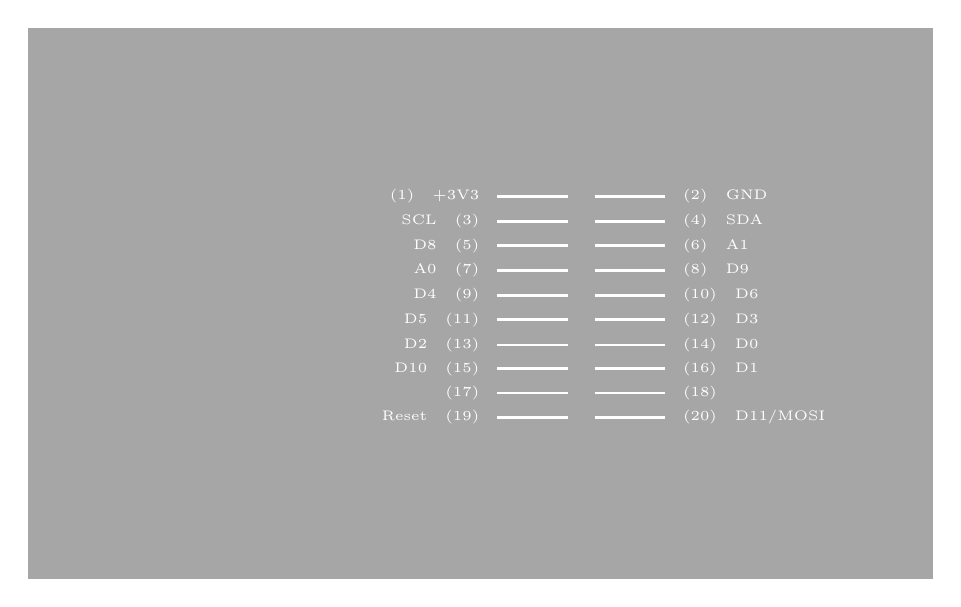
\begin{tikzpicture}
        \ArduinoNanoShieldTikz
        
        \fill[gray, opacity=0.7] (0,30) rectangle (11.5,23);
        
        
        \coordinate (A) at (6.61,28.14);
        \coordinate (B) at (7.45,24.81);    
        \begin{scope}
            \clip (A) rectangle (B);
            
            \ArduinoNanoShieldTikz
            
        \end{scope}
        
        
        %   \fill[black] (6.76, 27.97) rectangle (6.95, 27.76);
        \node[left] (Pin1) at (5.86,27.86) {\textcolor{white}{\tiny (1) \; +3V3}};
        \draw[line width=1pt,white] (6.86,27.86) -- (5.96,27.86);
        
        %   \fill[black] (7.09, 27.96) rectangle (7.29, 27.76);
        \node[right] (Pin1) at (8.2,27.86) {\textcolor{white}{\tiny (2) \; GND}};
        \draw[line width=1pt,white] (7.2,27.86) -- (8.1,27.86);
        
        %   \fill[black] (6.76, 27.64) rectangle (6.95, 27.44);
        \node[left] (Pin1) at (5.86,27.54) {\textcolor{white}{\tiny SCL \; (3)}};
        \draw[line width=1pt,white] (6.86,27.54) -- (5.96,27.54);
        
        %   \fill[black] (7.1, 27.63) rectangle (7.29, 27.44);
        \node[right] (Pin1) at (8.2,27.54) {\textcolor{white}{\tiny (4) \; SDA}};
        \draw[line width=1pt,white] (7.2,27.54) -- (8.1,27.54);
        
        %   \fill[black] (6.77, 27.33) rectangle (6.96, 27.13);
        \node[left] (Pin1) at (5.86,27.23) {\textcolor{white}{\tiny D8 \;  (5)}};
        \draw[line width=1pt,white] (6.86,27.23) -- (5.96,27.23);
        
        %   \fill[black] (7.1, 27.32) rectangle (7.29, 27.13);
        \node[right] (Pin1) at (8.2,27.23) {\textcolor{white}{\tiny (6) \; A1}};
        \draw[line width=1pt,white] (7.2,27.23) -- (8.1,27.23);
        
        %   \fill[black] (6.76, 27.02) rectangle (6.96, 26.82);
        \node[left] (Pin1) at (5.86,26.92) {\textcolor{white}{\tiny A0 \;  (7)}};
        \draw[line width=1pt,white] (6.86,26.92) -- (5.96,26.92);
        
        %   \fill[black] (7.1, 27.01) rectangle (7.29, 26.82);
        \node[right] (Pin1) at (8.2,26.92) {\textcolor{white}{\tiny (8)  \; D9}};
        \draw[line width=1pt,white] (7.2,26.92) -- (8.1,26.92);
        
        %   \fill[black] (6.77, 26.7) rectangle (6.96, 26.5);
        \node[left] (Pin1) at (5.86,26.6) {\textcolor{white}{\tiny D4 \; (9)}};
        \draw[line width=1pt,white] (6.86,26.6) -- (5.96,26.6);
        
        %   \fill[black] (7.1, 26.7) rectangle (7.29, 26.5);
        \node[right] (Pin1) at (8.2,26.6) {\textcolor{white}{\tiny (10) \; D6}};
        \draw[line width=1pt,white] (7.2,26.6) -- (8.1,26.6);
        
        %   \fill[black] (6.77, 26.39) rectangle (6.96, 26.19);
        \node[left] (Pin1) at (5.86,26.29) {\textcolor{white}{\tiny D5 \;  (11)}};
        \draw[line width=1pt,white] (6.86,26.29) -- (5.96,26.29);
        
        %   \fill[black] (7.11, 26.38) rectangle (7.3, 26.19);
        \node[right] (Pin1) at (8.2,26.29) {\textcolor{white}{\tiny (12) \; D3}};
        \draw[line width=1pt,white] (7.2,26.29) -- (8.1,26.29);
        
        %   \fill[black] (6.76, 26.08) rectangle (6.96, 25.87);
        \node[left] (Pin1) at (5.86,25.97) {\textcolor{white}{\tiny D2 \; (13)}};
        \draw[line width=1pt,white] (6.86,25.97) -- (5.96,25.97);
        
        %   \fill[black] (7.1, 26.07) rectangle (7.29, 25.87);
        \node[right] (Pin1) at (8.2,25.97) {\textcolor{white}{\tiny (14) \; D0}};
        \draw[line width=1pt,white] (7.2,25.97) -- (8.1,25.97);
        
        %   \fill[black] (6.76, 25.77) rectangle (6.95, 25.57);
        \node[left] (Pin1) at (5.86,25.67) {\textcolor{white}{\tiny D10 \;  (15)}};
        \draw[line width=1pt,white] (6.86,25.67) -- (5.96,25.67);
        
        %   \fill[black] (7.1, 25.76) rectangle (7.29, 25.57);
        \node[right] (Pin1) at (8.2,25.67) {\textcolor{white}{\tiny (16) \; D1}};
        \draw[line width=1pt,white] (7.2,25.67) -- (8.1,25.67);
        
        %   \fill[black] (6.76, 25.46) rectangle (6.95, 25.26);
        \node[left] (Pin1) at (5.86,25.36) {\textcolor{white}{\tiny (17)}};
        \draw[line width=1pt,white] (6.86,25.36) -- (5.96,25.36);
        
        %   \fill[black] (7.1, 25.45) rectangle (7.29, 25.26);
        \node[right] (Pin1) at (8.2,25.36) {\textcolor{white}{\tiny (18)}};
        \draw[line width=1pt,white] (7.2,25.36) -- (8.1,25.36);
        
        %   \fill[black] (6.76, 25.15) rectangle (6.96, 24.94);
        \node[left] (Pin1) at (5.86,25.05) {\textcolor{white}{\tiny Reset \; (19)}};
        \draw[line width=1pt,white] (6.86,25.05) -- (5.96,25.05);
        
        %   \fill[black] (7.1, 25.14) rectangle (7.29, 24.94);
        \node[right] (Pin1) at (8.2,25.05) {\textcolor{white}{\tiny (20) \; D11/MOSI}};
        \draw[line width=1pt,white] (7.2,25.05) -- (8.1,25.05);
        
        
    \end{tikzpicture}    
    
    %    \includegraphics[width=0.9\textwidth]{Nano33BLESense/TinyMLKit/TinyMachineLearningShieldRotated.png}
    \captionof{figure}[Pin-Belegung des Tiny Machine Learning Shields]{Pin-Belegung des Tiny Machine Learning Shields \cite{ArduinoShield:2021}}\label{TinyMachineLearningShieldPins}
\end{center}





\section{Die OV7675 Kamera}

Da die auf dem Arduino fest verbauten Lichtsensoren nur Helligkeit und Farben messen können, ist in dem Kit eine Kamera enthalten. Diese kann verwendet werden, um Objekte zu erkennen oder einen Videostream auszugeben. In unserem Projekt findet die Kamera allerdings keine Verwendung.\newline
Die Kamera kann direkt auf den mittleren Anschluss des Tiny Machine Learning Shields gesteckt werden. Es sind also keine zusätzlichen Kabel zum Verbinden notwendig. 

\begin{figure}[H]
    \centering
    \includegraphics[width=0.8\textwidth]{Nano33BLESense/TinyMLKit/OV7675.jpg}
    \caption[Das OV7675 Kameramodul]{Das OV7675 Kameramodul \cite{ArduinoKit:2022}}
\end{figure}


\section{USB-Micro-B- auf USB-A-Kabel}

Zur Spannungsversorgung ist in der Box ein USB-Micro-B- auf USB-A-Kabel enthalten. Mit diesem können außerdem die Programme auf den Arduino aufgespielt sowie Daten vom Arduino auf das Programmiergerät übertragen werden.

\begin{figure}[H]
    \centering
    \includegraphics[width=0.8\textwidth]{Nano33BLESense/TinyMLKit/USBCable}
    \caption{Ein USB-A auf Micro-USB Kabel}
\end{figure}
\Mynote{Quelle fehlt}




%%%%%%%%%%%%
%
% $Autor: Wings $
% $Datum: 2019-03-05 08:03:15Z $
% $Pfad: LEDPower $
% $Version: 4250 $
% !TeX spellcheck = en_GB/de_DE
% !TeX encoding = utf8
% !TeX root = filename 
% !TeX TXS-program:bibliography = txs:///biber
%
%%%%%%%%%%%%


%todo citations
%todo create tikz pictures
%todo test the code

\chapter{Power LED}\index{LED!Power LED}

Arduino boards have a power LED on board. Normally, the power LED indicates the status of the board.

\section{General Information}

The power LED on an Arduino board is a small, usually red or green, \ac{led} that indicates whether the board is receiving power. It is typically located near the USB connector on the board. When the board is powered on, the \ac{led} will illuminate. The specific color and behavior of the power LED may vary depending on the Arduino board model. For example, on the Arduino Uno, the power LED is red and illuminates steadily when the board is powered on. On the Arduino Nano, the power LED is green and blinks slowly when the board is powered on. The power LED is a helpful visual indicator that can be used to troubleshoot power supply issues. If the power LED is not illuminated, it means that the board is not receiving power. This could be due to a number of reasons, such as a loose USB connection, a damaged power supply, or a problem with the board itself. By checking the power LED, you can quickly identify and resolve power supply problems with your Arduino board. \cite{ArduinoNanoGetStarted:2024,Arduino:2023a,Arduino:2023,ArduinoNano33Manual:2022,Kurniawan:2021b}


\section{Power LED}

While labeled as a power LED, the single green \ac{led} on the Nano 33 BLE Sense isn't solely for power indication. It has multi-functionality depending on board state and user code interaction. During typical operation, it lights steadily green when powered, similar to other Arduino models.
However, it flashes rapidly during serial communication and bootloader mode.
Notably, when user code enters deep sleep mode, the \ac{led} turns off entirely for power saving. This includes power status, communication activity, and sleep mode activation.
Understanding these \ac{led} behaviors can aid in troubleshooting and code debugging.
The green power LED's primary function remains indicating power and basic board states. \cite{ArduinoNanoGetStarted:2024,Arduino:2023a,Arduino:2023,ArduinoNano33Manual:2022}

\begin{center}    
  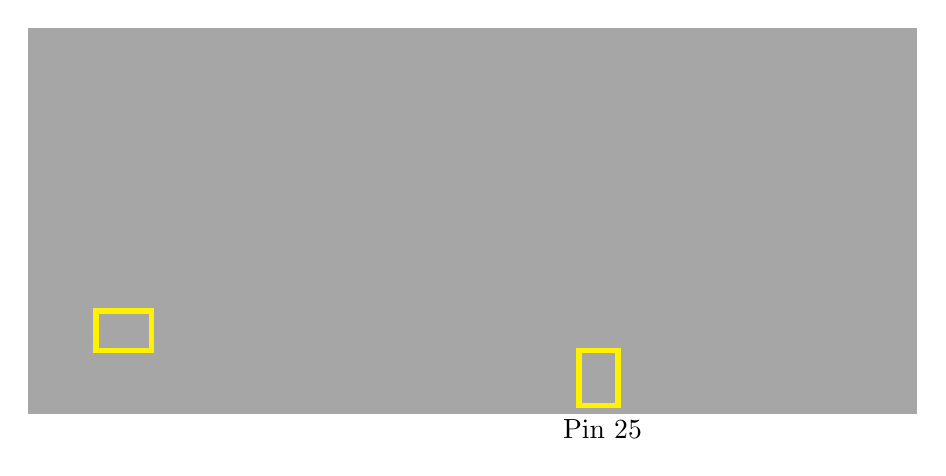
\begin{tikzpicture}
    %\node at (0,0) (Board) {\includegraphics{Arduino/Nano33BLE/Nano33BLESense}};
    
    \ArduinoNanoTikz;

    \fill[gray, opacity=0.7] (-11.2,-0.2) rectangle (0.1,4.7);
    
    \coordinate (A) at (-10.33,0.6);
    \coordinate (B) at (-9.63,1.1);    

    \coordinate (C) at (-4.2,0.6);
    \coordinate (D) at (-3.7,-0.1);    
    
    
    \begin{scope}
      \clip (A) rectangle (B);
      
      \ArduinoNanoTikz

      %\node at (0,0) (Board) {\includegraphics{Arduino/Nano33BLE/Nano33BLESense}};

    \end{scope}


    \draw[yellow,line width=2pt] (A)  rectangle (B);
    \draw[yellow,line width=2pt] (C)  rectangle (D);
    
    \node (P25) at (-3.9, -0.4) {Pin 25};
  \end{tikzpicture}    

  \captionof{figure}{Arduino Nano 33 BLE Sense's Power LED with Pin 25}  
\end{center}


    

\section{Specification}


\subsection{Pin Assignment}

The power LED is a green \ac{led} and connected to pin 25.\index{Pin!Pin 25} The brightness can be controlled via \ac{pwm}. \cite{Arduino:2023a,Arduino:2023}

\begin{description}
    \item [Power LED:] \PYTHON{LED\_PWR =  25u}
\end{description}

Power LED is active-high and connected to pin 25.

The power LED can also be controlled programmatically by setting the pin to \PYTHON{HIGH} or \PYTHON{LOW}. 


The pin must be defined as an output in the function \PYTHON{setup} by setting \PYTHON{pinMode (LED\_PWR, OUTPUT)}, otherwise the \ac{led} cannot be switched on.

\medskip 


%Let's say we have a 200 Ohm resistor. With 5V from the Arduino and 2V across the LED, that leaves 3V across the resistor. Using [u]Ohm's Law[/u] 4, we can calculate the current. 3V/200 Ohms = 0.015 Amps (15mA). The same 15mA is flowing through the LED with 2V across it, so we have 30mW of power dissipated in the LED (2V x 15mA). Plus 45mW wasted in the resistor (3V x 15mA). Or if you want the total power coming out of the Arduino, 5V x 15mW = 75mW, which is the same as 30mW + 45mW.

\subsection{Power Comsumption}\label{LEDPowerComsumption}

The power comsumption has to be considered. There, the power and current in a simple circuit using a resistor and an LED has to calculated.

The led onboard works in a circuit with an 200 Ohm resistor, a 5V power source from an Arduino, and an LED with 2V across it. To find out how much power is being used by the LED and the resistor, the current must be calculated in the first step. Using Ohm's Law $V = I \cdot R$ we can find the current flowing through the resistor. Since 3V is across the resistor, we can plug in the values:

\medskip

$$\frac{3\hbox{V}}{200 \Omega} = 0.015 \hbox{A} = 15\hbox{mA}$$

\medskip

This means that $15$mA of current is flowing through the resistor and the LED. In the next step, we calculate the power. Now that we know the current, we can calculate the power dissipated in the LED and the resistor.

\begin{itemize}
  \item For the LED: $2$V $\times$ $15$mA $= 30$mW
  \item For the resistor: $3$V $\times$ $15$mA = $45$mW
  \item Total Power:

     To find the total power coming out of the Arduino, we multiply the voltage by the current:

              $5$V $\times$ $15$mA = $75$mW
\end{itemize}

\medskip

Notice that the total power (75mW) is equal to the sum of the power dissipated in the LED (30mW) and the resistor (45mW). This makes sense, since all the power coming out of the Arduino is being used by either the LED or the resistor.


\medskip

The pin 25 can also be used otherwise. Then the \ac{led} is just switched on if the board is connected to a power source. %\Mynote{to be tested!}

%\Mynote{What happen if there is another \ac{led} at the pin? Both in use?}

%\section{Calibration}
%
%cite method

\section{Simple Code}

\subsection{Simple Code for LEDs}

Using of LEDs is a standard problem for Arduino's programmer. Therefore, a simple library is introduced here.

\medskip

In the header file \FILE{LED.h}, see code \ref{Nano:LEDHeader}, are the declaration of the functions. There are 3 functions:

\begin{enumerate}
    \item \PYTHON{LEDinit}: This funtion initializes a digital pin of the LED as an output.
    \item \PYTHON{LED}: This funtion switches the LED  on or off.
    \item \PYTHON{LEDBrightness}: This funtion sets the LED's brightness.
\end{enumerate}

{
    \captionof{code}{Header file without comments  for using a LED}\label{Nano:LEDHeader}
    \ArduinoExternal{linerange={12-17,33-34,47-48,63-64,67}}{../../Code/Nano33BLESense/LEDs/LED.h}
}

In the file \FILE{LED.cpp}, see code \ref{Nano:LEDCpp}, the functions are implemented.

{
    \captionof{code}{Code file without comments for using a LED}\label{Nano:LEDCpp}
    \ArduinoExternal{linerange={9-11,26-32,45-57,71-89}}{../../Code/Nano33BLESense/LEDs/LED.cpp}
}


\subsection{Simple Code for the Power LED}

For using the power  LED, a simple library is introduced here.

\medskip


In the header file \FILE{PowerLED.h}, see code \ref{Nano:PowerLEDHeader}, are the declaration of the variables and the  functions. A variable is connected to pin 25.\index{Pin!Pin 25} The pin 25 is defined as an output in the function \PYTHON{PowerLEDinit}. There are  2 functions:

\begin{enumerate}
    \item \PYTHON{PowerLEDinit}: This funtion initializes a the digital pin 25 of the power LED as an output.
    \item \PYTHON{PowerLED}: This funtion switches the power LED  on or off.
\end{enumerate}

{
    \captionof{code}{Header file with doxygen comments for using the Power LED}\label{Nano:PowerLEDHeader}
    \ArduinoExternal{linerange={9-14,27-28,40-42}}{../../Code/Nano33BLESense/LEDs/PowerLED.h}
}

In the file \FILE{PowerLED.cpp}, see code \ref{Nano:PowerLEDCpp}, the functions are implemented.

{
    \captionof{code}{Code file with doxygen comments for using the Power LED}\label{Nano:PowerLEDCpp}
    \ArduinoExternal{linerange={12-15,28-34,46-51}}{../../Code/Nano33BLESense/LEDs/PowerLED.cpp}
}


\subsection{Simple Code for Testing the Power LED}


In the sketch \ref{Nano:PowerLEDTest}, the power LED is tested. First, the function \PYTHON{PowerLEDinit} is called in the  function \PYTHON{setup}. In the function \PYTHON{loop}, the power LED is switched on for 1 second and switched off for 1 second so that the power LED flashes accordingly.



{
  \captionof{code}{Simple sketch to control the power LED}\label{Nano:PowerLEDTest}
  \ArduinoExternal{linerange={16-18,30-34,46-56}}{../../Code/Nano33BLESense/Test/TestLEDPower.ino}
}

\bigskip

This is just a simple example. The variable \PYTHON{LED\_PWR} is already defined, so the assignment is not necessary. The command \PYTHON{delay} should be avoided in an Arduino sketch. Instead, variables of the type \PYTHON{elapsedMillis} should be used. \cite{ArduinoLanguage:2024}

%\Mynote{Arduino Referenz \url{https://github.com/pfeerick/elapsedMillis/wiki}}




\subsection{Test all Functions}

The brightness of the power LED can be controlled. This is demonstrated in the example sketch \ref{Nano:PowerLEDTestPWM}.

Using the pulse width modulation, the brightness is gradually increased to the maximum value and then gradually reduced to 0 again.




{
    \captionof{code}{Simple sketch to check the battery state using the power LED}\label{Nano:PowerLEDTestPWM}
    \ArduinoExternal{linerange={11-18,30-34,46-60}}{../../Code/Nano33BLESense/Test/TestLEDPowerBrightness.ino}
}



\section{Simple Application}

There are different situations where it might be useful to program the power LED of the Arduino Nano. For example, you could use it to:

\begin{itemize}
    \item Indicate the status of the board, such as whether it is connected to a power source, a computer, or a sensor.
    \item  Display the battery level of the board, by changing the brightness or color of the power \ac{led}.
    \item Create a visual alarm or notification, by making the power LED blink or flash in a certain pattern.
\end{itemize}

\medskip

The next sketch is a frame for applications with a sign of life. The power LED is switched on for 1 sec and off for 29 sec. The file \FILE{SignsOfLife.h}, see \ref{Nano:SignsOfLife}, contains the declarations and the file \FILE{SignsOfLife.cpp} contains the implementations. 


{
    \captionof{code}{Simple code for signs of life}\label{Nano:SignsOfLife}
    \ArduinoExternal{linerange={11-25,43-44,56-61}}{../../Code/Nano33BLESense/LEDs/SignsOfLife.h}\label{Nano:SignsOfLifeHeader}
}


The library contains one function for initialization and one function \PYTHON{SignsOfLife}, which controls the LED.


{
    \captionof{code}{Simple code for signs of life}\label{Nano:SignsOfLife}
    \ArduinoExternal{linerange={11-13,31-52,64-84}}{../../Code/Nano33BLESense/LEDs/SignsOfLife.cpp}\label{Nano:SignsOfLifecpp}
}


\medskip


A simple application is to check the condition of the battery. The sktech \ref{Nano:PowerLEDTestBattery} demonstrates, if the voltage drops too low, the power LED flashes, see \cite{Scherer:2022} for more information.

{
    \captionof{code}{Simple sketch to check the battery state using the power LED}\label{Nano:PowerLEDTestBattery}
    \ArduinoExternal{linerange={11-18,31-35,48-88,98-105}}{../../Code/Nano33BLESense/Test/TestLEDPowerBattery.ino}
}


\section{Further Readings}

\begin{itemize}
  \item Kurniawan, Agus: \textsl{IoT Projects with Arduino Nano BLE Sense: Step-By-Step Projects for Beginners}. Apress, 2021. \cite{Kurniawan:2021b}
  \item K\"uhnel, Claus: \textsl{Arduino - Das umfassende Handbuch}. Rheinwerk Verlag GmbH, 2024. \cite{Kuehnel:2024}
  \item Smythe, Richard J.: \textsl{Advanced Arduino Techniques in Science - Refine Your Skills and Projects with PCs or Python-Tkinter}. Apress, 2021. \cite{Smythe:2021}
  \item Smythe, Richard J.: \textsl{Arduino in Science - Collecting, Displaying, and Manipulation Sensor Data}. Apress, 2021. \cite{Smythe:2021b}
\end{itemize}      




%%%%%%%%%%%%
%
% $Autor: Wings $
% $Datum: 2019-03-05 08:03:15Z $
% $Pfad: LEDBuiltIn $
% $Version: 4250 $
% !TeX spellcheck = en_GB/de_DE
% !TeX encoding = utf8
% !TeX root = filename 
% !TeX TXS-program:bibliography = txs:///biber
%
%%%%%%%%%%%%

%todo citations
%todo create tikz pictures
%todo test the code


\chapter{Built-inLED}\index{LED!Built-in LED}

Some Arduino boards have a LED on board which can use for the application. \cite{ArduinoNanoGetStarted:2024,Arduino:2023a,Arduino:2023}

\section{General Information}

LEDs are used in the applications. Depending on the action performed by a user or the sketch, corresponding feedback can be provided. This can take the form of the LED switching on, switching off or flashing. \cite{Kurniawan:2021b}




\section{Built-in LED}

The built-in LED of the Arduino Nano 33 BLE Sense is a single orange LED that is connected to pin 13 on the board. The built-in LED is active-high, which means that setting the pin to \PYTHON{HIGH} will turn the LED on, and setting the pin to \PYTHON{LOW} will turn the LED off. The built-in LED can be used for various purposes, such as indicating the status of the board, displaying sensor data, creating visual effects, or debugging. \cite{Arduino:2023a,Arduino:2023,ArduinoNano33Manual:2022}


\bigskip



\begin{center}    
    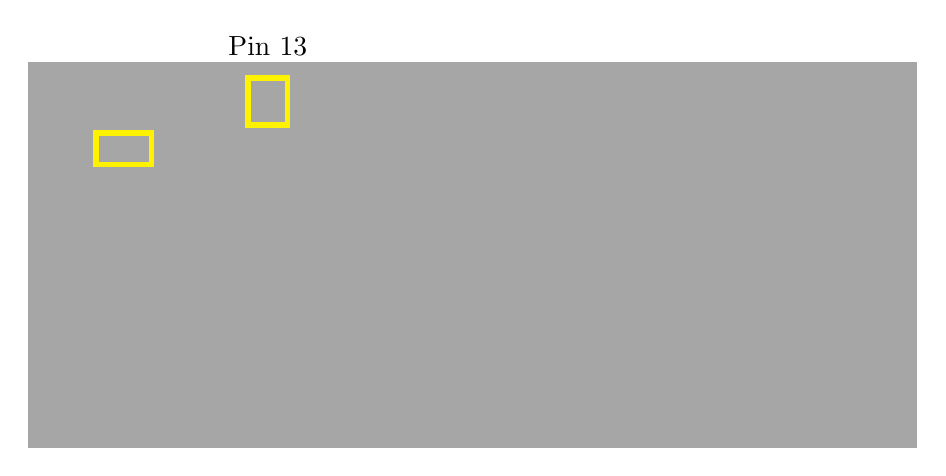
\begin{tikzpicture}
        %\node at (0,0) (Board) {\includegraphics{Arduino/Nano33BLE/Nano33BLESense}};
        
        \ArduinoNanoTikz;
        
        \fill[gray, opacity=0.7] (-11.2,-0.2) rectangle (0.1,4.7);
        
        \coordinate (A) at (-10.33,3.4);
        \coordinate (B) at (-9.63,3.8); 
           
        
        \coordinate (C) at (-8.4,3.9);
        \coordinate (D) at (-7.9,4.5);  
        
        \def\cliparea{(C) rectangle (D); (A) rectangle (B); }  
        
        \begin{scope}
          \clip (A) rectangle (B);
            
            \ArduinoNanoTikz
            
            %\node at (0,0) (Board) {\includegraphics{Arduino/Nano33BLE/Nano33BLESense}};
            
        \end{scope}
    
%        \fill[ArduinoColor] (C) rectangle (D);
%         \fill[gray!30] ({-8.16-0.195},4.145) rectangle ++(0.39, 0.39); 
%        \draw[fill=gray!30,gray!30] (-8.145,4.143) circle(0.195); 
%        \draw[fill=gray!60,gray!60] (-8.145,4.143) circle(0.165); 
%        \fill[white,white](-8.145,{4.143+0.39}) circle (0.1275);
        
        \draw[yellow,line width=2pt] (A)  rectangle (B);
        \draw[yellow,line width=2pt] (C)  rectangle (D);
        
        \node (P25) at (-8.15, 4.9) {Pin 13};
    \end{tikzpicture}    
  
 

  \captionof{figure}{Arduino Nano 33 BLE Sense's built-in LED  with Pin 13}  
\end{center}
    

\section{Specification}

\subsection{Pin Assignment}

The built-in LED is a orange LED and connected to pin 13.\index{Pin!Pin 13} The brightness can not be controlled. \cite{Arduino:2023a,Arduino:2023}

\begin{description}
    \item [Built-in LED:] \PYTHON{LED\_BUILTIN =  13u}
\end{description}

Built-in LED is active-high and connected to pin 13.

The built-in LED can be controlled programmatically by setting the pin to \PYTHON{HIGH} or \PYTHON{LOW}. 


%\Mynote{cite data sheet, power consumption?}

The pin 13 must be defined as an output in the function \PYTHON{setup} by setting \PYTHON{pinMode (13, OUTPUT)}, otherwise the LED cannot be switched on.

\medskip 


The pin 13 can also be used otherwise. Then the LED is not in use.

%\Mynote{What happen if there is another LED at the pin? Both in use?}


\subsection{Power Comsumption}

The power comsumption has to be considered. It is the same value as for the power LED, see section~\ref{LEDPowerComsumption}.


%\section{Calibration}
%
%cite method

\section{Simple Code}

\subsection{Simple Code for the Built-in LED}

For using the built-in LED, a simple library is introduced here.

\medskip


In the header file \FILE{BuiltinLED.h}, see code \ref{Nano:BuiltinLEDHeader}, are the declaration of the variables and the  functions. A variable is connected to pin 13.\index{Pin!Pin 13} The pin 13 is defined as an output in the function \PYTHON{BuiltinLEDinit}. There are  2 functions:

\begin{enumerate}
    \item \PYTHON{BuiltinLEDinit}: This funtion initializes the digital pin 13 of the built-in LED as an output.
    \item \PYTHON{BuiltinLED}: This funtion switches the built-in LED  on or off.
\end{enumerate}

{
    \captionof{code}{Header file without comments for using the Built-in LED}\label{Nano:BultinLEDHeader}
    \ArduinoExternal{linerange={9-14,27-28,40-42}}{../../Code/Nano33BLESense/LEDs/BuiltinLED.h}
}

In the file \FILE{BuiltinLED.cpp}, see code \ref{Nano:BuiltinLEDCpp}, the functions are implemented.

{
  \captionof{code}{Code file without comments for using the Built-in LED}\label{Nano:BuiltinLEDCpp}
  \ArduinoExternal{linerange={12-15,28-34,46-51}}{../../Code/Nano33BLESense/LEDs/builtinLED.cpp}
}


\subsection{Simple Code for Testing the Built-in LED}

In the sketch \ref{Nano:BuiltinLEDTest}, a variable is connected to pin 13.\index{Pin!Pin 13} The pin is defined as an output in the function \PYTHON{setup}. In the function \PYTHON{loop}, the LED is switched on for 1 second and switched off for 1 second so that the LED flashes accordingly.



{
  \captionof{code}{Simple sketch without comments to control the built-in LED}\label{Nano:BuiltinLEDTest}
  \ArduinoExternal{linerange={17-19,31-34,47-57}}{../../Code/Nano33BLESense/Test/TestLEDBuiltin.ino}
}

\bigskip

This is just a simple example. The variable \PYTHON{LED\_BUILTIN} is already defined, so the assignment is not necessary. The command \PYTHON{delay} should be avoided in an Arduino sketch. Instead, variables of the type \PYTHON{elapsedMillis} should be used.

%\Mynote{Arduino Referenz \url{https://github.com/pfeerick/elapsedMillis/wiki}}

\section{Tests}

\subsection{Simple Function Test}

The simplest test is the flashing of the LED at 2 Hz, see sketch \ref{Nano:BuiltinLEDTest2}.

{
  \captionof{code}{Simple sketch to test the built-in LED}\label{Nano:BuiltinLEDTest2}
  \ArduinoExternal{linerange={17-19,31-34,47-57}}{../../Code/Nano33BLESense/Test/TestLEDBuiltin.ino}
}


\subsection{Test all Functions}

As the built-in does not allow any special manipulations, all functions are covered with the sketch \ref{Nano:BuiltinLEDTest2}.

\section{Simple Application}

In many applications, it is necessary to save power so that the LED is not switched on continuously. Nevertheless, feedback is required as to whether the system, e.g. a fire detector, is switched on and functional. In this case, the LED is switched on for 1 second at a defined time interval, in this case 30 seconds. This is implemented in the example \ref{Nano:TestBuiltinApp}.

{
    \captionof{code}{A simple watch dog: A simple watchdog: the built-in LED is switched on for 1 second every 30 seconds.}\label{Nano:TestBuiltinApp}
    \ArduinoExternal{linerange={13-22,35-43,56-62}}{../../Code/Nano33BLESense/Test/TestLEDBuiltinApplication.ino}
}



\section{Further Readings}

\begin{itemize}
    \item Babu, Neelakandan Ramesh and  Chenchireddy, Kalagotla and  Reddy, V. Harsha Vardhan and  Samhitha, Dr. and Apparao, P. and  Kalyan, Ch. Pavan: \textsl{Case Study on Ni-MH Battery}. 2023 2\textsuperscript{nd} International Conference on Applied Artificial Intelligence and Computing (ICAAIC), 2023. \cite{Babu:2023}
    \item Scherer, Thomas: \textsl{Elektor special: Stromversorgung und Batterien}. Elektor Special. 2022. \cite{Scherer:2022}
\end{itemize}





%%%
%
% $Autor: Wings $
% $Datum: 2021-05-14 $
% $Pfad: ArduinoLEDRGB $
% $Dateiname: 
% $Version: 4620 $
%
% !TeX spellcheck = de_DE/GB
% !TeX program = pdflatex
% !BIB program = biber/bibtex
% !TeX encoding = utf8
%
%%%

%todo citations
%todo create tikz pictures
%todo create sketches /ino-files with the code
%todo test the code


%https://projecthub.arduino.cc/semsemharaz/interfacing-rgb-led-with-arduino-b59902

% Farben: https://rgbcolorcode.com/color/00FF00


\chapter{Built-in RGB-LED}\index{LED!Built-in RGB-LED}

Some Arduino boards have a RGB-LED on board which can use for the application. ARG-LED is at least thre LEDs in on.

\section{General Information}

An RGB LED is a type of \ac{led} that can emit different colors of light. RGB stands for red, green, and blue, which are the three primary colors of light. An RGB LED consists of three individual \ac{led}s inside a single package, each with its own color and pin. By varying the brightness of each \ac{led} using \ac{pwm} signals, an RGB LED can produce a wide range of colors by mixing the primary colors. An RGB LED is usually active-low, which means that setting the pin to LOW will turn the \ac{led} on, and setting the pin to HIGH will turn the \ac{led} off. \cite{Bernstein:2018,Hering:2021,Karvinen:2014}

%\Mynote{cite English books}

\section{Specific Sensor}

The onboard LED of the Arduino Nano 33 BLE Sense is a RGB-LED that consists of three individual \ac{led}s: red, green, and blue. Each \ac{led} is connected to a different pin on the board:

\begin{itemize}
    \item Pin 22 for red,
    \item Pin 23 for green, and 
    \item Pin 24 for blue.
\end{itemize} 



The RGB-LED can produce different colors by varying the brightness of each \ac{led} using \ac{pwm} signals. The RGB-LED is active-low, which means that setting the pin to \PYTHON{LOW} will turn the \ac{led} on, and setting the pin to \PYTHON{HIGH} will turn the \ac{led} off. This is different from the power LED and the built-in LED, which are both active-high. \cite{ArduinoNanoGetStarted:2024,Arduino:2023a,Arduino:2023}



\bigskip

\begin{center}    
    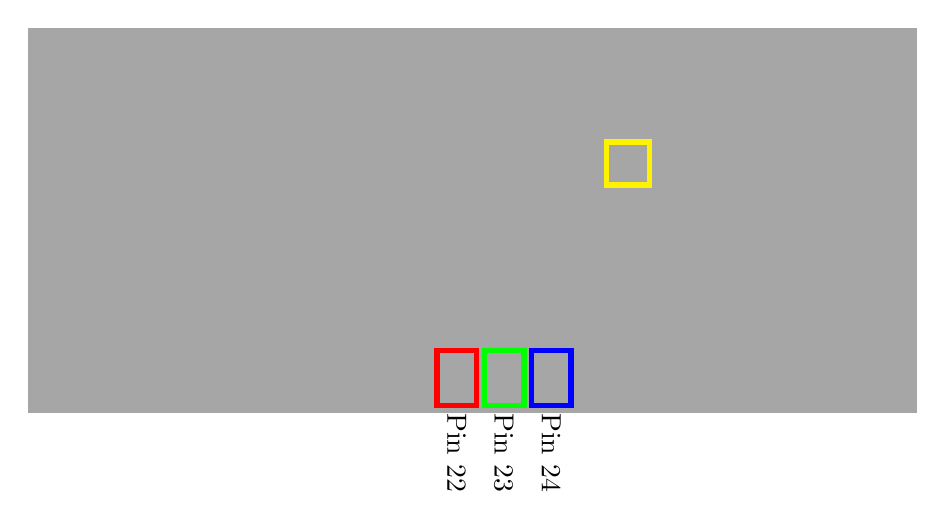
\begin{tikzpicture}
        %\node at (0,0) (Board) {\includegraphics{Arduino/Nano33BLE/Nano33BLESense}};
        
        \ArduinoNanoTikz;
        
        \fill[gray, opacity=0.7] (-11.2,-0.2) rectangle (0.1,4.7);
        
        \coordinate (A) at (-3.85,3.25);
        \coordinate (B) at (-3.3,2.7);    
        
        \coordinate (C) at (-4.8,0.6);
        \coordinate (D) at (-4.3,-0.1);    

        \coordinate (E) at (-5.4,0.6);
        \coordinate (F) at (-4.9,-0.1);    

        \coordinate (G) at (-6.0,0.6);
        \coordinate (H) at (-5.5,-0.1);    
        
        
        \begin{scope}
            \clip (A) rectangle (B);
            
            \ArduinoNanoTikz
            
            %\node at (0,0) (Board) {\includegraphics{Arduino/Nano33BLE/Nano33BLESense}};
            
        \end{scope}
        
        
        \draw[yellow,line width=2pt] (A)  rectangle (B);
        \draw[blue,line width=2pt] (C)  rectangle (D);
        \draw[green,line width=2pt] (E)  rectangle (F);
        \draw[red,line width=2pt] (G)  rectangle (H);
        
        \node[rotate=-90] (P25) at (-4.55, -0.7) {Pin 24};
        \node[rotate=-90] (P25) at (-5.15, -0.7) {Pin 23};
        \node[rotate=-90] (P25) at (-5.75, -0.7) {Pin 22};
    \end{tikzpicture}    
    
    \captionof{figure}{Arduino Nano 33 BLE Sense's RGB LED with Pin 22, Pin 23, and Pin 24}  
\end{center}

\bigskip



The brightness of the LED varies between 5000-6000 \ac{mcd} at a current of 20 mA. The color temperature is controllable and can be set in a range of 5000-6000 Kelvin. The LED should be stored and used between -40$^\circ$C and +85$^\circ$C.



\section{Specification}

\subsection{Pin Assignment}

The RGB LED occupies pins on the board internally. These pins are defined via variable names \PYTHON{LEDR}, \PYTHON{LEDG}, and \PYTHON{LEDB}. \cite{Arduino:2023a,Arduino:2023}

This must be observed when using the pins.



\begin{description}
    \item [Red LED:] LEDR = Pin 22\index{Pin!Pin 22,23,24}
    \item [Green LED:] LEDG = Pin 23
    \item [Blue LED:] LEDB = Pin 24
\end{description}


RGB LED is active-low and connected to pin 22, 23, and 24.

The RGB LED can be controlled programmatically by setting the pin to \PYTHON{LOW} or \PYTHON{HIGH}. 


%\Mynote{cite data sheet, power consumption?}

The pins 22, 23, and 24 must be defined as an output in the function \PYTHON{setup} by setting \PYTHON{pinMode (22, OUTPUT)}, \PYTHON{pinMode (23, OUTPUT)} and \PYTHON{pinMode (22, OUTPUT)}, otherwise the \ac{led} cannot be switched on.

\medskip 


The pins 22, 23, 24 can also be used otherwise. Then the \ac{led} is not in use.

\subsection{Power Comsumption}

The power comsumption has to be considered. It is the same value as for the power LED, see section~\ref{LEDPowerComsumption}. Here, a RGB-LED has 3 LEDs inside, therefore the poswer consumption must be consiederd for each color.




\section{Simple Code}


In the header file \FILE{RGBLED.h}, see code \ref{Nano:RGBLEDHeader}, are the declaration of the variables and the  functions. Variables are connected to pin 22, pin 23, and pin 24.\index{Pin!Pin 22}\index{Pin!Pin 23}\index{Pin!Pin 24} The pins are defined as output in the function \PYTHON{RGBLEDinit}. There are the following functions:

\begin{enumerate}
    \item \PYTHON{RGBLEDinit}: This funtion initializes the digital pin 22, pin 23, and pin 24 of the RGB-LED as output.
    \item \PYTHON{RGBLED\_Red}: This funtion switches the red part of the RGB-LED  on or off.
    \item \PYTHON{RGBLED\_Green}: This funtion switches the green part of the RGB-LED  on or off.
    \item \PYTHON{RGBLED\_Blue}: This funtion switches the blue part of the RGB-LED  on or off.
    \item \PYTHON{RGBLED\_Color}: This functions combines the colors.
\end{enumerate}

{
    \captionof{code}{Header file without comments for using the RGB-LED}\label{Nano:RGBLEDHeader}
    \ArduinoExternal{linerange={9-14,27-28,40-42}}{../../Code/Nano33BLESense/LEDs/RGBLED.h}
}

In the file \FILE{RGBLED.cpp}, see code \ref{Nano:RGBLEDCpp}, the functions are implemented.

{
    \captionof{code}{Code file without comments for using the RGB-LED}\label{Nano:RGBLEDCpp}
    \ArduinoExternal{linerange={12-15,28-34,46-51}}{../../Code/Nano33BLESense/LEDs/RGBLED.cpp}
}


\section{Tests}

\subsection{Simple Function Test}

The simplest test is the flashing of the \ac{led}s at 2 Hz, see sketch \ref{Nano:RGBEDTest}.

{
    \captionof{code}{Simple sketch to test the RGB LED}\label{Nano:RGBLEDTest}
    \ArduinoExternal{}{../../Code/Nano33BLESense/Test/TestLEDRGB.ino}
}


\subsection{Test all Functions}

\subsubsection{Different Colors}


\subsubsection{Colors}\index{LED!Colors}

A RGB LED is a device that can emit light of different colors by mixing the primary colors of red, green, and blue. The color of the light depends on the relative brightness of each \ac{led}, which can be controlled by \ac{pwm} signals. By varying the brightness of each \ac{led}, the RGB LED can produce a wide range of colors, such as yellow, cyan, magenta, white, and more. Some examples of the colors and their corresponding brightness values are:

\begin{description}
    \item [Red:] red = 255, green = 0, blue = 0
    \item [Green:] red = 0, green = 255, blue = 0
    \item [Blue:] red = 0, green = 0, blue = 255
    \item [Yellow:] red = 255, green = 255, blue = 0
    \item [Cyan:] red = 0, green = 255, blue = 255
    \item [Magenta:] red = 255, green = 0, blue = 255
    \item [White:] red = 255, green = 255, blue = 255
    \item [Black:] red = 0, green = 0, blue = 0
\end{description}

\medskip

The RGB LED can also create intermediate colors by using different brightness values for each \ac{led}. For example, to create

\begin{itemize}
    \item \textbf{orange}, one can use red = 255, green = 127, blue = 0. 
    \item To create \textbf{pink}, one can use red = 255, green = 192, blue = 203. 
    \item To create \textbf{purple}, one can use red = 128, green = 0, blue = 128. 
\end{itemize}


\bigskip

The sketch \ref{Nano:RGBLEDTestColors} tests different colors of the \ac{led}. The color of the \ac{led} changes every 1 second.

{
  \captionof{code}{value between 0 and 255  to write to the RGB LED}\label{Nano:RGBLEDTestColors}

  \ArduinoExternal{}{../../Code/Nano33BLESense/Test/TestLEDRGBColors.ino}
}



\subsubsection{Brightness of the RGB-LED}\index{LED!Brightness}

The RGB-LED can also create gradients of colors by changing the brightness values gradually over time. This can create a smooth transition from one color to another, such as from red to green to blue and back to red.

This sketch \ref{RGBLEDBrightness} will make the RGB-LED change colors smoothly by varying the brightness of each \ac{led} with different speeds. You can adjust the initial brightness values and the increment/decrement values to get different effects.


{
   \captionof{code}{Different brightness levels for the RGB-LED colors}\label{RGBLEDBrightness}
   \ArduinoExternal{}{../../Code/Nano33BLESense/Test/TestLEDRGBBrightness.ino}
}


\section{Simple Application}

In many applications, it is necessary to save power so that the \ac{led} is not switched on continuously. Nevertheless, feedback is required as to whether the system, e.g. a fire detector, is switched on and functional. In this case, the \ac{led} is switched on for 1 second at a defined time interval, in this case 30 seconds. This is implemented in the example \ref{Nano:TestRGBLEFApp}.

{
    \captionof{code}{A simple watch dog: A simple watchdog: the built-in RGB-LED is switched on for 1 second every 30 seconds.}\label{Nano:TestRGBLEDApp}
    \ArduinoExternal{}{../../Code/Nano33BLESense/Test/TestLEDRGBApplication.ino}
}



\section{Further Readings}

\begin{itemize}
  \item  Schanda, Janos: \textsl{Colorimetry: Understanding the CIE System}. Wiley, 2007. \cite{schanda:2007}
   \item Hiller, Gabrielle: \textsl{Color measurement - the CIE color space}. Datacolor, 2019. \cite{hiller:2019}
   \item Lukac, Rastislav and Plataniotis, Konstantinos N.: \textsl{Color Image Processing: Methods and Applications}. CTC Press, 2018. \cite{lukac:2018}
\end{itemize}



%%%%%%%%%%%%%%%%%%%%%%%%%%%%%%%%%%%%%%%%%%%%%%%%%%%%%%%%%




%%%%%%%%%%%%
%
% $Autor: Wings $
% $Datum: 2019-03-05 08:03:15Z $
% $Pfad: PushButton $
% $Version: 4250 $
% !TeX spellcheck = en_GB/de_DE
% !TeX encoding = utf8
% !TeX root = filename 
% !TeX TXS-program:bibliography = txs:///biber
%
%%%%%%%%%%%%

% Structure
\chapter{Built-in Push Button}\index{Push Button! Built-in Push Button}

\section{General}

A push button is a simple switch mechanism used to control various devices and processes. It is typically made of hard materials like plastic or metal.
The surface of a push button is designed to be easily depressed or pushed by the human finger or hand. When you press a push button, it either closes or opens an electrical circuit. 

In industrial and commercial applications, push buttons can be linked together so that pressing one button releases another. Emergency stop buttons, often with large mushroom-shaped heads, enhance safety in machines and equipment. Pilot lights are sometimes added to push buttons to draw attention and provide feedback when the button is pressed. Color-coding is common to associate push buttons with their specific functions (e.g., red for stopping, green for starting). \cite{DIN:13850}

%\Mynote{cite books, applications, board\\ image of the board}






\section{Built-in Push Button}

The Arduino Nano 33 BLE Sense features an onboard push button. This button is a simple electrical switch that can be activated by pressing it. When you press the button, it completes an electrical circuit. The push button is designed for user interaction and can be used for various purposes.

The built-in button \PYTHON{BUTTON\_B} is connected with pin 11.\index{Pin!Pin 11} Using the function \PYTHON{pinMode(BUTTON\_PIN, INPUT\_PULLUP)} the pin is declared as an input. As can be seen in the sketch, pressing the button can be used to trigger actions; typical actions include switching on an LED, changing modes, or initiating sensor readings.
Overall, the push button provides a convenient way to interact with the Arduino Nano 33 BLE Sense and create responsive projects. \cite{Arduino:2023a,Arduino:2023,ArduinoNano33Manual:2022}


\bigskip



\begin{center}    
    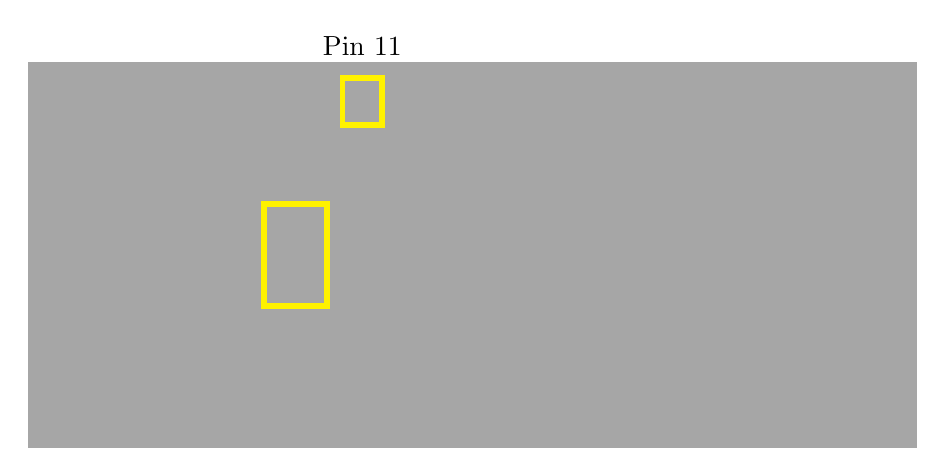
\begin{tikzpicture}
        %\node at (0,0) (Board) {\includegraphics{Arduino/Nano33BLE/Nano33BLESense}};
        
        \ArduinoNanoTikz;
        
        \fill[gray, opacity=0.7] (-11.2,-0.2) rectangle (0.1,4.7);
        
        \coordinate (A) at (-8.2,1.6);
        \coordinate (B) at (-7.4,2.9); 
        
        
        \coordinate (C) at (-7.2,3.9);
        \coordinate (D) at (-6.7,4.5);  
        
        \def\cliparea{(C) rectangle (D); (A) rectangle (B); }  
        
        \begin{scope}
            \clip (A) rectangle (B);
            
            \ArduinoNanoTikz
            
            %\node at (0,0) (Board) {\includegraphics{Arduino/Nano33BLE/Nano33BLESense}};
            
        \end{scope}
        
        %        \fill[ArduinoColor] (C) rectangle (D);
        %         \fill[gray!30] ({-8.16-0.195},4.145) rectangle ++(0.39, 0.39); 
        %        \draw[fill=gray!30,gray!30] (-8.145,4.143) circle(0.195); 
        %        \draw[fill=gray!60,gray!60] (-8.145,4.143) circle(0.165); 
        %        \fill[white,white](-8.145,{4.143+0.39}) circle (0.1275);
        
        \draw[yellow,line width=2pt] (A)  rectangle (B);
        \draw[yellow,line width=2pt] (C)  rectangle (D);
        
        \node (P25) at (-6.95, 4.9) {Pin 11};
    \end{tikzpicture}    
    
    
    
    \captionof{figure}{Arduino Nano 33 BLE Sense's built-in Push Button  with Pin 11}  
\end{center}

\section{Specification}

The built-in button is a small white button  and connected to pin 11.\index{Pin!Pin 11}

\begin{description}
    \item [Built-in Button:] \PYTHON{BUTTON\_B =  11u}
\end{description}

If the pin is declared as input in the function \PYTHON{setup}, then it can be used.

%\Mynote{cite data sheet, power consumption?}

The pin 11 must be defined as an input in the function \PYTHON{setup} by setting \PYTHON{pinMode (11, INPUT\_PULLUP)}, otherwise the button cannot be read.

\medskip 


The pin 11 can also be used otherwise. Then the button is not in use. \cite{Arduino:2023a,Arduino:2023,ArduinoNano33Manual:2022}

%\Mynote{What happen if there is another button at the pin? Both in use?}


\begin{itemize}
  \item cite data sheet
  \item Circuit Diagram
\end{itemize}


\section{Simple Code}


As soon as the button is connected, it can be used. It is not necessary to install a special library. Programming takes place in two steps:

\begin{enumerate}
    \item In the first step, the pin is configured in the function \PYTHON{setup}:
    
    {
        \captionof{code}{Defining the built-in button's pin as an input.}
        \begin{Arduino}
            pinMode(BUTTON_B, INPUT_PULLUP)   
        \end{Arduino}
    }
    \item In the second step, the button can be used in the function \PYTHON{loop}. To read in the value, use the function \PYTHON{digitalRead}:
    
    {
        \captionof{code}{Read the built-in button's state}
        \begin{Arduino}
            buttonState = digitalRead(BUTTON_B);
        \end{Arduino}
    }
    
\end{enumerate}




\section{Tests}


The simplest test is the flashing of an LED for 2 seconds, if the button is pressed, see sketch \ref{Nano:BuiltinButtonTest}.

{
    \captionof{code}{Simple sketch to test the push button and the built-in LED}\label{Nano:BuiltinButtonTest}
    \ArduinoExternal{}{../../Code/Nano33BLESense/Test/TestPushButton.ino}
}




\section{Simple Application}


In the sketch \ref{Nano:TestButtonInterrupt}, pressing the push button triggers an interrupt. The interrupt function is defined, changing the state of a flag. If the flag has the value \PYTHON{true}, the built-in LED is switched on for 2 seconds. After the 2 seconds, the built-in LED is switch off and the value of the flag is set to \PYTHON{false} back. \cite{ArduinoInterrupt:2019}


{
    \captionof{code}[Simple sketch connects the push button with an interrupt.]{Simple sketch connects the push button with an interrupt. Here, pushing the built-in button is handled by an interrupt. Then the built-in LED switch on for 2 sec.}\label{Nano:TestButtonInterrupt}
    \ArduinoExternal{}{../../Code/Nano33BLESense/Test/TestPushButtonInterrupt.ino}
}

\bigskip

This is just a simple example. The variable \PYTHON{BUTTON\_B} is already defined, so the assignment is not necessary. The command \PYTHON{delay} should be avoided in an Arduino sketch. Instead, variables of the type \PYTHON{elapsedMillis} should be used.



\section{Further Readings}

\begin{itemize}
  \item Boxall, John: \textsl{Arduino Workshop - A Hands-On Introduction with 65 Projects}. No Starch Press, 2021. \cite{Boxall:2021}
  \item Vo{\"s}, Andreas: \textsl{Volumio mit Drehgebern erweitern}. Make Magazin, 2024. \cite{Voss:2024}
  \item K\"uhnel, Claus: \textsl{Arduino - Das umfassende Handbuch}. Rheinwerk Verlag GmbH, 2024. \cite{Kuehnel:2024}
\end{itemize}



%%%%%%%%%%%%
%
% $Autor: Wings $
% $Datum: 2019-03-05 08:03:15Z $
% $Pfad: TemplateSensor $
% $Version: 4250 $
% !TeX spellcheck = en_GB/de_DE
% !TeX encoding = utf8
% !TeX root = filename 
% !TeX TXS-program:bibliography = txs:///biber
%
%%%%%%%%%%%%

% Structure
\chapter{Sensor}

\textbf{Introduction} 

The ESP32 is built on a dual-core Xtensa LX6 processor, with clock speeds up to 240 MHz, and features a rich set of peripherals, including multiple GPIOs, ADCs, DACs, and PWM outputs, allowing for a wide range of input and output operations. It supports various development environments, such as Arduino IDE \cite{Bipasha:2018}, MicroPython, and Espressif's own ESP-IDF, making it accessible to both hobbyists and professionals. Additionally, the ESP32 is designed for low-power operation, making it suitable for battery-powered projects. Its combination of high performance, connectivity, and low power consumption has made the ESP32 a popular choice for developing smart devices, home automation systems, and other innovative projects in the IoT space \cite{Aquino:2021} .

%%\Mynote{ books, applications, board}

\section{General}

The ESP32 Nano is a powerful and compact microcontroller developed by Espressif Systems, widely recognized for its robust performance and integrated wireless communication capabilities \cite{M:2021}. It is an ideal choice for developers and hobbyists looking to build a variety of Internet of Things (IoT) projects due to its versatility and extensive feature set.
Here's an general information of some of the most commonly used sensors with the ESP32 Nano\cite{Zulfiqar:2024}:

\begin{itemize}
	\item Temperature and Humidity Sensors
	\item Light Sensors
	\item Motion Sensors
	\item Gas Sensors

\end{itemize}

cite books
\begin{circuitikz}
	
	% ESP32 pins
	\draw (4,5) node[anchor=east] {GND} -- (5,5);
	\draw (4,4.5) node[anchor=east] {5V} -- (5,4.5);
	\draw (4,4) node[anchor=east] {Vext} -- (5,4);
	\draw (4,3.5) node[anchor=east] {RX} -- (5,3.5);
	\draw (4,3) node[anchor=east] {TX} -- (5,3);
	\draw (4,2.5) node[anchor=east] {RST} -- (5,2.5);
	\draw (4,2) node[anchor=east] {GPIO0} -- (5,2);
	\draw (4,1.5) node[anchor=east] {GPIO22} -- (5,1.5);
	\draw (4,1) node[anchor=east] {GPIO19} -- (5,1);
	\draw (4,0.5) node[anchor=east] {GPIO23} -- (5,0.5);
	
	\draw (4,0) node[anchor=east] {GPIO18} -- (5,0);
	\draw (4,-0.5) node[anchor=east] {GPIO5} -- (5,-0.5);
	\draw (4,-1) node[anchor=east] {GPIO15} -- (5,-1);
	\draw (4,-1.5) node[anchor=east] {GPIO2} -- (5,-1.5);
	\draw (4,-2) node[anchor=east] {GPIO4} -- (5,-2);
	\draw (4,-2.5) node[anchor=east] {GPIO17} -- (5,-2.5);
	\draw (4,-3) node[anchor=east] {GPIO16} -- (5,-3);
	
	% Sensors connections
	\draw (1,0.5) node[anchor=east] {TDS sensor module}
	to[short] (4,4.5);
	\draw (1,-1) node[anchor=east] {pH sensor module}
	to[short] (4,4.5);
	\draw (1,-3) node[anchor=east] {Temperature sensor}
	to[short] (4,4.5);
	\draw (1.5,-3) to[short] (1.5,0.5);
	
\end{circuitikz}

\section{Specific Sensor}

\subsection{Temperature and Humidity Sensors [DHT22 Sensors]}

The DHT22 is a low-cost digital temperature and humidity sensor with a single wire digital interface\cite{Garcia:2023}. It uses a capacitive humidity sensor and a thermistor to measure the surrounding air and spits out a digital signal on the data pin (no analog input pins needed).

The sensor is calibrated and doesn’t require extra components so you can get the right to measuring relative humidity and temperature.

It is quite simple to use but requires careful timing to grab data. You can only get new data from it once every 2 seconds.

The DHT22 \cite{Jayetileke:2023} is a low-cost digital temperature and humidity sensor with a single wire digital interface. It uses a capacitive humidity sensor and a thermistor to measure the surrounding air and spits out a digital signal on the data pin (no analog input pins needed).

The sensor is calibrated and doesn’t require extra components so you can get the right to measuring relative humidity and temperature.

It is quite simple to use but requires careful timing to grab data. You can only get new data from it once every 2 seconds.

DHT22 \cite{Faroqi:2020} output calibrated digital signal. It utilizes exclusive digital-signal-collecting-technique and humidity sensing technology, assuring its reliability and stability.Its sensing elements is connected with 8-bit single-chip computer.
Every sensor of this model is temperature compensated and calibrated in accurate calibration chamber and the calibration-coefficient is saved in type of programme in OTP memory, when the sensor is detecting, it will cite coefficient from memory.
Small size and low consumption and long transmission distance(20m) enable DHT22 to be suited in all kinds of harsh application occasions.
Single-row packaged with four pins, making the connection very convenien \cite{Ahmad:2021}.

\begin{itemize}
	\item[\checkmark] The DHT22 is a reliable sensor for determining temperature and humidity.
	\item[\checkmark] Since the sensor can be operated with 3.3V as well as 5V, it is suitable for connection to all common boards like RN-Control, Raspberry Pi and all other microcontrollers.
	\item[\checkmark] Besides the operating voltage, only one port needs to be connected to the sensor. 
	\item[\checkmark] The output is serial as a digital bit sequence. This makes the sensor ideal for monitoring the indoor climate or setting up a weather station.
\end{itemize}



cite board

\subsection{Specification}
\subsection{Temperature and Humidity Sensors [DHT22 Sensors] Specification}

%%\textbf{(1) Power and Pins} 
%%Power's voltage should be 3.3-6V DC \cite{Muhamad:2023}. When power is supplied to sensor, don't send any %%instruction to the sensor within one second to pass unstable status. One capacitor valued 100nF can be added %%between VDD and GND for wave filtering.\\ \\

\textbf{(2) Communication and signal} \\
Single-bus data is used for communication between MCU and DHT22, it costs 5mS for single time communication.
Data is comprised of integral and decimal part, the following is the formula for data.
DHT22 send out higher data bit firstly!
DATA=8 bit integral RH data+8 bit decimal RH data+8 bit integral T data+8 bit decimal T data+8 bit check-sum
If the data transmission is right, check-sum should be the last 8 bit of "8 bit integral RH data+8 bit decimal RH data+8 bit integral T data+8 bit decimal T data".
When MCU send start signal, DHT22 change from low-power-consumption-mode to running-mode. When MCU
finishs sending the start signal, DHT22 will send response signal of 40-bit \cite{Malika:2022} data that reflect the relative humidity

\begin{center} % Center the table
	\begin{tabular}{|l|l|} % Specify alignment and vertical lines
		\hline % Top horizontal line
		\textbf{Model} & \textbf{DHT22} \\
		\hline % Horizontal line
		Power supply & 3.3-6V DC \\
		\hline
		Output signal & digital signal via single-bus \\
		\hline
		Sensing element & Polymer capacitor \\
		\hline
		Operating range & humidity 0-100  \\
		\hline
		Accuracy & humidity +-2 RH(Max +-5 RH);  \\
		\hline
		Resolution or sensitivity & humidity 0.1 RH; \\
		\hline
		Repeatability& humidity +-1 RH \\
		\hline
		Humidity hysteresis & +-0.3 RH \\
		\hline
		Long-term Stability  & +-0.5 RH/year \\
		\hline
		Sensing period & Average: 2s \\
		\hline
		Interchangeability & fully interchangeable \\
		\hline
		Dimensions & small size 14*18*5.5mm \\
		
		\hline % Bottom horizontal line
	\end{tabular}
\end{center}

\begin{itemize}
  \item cite data sheet
  \item Circuit Diagram
\end{itemize}

\subsection{Bibliothek}

To work with the DHT22 sensor using an ESP32 Nano, you will need to use a library that simplifies communication with the sensor and handles the necessary data processing. One of the most popular libraries for this purpose is the "DHT sensor library" by Adafruit \cite{Widianto:2022}. This library supports both DHT11 and DHT22 sensors and is available in the Arduino IDE Library Manager.

\subsection{Description}
The DHT22 sensor, also known as the AM2302 \cite{Rupin:2023}, is a basic, low-cost digital temperature and humidity sensor. It uses a capacitive humidity sensor and a thermistor to measure the surrounding air and spits out a digital signal on the data pin (no analog input pins needed). The library for the DHT22 sensor is typically used to facilitate the interaction between the sensor and a microcontroller or development board such as Arduino or Raspberry Pi

\subsection{Installation}


	\begin{enumerate}
		\item Open Arduino IDE.
		\item Go to Sketch > Include Library > Manage Libraries.
		\item Search for "DHT sensor library".
		\item Install the library by Adafruit.
	\end{enumerate}


Luckily it is trivial to connect to these sensors, they have fairly long 0.1"-pitch pins so you can plug them into any breadboard, perfboard or similar.

Likewise, it is fairly easy to connect up to the DHT sensors. They have four pins

\begin{itemize}
	\item \textbf{VCC} - red wire Connect to 3.3 - 5V power. Sometime 3.3V power isn't enough in which case try 5V power.
	\item \textbf{Data out} - white or yellow wire
	\item \textbf{Ground} - black wire
\end{itemize}

Simply ignore pin 3, it's not used. You will want to place a 10 Kohm resistor between VCC and the data pin, to act as a medium-strength pull up on the data line. The Arduino has built in pullups you can turn on but they're very weak, about 20-50K \\

This diagram shows how we will connect for the testing sketch. Connect data to pin 2, you can change it later to any pin.

\begin{figure}  
	\begin{center}
		\includegraphics[width=12cm, height=6cm]{ESP32/AM2302.png}
		\caption{AM2302} 
		\label{fig:Python 3.10.}
	\end{center}
\end{figure}	

\subsection{Functions}
The DHT22 \cite{Taghoy:2018}, also known as AM2302, is a widely used sensor for measuring temperature and humidity in various applications. Below are the detailed functions and capabilities of the DHT22 sensor:

\begin{itemize}
	\item Temperature Measurement
	\begin{itemize}
		\item Function: The primary function of the DHT22 sensor is to measure the ambient temperature.
		\item Range: It can measure temperatures from -40°C to 80°C (-40°F to 176°F).
		\item Accuracy: The sensor offers an accuracy of ±0.5°C, making it suitable for applications requiring precise temperature readings.
		\item Resolution: The temperature is reported with a resolution of 0.1°C, which allows for fine-grained monitoring of temperature changes.
		\item Output: The temperature data is provided as a digital signal, which can be easily read and processed by microcontrollers like the ESP32 Nano.
	\end{itemize}
	\item Humidity Measurement
	\begin{itemize}
		\item Function: The DHT22 also measures the relative humidity of the surrounding air.
		\item Range: The sensor can measure humidity levels from 0% to 100% relative humidity (RH).
		\item Accuracy: It has a humidity accuracy of ±2 to ±5 RH, depending on the specific humidity range, which is sufficient for most general-purpose applications.
		
		\item Resolution: The humidity readings have a resolution of 0.1 RH, enabling detailed monitoring of humidity variation
		\item Output: Humidity data is provided as a digital signal, compatible with microcontrollers for easy data acquisition and analysis.

	\end{itemize}
\end{itemize}


\subsection{Example - Manual}

Here’s an example sketch that shows how to use the DHT sensor library to read temperature and humidity data from a DHT22 sensor:


	\begin{Arduino}
	#include "DHT.h"
	
	#define DHTPIN 2      // Digital pin connected to the DHT sensor
	#define DHTTYPE DHT22 // DHT22 (AM2302)
	
	DHT dht(DHTPIN, DHTTYPE);
	
	void setup() {
		Serial.begin(115200);
		Serial.println(F("DHT22 sensor test!"));
		
		dht.begin();
	}
	
	void loop() {
		delay(2000); // Wait a few seconds between measurements.
		
		// Reading temperature or humidity takes about 250 milliseconds!
		float h = dht.readHumidity();
		// Read temperature as Celsius (the default)
		float t = dht.readTemperature();
		// Read temperature as Fahrenheit (isFahrenheit = true)
		float f = dht.readTemperature(true);
		
		// Check if any reads failed and exit early (to try again).
		if (isnan(h) || isnan(t) || isnan(f)) {
			Serial.println(F("Failed to read from DHT sensor!"));
			return;
		}
		
		// Compute heat index in Fahrenheit (the default)
		float hif = dht.computeHeatIndex(f, h);
		// Compute heat index in Celsius (isFahreheit = false)
		float hic = dht.computeHeatIndex(t, h, false);
		
		Serial.print(F("Humidity: "));
		Serial.print(h);
		Serial.print(F("%  Temperature: "));
		Serial.print(t);
		Serial.print(F("C "));
		Serial.print(f);
		Serial.print(F("F  Heat index: "));
		Serial.print(hic);
		Serial.print(F("C "));
		Serial.print(hif);
		Serial.println(F("F"));
	}
	
	\end{Arduino}
	
	

	

\subsection{Example}

measuring temperature and humidity in various IoT projects. It provides accurate readings with good precision and reliability. Here are some examples of using the DHT22 sensor with the ESP32 Nano, including the circuit connections and example code:

\textbf{Example:} Reading Temperature and Humidity Using DHT22 with ESP32 Nano


\textbf{Components Needed:}
\begin{itemize}
	\item ESP32 Nano development board
	\item DHT22 (AM2302) temperature and humidity sensor
	\item Breadboard and jumper wires
	\item 10k ohm resistor (optional for pull-up)
\end{itemize}
	



\subsection{Example - Code}

\textbf{Requirements:} 

\begin{itemize}
	\item Arduino board 
	\item DHT22 sensor
	\item 10k ohm pull-up resistor
	\item DHT library by Adafruit (can be installed via Arduino IDE Library Manager)
\end{itemize}


\textbf{Circuit:} 


\begin{enumerate}
	\item Connect the VCC pin of the DHT22 sensor to the 5V pin of the Arduino.
	\item Connect the GND pin of the DHT22 sensor to the GND pin of the Arduino.
	\item Connect the DATA pin of the DHT22 sensor to digital pin 2 of the Arduino.
	\item Place a 10k ohm pull-up resistor between the DATA pin and VCC pin.
\end{enumerate}

\begin{Arduino}
	#include "DHT.h"
	
	// Define the pin where the DHT22 sensor is connected
	#define DHTPIN 2
	
	// Define the type of sensor used: DHT22 (AM2302)
	#define DHTTYPE DHT22
	
	// Initialize DHT sensor
	DHT dht(DHTPIN, DHTTYPE);
	
	void setup() {
		// Start serial communication at 9600 baud rate
		Serial.begin(9600);
		Serial.println("DHT22 Sensor Example");
		
		// Initialize the DHT sensor
		dht.begin();
	}
	
	void loop() {
		// Wait a few seconds between measurements
		delay(2000);
		
		// Read humidity and temperature as floating-point numbers
		float humidity = dht.readHumidity();
		float temperatureC = dht.readTemperature(); // Temperature in Celsius
		float temperatureF = dht.readTemperature(true); // Temperature in Fahrenheit
		
		// Check if any readings failed and exit early (to try again)
		if (isnan(humidity) || isnan(temperatureC) || isnan(temperatureF)) {
			Serial.println("Failed to read from DHT sensor!");
			return;
		}
		
		// Compute heat index in Fahrenheit (the default)
		float heatIndexF = dht.computeHeatIndex(temperatureF, humidity);
		
		// Compute heat index in Celsius
		float heatIndexC = dht.computeHeatIndex(temperatureC, humidity, false);
		
		// Print the results to the serial monitor
		Serial.print("Humidity: ");
		Serial.print(humidity);
		Serial.print(" %\t");
		Serial.print("Temperature: ");
		Serial.print(temperatureC);
		Serial.print(" C ");
		Serial.print(temperatureF);
		Serial.print(" F\t");
		Serial.print("Heat index: ");
		Serial.print(heatIndexC);
		Serial.print(" C ");
		Serial.print(heatIndexF);
		Serial.println(" F");
	}
	
	
\end{Arduino}



\subsection{Example - Files}



\subsection{Calibration}

cite method

\subsection{Simple Code}

In the sketch \ref{Nano:PowerLEDTest}, a variable is connected to pin 25.\index{Pin!Pin 25} The pin 25 is defined as an output in the function \PYTHON{setup}. In the function \PYTHON{loop}, the \ac{led} is switched on for 1 second and switched off for 1 second so that the \ac{led} flashes accordingly.



{
	\captionof{code}{Simple sketch to control the power LED}\label{Nano:PowerLEDTest}
	\ArduinoExternal{}{../../Code/Nano33BLESense/Test/TestLEDPower.ino}
}

\bigskip

This is just a simple example. The variable \PYTHON{LED\_PWR} is already defined, so the assignment is not necessary. The command \PYTHON{delay} should be avoided in an Arduino sketch. Instead, variables of the type \PYTHON{elapsedMillis} should be used.


\subsection{Simple Application}



\subsection{Tests}

\subsection{Simple Function Test}

The simplest test is the flashing of the \ac{led} at 2 Hz.

{
	\captionof{code}{Simple sketch to test the power LED}\label{Nano:PowerLEDTest}
	\ArduinoExternal{}{../../Code/Nano33BLESense/Test/TestLEDPower.ino}
}


\subsection{Test all Functions}

The brightness of the power LED can be controlled. This is demonstrated in the example sketch \ref{Nano:PowerLEDTestPWM}.

Using the pulse width modulation, the brightness is gradually increased to the maximum value and then gradually reduced to 0 again.




{
	\captionof{code}{Simple sketch to check the battery state using the power LED}\label{Nano:PowerLEDTestPWM}
	\ArduinoExternal{}{../../Code/Nano33BLESense/Test/TestLEDPowerBrightness.ino}
}

\section{Light Sensors}
\subsection{Light Sensors [BH1750]}

The performance of indoor illumination control in many applications, such as in an intelligent building, relies on the quality of the light sensors. In many cases, the light level is not uniform and depends on the direction of the illumination source. It usually requires multiple sensors set up in different directions to gather the overall light level. We propose a system that can provide multi-directional light sensing data by rotating a single sensor. This approach overcomes the problem of static sensors network by dynamically changing the measuring angular of the light sensor. We present a sensor system prototype using the ESP8266 controller board, BH1750 light sensor, stepper motor, and 3D printed rotation base mechanism. The system can calculate the sensing angle and transmit sensing data to the monitoring unit or Internet of Things platforms for visualization and analysis. The testing results in normal workrooms show that the  rotating sensor can measure the light level in different directions and detect the direction of the main illumination s  ource. Even blocking some directions, the sensor still is able to accurately measure and provide sensing information on the remaining directions. Our sensor system is useful in both whole lighting and local lighting control applications.

The BH1750 is a 16-bit ambient light sensor that communicates via I2C protocol. It outputs luminosity measurements in lux (SI-derived unit of illuminance). It can measure a minimum of 1 lux and a maximum of 65535 lux. The sensor may come in different breakout board formats. See pictures below. Both images represent a BH1750 sensor.

\begin{itemize}
	\item[\checkmark] The sensor provides a direct digital output in lux, simplifying the data processing compared to analog sensors.
	\item[\checkmark] It can measure light intensity from 1 to 65535 lux, making it suitable for a variety of lighting conditions.
	\item[\checkmark] With a current consumption of just a few microamps in low power mode, it is ideal for battery-powered applications.
	\item[\checkmark] The BH1750 communicates via the I2C bus, allowing easy integration with microcontrollers like the ESP32.
\end{itemize}

\subsection{Specification}
\subsection{Light Sensors [BH1750]}

\textbf{(1) High Precision:} 
The BH1750 offers high precision in light measurement with a wide range of 1 to 65535 lux, making it suitable for various lighting conditions from very low light to \cite{Gao:2017} bright sunlight.\\ \\

\textbf{(2) Low Power Consumption:} \\
With a typical current  of 0.12 mA, it is ideal for battery-powered devices. The sensor also has a very low standby current of 0.01 μA, ensuring minimal power usage when not actively measuring light. The BH1750 communicates via the I²C bus, which is a standard interface used in many microcontrollers. This makes it easy to integrate with other devices and allows for up to 400 kHz communication speed \cite{Gupta:2024}.

\begin{center} % Center the table
	\begin{tabular}{|l|l|} % Specify alignment and vertical lines
		\hline % Top horizontal line
		\textbf{Model} & \textbf{BH1750} \\
		\hline % Horizontal line
		Supply Voltage & (VCC): 2.4V to 3.6V \\
		\hline
		Output signal & Digital 16-bit serial \\
		\hline
		Communication & I²C bus \\
		\hline
		Temperature & -40C to +85C  \\
		\hline
		Accuracy & ±20 (under certain conditions)  \\
		\hline
		Resolution or sensitivity & (H-Resolution Mode): 120 ms \\
		
		\hline % Bottom horizontal line
	\end{tabular}
\end{center}

\begin{itemize}
	\item cite data sheet
	\item Circuit Diagram
\end{itemize}

\subsection{Bibliothek}

The sensor can measure in 3 different qualities: one low quality mode and two high quality modes.
To enhance the range, the sampling time is adjustable from 31 to 254.
However, this is not a measuring time in seconds or milliseconds, but it is called Measurement Time Register = MTreg. At auto ranging you can read more about \cite{Xiangyan:2020} MTreg hp_BH1750.



\subsection{Description}
Using the BH1750 with Arduino is a simple matter of wiring up the sensor to your Arduino-compatible microcontroller, installing the hp_BH1750 library written by Stefan Armborst, and running one of many very well written examples. Usually we write our own library but we were so impressed by Stefan's that we didn't think we could possibly improve on it \cite{Muhammad:2020} , so use it!

\subsection{Installation}
This wiring if you want to connect via I2C interface. The I2C address address for the BH1750 is 0x23 and can be switched to 0x5C by pulling the address pin high to VCC

Here is how to wire up the sensor using one of the STEMMA QT connectors. The examples show a Metro but wiring will work the same for an Arduino or other compatible board.
\\
We will need :

\begin{enumerate}
	\item Arduino Board" Uno,Nano,mini 
	\item BH1750 Breakout .
	\item Solderless Jumper
	\item CD4050 Hex Buffer IC , Or 510 Ohm resistor *3
\end{enumerate}

Here is how to wire the sensor to a board using a solderless breadboard:
\begin{enumerate}
	\item Connect board VIN (red wire) to Arduino 5V if you are running a 5V board Arduino (Uno, etc.). If your board is 3V, connect to that instead.
	\item Connect board GND (black wire) to Arduino GND
	\item Connect board SCL (yellow wire) to Arduino SCL
	\item Connect board SDA (blue wire) to Arduino SDA
\end{enumerate}




Luckily it is trivial to connect to these sensors, they have fairly long 0.1"-pitch pins so you can plug them into any breadboard, perfboard or similar.

in Newest  Arduino Board "Like Arduino R3" Has I/OREF Pin above reset Pin , his pin on the Arduino board provides the voltage reference with which the microcontroller operates. A properly configured shield can read the IOREF pin voltage and select the appropriate power source or enable voltage translators on the outputs for working with the 5V or 3.3V.  very nice you can use it. About ADDR Pin , I prepare a Library " I will talk about in the next step " , You can select the address of your breakout , Even 0x23 \cite{Cihan:2020} , or 0X5C , this action depend on the ADDR Pin status , if connecting to Gnd , the address will be 0x23 , else if ADDR Connecting to Vcc The address will be 0X5C  .
 \\

This diagram shows how we will connect for the testing sketch. Connect data to pin 2, you can change it later to any pin.

\begin{figure}  
	\begin{center}
		\includegraphics[width=12cm, height=6cm]{ESP32/LCD_1602_and_BH1750.png}
		\caption{LCD_1602_and_BH1750} 
		\label{fig:Python 3.10.}
	\end{center}
\end{figure}	



\begin{figure}  
	\begin{center}
		\includegraphics[width=12cm, height=6cm]{ESP32/LightSensor.png}
		\caption{Light Sensor} 
		\label{fig:Python 3.10.}
	\end{center}
\end{figure}	

\subsection{Functions}
The BH1750 is a digital light sensor IC that measures ambient light intensity. It communicates with a microcontroller via the I2C bus and provides a wide range \cite{Podbucki:2023} of illuminance values. Here's a detailed description of its functions:

\begin{itemize}
	\item Ambient Light Measurement:
	\begin{itemize}
		\item The primary function of the BH1750 is to measure the intensity of ambient light. It converts light intensity into a digital signal that can be read by a microcontroller.
		\item The measurement range is typically from 1 to 65535 lux, allowing it to handle very dim to very bright light conditions.
	\end{itemize}
	\item I2C Interface:
	\begin{itemize}
		\item The BH1750 uses the I2C protocol for communication, making it easy to integrate with microcontrollers and other devices.
		\item It has two I2C addresses (0x23 and 0x5C), selectable via address pin configuration.
	\end{itemize}
	
		\item Automatic Gain Control:
	\begin{itemize}
		\item The BH1750 adjusts its sensitivity automatically based on the ambient light conditions, ensuring accurate readings across its full measurement range.
	\end{itemize}
	
		\item Calibration and Accuracy:
	\begin{itemize}
		\item The sensor is factory-calibrated to ensure high accuracy and stability over time and varying conditions.
		\item Typical accuracy is within ±20 of the measured value.
	\end{itemize}
\end{itemize}


\subsection{Example - Manual}

Convert the two bytes of data into a lux value using the formula provided in the datasheet \cite{Dewi:2022}.


\begin{Arduino}
	#include <Wire.h>
	
	#define BH1750_ADDRESS 0x23 // I2C address
	
	void setup() {
		Wire.begin();
		Serial.begin(9600);
		configureBH1750();
	}
	
	void loop() {
		uint16_t lux = readBH1750();
		Serial.print("Light Intensity: ");
		Serial.print(lux);
		Serial.println(" lx");
		delay(1000);
	}
	
	void configureBH1750() {
		Wire.beginTransmission(BH1750_ADDRESS);
		Wire.write(0x10); // Send high-resolution mode command
		Wire.endTransmission();
	}
	
	uint16_t readBH1750() {
		Wire.beginTransmission(BH1750_ADDRESS);
		Wire.requestFrom(BH1750_ADDRESS, 2);
		while (Wire.available() < 2);
		uint16_t lux = Wire.read();
		lux <<= 8;
		lux |= Wire.read();
		return lux / 1.2; // Convert to lux
	}
	
	
\end{Arduino}





\subsection{Example}

The BH1750 is a reliable and easy-to-use light sensor for various applications. With its I2C interface and different measurement modes, it provides accurate ambient light measurements suitable for smart devices, lighting systems

\textbf{Example:} \cite{Suryana:2020}Continuously reads the light intensity in lux from the BH1750 sensor and prints it to the serial monitor every second.


\textbf{Components Needed:}
\begin{itemize}
	\item ESP32 Nano development board
	\item DHT22 (AM2302) temperature and humidity sensor
	\item Breadboard and jumper wires
	\item 10k ohm resistor (optional for pull-up)
\end{itemize}




\subsection{Example - Code}

\textbf{Connect the BH1750 sensor to the Arduino as follows::} 

\begin{itemize}
	\item VCC to 3.3V or 5V on Arduino
	\item GND to GND on Arduino
	\item SCL to A5 on Arduino (or the dedicated I2C SCL pin)
	\item SDA to A4 on Arduino (or the dedicated I2C SDA pin)
	\item ADDR to GND (for I2C address 0x23)
\end{itemize}



\begin{Arduino}
	#include <Wire.h>
	
	#define BH1750_ADDRESS 0x23 // I2C address when ADDR is connected to GND
	
	void setup() {
		Wire.begin(); // Initialize I2C
		Serial.begin(9600); // Initialize serial communication
		configureBH1750(); // Configure BH1750 sensor
	}
	
	void loop() {
		uint16_t lux = readBH1750(); // Read light level
		Serial.print("Light: ");
		Serial.print(lux);
		Serial.println(" lx");
		delay(1000); // Wait for 1 second
	}
	
	void configureBH1750() {
		Wire.beginTransmission(BH1750_ADDRESS);
		Wire.write(0x10); // Send continuous high-resolution mode command
		Wire.endTransmission();
	}
	
	uint16_t readBH1750() {
		uint16_t lux = 0;
		Wire.beginTransmission(BH1750_ADDRESS);
		Wire.requestFrom(BH1750_ADDRESS, 2); // Request 2 bytes from BH1750
		
		if (Wire.available() == 2) { // Wait for data to become available
			lux = Wire.read(); // Read the high byte
			lux <<= 8; // Shift high byte to high position
			lux |= Wire.read(); // Read the low byte and combine with high byte
		}
		
		return lux / 1.2; // Convert raw value to lux (assuming high-resolution mode)
	}
	
	
	
\end{Arduino}



\subsection{Example - Files}



\subsection{Calibration}

Calibration involves comparing the BH1750's readings with a known reference light meter under controlled lighting conditions and adjusting the readings accordingly.

Here’s a step-by-step guide to calibrate the BH1750:
cite method

\subsection{Simple Code}

In the sketch \ref{Nano:PowerLEDTest}, a variable is connected to pin 25.\index{Pin!Pin 25} The pin 25 is defined as an output in the function \PYTHON{setup}. In the function \PYTHON{loop}, the \ac{led} is switched on for 1 second and switched off for 1 second \cite{Lijun:201} so that the \ac{led} flashes accordingly.



{
	\captionof{code}{Simple sketch to control the power LED}\label{Nano:PowerLEDTest}
	\ArduinoExternal{}{../../Code/Nano33BLESense/Test/TestLEDPower.ino}
}

\bigskip

This is just a simple example. The variable \PYTHON{LED\_PWR} is already defined, so the assignment is not necessary. The command \PYTHON{delay} should be avoided in an Arduino sketch. Instead, variables of the type \PYTHON{elapsedMillis} should be used.


\subsection{Simple Application}



\subsection{Tests}

\subsection{Simple Function Test}

The simplest test is the flashing of the \ac{led} at 2 Hz.

{
	\captionof{code}{Simple sketch to test the power LED}\label{Nano:PowerLEDTest}
	\ArduinoExternal{}{../../Code/Nano33BLESense/Test/TestLEDPower.ino}
}


\subsection{Test all Functions}

The brightness of the power LED can be controlled. This is demonstrated in the example sketch \ref{Nano:PowerLEDTestPWM}.

Using the pulse width modulation, the brightness is gradually increased to the maximum value and then gradually reduced to 0 again.




{
	\captionof{code}{Simple sketch to check the battery state using the power LED}\label{Nano:PowerLEDTestPWM}
	\ArduinoExternal{}{../../Code/Nano33BLESense/Test/TestLEDPowerBrightness.ino}
}

\subsection{Simple Application}


There are different situations where it might be useful to program the power LED of the Arduino Nano. For example, you could use it to:

\begin{itemize}
	\item Indicate the status of the board, such as whether it is connected to a power source, a computer, or a sensor.
	\item  Display the battery level of the board, by changing the brightness or color of the power \ac{led}.
	\item Create a visual alarm or notification, by making the power LED blink or flash in a certain pattern.
\end{itemize}

\bigskip

A simple application is to check the condition of the battery. The sktech \ref{Nano:PowerLEDTestBattery} demonstrates, if the voltage drops too low, the power LED flashes.

{
	\captionof{code}{Simple sketch to check the battery state using the power LED}\label{Nano:PowerLEDTestBattery}
	\ArduinoExternal{}{../../Code/Nano33BLESense/Test/TestLEDPowerBattery.ino}
}

\section{Touch Sensor}
\subsection{Touch Sensor}

The ESP32 touch pins can sense variations in anything that holds an electrical charge. They are often used to wake up the ESP32 from deep sleep. The ESP32 has 10 capacitive touch GPIOs. These GPIOs can sense variations in anything that holds an electrical charge, like the human skin. So they can detect variations induced when touching the GPIOs with a finger \cite{Azzam:2021}.

A touch sensor system is built on a substrate which carries electrodes and relevant connections under a protective flat surface. When the surface is touched, the capacitance variation is used to evaluate if the touch was valid.

The sensing pads can be arranged in different combinations (e.g., matrix, slider), so that a larger area or more points can be detected. The touch pad sensing process is under the control of a hardware-implemented finite-state machine (FSM) which is initiated by software \cite{Arif:202} or a dedicated hardware timer.

For design, operation, and control registers of a touch sensor, see ESP32 Technical Reference Manual > On-Chip Sensors and Analog Signal Processing.



\subsection{Specification}
\subsection{Touch Sensor }

Touch sensor is a peripheral, that has an internal oscilator circuit and it measures charge/discharge frequency over a fixed period of time on respective GPIO pins. Therefore these touch sensors are also known as capacitive sensors. For example, if you touch any of these pins, finger electrical charge will change this number of cycles, by changing the RC circuit attached to the touch sensor \cite{Arif:2023}. The TouchRead() will return the number of cycles (charges/discharges) in a certain time (meas). The change of this count will be used to validate if a touch has happened or not. These pins can be easily integrated into capacitive pads, and replace mechanical buttons \cite{Kumar:2024}.



\begin{itemize}
	\item Protective Cover
	Protective cover refers to the touch panel. The touch panel must be of insulating material that helps isolate and protect the touch electrode from the outside. However, the protective cover reduces the touch sensitivity. Therefore, the overlay's thickness and material should be selected depending on the specific usage scenarios to provide both required protection and sensitivity \cite{Rajalakshmi:2017}.
	\item Touch Electrode
	The touch electrode is a key part of a touch sensor system. When a finger touch takes place, a plate capacitor that is in parallel to the electrode will be formed, and the capacitance on the touch channel changes accordingly. The touch electrode must be conductive. A touch electrode can be copper foil on a PCB, a metal plate, a touch spring, etc.
	\item Insulation Substrate
	The non-conductive substrate provides support to the touch electrodes.
	
	\itemTraces The traces connect the touch electrode and the chip, including PCB traces and connectors. Poor trace routing is very likely to introduce interferences and parasitic capacitance.
\end{itemize}

\begin{center} % Center the table
	\begin{tabular}{|l|l|} % Specify alignment and vertical lines
		\hline % Top horizontal line
		\textbf{Capacitance composition} & \textbf{Description} \\
		\hline % Horizontal line
		Cgrounde & Capacitance between the circuit ground and the earth \\
		\hline
		Ccomponent & ESP32's intrinsic parasitic capacitance \\
		\hline
		Ctrace & Parasitic capacitance between the trace and the circuit ground \\
		\hline
		Celectrode & Parasitic capacitance between the touch electrode and the circuit ground  \\
		\hline
		Ctouch & Capacitance formed by a finger and the touch electrode relative to the earth  \\
		
		\hline % Bottom horizontal line
	\end{tabular}
\end{center}

\begin{figure}  
	\begin{center}
		\includegraphics[width=12cm, height=6cm]{ESP32/Touch_Sensor_Internal_Structure.png}
		\caption{The internal structure of the touch sensor.} 
		\label{fig:Python 3.10.}
	\end{center}
\end{figure}	

\subsection{Bibliothek}

The sensor can measure in 3 different qualities: one low quality mode and two high quality modes.
To enhance the range, the sampling time is adjustable from 31 to 254.
However, this is not a measuring time in seconds or milliseconds, but it is called Measurement Time Register = MTreg. At auto ranging you can read more about \cite{Vogelgesang:2024} MTreg hp_BH1750.

\subsection{Description}
The ESP32 internal current source periodically charges and discharges each touch pin. During charge/discharge, the voltage at the touch pin swings from reference voltage high (drefH) to reference voltage low (drefL). As shown in the figure above, with the function of comparator, a charge/discharge cycle is counted after the charging from drefL to drefH and the discharging back to drefL is completed. During each swing, the touch sensor generates an output pulse (shown in the chart as ”OUT”) that will be counted \cite{Amin:2021}. The capacitance on the touch pin remains constant in an ideal environment without interferences. The number of output pulses (OUT) is constant over the same time interval.

The charge/discharge speed on the touch pin is determined by the strength of the output current from the internal current source. The current source strength is configured with register DAC[2:0]. drefH and drefL are set by registers DREFH[1:0] and DREFL[0], respectively \cite{Azzam:2021}.

When the finger touches the sensor, the parallel plate capacitor is formed between the finger and the sensor metal plate, and its equivalent capacitance is connected in parallel to the touch pin, increasing the capacitance on the touch pin. According to the formula du/dt = C/I, if the charge/discharge current remains the same and the capacitance increases, the charge/discharge time will increase, and the output pulse count (OUT) will decrease during the same time interval. By comparing the difference between the output pulse counts during the same time interval, we can conclude whether the touch pad has been touched \cite{Arif:2023}.

At the application level, the user can call the API function touch_pad_read (touch_pad_t touch_num, uint16_t * touch_value); to read the pulse counts (OUT).

\begin{figure}  
	\begin{center}
		\includegraphics[width=12cm, height=6cm]{ESP32/Touch_Sensor_Operating_Flow.png}
		\caption{Touch Sensor Operating Flow} 
		\label{fig:Python 3.10.}
	\end{center}
\end{figure}	

\subsection{Installation}
The ESP32 microcontroller includes capacitive touch sensors that can be used to create touch-sensitive interfaces. Here’s a detailed guide on installing \cite{Vogelgesang:2024} and using the touch sensor capabilities of an ESP32:
\\
We will need :

\begin{enumerate}
	\item ESP32 development board
	\item Breadboard and jumper wires
	\item Capacitive touch pads (you can also use simple conductive materials like aluminum foil)
	\item Arduino IDE (or PlatformIO)
\end{enumerate}

Setting Up the Environment
\begin{enumerate}
	\item Install the Arduino IDE: If you don’t have it already, download and install the Arduino IDE from the Arduino.
	\item Add ESP32 Board Manager URL: Open the Arduino IDE, go to File -> Preferences, and in the "Additional Board Manager URLs" field:
	\item Install the ESP32 Board Package: Go to Tools -> Board -> Boards Manager, search for "ESP32", and install the package by Espressif Systems.
	\item Select the ESP32 Board: Go to Tools -> Board and select the appropriate ESP32 board model.
\end{enumerate}




Luckily it is trivial to connect to these sensors, they have fairly long 0.1"-pitch pins so you can plug them into any breadboard, perfboard or similar.

in Newest  Arduino Board "Like  R3" Has I/OREF Pin above reset Pin , his pin on the Arduino board provides the voltage reference with which the microcontroller operates. A properly configured shield can read the IOREF pin voltage and select the appropriate power source or enable voltage translators on the outputs for working with the 5V or 3.3V.  very nice you can use it. About ADDR Pin , I prepare a Library " I will talk about in the next step " , You can select the address of your breakout , Even 0x23 \cite{Cihan:2020} , or 0X5C , this action depend on the ADDR Pin status , if connecting to Gnd , the address will be 0x23 , else if ADDR Connecting to Vcc The address will be 0X5C  .
\\

This diagram shows how we will connect for the testing sketch. Connect data to pin 2, you can change it later to any pin.

\begin{figure}  
	\begin{center}
		\includegraphics[width=12cm, height=6cm]{ESP32/installation_Touch_Sensor.png}
		\caption{Installation Touch Sensor} 
		\label{fig:Python 3.10.}
	\end{center}
\end{figure}	



\begin{figure}  
	\begin{center}
		\includegraphics[width=12cm, height=6cm]{ESP32/installation_Touch_Sensor_2.png}
		\caption{Selection of esp32 board} 
		\label{fig:Python 3.10.}
	\end{center}
\end{figure}	

\subsection{Functions}
The ESP32 microcontroller has built-in capacitive touch sensor capabilities, allowing it to detect touch on designated GPIO pins. Here’s a detailed overview of the ESP32 touch sensor functions:

\begin{itemize}
	\item Initialization
	\begin{itemize}
		\item touchAttachInterrupt: This function attaches an interrupt to a touch pin. You can specify a callback function that gets executed when the touch value crosses a threshold.
		\item pin: The touch pin to attach the interrupt to.
		\item callback: The function to call when the interrupt is triggered.
		\item threshold: The threshold value for the touch sensor.
		\item touchRead: Reads the value from a specified touch pin. The value returned is an approximation of the capacitance of the touch pin.
	\end{itemize}
	\item Setting Touch Sensor Thresholds
	\begin{itemize}
		\item The BH1750 uses the I2C protocol for communication, making it easy to integrate with microcontrollers and other devices.
		\item It has two I2C addresses (0x23 and 0x5C), selectable via address pin configuration.
		\item pin: The touch pin to attach the interrupt to.
		\item pin: The touch pin to attach the interrupt to.
		\item pin: The touch pin to attach the interrupt to.
		\item pin: The touch pin to attach the interrupt to.
	\end{itemize}
	
	\item Setting Touch Sensor Thresholds
	\begin{itemize}
		\item The BH1750 adjusts its sensitivity automatically based on the ambient light conditions, ensuring accurate readings across its full measurement range.
	\end{itemize}
	
	\item Calibration and Accuracy:
	\begin{itemize}
		\item The sensor is factory-calibrated to ensure high accuracy and stability over time and varying conditions.
		\item Typical accuracy is within ±20 of the measured value.
	\end{itemize}
\end{itemize}


\subsection{Example - Manual}

This example creates a capacitive touch slider using multiple touch pins to detect the position of the touch.


\begin{Arduino}
	#include "driver/touch_pad.h"
	
	#define NUM_TOUCH_PINS 3
	const int touchPins[NUM_TOUCH_PINS] = {4, 13, 14};
	
	void setup() {
		Serial.begin(115200);
		for (int i = 0; i < NUM_TOUCH_PINS; i++) {
			touchAttachInterrupt(touchPins[i], onTouch, 40);
		}
	}
	
	void loop() {
		// Main loop does nothing, everything is handled by the interrupt
	}
	
	void onTouch() {
		for (int i = 0; i < NUM_TOUCH_PINS; i++) {
			if (touchRead(touchPins[i]) < 40) {
				Serial.print("Touched pin: ");
				Serial.println(touchPins[i]);
			}
		}
	}
	
	
	
\end{Arduino}





\subsection{Example}

This example detects the proximity of an object to the touch sensor..


\textbf{Components Needed:}
\begin{itemize}
	\item ESP32 Nano development board
	\item DHT22 (AM2302) temperature and humidity sensor
	\item Breadboard and jumper wires
	\item 10k ohm resistor (optional for pull-up)
\end{itemize}




\subsection{Example - Code}

\textbf{Connect the BH1750 sensor to the Arduino as follows::} 

\begin{itemize}
	\item VCC to 3.3V or 5V on Arduino
	\item GND to GND on Arduino
	\item SCL to A5 on Arduino (or the dedicated I2C SCL pin)
	\item SDA to A4 on Arduino (or the dedicated I2C SDA pin)
	\item ADDR to GND (for I2C address 0x23)
\end{itemize}



\begin{Arduino}
	#include "driver/touch_pad.h"
	
	#define TOUCH_PIN 4
	
	void setup() {
		Serial.begin(115200);
		touchAttachInterrupt(TOUCH_PIN, onProximity, 40);
	}
	
	void loop() {
		// Main loop does nothing, everything is handled by the interrupt
	}
	
	void onProximity() {
		Serial.println("Object is close!");
	}
	
\end{Arduino}



\subsection{Example - Files}



\subsection{Calibration}

Calibration involves comparing the BH1750's readings with a known reference light meter under controlled lighting conditions and adjusting the readings accordingly.

Here’s a step-by-step guide to calibrate the BH1750:
cite method

\subsection{Simple Code}
This example uses a touch sensor to control the brightness of an LED.

\begin{Arduino}
	#include "driver/touch_pad.h"
	
	#define TOUCH_PIN 4
	#define LED_PIN 2
	
	int brightness = 0;
	
	void setup() {
		Serial.begin(115200);
		pinMode(LED_PIN, OUTPUT);
		touchAttachInterrupt(TOUCH_PIN, onTouch, 40);
	}
	
	void loop() {
		analogWrite(LED_PIN, brightness);
	}
	
	void onTouch() {
		brightness = (brightness + 51) % 256;  // Increase brightness in steps of 20%
		Serial.print("Brightness: ");
		Serial.println(brightness);
	}
	
	
\end{Arduino}

\subsection{Simple Application}
This example implements debouncing for a touch sensor to avoid multiple triggers.

\begin{Arduino}
	#include "driver/touch_pad.h"
	
	#define TOUCH_PIN 4
	#define LED_PIN 2
	
	unsigned long lastTouchTime = 0;
	const unsigned long debounceDelay = 50;
	
	void setup() {
		Serial.begin(115200);
		pinMode(LED_PIN, OUTPUT);
		touchAttachInterrupt(TOUCH_PIN, onTouch, 40);
	}
	
	void loop() {
		// Main loop does nothing, everything is handled by the interrupt
	}
	
	void onTouch() {
		unsigned long currentTime = millis();
		if (currentTime - lastTouchTime > debounceDelay) {
			static bool ledState = false;
			ledState = !ledState;
			digitalWrite(LED_PIN, ledState ? HIGH : LOW);
			Serial.println("Touched!");
			lastTouchTime = currentTime;
		}
	}
	
	
	
\end{Arduino}




\subsection{Tests}

\subsection{Simple Function Test}

The simplest test is the flashing of the \ac{led} at 2 Hz.

{
	\captionof{code}{Simple sketch to test the power LED}\label{Nano:PowerLEDTest}
	\ArduinoExternal{}{../../Code/Nano33BLESense/Test/TestLEDPower.ino}
}


\subsection{Test all Functions}

The brightness of the power LED can be controlled. This is demonstrated in the example sketch \ref{Nano:PowerLEDTestPWM}.

Using the pulse width modulation, the brightness is gradually increased to the maximum value and then gradually reduced to 0 again.




{
	\captionof{code}{Simple sketch to check the battery state using the power LED}\label{Nano:PowerLEDTestPWM}
	\ArduinoExternal{}{../../Code/Nano33BLESense/Test/TestLEDPowerBrightness.ino}
}

\subsection{Simple Application}


There are different situations where it might be useful to program the power LED of the Arduino Nano. For example, you could use it to:

\begin{itemize}
	\item Indicate the status of the board, such as whether it is connected to a power source, a computer, or a sensor.
	\item  Display the battery level of the board, by changing the brightness or color of the power \ac{led}.
	\item Create a visual alarm or notification, by making the power LED blink or flash in a certain pattern.
\end{itemize}

\bigskip

A simple application is to check the condition of the battery. The sktech \ref{Nano:PowerLEDTestBattery} demonstrates, if the voltage drops too low, the power LED flashes.

{
	\captionof{code}{Simple sketch to check the battery state using the power LED}\label{Nano:PowerLEDTestBattery}
	\ArduinoExternal{}{../../Code/Nano33BLESense/Test/TestLEDPowerBattery.ino}
}

\section{Sound Sensors}
\subsection{Sound Sensors}

Sound sensors, often referred to as microphones, are devices that detect sound and convert it into an electrical signal. When used with an ESP32, a powerful microcontroller with built-in Wi-Fi and Bluetooth capabilities, sound sensors can enable various applications such as voice recognition, ambient noise monitoring, and smart home automation.

The working of the sounds sensor module is very simple, the main component in this module is a condenser microphone. The microphone gives out only analog signals when a sound wave hits the diaphragm of the sensor. This analog signal gets processed by the op-amp and we get the digital output. The main component of a sound sensor is a microphone. There are many different types of microphones, like Carbon Microphones, Fiber Optic Microphones, Ribbon Microphones, and Laser Microphones, but the sound sensor module we are using has a condenser microphone. An image of the sound sensor module is shown below. a condenser microphone consists of two charged metal plates. The first plate is called the diaphragm and the second plate is the backplate of the microphone. These two plates together form a capacitor. When a sound wave hits the diaphragm of the microphone the diaphragm starts to vibrate, and the distance between the two plates changes. The movement of the diaphragm and the change in spacing produces the electrical signal that corresponds to the sound picked up by the microphone and this signal then gets processed by the onboard op-amp. This module also has two built-in onboard LEDs, one of which lights up when power is applied to the board and the other one lights up when the incoming audio signal exceeds the threshold value set by the potentiometer.



\subsection{Specification}
\subsection{Sound Sensors}

In the schematic, we have an LM393 op-amp that is a low-power, low-cost, low-offset voltage op-amp that can be powered from a 3.3V or 5V supply. Please note that the analog output voltage of the device will depend on the supply voltage of the device. The main job of this op-amp is to convert the incoming analog signal from the sensor probe to a digital signal. There is also this 10K potentiometer that is used to set a reference voltage for the op-amp, also this potentiometer is used to generate the reference voltage for the analog out function of the module.

If the input voltage of the sensor goes below the threshold voltage set by the potentiometer, the output of the op-map goes low. Other than that we have two LEDs. The first one is a power LED and the other one is the trigger LED. The power LED turns on when power is applied to the board and the trigger LED turns on when a certain set threshold is reached. This is how this basic circuit works.

\begin{figure}  
	\begin{center}
		\includegraphics[width=12cm, height=6cm]{ESP32/sound_sendor_Img.png}
		\caption{Sound sensor with Arduino.} 
		\label{fig:Python 3.10.}
	\end{center}
\end{figure}	


Types of Sound Sensors
\begin{itemize}
	\item Electret Microphone:
	A small and cost-effective microphone that uses a permanently charged material (electret) to convert sound into an electrical signal.
	
	\item MEMS Microphone
	A Micro-Electro-Mechanical System microphone, which is smaller and more robust compared to electret microphones, often providing better performance and digital output.
	
	\item Working Principle
	Sound sensors typically consist of a microphone element that detects sound waves and converts them into an electrical signal. This signal is then amplified and processed to be read by a microcontroller like the ESP32.
\end{itemize}



\begin{figure}  
	\begin{center}
		\includegraphics[width=12cm, height=6cm]{ESP32/sound_sensor_working_system.png}
		\caption{Sound Sensor Working System.} 
		\label{fig:Python 3.10.}
	\end{center}
\end{figure}	

\subsection{Bibliothek}

The sensor can measure in 3 different qualities: one low quality mode and two high quality modes.
To enhance the range, the sampling time is adjustable from 31 to 254.
However, this is not a measuring time in seconds or milliseconds, but it is called Measurement Time Register = MTreg. At auto ranging you can read more about \cite{Vogelgesang:2024} MTreg hp_BH1750.

\subsection{Description}
The ESP32 internal current source periodically charges and discharges each touch pin. During charge/discharge, the voltage at the touch pin swings from reference voltage high (drefH) to reference voltage low (drefL). As shown in the figure above, with the function of comparator, a charge/discharge cycle is counted after the charging from drefL to drefH and the discharging back to drefL is completed. During each swing, the touch sensor generates an output pulse (shown in the chart as ”OUT”) that will be counted \cite{Amin:2021}. The capacitance on the touch pin remains constant in an ideal environment without interferences. The number of output pulses (OUT) is constant over the same time interval.

The charge/discharge speed on the touch pin is determined by the strength of the output current from the internal current source. The current source strength is configured with register DAC[2:0]. drefH and drefL are set by registers DREFH[1:0] and DREFL[0], respectively \cite{Azzam:2021}.

When the finger touches the sensor, the parallel plate capacitor is formed between the finger and the sensor metal plate, and its equivalent capacitance is connected in parallel to the touch pin, increasing the capacitance on the touch pin. According to the formula du/dt = C/I, if the charge/discharge current remains the same and the capacitance increases, the charge/discharge time will increase, and the output pulse count (OUT) will decrease during the same time interval. By comparing the difference between the output pulse counts during the same time interval, we can conclude whether the touch pad has been touched \cite{Arif:2023}.

At the application level, the user can call the API function touch_pad_read (touch_pad_t touch_num, uint16_t * touch_value); to read the pulse counts (OUT).

\begin{figure}  
	\begin{center}
		\includegraphics[width=12cm, height=6cm]{ESP32/Touch_Sensor_Operating_Flow.png}
		\caption{Touch Sensor Operating Flow} 
		\label{fig:Python 3.10.}
	\end{center}
\end{figure}	

\subsection{Installation}
Connecting the sound sensor to the microcontroller is simple, we just need to power the module with 3.3V power and connect the analog out pin to the ESP32. Now we can process the signal with the ADC of the ESP32. We have also connected three LEDs to show the intensity of the device and we are also showing the recorded decibel on the OLED display. The LEDs are connected to the GPIO pins of the ESP32 and the OLED module is connected to the I2C pins of the ESP32 device. Learn more about interfacing OLED with ESP32 here.
\\

Components Needed

\begin{enumerate}
	\item ESP32 Development Board
	\item Sound Sensor (e.g., KY-038, LM393)
	\item Connecting Wires
	\item Breadboard 
	\item Power Source  
\end{enumerate}

Step-by-Step Installation Guide
\begin{enumerate}
	\item VCC to 3V3: Connect the VCC pin of the sound sensor to the 3.3V pin on the ESP32.
	\item GND to GND: Connect the GND pin of the sound sensor to the GND pin on the ESP32.
	\item AO to GPIO34: Connect the Analog Output (AO) of the sound sensor to GPIO34 (or any other ADC pin) on the ESP32.
	\item DO to GPIO35: Connect the Digital Output (DO) of the sound sensor to GPIO35 (optional, only if you need digital signal).
\end{enumerate}


The following picture shows the KY-038 and also the KY-037 microphone module with all electronic parts.

\begin{figure}  
	\begin{center}
 		\includegraphics[width=12cm, height=6cm]{ESP32/color_sensor_1.png}
		\caption{Installation Sound Sensor} 
		\label{fig:Python 3.10.}
	\end{center}
\end{figure}	



\begin{figure}  
	\begin{center}
		\includegraphics[width=12cm, height=6cm]{ESP32/installation_Touch_Sensor_2.png}
		\caption{Selection of esp32 board} 
		\label{fig:Python 3.10.}
	\end{center}
\end{figure}	

\subsection{Functions}
The basic functionality of the microphone is the same for the KY-038 and the KY-037. The microphone generates the input for the sound sensor module and consists of a thin diaphragm that is one plate of a capacitor. The second plate of the capacitor is the back plate and in parallel to the diaphragm in very close distance. The following picture shows a basic schematic of the microphone.

If someone speaks into the microphone, the sound waves created by the voice hit the diaphragm. Due to those hits, the diaphragm vibrates and therefore the distance between the two plates of the capacitor gets shorter or wider (picture on the left side).

Because the capacitance is directly proportional to the distance between the plates, the sound waves of the voice changes the voltage across the plates that has a direct influence of the circuit of the KY-038 and KY-037 sound sensor module.

\begin{figure}  
	\begin{center}
		\includegraphics[width=12cm, height=6cm]{ESP32/sound_sensor_funcationality.png}
		\caption{Sound Sensor Funcationality} 
		\label{fig:Python 3.10.}
	\end{center}
\end{figure}	


\subsection{Example - Manual}

This example creates a capacitive touch slider using multiple touch pins to detect the position of the touch.


\begin{Arduino}

	
	#define SENSOR_PIN 18 // ESP32 pin GPIO18 connected to the OUT pin of the sound sensor
	
	int lastState = HIGH;  // the previous state from the input pin
	int currentState;      // the current reading from the input pin
	
	void setup() {
		// initialize serial communication at 9600 bits per second:
		Serial.begin(9600);
		// initialize the ESP32's pin as an input
		pinMode(SENSOR_PIN, INPUT);
	}
	
	void loop() {
		// read the state of the the ESP32's input pin
		currentState = digitalRead(SENSOR_PIN);
		
		if (lastState == HIGH && currentState == LOW)
		Serial.println("The sound has been detected");
		else if (lastState == LOW && currentState == HIGH)
		Serial.println("The sound has disappeared");
		
		// save the the last state
		lastState = currentState;
	}
	
	
	
	
\end{Arduino}


\begin{figure}  
	\begin{center}
		\includegraphics[width=12cm, height=6cm]{ESP32/sound_sensor_example.png}
		\caption{Sound Sensor Example} 
		\label{fig:Python 3.10.}
	\end{center}
\end{figure}	


Please keep in mind that if you notice the LED status remaining constantly on or off, even when there is sound present, you may need to adjust the potentiometer to fine-tune the sound sensitivity of the sensor.
Now, we have the freedom to personalize the code and make it trigger an LED or a light when sound is detected. We can even make a servo motor rotate according to the sound input. For more detailed guidance and step-by-step instructions, you can refer to the tutorials provided at the end of this tutorial.


\subsection{Example - Code}

\begin{Arduino}
	#include <Wire.h>
	
	#include <Adafruit_GFX.h>
	
	#include <Adafruit_SSD1306.h>
	
	#define  SCREEN_WIDTH 128 // OLED display width, in pixels
	
	#define  SCREEN_HEIGHT 64 // OLED display height, in pixels
	
	#define  OLED_RESET   -1 // Reset pin # (or -1 if sharing Arduino reset pin)
	
	
	
	Adafruit_SSD1306 display(SCREEN_WIDTH, SCREEN_HEIGHT, &Wire, OLED_RESET);
	
	
	
	const int sampleWindow = 50;
	
	unsigned int sample;
	
	
	
	#define SENSOR_PIN 35
	
	#define PIN_QUIET 33
	
	#define PIN_MODERATE 25
	
	#define PIN_LOUD 26
	
	
	
	void setup(){
		
		pinMode(SENSOR_PIN, INPUT); 
		
		pinMode(PIN_QUIET, OUTPUT);
		
		pinMode(PIN_MODERATE, OUTPUT);
		
		pinMode(PIN_LOUD, OUTPUT);
		
		
		
		digitalWrite(PIN_QUIET, LOW);
		
		digitalWrite(PIN_MODERATE, LOW);
		
		digitalWrite(PIN_LOUD, LOW);
		
		
		
		Serial.begin(115200);
		
		
		
		if (!display.begin(SSD1306_SWITCHCAPVCC, 0x3C)) {
			
			Serial.println(F("SSD1306 allocation failed"));
			
			for (;;); 
			
		}
		
		
		
		display.clearDisplay();
		
		display.setTextSize(2);
		
		display.setTextColor(WHITE);
		
		display.display();
		
		digitalWrite(PIN_LOUD, LOW);
		
	}
	
	
	
	void loop()
	
	{
		
		unsigned long startMillis = millis();                  
		
		float peakToPeak = 0;                                  
		
		
		
		unsigned int signalMax = 0;                            
		
		unsigned int signalMin = 1024;                         
		
		
		
		// collect data for 50 mS
		
		while (millis() - startMillis < sampleWindow)
		
		{
			
			sample = analogRead(SENSOR_PIN);
			
			
			
			if (sample < 1024)                                  
			
			{
				
				if (sample > signalMax)
				
				{
					
					signalMax = sample;                          
					
				}
				
				else if (sample < signalMin)
				
				{
					
					signalMin = sample;                           
					
				}
				
			}
			
		}
		
		peakToPeak = signalMax - signalMin;                    
		
		int db = map(peakToPeak, 0, 900, 49, 90);         
		
		Serial.print("\t");
		
		Serial.println(db);
		
		display.setCursor(0, 0);
		
		display.print("Loudness: ");
		
		display.print(db);
		
		display.print("dB");
		
		digitalWrite(PIN_LOUD, LOW);
		
		if (db <= 55)
		
		{
			
			
			
			display.clearDisplay();
			
			display.setCursor(0, 1);
			
			display.print("Level:Quite");
			
			display.display();
			
			digitalWrite(PIN_QUIET, HIGH);
			
			digitalWrite(PIN_MODERATE, LOW);
			
			digitalWrite(PIN_LOUD, LOW);
			
			//  delay(3000);
			
		}
		
		else if (db > 60 && db < 85)
		
		{
			
			display.clearDisplay();
			
			display.setCursor(0, 1);
			
			display.print("Level:Moderate");
			
			display.display();
			
			digitalWrite(PIN_QUIET, LOW);
			
			digitalWrite(PIN_MODERATE, HIGH);
			
			digitalWrite(PIN_LOUD, LOW);
			
		}
		
		else if (db >= 85 && db <= 90)
		
		{
			
			display.clearDisplay();
			
			display.setCursor(0, 1);
			
			display.print("Level:High");
			
			display.display();
			
			digitalWrite(PIN_QUIET, LOW);
			
			digitalWrite(PIN_MODERATE, LOW);
			
			digitalWrite(PIN_LOUD, HIGH);
			
		}
		
		else
		
		{
			
			digitalWrite(PIN_QUIET, LOW);
			
			digitalWrite(PIN_MODERATE, LOW);
			
			digitalWrite(PIN_LOUD, LOW);
			
		}
		
		
		
		delay(200);
		
	}
	
	
\end{Arduino}



\subsection{Example - Files}



\subsection{Calibration}

Calibration involves comparing the BH1750's readings with a known reference light meter under controlled lighting conditions and adjusting the readings accordingly.

Here’s a step-by-step guide to calibrate the BH1750:
cite method

\subsection{Simple Code}
This example reads the analog value from the sound sensor and prints it to the Serial Monitor

\begin{Arduino}
	#define SOUND_SENSOR_PIN 34  // Analog pin
	
	void setup() {
		Serial.begin(115200);
		pinMode(SOUND_SENSOR_PIN, INPUT);
	}
	
	void loop() {
		int soundLevel = analogRead(SOUND_SENSOR_PIN);
		Serial.println(soundLevel);
		delay(100);
	}
	
	
\end{Arduino}

\subsection{Simple Application}
This example uses the digital output of the sound sensor to detect if the sound level exceeds a certain threshold.

\begin{Arduino}
	#define SOUND_SENSOR_PIN 35  // Digital pin
	
	void setup() {
		Serial.begin(115200);
		pinMode(SOUND_SENSOR_PIN, INPUT);
	}
	
	void loop() {
		int soundDetected = digitalRead(SOUND_SENSOR_PIN);
		if (soundDetected == HIGH) {
			Serial.println("Sound detected!");
		} else {
			Serial.println("No sound.");
		}
		delay(100);
	}
	
	
\end{Arduino}




\subsection{Tests}

\subsection{Simple Function Test}

The simplest test is the flashing of the \ac{led} at 2 Hz.

{
	\captionof{code}{Simple sketch to test the power LED}\label{Nano:PowerLEDTest}
	\ArduinoExternal{}{../../Code/Nano33BLESense/Test/TestLEDPower.ino}
}


\subsection{Test all Functions}

The brightness of the power LED can be controlled. This is demonstrated in the example sketch \ref{Nano:PowerLEDTestPWM}.

Using the pulse width modulation, the brightness is gradually increased to the maximum value and then gradually reduced to 0 again.




{
	\captionof{code}{Simple sketch to check the battery state using the power LED}\label{Nano:PowerLEDTestPWM}
	\ArduinoExternal{}{../../Code/Nano33BLESense/Test/TestLEDPowerBrightness.ino}
}

\subsection{Simple Application}


There are different situations where it might be useful to program the power LED of the Arduino Nano. For example, you could use it to:

\begin{itemize}
	\item Indicate the status of the board, such as whether it is connected to a power source, a computer, or a sensor.
	\item  Display the battery level of the board, by changing the brightness or color of the power \ac{led}.
	\item Create a visual alarm or notification, by making the power LED blink or flash in a certain pattern.
\end{itemize}

\bigskip

A simple application is to check the condition of the battery. The sktech \ref{Nano:PowerLEDTestBattery} demonstrates, if the voltage drops too low, the power LED flashes.

{
	\captionof{code}{Simple sketch to check the battery state using the power LED}\label{Nano:PowerLEDTestBattery}
	\ArduinoExternal{}{../../Code/Nano33BLESense/Test/TestLEDPowerBattery.ino}
}

\section{Soil Moisture Sensors}
\subsection{Soil Moisture Sensors}

Soil moisture is basically the content of water present in the soil. This can be measured using a soil moisture sensor which consists of two conducting probes that act as a probe. It can measure the moisture content in the soil based on the change in resistance between the two conducting plates \cite{Aquino:2021}.

Soil moisture sensors are crucial tools in agricultural and horticultural practices, designed to measure the water content in the soil. These sensors provide real-time data that help farmers, gardeners, and researchers optimize irrigation practices, ensuring plants receive the appropriate amount of water. The core component of most soil moisture sensors is a probe that is inserted into the soil, which measures the volumetric water content through various methods such as capacitance, resistivity, or time-domain reflectometry (TDR). Capacitance sensors, for example, determine moisture levels by measuring the dielectric permittivity of the soil \cite{Korlepara:2024}, which changes with water content. Resistive sensors, on the other hand, measure the electrical resistance between two electrodes, which decreases as the soil moisture increases. Advanced sensors might also use TDR to measure the time it takes for an electromagnetic pulse to travel through the soil \cite{Mohammad:2023}.

These sensors are typically connected to microcontrollers or data loggers, which collect and analyze the data, often displaying it through user-friendly interfaces or transmitting it wirelessly for remote monitoring. The information gathered can be used to automate irrigation systems, reducing water wastage and promoting sustainable agricultural practices. Additionally, soil moisture sensors are invaluable in research settings, providing precise and repeatable measurements for studies on plant physiology, soil health, and climate interactions. By leveraging the accurate data provided by soil moisture sensors, users can make informed decisions that enhance crop yields, conserve water resources, and contribute to the overall health of the ecosystem.



\subsection{Specification}
\subsection{Soil Moisture Sensors}

The soil moisture sensor is designed to accurately measure the volumetric water content in soil, providing reliable data for irrigation management, agricultural research, and environmental monitoring. The sensor features a capacitive measurement principle, ensuring high sensitivity and minimal soil disturbance. It operates within a voltage range of 3.3V to 5V, making it compatible with a wide variety of microcontrollers and development boards, including Arduino and Raspberry Pi \cite{Maheswaran:2024}. The sensor outputs an analog signal that can be easily read and interpreted by standard analog-to-digital converters.

Constructed with corrosion-resistant materials, the sensor is suitable for long-term deployment in outdoor environments, withstanding varying soil conditions and moisture levels. The robust design includes a protective coating to shield the electronic components from moisture and mechanical damage. The sensor's compact size (measuring approximately 60mm x 20mm) allows for easy insertion into the soil without significant disruption to the soil structure \cite{Deepthi:2024}.

The soil moisture sensor boasts a measurement accuracy of ±3 and a resolution of 0.1, providing precise readings essential for optimizing irrigation schedules and improving crop yields. The response time is less than 1 second, ensuring real-time monitoring and adjustments. The sensor operates efficiently within a temperature range of -40°C to 85°C, accommodating various climatic conditions\cite{Rama:2021}.

Installation is straightforward: simply insert the sensor probes into the soil at the desired depth and connect the power and signal wires to the corresponding microcontroller pins. For enhanced performance, the sensor should

\subsection*{Electrical Characteristics}
\begin{itemize}
	\item \textbf{Operating Voltage:} 3.3V to 5V DC
	\item \textbf{Output Signal:} Analog voltage signal
	\item \textbf{Current Consumption:} < 20 mA
	\item \textbf{Interface:} 3-pin (VCC, GND, and AOUT)
\end{itemize}

\subsection*{Sensor Performance}
\begin{itemize}
	\item \textbf{Measurement Range:} 0-100\% volumetric water content
	\item \textbf{Accuracy:} ±3\% (typical)
	\item \textbf{Response Time:} < 1 second
	\item \textbf{Temperature Compensation:} Not included (external compensation recommended for precise measurements)
\end{itemize}

\subsection*{Physical Characteristics}
\begin{itemize}
	\item \textbf{Dimensions:} Typically around 60mm x 20mm x 5mm (varies by model)
	\item \textbf{Weight:} Approximately 10 grams
	\item \textbf{Material:} FR4 PCB with copper traces
	\item \textbf{Probes:} Dual metal probes (corrosion-resistant)
\end{itemize}

\subsection*{Environmental Specifications}
\begin{itemize}
	\item \textbf{Operating Temperature:} -10°C to 60°C
	\item \textbf{Storage Temperature:} -20°C to 70°C
	\item \textbf{Humidity:} 0-100\% RH (non-condensing)
\end{itemize}

\subsection*{Calibration and Usage}
\begin{itemize}
	\item \textbf{Calibration:} Manual calibration recommended for optimal accuracy
	\item \textbf{Installation:} Insert probes into the soil at the desired depth and location
	\item \textbf{Maintenance:} Periodic cleaning of probes to prevent soil buildup and corrosion
\end{itemize}

\subsection*{Compatibility}
\begin{itemize}
	\item \textbf{Microcontroller Compatibility:} Compatible with popular microcontrollers like Arduino, Raspberry Pi, ESP8266, and ESP32
	\item \textbf{Software Libraries:} Available libraries for Arduino IDE and Python for easy integration
\end{itemize}

\subsection*{Applications}
\begin{itemize}
	\item \textbf{Agriculture:} Automated irrigation systems, soil moisture monitoring
	\item \textbf{Horticulture:} Greenhouse and garden monitoring
	\item \textbf{Environmental Monitoring:} Soil health and moisture content studies
	\item \textbf{DIY Projects:} Home gardening, plant watering systems
\end{itemize}

\subsection{Bibliothek}

The Soil Moisture Sensor library is an essential tool for interfacing with soil moisture sensors using the Arduino platform. This library facilitates the reading of analog values from soil moisture sensors, providing a simple and efficient way to monitor soil moisture levels in various agricultural and gardening applications. By converting the analog signal into a readable value, the library allows users to determine the moisture content of the soil with high precision. Installation is straightforward through the Arduino IDE Library Manager, ensuring that even beginners can easily integrate soil moisture sensors into their projects. Additionally, the library includes functions for calibrating the sensor to account for different soil types, enhancing the accuracy of moisture readings. Overall, the Soil Moisture Sensor library is a robust and user-friendly tool for anyone looking to implement soil moisture monitoring in their Arduino-based projects.


\subsection{Description}

The soil moisture sensor is a crucial tool for monitoring and maintaining optimal soil conditions in agricultural, gardening, and environmental applications. This sensor measures the water content in the soil, providing real-time data that can be used to ensure plants receive the appropriate amount of water. The sensor typically consists of two conductive probes that are inserted into the soil. These probes form a variable resistor whose resistance changes depending on the moisture level: higher moisture results in lower resistance, while dry soil increases resistance.

When paired with an ESP32 microcontroller, the functionality and potential of the soil moisture sensor are significantly enhanced. The ESP32 is a powerful and versatile microcontroller with built-in Wi-Fi and Bluetooth capabilities. To use the soil moisture sensor with the ESP32, the sensor's analog output is connected to one of the ESP32's analog-to-digital converter (ADC) pins. This allows the ESP32 to read the sensor's analog signal, which reflects the soil's moisture level.

The ESP32 can process the sensor data to trigger various actions based on predefined thresholds. For instance, when the soil moisture level drops below a certain point, the ESP32 can activate a water pump or irrigation system to water the plants. This ensures that plants are watered only when necessary, conserving water and promoting healthy plant growth. Additionally, the ESP32 can send the soil moisture data to a cloud service or a remote server via its Wi-Fi connection. This enables real-time monitoring and data logging, allowing users to track soil moisture levels over time and make informed decisions about irrigation.

Furthermore, the ESP32’s low power consumption and deep sleep capabilities make it ideal for battery-operated or solar-powered systems, enhancing the sensor’s deployment in remote or off-grid locations. The connectivity options of the ESP32 also facilitate integration with other smart devices and systems, enabling more complex automation and control schemes. For example, the ESP32 can be programmed to adjust watering schedules based on weather forecasts or integrate with home automation systems for comprehensive environmental control.

\begin{figure}  
	\begin{center}
		\includegraphics[width=12cm, height=6cm]{ESP32/Soil Moisture_1.png}
		\caption{Soil Sensor } 
		\label{fig:Python 3.10.}
	\end{center}
\end{figure}	

\subsection{Installation}
To install a color sensor on an ESP32, you will need to follow several steps to ensure proper wiring, library installation, and code implementation. Below is a comprehensive guide to help you through the process.

First, gather the necessary components: an ESP32 development board, a color sensor (such as the TCS34725), jumper wires, and a breadboard. Ensure that you have the latest version of the Arduino IDE installed on your computer, as this will be used to program the ESP32.

Begin by connecting the color sensor to the ESP32. The TCS34725 color sensor typically has four pins: VCC, GND, SDA, and SCL. Connect the VCC pin of the color sensor to the 3.3V pin on the ESP32 to provide power. Next, connect the GND pin of the sensor to a GND pin on the ESP32 to complete the circuit’s ground connection. The SDA (data line) pin of the color sensor should be connected to the ESP32’s GPIO21 pin, and the SCL (clock line) pin should be connected to the ESP32’s GPIO22 pin. If you are using a different color sensor, consult its datasheet for the appropriate connections.

Once the hardware is set up, proceed to install the necessary software libraries. Open the Arduino IDE and navigate to the Library Manager by selecting Sketch -> Include Library -> Manage Libraries. In the Library Manager, search for "Adafruit TCS34725" and install the library by Adafruit, which provides the necessary functions to interface with the TCS34725 sensor.

With the hardware connected and libraries installed, you can now write the code to interface with the color sensor. Start by including the necessary libraries in your Arduino sketch:

In the setup function, initialize the serial communication and check if the sensor is connected properly:

In the loop function, read the color values and print them to the Serial Monitor:
\\

With the hardware connected and libraries installed, you can now write the code to interface with the color sensor. Start by including the necessary libraries in your Arduino sketch:
\begin{figure}  
	\begin{center}
		\includegraphics[width=12cm, height=2cm]{ESP32/color_sensor_1.png}
		\caption{Color Sensor  Instaltion} 
		\label{fig:Python 3.10.}
	\end{center}
\end{figure}	


In the setup function, initialize the serial communication and check if the sensor is connected properly:

\begin{figure}  
	\begin{center}
		\includegraphics[width=12cm, height=6cm]{ESP32/color_sensor_2.png}
		\caption{Color Sensor Instaltion} 
		\label{fig:Python 3.10.}
	\end{center}
\end{figure}	

In the loop function, read the color values and print them to the Serial Monitor:
\begin{figure}  
	\begin{center}
		\includegraphics[width=12cm, height=6cm]{ESP32/color_sensor_3.png}
		\caption{Color Sensor Instaltion} 
		\label{fig:Python 3.10.}
	\end{center}
\end{figure}	



\subsection*{Requirements}



\subsubsection*{Hardware Requirements}

\begin{itemize}
	\item \textbf{ESP32 Development Board:} 
	\begin{itemize}
		\item A microcontroller with Wi-Fi and Bluetooth capabilities. Ensure the board has sufficient GPIO pins available for interfacing with the color sensor.
	\end{itemize}
	
	\item \textbf{Color Sensor Module:}
	\begin{itemize}
		\item A color sensor such as the TCS3200, TCS34725, or a similar module capable of detecting RGB values. The sensor should be compatible with 3.3V logic levels of the ESP32.
		\item The sensor must be capable of detecting the primary colors (Red, Green, Blue) and possibly other values such as Clear (C) for ambient light detection.
		\item Consider a sensor with an integrated IR filter to enhance accuracy by minimizing interference from infrared light.
	\end{itemize}
	
	\item \textbf{Pull-up Resistors (if required):}

	
	\item \textbf{Wiring and Connectors:}
	\begin{itemize}
		\item Jumper wires or a breadboard for initial prototyping.
		\item A secure connection method (such as soldering or using connectors) for final implementation to ensure stable and reliable sensor connections.
	\end{itemize}
	
	\item \textbf{Power Supply:}
	\begin{itemize}
		\item A stable 3.3V power source for both the ESP32 and the color sensor.
		\item Ensure the ESP32 can deliver sufficient current to power the sensor module, especially if other peripherals are connected.
	\end{itemize}
\end{itemize}

\subsubsection*{Software Requirements}

\begin{itemize}
	\item \textbf{ESP32 Arduino Core:}
	\begin{itemize}
		\item The ESP32 should be programmed using the Arduino IDE, so ensure the ESP32 board definitions are installed and up to date.
		\item Install the latest ESP32 core to ensure compatibility with libraries and functions required for sensor interfacing.
	\end{itemize}
	
	\item \textbf{Color Sensor Library:}
	\begin{itemize}
		\item Install the appropriate library for the specific color sensor being used (e.g., Adafruit TCS34725 library).
		\item The library should support I2C communication, which is common for color sensors like the TCS34725. Ensure the library is compatible with the ESP32.
		\item Example code or sketches should be available for quick testing and implementation.
	\end{itemize}
	
	\item \textbf{I2C Communication:}
	\begin{itemize}
		\item If using an I2C-based color sensor, ensure the ESP32 is configured correctly for I2C communication.
		\item The default I2C pins on the ESP32 are GPIO21 (SDA) and GPIO22 (SCL), but these can be changed in software if needed.
	\end{itemize}
	
	\item \textbf{Data Processing and Calibration:}
	\begin{itemize}
		\item Implement a calibration routine to account for variations in lighting conditions and sensor characteristics.
		\item The code should include functions to convert raw sensor readings (RGB values) into meaningful data, such as identifying specific colors or detecting changes in color.
	\end{itemize}
	
	\item \textbf{Power Management:}
	\begin{itemize}
		\item Include code to manage the power consumption of the ESP32 and the color sensor, especially in battery-powered applications.
		\item Utilize deep sleep modes on the ESP32 when the sensor is not actively needed to save power.
	\end{itemize}
	
	\item \textbf{Wi-Fi/Bluetooth Connectivity (Optional):}
	\begin{itemize}
		\item If wireless communication is required, implement Wi-Fi or Bluetooth functionality to transmit color data to a remote server or another device.
		\item Ensure that the additional processing and communication requirements do not interfere with the real-time operation of the color sensor.
	\end{itemize}
\end{itemize}

\subsubsection*{Environmental and Operational Requirements}

\begin{itemize}
	\item \textbf{Ambient Light Conditions:}
	\begin{itemize}
		\item The sensor should be capable of operating in varying ambient light conditions. If necessary, include a light shield or enclosure to minimize the effect of external light sources.
	\end{itemize}
	
	\item \textbf{Temperature and Humidity:}
	\begin{itemize}
		\item Ensure that both the ESP32 and the color sensor can operate within the expected temperature and humidity ranges of the application environment.
		\item Consider conformal coating or other protective measures if the sensor will be used in harsh environmental conditions.
	\end{itemize}
	
	\item \textbf{Mounting and Orientation:}
	\begin{itemize}
		\item Plan the physical placement of the color sensor carefully to ensure accurate color detection. The sensor should be positioned perpendicular to the surface being measured, with a consistent distance.
		\item Consider using a fixture or holder to maintain a stable position and orientation of the sensor.
	\end{itemize}
\end{itemize}

\subsection*{Circuit}

\subsubsection*{Components Required}
\begin{itemize}
	\item ESP32 Development Board
	\item TCS3200/TCS230 Color Sensor
	\item 10k ohm resistors (optional for pull-up)
	\item Breadboard and jumper wires
\end{itemize}

\subsubsection*{Circuit Connections}
\begin{itemize}
	\item \textbf{Power Supply:}
	\begin{itemize}
		\item Connect the \textbf{VCC} pin of the TCS3200 to the \textbf{3.3V} pin of the ESP32.
		\item Connect the \textbf{GND} pin of the TCS3200 to the \textbf{GND} pin of the ESP32.
	\end{itemize}
	\item \textbf{Control Pins (S0, S1, S2, S3):}
	\begin{itemize}
		\item Connect the \textbf{S0} pin to the \textbf{GPIO 25} of the ESP32.
		\item Connect the \textbf{S1} pin to the \textbf{GPIO 26} of the ESP32.
		\item Connect the \textbf{S2} pin to the \textbf{GPIO 27} of the ESP32.
		\item Connect the \textbf{S3} pin to the \textbf{GPIO 14} of the ESP32.
	\end{itemize}
	\item \textbf{Output Pin:}
	\begin{itemize}
		\item Connect the \textbf{OUT} pin of the TCS3200 to the \textbf{GPIO 34} of the ESP32.
	\end{itemize}
	\item \textbf{Output Enable (OE):}
	\begin{itemize}
		\item Connect the \textbf{OE} pin to \textbf{GND} to enable the output.
	\end{itemize}
	\item \textbf{Pull-up Resistor (Optional):}
	\begin{itemize}
		\item Place a 10k ohm pull-up resistor between the \textbf{S0} pin and \textbf{3.3V}.
	\end{itemize}
\end{itemize}


\subsection*{Installation Process}

installation process for a color sensor with an ESP32, formatted for LaTeX. This guide assumes you are using a common color sensor like the TCS3200 or TCS34725.


\subsection*{Materials Required}
\begin{itemize}
	\item ESP32 microcontroller board
	\item TCS34725 color sensor
	\item Breadboard and jumper wires
	\item 4.7k ohm pull-up resistors (optional, depending on sensor and wiring)
	\item Power source (e.g., USB power for the ESP32)
\end{itemize}

\subsection*{Wiring Diagram}
\begin{figure}[h]
	\centering
		\includegraphics[width=12cm, height=6cm]{ESP32/color_sensor_4.png}
	\caption{Wiring Diagram for TCS34725 Color Sensor with ESP32}
	\label{fig:wiring}
\end{figure}

\subsection*{Wiring Instructions}
Follow these steps to connect the TCS34725 color sensor to the ESP32:

\begin{enumerate}[label=\arabic*.]
	\item \textbf{Power Connection:}
	\begin{itemize}
		\item Connect the \textbf{VCC} pin of the TCS34725 sensor to the \textbf{3.3V} pin of the ESP32.
		\item Connect the \textbf{GND} pin of the TCS34725 sensor to the \textbf{GND} pin of the ESP32.
	\end{itemize}
	
	\item \textbf{I2C Communication:}
	\begin{itemize}
		\item Connect the \textbf{SCL} (Serial Clock) pin of the TCS34725 to the \textbf{GPIO 22} pin (SCL) of the ESP32.
		\item Connect the \textbf{SDA} (Serial Data) pin of the TCS34725 to the \textbf{GPIO 21} pin (SDA) of the ESP32.
	\end{itemize}
	
	\item \textbf{Pull-Up Resistors (Optional):}
	\begin{itemize}
		\item If necessary, place a 4.7k ohm pull-up resistor between the \textbf{VCC} and \textbf{SCL} pins.
		\item Similarly, place another 4.7k ohm pull-up resistor between the \textbf{VCC} and \textbf{SDA} pins. This helps to stabilize the I2C communication.
	\end{itemize}
	
	\item \textbf{Verify Connections:}
	\begin{itemize}
		\item Double-check all connections to ensure they are secure and correctly placed.
		\item Ensure the ESP32 and sensor are powered correctly.
	\end{itemize}
\end{enumerate}

\subsection*{Software Setup}

To interface with the TCS34725 sensor, you'll need to install the appropriate library and write a program to read color data. Follow these steps:

\begin{enumerate}[label=\arabic*.]
	\item \textbf{Install the Adafruit TCS34725 Library:}
	\begin{itemize}
		\item Open the Arduino IDE.
		\item Go to \textbf{Sketch} > \textbf{Include Library} > \textbf{Manage Libraries}.
		\item Search for \textbf{Adafruit TCS34725} and click \textbf{Install}.
	\end{itemize}
	
	\item \textbf{Upload Example Code:}
	\begin{itemize}
		\item Open the Arduino IDE and go to \textbf{File} > \textbf{Examples} > \textbf{Adafruit TCS34725} > \textbf{simpletest}.
		\item Connect the ESP32 to your computer and upload the code.
	\end{itemize}
	
	\item \textbf{Monitor Serial Output:}
	\begin{itemize}
		\item Open the Serial Monitor in the Arduino IDE (\textbf{Tools} > \textbf{Serial Monitor}).
		\item Set the baud rate to 9600.
		\item You should see the color readings being output to the Serial Monitor.
	\end{itemize}
\end{enumerate}

\subsection*{Troubleshooting Tips}
\begin{itemize}
	\item \textbf{No Output on Serial Monitor:}
	\begin{itemize}
		\item Verify that the sensor is correctly connected to the ESP32.
		\item Ensure that the I2C address used in the code matches the sensor’s address.
	\end{itemize}
	
	\item \textbf{Inconsistent or Erroneous Data:}
	\begin{itemize}
		\item Check the pull-up resistors on the I2C lines.
		\item Ensure that the sensor and ESP32 are properly powered.
	\end{itemize}
\end{itemize}


\subsection{Functions}
A soil moisture sensor measures the amount of water content in soil, which is crucial for monitoring plant health and optimizing irrigation. When used with an ESP32 microcontroller, the sensor can provide real-time data to help manage watering schedules and ensure plants receive the right amount of water \cite{Chhorn:2022}.

\subsection*{Soil Moisture Sensor Functions}

A soil moisture sensor is a device designed to measure the volumetric water \cite{Daniel:2021} content in soil. When used with an ESP32, it provides several key functions and benefits:

\begin{enumerate}[label=\arabic*.]
	\item \textbf{Soil Moisture Measurement}:
	\begin{itemize}
		\item The primary function of the sensor is to measure the amount of moisture present in the soil. It typically consists of two probes that detect the resistance of the soil, which varies with moisture content. The sensor converts this resistance into a voltage or digital signal that indicates soil moisture levels.
	\end{itemize}
	
	\item \textbf{Analog Signal Conversion}:
	\begin{itemize}
		\item Many soil moisture sensors output an analog voltage that is proportional to the soil moisture level. The ESP32 can read this analog signal using its built-in Analog-to-Digital Converter (ADC), which allows it to process and interpret the moisture levels.
	\end{itemize}
	
	\item \textbf{Digital Signal Output}:
	\begin{itemize}
		\item Some soil moisture sensors provide a digital output, often as a low or high signal depending on whether the moisture level is above or below a certain threshold. The ESP32 can read this digital signal to make simple decisions or trigger actions based on soil moisture.
	\end{itemize}
	
	\item \textbf{Integration with ESP32}:
	\begin{itemize}
		\item The ESP32 microcontroller can interface with the soil moisture sensor via its GPIO pins. For analog sensors, the ESP32 reads the voltage levels through its ADC. For digital sensors, it reads the signal as a binary state. The ESP32’s processing power and connectivity options (e.g., Wi-Fi and Bluetooth) allow it to use this data for various applications such as automated irrigation systems, data logging, or remote monitoring \cite{Didi:2022}.
	\end{itemize}
	
	\item \textbf{Data Processing and Communication}:
	\begin{itemize}
		\item The ESP32 can process the sensor data to determine the soil moisture level and make decisions based on this information. For example, it can control a relay to activate an irrigation system when soil moisture falls below a predefined threshold. Additionally, the ESP32 can send data to a remote server or display it on a web interface or mobile app, facilitating real-time monitoring and control.
	\end{itemize}
	
	\item \textbf{Calibration and Threshold Setting}:
	\begin{itemize}
		\item Calibration of the sensor may be necessary to ensure accurate readings. The ESP32 can be programmed to calibrate the sensor by comparing readings from the sensor under known moisture conditions. It can also be configured to set thresholds for moisture levels to automate actions or trigger alerts.
	\end{itemize}
\end{enumerate}

\begin{figure}  
	\begin{center}
		\includegraphics[width=12cm, height=6cm]{ESP32/Soil Moisture_3.png}
		\caption{Soil Sensor Funcationality} 
		\label{fig:Python 3.10.}
	\end{center}
\end{figure}	


\subsection{Example - Manual}

This example code demonstrates how to read soil moisture levels using a soil moisture sensor connected to an ESP32 microcontroller. The soil moisture sensor typically has an analog output that varies with the amount of moisture in the soil. This code reads the analog value from the sensor, converts it to a percentage, and prints it to the Serial Monitor.


\begin{Arduino}
	
	
	#include <Arduino.h>
	
	// Define the pin where the soil moisture sensor is connected
	const int moisturePin = 34; // Example pin; change according to your setup
	
	void setup() {
		// Start serial communication at 115200 baud rate
		Serial.begin(115200);
		
		// Initialize the analog pin
		pinMode(moisturePin, INPUT);
	}
	
	void loop() {
		// Read the analog value from the soil moisture sensor
		int sensorValue = analogRead(moisturePin);
		
		// Convert the analog value to a percentage (0-100%)
		// Assume sensor reads 0 when the soil is fully dry and 4095 when fully wet
		float percentage = map(sensorValue, 0, 4095, 0, 100);
		
		// Print the soil moisture percentage to the Serial Monitor
		Serial.print("Soil Moisture: ");
		Serial.print(percentage);
		Serial.println("%");
		
		// Wait for 1 second before taking another reading
		delay(1000);
	}
	
\end{Arduino}


\begin{figure}  
	\begin{center}
		\includegraphics[width=12cm, height=6cm]{ESP32/Soil Moisture_4.png}
		\caption{Soil Sensor Example} 
		\label{fig:Python 3.10.}
	\end{center}
\end{figure}	



\subsection{Example - Code}
Reads raw analog values from the soil moisture sensor and prints them to the Serial Monitor.



\begin{Arduino}
	// Include the required libraries
	#include <WiFi.h>
	
	// Define the pin connected to the soil moisture sensor
	#define MOISTURE_SENSOR_PIN 34
	
	// Setup Wi-Fi credentials
	const char* ssid = "your_SSID";
	const char* password = "your_PASSWORD";
	
	// Variables to store the sensor reading and moisture threshold
	int moistureValue = 0;
	const int moistureThreshold = 500; // Change this value based on your calibration
	
	void setup() {
		// Initialize serial communication
		Serial.begin(115200);
		
		// Initialize the moisture sensor pin
		pinMode(MOISTURE_SENSOR_PIN, INPUT);
		
		// Connect to Wi-Fi
		WiFi.begin(ssid, password);
		Serial.print("Connecting to WiFi");
		while (WiFi.status() != WL_CONNECTED) {
			delay(500);
			Serial.print(".");
		}
		Serial.println("Connected!");
		Serial.print("IP Address: ");
		Serial.println(WiFi.localIP());
	}
	
	void loop() {
		// Read the moisture value from the sensor
		moistureValue = analogRead(MOISTURE_SENSOR_PIN);
		
		// Print the moisture value to the Serial Monitor
		Serial.print("Soil Moisture Value: ");
		Serial.println(moistureValue);
		
		// Check if the soil moisture is below the threshold
		if (moistureValue < moistureThreshold) {
			Serial.println("Soil is dry. Watering needed.");
		} else {
			Serial.println("Soil moisture is sufficient.");
		}
		
		// Wait before the next reading
		delay(2000); // Delay for 2 seconds
	}
	
	
	
\end{Arduino}



\subsection{Example - Files}



\subsection{Calibration}

Calibration involves comparing the BH1750's readings with a known reference light meter under controlled lighting conditions and adjusting the readings accordingly.

Here’s a step-by-step guide to calibrate the BH1750:
cite method

\subsection{Simple Code}
This example reads the analog value from the sound sensor and prints it to the Serial Monitor

\begin{Arduino}
	#define SOUND_SENSOR_PIN 34  // Analog pin
	
	void setup() {
		Serial.begin(115200);
		pinMode(SOUND_SENSOR_PIN, INPUT);
	}
	
	void loop() {
		int soundLevel = analogRead(SOUND_SENSOR_PIN);
		Serial.println(soundLevel);
		delay(100);
	}
	
	
\end{Arduino}

\subsection{Simple Application}
LED Control

\begin{Arduino}
	// Define the pins connected to the soil moisture sensor and LED
	#define MOISTURE_SENSOR_PIN 34
	#define LED_PIN 2
	
	// Define the moisture threshold
	const int moistureThreshold = 500; // Adjust based on calibration
	
	void setup() {
		// Initialize serial communication
		Serial.begin(115200);
		
		// Initialize the moisture sensor pin
		pinMode(MOISTURE_SENSOR_PIN, INPUT);
		
		// Initialize the LED pin
		pinMode(LED_PIN, OUTPUT);
		
		// Start with the LED turned off
		digitalWrite(LED_PIN, LOW);
	}
	
	void loop() {
		// Read the moisture value from the sensor
		int moistureValue = analogRead(MOISTURE_SENSOR_PIN);
		
		// Print the moisture value to the Serial Monitor
		Serial.print("Soil Moisture Value: ");
		Serial.println(moistureValue);
		
		// Control the LED based on soil moisture
		if (moistureValue < moistureThreshold) {
			// Soil is dry, turn on the LED
			digitalWrite(LED_PIN, HIGH);
			Serial.println("Soil is dry. LED ON.");
		} else {
			// Soil moisture is sufficient, turn off the LED
			digitalWrite(LED_PIN, LOW);
			Serial.println("Soil moisture is sufficient. LED OFF.");
		}
		
		// Wait before the next reading
		delay(2000); // Delay for 2 seconds
	}
	
	
	
\end{Arduino}




\subsection{Tests}

\subsection{Simple Function Test}

\begin{Arduino}
	// Define the pins connected to the soil moisture sensor and LED
	#define MOISTURE_SENSOR_PIN 34
	#define LED_PIN 2
	
	// Define the moisture threshold for testing
	const int moistureThreshold = 500; // Adjust based on calibration
	
	// Function prototypes
	void testSensor();
	void testLED();
	
	void setup() {
		// Initialize serial communication
		Serial.begin(115200);
		
		// Initialize the moisture sensor pin
		pinMode(MOISTURE_SENSOR_PIN, INPUT);
		
		// Initialize the LED pin
		pinMode(LED_PIN, OUTPUT);
		
		// Test the sensor and LED
		testSensor();
		testLED();
	}
	
	void loop() {
		// Continuously run the test functions
		testSensor();
		testLED();
		
		// Wait before repeating the test
		delay(5000); // Delay for 5 seconds
	}
	
	// Function to test the sensor
	void testSensor() {
		// Read the moisture value from the sensor
		int moistureValue = analogRead(MOISTURE_SENSOR_PIN);
		
		// Print the moisture value to the Serial Monitor
		Serial.print("Soil Moisture Value: ");
		Serial.println(moistureValue);
		
		// Check if the soil moisture is below the threshold
		if (moistureValue < moistureThreshold) {
			Serial.println("Soil is dry. Below threshold.");
		} else {
			Serial.println("Soil moisture is sufficient.");
		}
	}
	
	// Function to test the LED
	void testLED() {
		// Turn the LED on
		digitalWrite(LED_PIN, HIGH);
		Serial.println("LED ON");
		delay(1000); // Wait for 1 second
		
		// Turn the LED off
		digitalWrite(LED_PIN, LOW);
		Serial.println("LED OFF");
		delay(1000); // Wait for 1 second
	}
	
\end{Arduino}


\subsection{Test all Functions}

Below is a comprehensive test program for the ESP32 that includes functions to test the soil moisture sensor, LED control, and Wi-Fi connectivity. This program will help ensure that each component of your setup is working correctly.

\begin{Arduino}
	#include <WiFi.h>  // Include the Wi-Fi library for ESP32
	
	// Define the pins connected to the soil moisture sensor and LED
	#define MOISTURE_SENSOR_PIN 34
	#define LED_PIN 2
	
	// Define Wi-Fi credentials
	const char* ssid = "your_SSID";
	const char* password = "your_PASSWORD";
	
	// Define the moisture threshold for testing
	const int moistureThreshold = 500; // Adjust based on calibration
	
	// Function prototypes
	void testSensor();
	void testLED();
	void testWiFi();
	
	void setup() {
		// Initialize serial communication
		Serial.begin(115200);
		
		// Initialize the moisture sensor pin
		pinMode(MOISTURE_SENSOR_PIN, INPUT);
		
		// Initialize the LED pin
		pinMode(LED_PIN, OUTPUT);
		
		// Test the sensor, LED, and Wi-Fi
		testSensor();
		testLED();
		testWiFi();
	}
	
	void loop() {
		// Continuously run the test functions
		testSensor();
		testLED();
		testWiFi();
		
		// Wait before repeating the test
		delay(10000); // Delay for 10 seconds
	}
	
	// Function to test the soil moisture sensor
	void testSensor() {
		int moistureValue = analogRead(MOISTURE_SENSOR_PIN);
		
		Serial.print("Soil Moisture Value: ");
		Serial.println(moistureValue);
		
		if (moistureValue < moistureThreshold) {
			Serial.println("Soil is dry. Below threshold.");
		} else {
			Serial.println("Soil moisture is sufficient.");
		}
	}
	
	// Function to test the LED
	void testLED() {
		Serial.println("Testing LED...");
		
		// Turn the LED on
		digitalWrite(LED_PIN, HIGH);
		Serial.println("LED ON");
		delay(1000); // Wait for 1 second
		
		// Turn the LED off
		digitalWrite(LED_PIN, LOW);
		Serial.println("LED OFF");
		delay(1000); // Wait for 1 second
	}
	
	// Function to test Wi-Fi connectivity
	void testWiFi() {
		static bool connected = false;
		
		if (WiFi.status() != WL_CONNECTED) {
			Serial.print("Connecting to Wi-Fi");
			WiFi.begin(ssid, password);
			
			int attempts = 0;
			while (WiFi.status() != WL_CONNECTED && attempts < 30) {
				delay(500);
				Serial.print(".");
				attempts++;
			}
			
			if (WiFi.status() == WL_CONNECTED) {
				Serial.println("Connected!");
				Serial.print("IP Address: ");
				Serial.println(WiFi.localIP());
				connected = true;
			} else {
				Serial.println("Failed to connect.");
				connected = false;
			}
		} else if (!connected) {
			Serial.println("Already connected to Wi-Fi.");
			Serial.print("IP Address: ");
			Serial.println(WiFi.localIP());
			connected = true;
		}
	}
	
	
\end{Arduino}

\subsection{Simple Application}

Program for the ESP32 using a soil moisture sensor. This program reads the soil moisture level and controls an LED to indicate if the soil is too dry. If the soil moisture is below a certain threshold, the LED will turn on, signaling that watering is needed.

\begin{itemize}
	\item Indicate the status of the board, such as whether it is connected to a power source, a computer, or a sensor.
	\item  Display the battery level of the board, by changing the brightness or color of the power \ac{led}.
	\item Create a visual alarm or notification, by making the power LED blink or flash in a certain pattern.
\end{itemize}

\bigskip

A simple application is to check the condition of the battery. The sktech \ref{Nano:PowerLEDTestBattery} demonstrates, if the voltage drops too low, the power LED flashes.

{
	\captionof{code}{Simple sketch to check the battery state using the power LED}\label{Nano:PowerLEDTestBattery}
	\ArduinoExternal{}{../../Code/Nano33BLESense/Test/TestLEDPowerBattery.ino}
}

\section{Color Sensors Sensors}
\subsection{Color Sensors Sensors}

Color sensors are sophisticated electronic devices that are used to detect and measure colors in a variety of applications. They work by emitting light, typically from an LED, onto a target and then measuring the reflected light to determine the color composition. The primary components of a color sensor include a light source, a photodetector, and a filtering mechanism that segregates the reflected light into its primary color components – red, green, and blue (RGB). Advanced color sensors may also incorporate additional filters to enhance accuracy and may be capable of detecting a wider spectrum of colors.

The operating principle of color sensors is based on the fact that different colors reflect light differently. By analyzing the intensity of the reflected light across the RGB spectrum, the sensor can deduce the precise color of the object. This process typically involves converting the light intensity into electrical signals, which are then processed by a microcontroller or a similar processing unit to interpret the color data. Modern color sensors often come with integrated processing units that simplify the interface and provide digital outputs that are easy to integrate with various systems.

Color sensors find widespread use in numerous industries. In manufacturing, they are employed for quality control to ensure product colors are consistent and meet specified standards. In the automotive industry, they help in matching paint colors and in detecting color-coded wires during assembly. Consumer electronics, such as smartphones and cameras, utilize color sensors to adjust screen brightness and to enhance image quality. Additionally, color sensors play a crucial role in medical diagnostics, where they are used in devices to analyze biological samples based on color changes.

The versatility and precision of color sensors make them indispensable in applications that require accurate color detection and analysis. They are designed to operate under various lighting conditions and can be fine-tuned for specific applications, providing reliable performance across different environments. With advancements in technology, modern color sensors are becoming more compact, efficient, and capable of integrating with smart systems, paving the way for new and innovative applications in both existing and emerging fields.



\subsection{Specification}
\subsection{Color Sensors Sensors}

Color sensors are crucial components in many applications requiring color detection and differentiation. When interfacing with the ESP32, a versatile and powerful microcontroller, these sensors can provide precise and reliable color measurements. One popular color sensor is the TCS34725, which offers RGB and Clear light sensing with a digital output. The sensor operates on a voltage range of 3.0V to 3.6V, making it well-suited for direct interfacing with the ESP32's GPIO pins. The TCS34725 features an IR blocking filter and programmable gain and integration time, enhancing its accuracy and adaptability in various lighting conditions.

The sensor communicates with the ESP32 via the I2C protocol, utilizing the standard SDA and SCL lines. It has an I2C address of 0x29, which can be modified for multiple sensor applications. The integration of an LED on the sensor module assists in providing a consistent light source for accurate color measurements, particularly in environments with variable lighting. The TCS34725 boasts a high dynamic range of up to 3,800,000:1 and a maximum output frequency of 400 kHz in fast-mode plus, ensuring rapid and accurate color data transmission to the ESP32.

The TCS34725 includes a high sensitivity photodiode array capable of detecting a wide spectrum of colors. It provides 16-bit resolution output for each color channel (Red, Green, Blue, and Clear), enabling precise color detection and differentiation. The sensor also supports adjustable integration times ranging from 2.4 milliseconds to 700 milliseconds, allowing for fine-tuning based on specific application requirements and lighting conditions.

With its compact form factor, the TCS34725 can be easily integrated into various projects, such as color recognition in robotics, ambient light sensing, and industrial process control. The ESP32, with its dual-core processor, extensive GPIO options, and built-in Wi-Fi and Bluetooth capabilities, serves as an ideal companion for the TCS34725, facilitating complex data processing and wireless communication for IoT applications.

Overall, the combination of the TCS34725 color sensor and the ESP32 microcontroller provides a powerful and flexible solution for applications requiring accurate color detection and analysis. The ease of integration, robust communication protocol, and high precision of the TCS34725, coupled with the processing power and connectivity options of the ESP32, make this pairing suitable for a wide range of innovative projects.

Installation is straightforward: simply insert the sensor probes into the soil at the desired depth and connect the power and signal wires to the corresponding microcontroller pins. For enhanced performance, the sensor should

\subsection*{ Characteristics}
\begin{itemize}
	\item \textbf{Voltage Range:} Specifies the operating voltage range suitable for the ESP32.
	\item \textbf{Communication Protocol:} Describes the I2C protocol, including the standard lines and the I2C address.
	\item \textbf{Integrated LED:} Highlights the integrated LED for consistent lighting.
	\item \textbf{Dynamic Range and Frequency:}  Provides information on the sensor's dynamic range and output frequency.
   \item \textbf{Photodiode Array and Resolution:}  Details the sensor's capability to detect a wide spectrum of colors and its resolution.
   \item \textbf{Adjustable Integration Times:} Mentions the flexibility in adjusting integration times.
   \item \textbf{Form Factor and Applications:}  Discusses the compact size and potential applications.
   \item \textbf{ESP32 Features: } Explains why the ESP32 is an ideal companion for the color sensor.
\end{itemize}


\subsection{Bibliothek}

Color sensors are an essential component in various applications, such as robotics, automation, and color detection systems. One of the popular color sensors used in conjunction with the ESP32 microcontroller is the TCS3200/TCS34725. These sensors are capable of detecting the color of an object by measuring the intensity of light reflected from the object through different color filters. The ESP32, with its powerful processing capabilities and versatile connectivity options, provides an excellent platform for integrating and using these color sensors.

The TCS3200/TCS34725 color sensors contain an array of photodetectors, each with different filters for red, green, blue, and clear light. The sensor outputs a frequency that is directly proportional to the intensity of the detected color. The ESP32 can read these frequency outputs using its digital I/O pins and process the data to determine the color of the object. To facilitate the use of color sensors with the ESP32, the Adafruit TCS34725 library can be utilized. This library provides a user-friendly interface for configuring the sensor, reading color data, and converting the raw sensor readings into meaningful RGB values.

To set up the color sensor with the ESP32, connect the VCC and GND pins of the sensor to the 3.3V and GND pins of the ESP32, respectively. Connect the SDA and SCL pins of the sensor to the corresponding I2C pins on the ESP32 (usually GPIO21 for SDA and GPIO22 for SCL). The Adafruit TCS34725 library, which can be installed via the Arduino IDE Library Manager, simplifies the initialization and data retrieval process. Once the library is installed, the sensor can be initialized in the code using the `TCS34725 tcs = TCS34725(TCS34725INTEGRATIONTIME50MS, TCS34725GAIN1X);` command. The `tcs.getRawData(r, g, b, c);` function can then be used to read the raw color data.

In conclusion, the integration of TCS3200/TCS34725 color sensors with the ESP32 provides a robust solution for color detection and measurement tasks. The use of the Adafruit TCS34725 library significantly simplifies the development process, allowing for efficient and accurate color data acquisition. This combination is well-suited for a wide range of applications requiring precise color recognition and processing.




\subsection{Description}

When used in conjunction with an ESP32 microcontroller, color sensors offer enhanced capabilities due to the ESP32's robust processing power, wireless communication features, and versatile I/O interfaces. The ESP32 can process data from the color sensor and make real-time decisions or adjustments based on the detected colors. For example, in a robotics application, a color sensor connected to an ESP32 can be used to identify and sort objects based on their color, significantly enhancing the robot's ability to interact with its environment.

The integration process involves connecting the sensor to the ESP32's I/O pins. Typically, the sensor will have a few main connections: VCC for power, GND for ground, and several data lines (usually SDA and SCL for I2C communication, or a single data line for simpler sensors). The ESP32, equipped with built-in I2C hardware, can communicate with the sensor efficiently, retrieving the RGB values. Libraries such as the Adafruit TCS34725 library, designed for the popular TCS34725 color sensor, simplify this process by providing ready-to-use functions for sensor initialization, reading color values, and converting these values to more user-friendly formats like hexadecimal color codes.

Moreover, the ESP32's Wi-Fi and Bluetooth capabilities enable remote monitoring and control of the color sensor system. This is particularly useful in applications like smart homes, where color sensors can be used to adjust lighting conditions automatically based on the time of day or user preferences. The ESP32 can send the color data to a cloud server or a mobile app, allowing users to monitor the color measurements and configure the system remotely.

In conclusion, color sensors, when paired with the versatile ESP32 microcontroller, offer powerful and flexible solutions for a wide range of applications. The ESP32 enhances the sensor's functionality with its advanced processing, communication capabilities, and ease of integration, making it an ideal choice for projects requiring precise color detection and smart decision-making based on color data.

\begin{figure}  
	\begin{center}
		\includegraphics[width=12cm, height=6cm]{ESP32/Soil Moisture_1.png}
		\caption{Soil Sensor } 
		\label{fig:Python 3.10.}
	\end{center}
\end{figure}	

\subsection{Installation}
To install a color sensor on an ESP32, you will need to follow several steps to ensure proper wiring, library installation, and code implementation. Below is a comprehensive guide to help you through the process.

First, gather the necessary components: an ESP32 development board, a color sensor (such as the TCS34725), jumper wires, and a breadboard. Ensure that you have the latest version of the Arduino IDE installed on your computer, as this will be used to program the ESP32.

Begin by connecting the color sensor to the ESP32. The TCS34725 color sensor typically has four pins: VCC, GND, SDA, and SCL. Connect the VCC pin of the color sensor to the 3.3V pin on the ESP32 to provide power. Next, connect the GND pin of the sensor to a GND pin on the ESP32 to complete the circuit's ground connection. The SDA (data line) pin of the color sensor should be connected to the ESP32’s GPIO21 pin, and the SCL (clock line) pin should be connected to the ESP32’s GPIO22 pin. If you are using a different color sensor, consult its datasheet for the appropriate connections.

Once the hardware is set up, proceed to install the necessary software libraries. Open the Arduino IDE and navigate to the Library Manager by selecting Sketch -> Include Library -> Manage Libraries. In the Library Manager, search for "Adafruit TCS34725" and install the library by Adafruit, which provides the necessary functions to interface with the TCS34725 sensor.
\\

With the hardware connected and libraries installed, you can now write the code to interface with the color sensor. Start by including the necessary libraries in your Arduino sketch:
\begin{figure}  
	\begin{center}
		\includegraphics[width=12cm, height=6cm]{ESP32/color_sensor_1.png}
		\caption{Color Sensor Instalation} 
		\label{fig:Python 3.10.}
	\end{center}
\end{figure}	

In the setup function, initialize the serial communication and check if the sensor is connected properly:


\begin{figure}  
	\begin{center}
		\includegraphics[width=12cm, height=6cm]{ESP32/color_sensor_2.png}
		\caption{Color Sensor Instalation} 
		\label{fig:Python 3.10.}
	\end{center}
\end{figure}	

In the loop function, read the color values and print them to the Serial Monitor:

\begin{figure}  
	\begin{center}
		\includegraphics[width=12cm, height=6cm]{ESP32/color_sensor_3.png}
		\caption{Color Sensor Instalation} 
		\label{fig:Python 3.10.}
	\end{center}
\end{figure}	

\subsection*{Requirements}

\subsubsection*{Hardware Requirements}

\begin{itemize}
	\item \textbf{ESP32 Development Board:} 
	\begin{itemize}
		\item A microcontroller with Wi-Fi and Bluetooth capabilities. Ensure the board has sufficient GPIO pins available for interfacing with the color sensor.
	\end{itemize}
	
	\item \textbf{Color Sensor Module:}
	\begin{itemize}
		\item A color sensor such as the TCS3200, TCS34725, or a similar module capable of detecting RGB values. The sensor should be compatible with 3.3V logic levels of the ESP32.
		\item The sensor must be capable of detecting the primary colors (Red, Green, Blue) and possibly other values such as Clear (C) for ambient light detection.
		\item Consider a sensor with an integrated IR filter to enhance accuracy by minimizing interference from infrared light.
	\end{itemize}
	
	\item \textbf{Pull-up Resistors (if required):}

	
	\item \textbf{Wiring and Connectors:}
	\begin{itemize}
		\item Jumper wires or a breadboard for initial prototyping.
		\item A secure connection method (such as soldering or using connectors) for final implementation to ensure stable and reliable sensor connections.
	\end{itemize}
	
	\item \textbf{Power Supply:}
	\begin{itemize}
		\item A stable 3.3V power source for both the ESP32 and the color sensor.
		\item Ensure the ESP32 can deliver sufficient current to power the sensor module, especially if other peripherals are connected.
	\end{itemize}
\end{itemize}

\subsubsection*{Software Requirements}

\begin{itemize}
	\item \textbf{ESP32 Arduino Core:}
	\begin{itemize}
		\item The ESP32 should be programmed using the Arduino IDE, so ensure the ESP32 board definitions are installed and up to date.
		\item Install the latest ESP32 core to ensure compatibility with libraries and functions required for sensor interfacing.
	\end{itemize}
	
	\item \textbf{Color Sensor Library:}
	\begin{itemize}
		\item Install the appropriate library for the specific color sensor being used (e.g., Adafruit TCS34725 library).
		\item The library should support I2C communication, which is common for color sensors like the TCS34725. Ensure the library is compatible with the ESP32.
		\item Example code or sketches should be available for quick testing and implementation.
	\end{itemize}
	
	\item \textbf{I2C Communication:}
	\begin{itemize}
		\item If using an I2C-based color sensor, ensure the ESP32 is configured correctly for I2C communication.
		\item The default I2C pins on the ESP32 are GPIO21 (SDA) and GPIO22 (SCL), but these can be changed in software if needed.
	\end{itemize}
	
	\item \textbf{Data Processing and Calibration:}
	\begin{itemize}
		\item Implement a calibration routine to account for variations in lighting conditions and sensor characteristics.
		\item The code should include functions to convert raw sensor readings (RGB values) into meaningful data, such as identifying specific colors or detecting changes in color.
	\end{itemize}
	
	\item \textbf{Power Management:}
	\begin{itemize}
		\item Include code to manage the power consumption of the ESP32 and the color sensor, especially in battery-powered applications.
		\item Utilize deep sleep modes on the ESP32 when the sensor is not actively needed to save power.
	\end{itemize}
	
	\item \textbf{Wi-Fi/Bluetooth Connectivity (Optional):}
	\begin{itemize}
		\item If wireless communication is required, implement Wi-Fi or Bluetooth functionality to transmit color data to a remote server or another device.
		\item Ensure that the additional processing and communication requirements do not interfere with the real-time operation of the color sensor.
	\end{itemize}
\end{itemize}

\subsubsection*{Environmental and Operational Requirements}

\begin{itemize}
	\item \textbf{Ambient Light Conditions:}
	\begin{itemize}
		\item The sensor should be capable of operating in varying ambient light conditions. If necessary, include a light shield or enclosure to minimize the effect of external light sources.
	\end{itemize}
	
	\item \textbf{Temperature and Humidity:}
	\begin{itemize}
		\item Ensure that both the ESP32 and the color sensor can operate within the expected temperature and humidity ranges of the application environment.
		\item Consider conformal coating or other protective measures if the sensor will be used in harsh environmental conditions.
	\end{itemize}
	
	\item \textbf{Mounting and Orientation:}
	\begin{itemize}
		\item Plan the physical placement of the color sensor carefully to ensure accurate color detection. The sensor should be positioned perpendicular to the surface being measured, with a consistent distance.
		\item Consider using a fixture or holder to maintain a stable position and orientation of the sensor.
	\end{itemize}
\end{itemize}

\subsection*{Circuit}

\subsection*{Components Required}
\begin{itemize}
	\item ESP32 Development Board
	\item TCS3200/TCS230 Color Sensor
	\item 10k ohm resistors (optional for pull-up)
	\item Breadboard and jumper wires
\end{itemize}

\subsubsection*{Circuit Connections}
\begin{itemize}
	\item \textbf{Power Supply:}
	\begin{itemize}
		\item Connect the \textbf{VCC} pin of the TCS3200 to the \textbf{3.3V} pin of the ESP32.
		\item Connect the \textbf{GND} pin of the TCS3200 to the \textbf{GND} pin of the ESP32.
	\end{itemize}
	\item \textbf{Control Pins (S0, S1, S2, S3):}
	\begin{itemize}
		\item Connect the \textbf{S0} pin to the \textbf{GPIO 25} of the ESP32.
		\item Connect the \textbf{S1} pin to the \textbf{GPIO 26} of the ESP32.
		\item Connect the \textbf{S2} pin to the \textbf{GPIO 27} of the ESP32.
		\item Connect the \textbf{S3} pin to the \textbf{GPIO 14} of the ESP32.
	\end{itemize}
	\item \textbf{Output Pin:}
	\begin{itemize}
		\item Connect the \textbf{OUT} pin of the TCS3200 to the \textbf{GPIO 34} of the ESP32.
	\end{itemize}
	\item \textbf{Output Enable (OE):}
	\begin{itemize}
		\item Connect the \textbf{OE} pin to \textbf{GND} to enable the output.
	\end{itemize}
	\item \textbf{Pull-up Resistor (Optional):}
	\begin{itemize}
		\item Place a 10k ohm pull-up resistor between the \textbf{S0} pin and \textbf{3.3V}.
	\end{itemize}
\end{itemize}


\subsection*{Installation Process}

\subsubsection*{Materials Required}
\begin{itemize}
	\item ESP32 microcontroller board
	\item TCS34725 color sensor
	\item Breadboard and jumper wires
	\item 4.7k ohm pull-up resistors (optional, depending on sensor and wiring)
	\item Power source (e.g., USB power for the ESP32)
\end{itemize}

\subsubsection*{Wiring Diagram}
\begin{figure}[h]
	\centering
		\includegraphics[width=12cm, height=6cm]{ESP32/color_sensor_4.png}
	\caption{Wiring Diagram for TCS34725 Color Sensor with ESP32}
	\label{fig:wiring}
\end{figure}

\subsubsection*{Wiring Instructions}
Follow these steps to connect the TCS34725 color sensor to the ESP32:

\begin{enumerate}[label=\arabic*.]
	\item \textbf{Power Connection:}
	\begin{itemize}
		\item Connect the \textbf{VCC} pin of the TCS34725 sensor to the \textbf{3.3V} pin of the ESP32.
		\item Connect the \textbf{GND} pin of the TCS34725 sensor to the \textbf{GND} pin of the ESP32.
	\end{itemize}
	
	\item \textbf{I2C Communication:}
	\begin{itemize}
		\item Connect the \textbf{SCL} (Serial Clock) pin of the TCS34725 to the \textbf{GPIO 22} pin (SCL) of the ESP32.
		\item Connect the \textbf{SDA} (Serial Data) pin of the TCS34725 to the \textbf{GPIO 21} pin (SDA) of the ESP32.
	\end{itemize}
	
	\item \textbf{Pull-Up Resistors (Optional):}
	\begin{itemize}
		\item If necessary, place a 4.7k ohm pull-up resistor between the \textbf{VCC} and \textbf{SCL} pins.
		\item Similarly, place another 4.7k ohm pull-up resistor between the \textbf{VCC} and \textbf{SDA} pins. This helps to stabilize the I2C communication.
	\end{itemize}
	
	\item \textbf{Verify Connections:}
	\begin{itemize}
		\item Double-check all connections to ensure they are secure and correctly placed.
		\item Ensure the ESP32 and sensor are powered correctly.
	\end{itemize}
\end{enumerate}

\subsubsection*{Software Setup}

To interface with the TCS34725 sensor, you'll need to install the appropriate library and write a program to read color data. Follow these steps:

\begin{enumerate}[label=\arabic*.]
	\item \textbf{Install the Adafruit TCS34725 Library:}
	\begin{itemize}
		\item Open the Arduino IDE.
		\item Go to \textbf{Sketch} > \textbf{Include Library} > \textbf{Manage Libraries}.
		\item Search for \textbf{Adafruit TCS34725} and click \textbf{Install}.
	\end{itemize}
	
	\item \textbf{Upload Example Code:}
	\begin{itemize}
		\item Open the Arduino IDE and go to \textbf{File} > \textbf{Examples} > \textbf{Adafruit TCS34725} > \textbf{simpletest}.
		\item Connect the ESP32 to your computer and upload the code.
	\end{itemize}
	
	\item \textbf{Monitor Serial Output:}
	\begin{itemize}
		\item Open the Serial Monitor in the Arduino IDE (\textbf{Tools} > \textbf{Serial Monitor}).
		\item Set the baud rate to 9600.
		\item You should see the color readings being output to the Serial Monitor.
	\end{itemize}
\end{enumerate}

\subsubsection*{Troubleshooting Tips}
\begin{itemize}
	\item \textbf{No Output on Serial Monitor:}
	\begin{itemize}
		\item Verify that the sensor is correctly connected to the ESP32.
		\item Ensure that the I2C address used in the code matches the sensor’s address.
	\end{itemize}
	
	\item \textbf{Inconsistent or Erroneous Data:}
	\begin{itemize}
		\item Check the pull-up resistors on the I2C lines.
		\item Ensure that the sensor and ESP32 are properly powered.
	\end{itemize}
\end{itemize}


\subsection{Functions}
\subsubsection*{Introduction}
This document describes the functions used for interfacing with a color sensor (e.g., TCS34725) on an ESP32. The functions include initialization, reading color values, calibration, conversion to RGB values, and color detection.

\subsubsection*{Initialization}
To begin using a color sensor with the ESP32, initialize the sensor by setting up communication protocols (e.g., I2C) and configuring the sensor settings.

\begin{lstlisting}[caption=Initialization of TCS34725 Sensor]
	#include <Wire.h>
	#include <Adafruit_TCS34725.h>
	
	// Create an instance of the color sensor
	Adafruit_TCS34725 colorSensor;
	
	// Function to initialize the color sensor
	void initColorSensor() {
		if (colorSensor.begin()) {
			Serial.println("Color sensor initialized successfully.");
		} else {
			Serial.println("Failed to initialize color sensor.");
			while (1); // Stop execution if sensor initialization fails
		}
	}
\end{lstlisting}

\subsubsection*{Reading Color Values}
Read color values by obtaining the red, green, blue, and clear light values from the sensor.

\begin{lstlisting}[caption=Reading Color Values]
	void readColorValues() {
		uint16_t clear, red, green, blue;
		
		colorSensor.getRawData(&red, &green, &blue, &clear);
		
		Serial.print("R: "); Serial.print(red); Serial.print(" ");
		Serial.print("G: "); Serial.print(green); Serial.print(" ");
		Serial.print("B: "); Serial.print(blue); Serial.print(" ");
		Serial.print("C: "); Serial.println(clear);
	}
\end{lstlisting}

\subsubsection*{Calibration}
Calibration might involve adjusting the sensor’s gain and integration time to match different lighting conditions.

\begin{lstlisting}[caption=Setting Gain and Integration Time]
	void configureSensor() {
		colorSensor.setGain(TCS34725_GAIN_4X); // Set gain (e.g., 1X, 4X, 16X, 60X)
		colorSensor.setIntegrationTime(TCS34725_INTEGRATIONTIME_50MS); // Set integration time (e.g., 2.4ms, 24ms, 50ms, 101ms)
	}
\end{lstlisting}

\subsubsection*{Conversion to RGB Values}
Convert raw data from the sensor to standard RGB values for meaningful color representation.

\begin{lstlisting}[caption=Conversion to RGB Values]
	void convertToRGB(uint16_t rawRed, uint16_t rawGreen, uint16_t rawBlue, uint16_t rawClear, float& r, float& g, float& b) {
		float rNorm = (float)rawRed / rawClear;
		float gNorm = (float)rawGreen / rawClear;
		float bNorm = (float)rawBlue / rawClear;
		
		r = rNorm * 255.0;
		g = gNorm * 255.0;
		b = bNorm * 255.0;
	}
\end{lstlisting}

\subsubsection*{Detecting Specific Colors}
Determine specific colors by comparing normalized RGB values against predefined thresholds.

\begin{lstlisting}[caption=Color Detection]
	void detectColor(float r, float g, float b) {
		if (r > 100 && g < 100 && b < 100) {
			Serial.println("Red color detected.");
		} else if (r < 100 && g > 100 && b < 100) {
			Serial.println("Green color detected.");
		} else if (r < 100 && g < 100 && b > 100) {
			Serial.println("Blue color detected.");
		} else {
			Serial.println("Color not recognized.");
		}
	}
\end{lstlisting}

\subsection{Example - Manual}

This manual provides a detailed guide for using a color sensor with an ESP32 microcontroller. It includes a specific example of how to connect and use the sensor manually.

\subsubsection{Components Required}

To get started with the color sensor and ESP32, you will need the following components:

\begin{itemize}
	\item ESP32 microcontroller board (e.g., ESP32 Dev Kit v1)
	\item Color sensor (e.g., TCS3200 or TCS34725)
	\item Breadboard and jumper wires
	\item Resistors (if needed for sensor)
	\item Power source (e.g., USB cable or battery pack)
\end{itemize}

\subsubsection{Wiring Diagram}

\begin{figure}[h!]
	\centering
	\includegraphics[width=0.8\textwidth]{color_sensor_4.png}
	\caption{Wiring diagram for the color sensor and ESP32}
	\label{fig:wiring}
\end{figure}

\subsubsection{Connections}

Connect the color sensor to the ESP32 according to the following instructions:

\begin{itemize}
	\item **Color Sensor VCC**: Connect to ESP32 3V3 or 5V pin (check sensor specifications for voltage compatibility).
	\item **Color Sensor GND**: Connect to ESP32 GND pin.
	\item **Color Sensor S0**: Connect to ESP32 digital pin (e.g., GPIO 21).
	\item **Color Sensor S1**: Connect to ESP32 digital pin (e.g., GPIO 22).
	\item **Color Sensor S2**: Connect to ESP32 digital pin (e.g., GPIO 23).
	\item **Color Sensor S3**: Connect to ESP32 digital pin (e.g., GPIO 19).
	\item **Color Sensor OUT**: Connect to ESP32 analog pin (e.g., GPIO 34) if using a sensor that outputs an analog signal.
\end{itemize}

\subsubsection{Arduino Code Example}

Here is a basic example of how to read color values from the sensor using the Arduino IDE:

\begin{lstlisting}[language=C++, caption=Arduino Code for Color Sensor with ESP32]
	#include <Wire.h>
	#include <Adafruit_TCS34725.h>
	
	// Create an instance of the sensor
	Adafruit_TCS34725 colorSensor;
	
	void setup() {
		Serial.begin(115200);
		
		// Initialize the color sensor
		if (colorSensor.begin()) {
			Serial.println("Color sensor initialized.");
		} else {
			Serial.println("Failed to initialize color sensor.");
			while (1);
		}
	}
	
	void loop() {
		uint16_t clear, red, green, blue;
		
		// Read the color values
		colorSensor.getRawData(&red, &green, &blue, &clear);
		
		// Print the color values to the serial monitor
		Serial.print("Red: ");
		Serial.print(red);
		Serial.print(" Green: ");
		Serial.print(green);
		Serial.print(" Blue: ");
		Serial.print(blue);
		Serial.print(" Clear: ");
		Serial.println(clear);
		
		delay(1000); // Wait for a second
	}
\end{lstlisting}



\subsection{Example - Code}
Reads raw analog values from the soil moisture sensor and prints them to the Serial Monitor.



\begin{Arduino}
	// Include the required libraries
	#include <WiFi.h>
	
	// Define the pin connected to the soil moisture sensor
	#define Colo_Sensor 34
	
	// Setup Wi-Fi credentials
	const char* ssid = "your_SSID";
	const char* password = "your_PASSWORD";
	
	// Variables to store the sensor reading and moisture threshold
	int moistureValue = 0;
	const int moistureThreshold = 500; // Change this value based on your calibration
	
	void setup() {
		// Initialize serial communication
		Serial.begin(115200);
		
		// Initialize the moisture sensor pin
		pinMode(MOISTURE_SENSOR_PIN, INPUT);
		
		// Connect to Wi-Fi
		WiFi.begin(ssid, password);
		Serial.print("Connecting to WiFi");
		while (WiFi.status() != WL_CONNECTED) {
			delay(500);
			Serial.print(".");
		}
		Serial.println("Connected!");
		Serial.print("IP Address: ");
		Serial.println(WiFi.localIP());
	}
	
	void loop() {
		// Read the moisture value from the sensor
		moistureValue = analogRead(MOISTURE_SENSOR_PIN);
		
		// Print the moisture value to the Serial Monitor
		Serial.print("Soil Moisture Value: ");
		Serial.println(moistureValue);
		
		// Check if the soil moisture is below the threshold
		if (moistureValue < moistureThreshold) {
			Serial.println("Soil is dry. Watering needed.");
		} else {
			Serial.println("Soil moisture is sufficient.");
		}
		
		// Wait before the next reading
		delay(2000); // Delay for 2 seconds
	}
	
	
	
\end{Arduino}



\subsection{Example - Files}



\subsection{Calibration}

Calibration involves comparing the BH1750's readings with a known reference light meter under controlled lighting conditions and adjusting the readings accordingly.

Here’s a step-by-step guide to calibrate the BH1750:
cite method

\subsection{Simple Code}
This example reads the analog value from the sound sensor and prints it to the Serial Monitor

\begin{Arduino}
	#define Color_SENSOR_PIN 34  // Analog pin
	
	void setup() {
		Serial.begin(115200);
		pinMode(SOUND_SENSOR_PIN, INPUT);
	}
	
	void loop() {
		int soundLevel = analogRead(SOUND_SENSOR_PIN);
		Serial.println(soundLevel);
		delay(100);
	}
	
	
\end{Arduino}

\subsection{Simple Application}
LED Control

\begin{Arduino}
	// Define the pins connected to the soil moisture sensor and LED
	#define MOISTURE_SENSOR_PIN 34
	#define LED_PIN 2
	
	// Define the moisture threshold
	const int moistureThreshold = 500; // Adjust based on calibration
	
	void setup() {
		// Initialize serial communication
		Serial.begin(115200);
		
		// Initialize the moisture sensor pin
		pinMode(MOISTURE_SENSOR_PIN, INPUT);
		
		// Initialize the LED pin
		pinMode(LED_PIN, OUTPUT);
		
		// Start with the LED turned off
		digitalWrite(LED_PIN, LOW);
	}
	
	void loop() {
		// Read the moisture value from the sensor
		int moistureValue = analogRead(MOISTURE_SENSOR_PIN);
		
		// Print the moisture value to the Serial Monitor
		Serial.print("Soil Moisture Value: ");
		Serial.println(moistureValue);
		
		// Control the LED based on soil moisture
		if (moistureValue < moistureThreshold) {
			// Soil is dry, turn on the LED
			digitalWrite(LED_PIN, HIGH);
			Serial.println("Soil is dry. LED ON.");
		} else {
			// Soil moisture is sufficient, turn off the LED
			digitalWrite(LED_PIN, LOW);
			Serial.println("Soil moisture is sufficient. LED OFF.");
		}
		
		// Wait before the next reading
		delay(2000); // Delay for 2 seconds
	}
	
	
	
\end{Arduino}




\subsection{Tests}

\subsection{Simple Function Test}

\begin{Arduino}
	// Define the pins connected to the soil moisture sensor and LED
	#define Color_SENSOR_PIN 34
	#define LED_PIN 2
	
	// Define the moisture threshold for testing
	const int moistureThreshold = 500; // Adjust based on calibration
	
	// Function prototypes
	void testSensor();
	void testLED();
	
	void setup() {
		// Initialize serial communication
		Serial.begin(115200);
		
		// Initialize the moisture sensor pin
		pinMode(MOISTURE_SENSOR_PIN, INPUT);
		
		// Initialize the LED pin
		pinMode(LED_PIN, OUTPUT);
		
		// Test the sensor and LED
		testSensor();
		testLED();
	}
	
	void loop() {
		// Continuously run the test functions
		testSensor();
		testLED();
		
		// Wait before repeating the test
		delay(5000); // Delay for 5 seconds
	}
	
	// Function to test the sensor
	void testSensor() {
		// Read the moisture value from the sensor
		int moistureValue = analogRead(MOISTURE_SENSOR_PIN);
		
		// Print the moisture value to the Serial Monitor
		Serial.print("Soil Moisture Value: ");
		Serial.println(moistureValue);
		
		// Check if the soil moisture is below the threshold
		if (moistureValue < moistureThreshold) {
			Serial.println("Soil is dry. Below threshold.");
		} else {
			Serial.println("Soil moisture is sufficient.");
		}
	}
	
	// Function to test the LED
	void testLED() {
		// Turn the LED on
		digitalWrite(LED_PIN, HIGH);
		Serial.println("LED ON");
		delay(1000); // Wait for 1 second
		
		// Turn the LED off
		digitalWrite(LED_PIN, LOW);
		Serial.println("LED OFF");
		delay(1000); // Wait for 1 second
	}
	
\end{Arduino}


\subsection{Test all Functions}

Below is a comprehensive test program for the ESP32 that includes functions to test the soil moisture sensor, LED control, and Wi-Fi connectivity. This program will help ensure that each component of your setup is working correctly.

\begin{Arduino}
	#include <WiFi.h>  // Include the Wi-Fi library for ESP32
	
	// Define the pins connected to the soil moisture sensor and LED
	#define Color_SENSOR_PIN 34
	#define LED_PIN 2
	
	// Define Wi-Fi credentials
	const char* ssid = "your_SSID";
	const char* password = "your_PASSWORD";
	
	// Define the moisture threshold for testing
	const int moistureThreshold = 500; // Adjust based on calibration
	
	// Function prototypes
	void testSensor();
	void testLED();
	void testWiFi();
	
	void setup() {
		// Initialize serial communication
		Serial.begin(115200);
		
		// Initialize the moisture sensor pin
		pinMode(MOISTURE_SENSOR_PIN, INPUT);
		
		// Initialize the LED pin
		pinMode(LED_PIN, OUTPUT);
		
		// Test the sensor, LED, and Wi-Fi
		testSensor();
		testLED();
		testWiFi();
	}
	
	void loop() {
		// Continuously run the test functions
		testSensor();
		testLED();
		testWiFi();
		
		// Wait before repeating the test
		delay(10000); // Delay for 10 seconds
	}
	
	// Function to test the soil moisture sensor
	void testSensor() {
		int moistureValue = analogRead(MOISTURE_SENSOR_PIN);
		
		Serial.print("Soil Moisture Value: ");
		Serial.println(moistureValue);
		
		if (moistureValue < moistureThreshold) {
			Serial.println("Soil is dry. Below threshold.");
		} else {
			Serial.println("Soil moisture is sufficient.");
		}
	}
	
	// Function to test the LED
	void testLED() {
		Serial.println("Testing LED...");
		
		// Turn the LED on
		digitalWrite(LED_PIN, HIGH);
		Serial.println("LED ON");
		delay(1000); // Wait for 1 second
		
		// Turn the LED off
		digitalWrite(LED_PIN, LOW);
		Serial.println("LED OFF");
		delay(1000); // Wait for 1 second
	}
	
	// Function to test Wi-Fi connectivity
	void testWiFi() {
		static bool connected = false;
		
		if (WiFi.status() != WL_CONNECTED) {
			Serial.print("Connecting to Wi-Fi");
			WiFi.begin(ssid, password);
			
			int attempts = 0;
			while (WiFi.status() != WL_CONNECTED && attempts < 30) {
				delay(500);
				Serial.print(".");
				attempts++;
			}
			
			if (WiFi.status() == WL_CONNECTED) {
				Serial.println("Connected!");
				Serial.print("IP Address: ");
				Serial.println(WiFi.localIP());
				connected = true;
			} else {
				Serial.println("Failed to connect.");
				connected = false;
			}
		} else if (!connected) {
			Serial.println("Already connected to Wi-Fi.");
			Serial.print("IP Address: ");
			Serial.println(WiFi.localIP());
			connected = true;
		}
	}
	
	
\end{Arduino}

\subsection{Simple Application}

Program for the ESP32 using a soil Color sensor. This program reads the soil moisture level and controls an LED to indicate if the soil is too dry. If the soil moisture is below a certain threshold, the LED will turn on, signaling that watering is needed.

\begin{itemize}
	\item Indicate the status of the board, such as whether it is connected to a power source, a computer, or a sensor.
	\item  Display the battery level of the board, by changing the brightness or color of the power \ac{led}.
	\item Create a visual alarm or notification, by making the power LED blink or flash in a certain pattern.
\end{itemize}

\bigskip

A simple application is to check the condition of the battery. The sktech \ref{Nano:PowerLEDTestBattery} demonstrates, if the voltage drops too low, the power LED flashes.

{
	\captionof{code}{Simple sketch to check the battery state using the power LED}\label{Nano:PowerLEDTestBattery}
	\ArduinoExternal{}{../../Code/Nano33BLESense/Test/TestLEDPowerBattery.ino}
}



\section{Further Readings}



%%%%%%%%%%%%%%%
%
% $Autor: Wings $
% $Datum: 2020-01-29 07:55:27Z $
% $Pfad: General/SensorAPDS9960.tex
% $Version: 1785 $
%
%
%%%%%%%%%%%%%%%

\chapter{\textcolor{red}{Martens: Sensormodul APDS9960 for Gesture, Proximity, and Color Detection}}



\section{Sensormodul APDS-9960}

Das Modul APDS-9960 ist ein Produkt der Firma Broadcom, ehemals Avago Technologies, mit Sitz in San José, Kalifornien. Es handelt sich hierbei um einen Sensor für die Gesten-, Abstands-, Umgebungslicht- und Farberkennung \cite{Avago:2015}.  Ein sehr bekannter Anwendungsfall für diesen Sensor ist das automatische Ausschalten des Smartphone-Displays beim Anlegen des Smartphones an ein Ohr. Hier erkennt der Sensor mithilfe des Abstandssensors, dass etwas auf oder am Bildschirm anliegt. Hier findet die detaillierte Betrachtung des Sensors in Bezug auf die Anwendung als Farbsensor statt. 

Bei der Farberkennung misst der Sensor die Intensität der roten, grünen und blauen Farbe und gibt für jeden Farbkanal einen 16-Bit-Wert zurück. Insgesamt ergibt sich somit auf einen Wertebereich von 0 bis 65535 für eine Farbe. 

Zum Nachvollziehen eines Farbsensors kann das menschliche Auge betrachtet werden. Der Mensch nimmt seine Umwelt optisch über Rezeptoren, die Stäbchen und Zapfen, wahr. Hierbei sind ``die Stäbchen für den Hell-Dunkel-Kontrast und die Zapfen für die Farberkennung'' zuständig \cite{Hering:2017}. Entscheidend sind die Primärfarben Rot, Grün und Blau. Jede weitere Farbe kann aus diesen drei Farben gemischt werden. Aus Farbtabellen lassen sich dann die einzelnen Werte für R-G-B, für die verschiedenen Farben wie beispielsweise Orange, Violett oder Türkis, entnehmen. 

Um den APDS-9960 betreiben zu können wird eine Spannung von 3,0 V empfohlen. Ferner sollte der Sensor zwischen -30$^\circ$C und 85$^\circ$C betrieben werden.

\Mynote{cite books, applications, board}


\section{General}

General description: Farberkennung

\Mynote{cite books}

\section{Specific Sensor}

\Mynote{cite board}

\section{Specification}

\begin{itemize}
    \item cite data sheet
    \item Circuit Diagram
\end{itemize}


\section{Bibliothek}

Im Fall des Sensor APDS-9960 bietet Arduino eine Bilbiothek \FILE{Arduino\_APDS9960} für das Aufrufen der Farberkennung, des Abstandes oder der Gestenerkennung.

Die Bibliothek für den Sensor ist  die  Bibliothek \FILE{Arduino\_APDS9960}. Diese erlaubt es, Gesten, Farben, Lichtintensität und Abstände mit dem Sensor zu messen. Dabei findet die Kommunikation zwischen dem Chip des Arduino Nano 33 BLE Sense Lite und dem Modul APDS-9960  über eine interne I\textsuperscript{2}C-Schnittstelle statt \cite{Avago:2015}.

Die Bibliothek wird durch den Befehl \PYTHON{\#include <Arduino\_APDS9960.h>} eingebunden.


Die aktuelle Version ist 1.0.4 (Stand: 17.04.2024).






\subsection{Description}

Die Bibliothek \FILE{Arduino\_APDS9960} stellt eine Klasse \PYTHON{APDS} zur Verfügung. Mit Hilfe dieser Klasse können auf alle Funktionen zugegriffen werden. \cite{Avago:2015}.

The sensor APDS-9960 has the functionality of proximity distance measure, RGB color detection, and Gesture detection too. Go to example, check the library APDS-9960 and upload the complete program as shown in the figure \ref{fig:1}. Full example includes the RGB color detection code, gesture detection code, and also proximity distance measure code.


\begin{center}
    \includegraphics[width=\textwidth]{Nano33BLESense/APDS}
    \captionof{figure}{APDS-9960 Gesture, Proximity, Color Sensor}
    \label{fig:1}
\end{center}








\subsection{Installation}

\menu[,]{Tools,Manage libraries ...}

\begin{center}
  \includegraphics[width=\textwidth]{Arduino/APDS9960/APDS9960Install}
  \captionof{figure}{APDS-9960 Gesture, Proximity, Color Sensor}
  \label{APDS9960Install}
\end{center}

\begin{center}
    \includegraphics[width=\textwidth]{Arduino/APDS9960/APDS9960Installed}
    \captionof{figure}{APDS-9960 Gesture, Proximity, Color Sensor}
    \label{APDS9960Installed}
\end{center}


\subsection{Functions}

\begin{itemize}
  \item \PYTHON{begin()}: Die Methode \PYTHON{begin()} aktiviert und initialisiert den Sensor APDS9960. Die Methode wird in der Initialisierung \PYTHON{setup\{\}} aufgerufen.
  
        \medskip
        
        \begin{itemize}
          \item Rückgabewert \PYTHON{TRUE}: Die Initialisierung ist erfolgreich gewesen.
          \item Rückgabewert \PYTHON{FALSE}: Die Initialisierung war nicht erfolgreich.
        \end{itemize}
  
  \item \PYTHON{end()}: Die Methode \PYTHON{end()} deaktiviert  den Sensor APDS9960.
      
    
  \item \PYTHON{colorAvailable()}: Die Methode überprüft, ob eine Farbinformation abgerufen werden kann.

        \medskip

        \begin{itemize}
          \item Rückgabewert \PYTHON{TRUE}: Es liegt eine Farbinformation vor.
          \item Rückgabewert \PYTHON{FALSE}: Es liegt keine Farbinformation vor.
        \end{itemize}

  \item \PYTHON{readColor(...)}: Die Methode ermittelt die Farbwerte des Sensors.

        Die Methode bestimmt etnweder nur die Farbwerte oder die Farbwerte und die Intensität des Umgebungslichts.

        \medskip

        Aufruf zur Bestimmung der Farbwerte:

        \PYTHON{int r,g,b;}

        \PYTHON{APDS.readColor(r, g, b); }

        \medskip

        Die Variable \PYTHON{r}, \PYTHON{g} und \PYTHON{b}  enthalten nach dem Aufruf die aktualisierten Farbwerte. Der Wertebreich ist $0, 1, 2, \ldots, 255$.

        \medskip

        Aufruf zur Bestimmung der Farbwerte und der Intensität des Umgebungslichts:

        \PYTHON{int r,g,b,a;} 

        \PYTHON{APDS.readColor(r, g, b); }

        \medskip

        Die Variable \PYTHON{r}, \PYTHON{g} und \PYTHON{b}  enthalten nach dem Aufruf die aktualisierten Farbwerte. Die Variable enthält die Intensität des Umgebungslichts. Der Wertebreich ist $0, 1, 2, \ldots, 255$.
  
  \item \PYTHON{proximityAvailable()}: Die Methode überprüft, ob eine Abstandsinformation abgerufen werden kann.

        \medskip

        \begin{itemize}
          \item Rückgabewert \PYTHON{TRUE}: Es liegt eine Abstandsinformation vor.
          \item Rückgabewert \PYTHON{FALSE}: Es liegt keine Abstandsinformation vor.
       \end{itemize}

  \item \PYTHON{readProximity()}: Die Abstandsinformation wird ausgelesen.
  
        \medskip

        \begin{itemize}
          \item Rückgabewert \PYTHON{int proximity = APDS.int proximity()}: Der Abstand wird als Rückgabewert zurückgegeben.
          \item Rückgabewert \PYTHON{-1}: Ein Abstand konnte nicht ermittelt werden.
       \end{itemize}
   
  \item \PYTHON{gestureAvailable()}: Die Methode überprüft, ob eine Geste erkannt wurde.

        \medskip

        \begin{itemize}
          \item Rückgabewert \PYTHON{TRUE}: Es liegt eine Geste vor.
          \item Rückgabewert \PYTHON{FALSE}: Es liegt keine Geste vor.
       \end{itemize}

  \item \PYTHON{setGestureSensitivity()}: Die Gestenerkennung hängt unter anderem von den Lichtverhältnisse, der Geschwindigkeit und des Abstands der Bewegung ab. Hier kann die Empfindlichkeit der Erkennung eingestellt werden. Ein höherer Wert erkennt mehr Gesten, aber die Fehlerwahrscheinlichkeit für das Erkennung einer Geste, die keine gewesen ist, ist höher. Bei einem niedrigen Wert werden vollzogene Gesten eher nicht erkannt. 
  
        Der Wertebereich ist \PYTHON{1} bis \PYTHON{100}.
  
        Der voreingestellte Wert ist \PYTHON{80}.
        
  \item \PYTHON{readGesture()}: Falls eine erkannte Geste vorliegt, kann diese mit der Methode \PYTHON{readGesture()} abgerufen werden. Dabei stehen 5 mögliche Rückgabewerte zur Verfügung:
  
       \begin{itemize}
         \item \PYTHON{GESTURE\_UP}: Eine Bewegung von unten nach oben wurde erkannt.
         \item \PYTHON{GESTURE\_DOWN}: Eine Bewegung von oben nach unten wurde erkannt.
         \item \PYTHON{GESTURE\_LEFT}: Eine Bewegung von rechts nach links wurde erkannt.
         \item \PYTHON{GESTURE\_RIGHT}: Eine Bewegung von links nach rechts wurde erkannt.
         \item \PYTHON{GESTURE\_NONE}: Keine der vorherigen Bewegungen wurde erkannt. 
      \end{itemize}
      
  \item \PYTHON{setInterruptPin()}: Die Messung wird durch das Setzen eines Eingangs ausgelöst. Dieses Eingang wird in der Regel automatisch erkannt. Mit dieser Funktion kann die Nummer des Pins gesetzt werden.
  
        Falls der Wert \PYTHON{-1} verwendet wird, dann ist kein Pin verbunden.
  
        Falls der Wert \PYTHON{0} oder höher ist, so wird dieser Pin verwendet.
  
        Der Standardwert hängt vom Board ab.
  
  \item \PYTHON{setLEDBoost(...)}: In dem Sensor ist eine Infrarot-LED integriert. Die LED kann kurzfristig mehr Leistung um heller zu sein. Es kann bis zum 3-fachen der Nennleistung eingestellt werden. Dies kann hier gestartet werden.

    \medskip
    
    Aufruf:
    
    \begin{itemize}
      \item \PYTHON{0}: This sets boost to 100\% (this is the default power value).
      \item \PYTHON{1}: This sets boost to 150\%. 
      \item \PYTHON{2}: This sets boost to 200\%.
      \item \PYTHON{3}: This sets boost to 300\%.
    \end{itemize}    
    
    \medskip
    
    Returns:
     
    \begin{itemize}
      \item \PYTHON{0}: failure
      \item \PYTHON{1}: success
    \end{itemize}
\end{itemize}
  
\section{Simple Examples}

\subsection{Example ``Color Detection''}

For this example, the task is to detect the Red, Green, Blue (RGB) color. Here, an Arduino Nano 33 BLE Sense can be used, which have on-board sensor APDS9960. 



 
\subsection{Example ``Color Detection'' - Manual}

The sensor is initialized in the function \PYTHON{setup()}. In the function \PYTHON{loop()}, it is checksed if colors are measured. If true, the values of each channel is printed in the monitor.


\subsection{Example ``Color Detection'' - Code}


{
    \captionof{code}{Simple sketch using the sensor APDS9960 for colors}\label{TestAPDS9960Color}
    \ArduinoExternal{}{../../Code/Nano33BLESense/Test/TestAPDS9960Color.ino}
}



\subsection{Example ``Color Detection'' - Files}

There is only one file \FILE{TestAPDS9960Color.ino}.

\subsection{Example ``Proximity''}

\subsection{Example ``Proximity'' - Manual}


\subsection{Example ``Proximity'' - Code}


{
    \captionof{code}{Simple sketch using the sensor APDS9960 for measuring the proximity}\label{TestAPDS9960Proximity}
    \ArduinoExternal{}{../../Code/Nano33BLESense/Test/TestAPDS9960Proximity.ino}
}


\subsection{Example ``Proximity'' - Files}


\subsection{Example ``Gesture Detection''}


\subsection{Example ``Gesture Detection'' - Manual}


\subsection{Example ``Gesture Detection'' - Code}



{
    \captionof{code}{Simple sketch using the sensor APDS9960 for gesture detection}\label{TestAPDS9960Gesture}
    \ArduinoExternal{}{../../Code/Nano33BLESense/Test/TestAPDS9960Gesture.ino}
}




\subsection{Example ``Gesture Detection'' - Files}




\section{Calibration}

\subsection{Calibration ``Color Detection''}

\Mynote{cite method}

\subsection{Calibration ``Proximity''}

\Mynote{cite method}

\subsection{Calibration ``Gesture Detection''}

\Mynote{cite method}



\section{Tests}

\subsection{Simple Function Test}

\subsection{Test all Functions}

\section{Simple Application}

Similarly, by following all the steps for uploading and compiling the program we can see the results of Sensor APDS-9960  on serial monitor too. For seeing the different output, we can change the input for the sensor too, e.g: for color detection we can switch the colors, for gesture detection we can also switch the gestures, and for proximity also do the same. The resulted output as shown in the figure.  \ref{fig:2} 

\begin{center}
    \includegraphics[width=9.5cm]{Nano33BLESense/APDS-Output}
    \captionof{figure}{Gesture, Proximity, Color Sensor Output Window}
    \label{fig:2}
\end{center}

We can also run the single funcnality of this sensor too, e.g; if we just need to capture the color of product, we can also run the color detection program. It depends upon the application and we can implement our application and modify the code as per our desire results.


{
    \captionof{code}{Simple sketch using the sensor APDS9960}\label{TestAPDS9960}
    \ArduinoExternal{}{../../Code/Nano33BLESense/Test/TestAPDS9960.ino}
}




%%%%%%%%%%%%%%%%%%%%%%%%%%%%%%%%%%



\section{Further Readings}




 












\InputLanguage{Contents/General/}{MicrophoneMP34DT05}

%%%%%%%%%%%%%%%%%%%%%%%%
%
% $Autor:  $
% $Redigatur: $
%
%%%%%%%%%%%%%%%%%%%%%%%%




\chapter{Test of the Hardware}\label{Nano33:TestHardware}

%todo zusammenführen bzw neu aufteilen
Die Kapitel \ref{Nano33:TestHardware} und \ref{Nano33:TestSoftware} müssen neu gestaltet werden:

\begin{itemize}
  \item Einen Test der schnell zeigt, ob die Hardware funktioniert.
  \item Ausführliche Tests der einzelnen Sensoren
  \item einen gesamten Test für alles
\end{itemize}  

\section{General Tests}

All the Arduino boards need power to operate, either it comes from the USB connection with Laptop, Ac power adapter, Battery or a regulated power supply. The most easiest way to operate arduino board is USB connection with laptop, normally these boards need 5V direct current (DC) to operate. Arduino Nano 33 BLE sense also need these types of power sources for funcnality, when applying one of the above mention power source the green LED glows as shown in the figure \ref{fig:Test}, it shows the sign of Arduino board working.

\begin{figure}[htbp]
    \centering
    \includegraphics[width=6.5cm]{Arduino/Nano33BLE/NanoPowerLED}
    \caption{Power On Arduino Nano 33 BLE Sense}
    \label{fig:Test}
\end{figure}

\section{Testing the On-Board Sensor}

Arduino Nano 33 BLE sense have a set of on-board sensor embed on it. These sensor also start working when arduino board operate. These are the following set of sensors available in Arduino Nano 33 BLE Sense board.
\begin{itemize}
    \item The IMU is a LSM9DS1 and it is managed through I2C.
    \item The LPS22HB reads barometric pressure and environmental temperature.
    \item The HTS221 senses relative humidity.
    \item The ADPS-9960 is a digital proximity, ambient light, RGB and gesture sensor.
    \item The MP34DT05 is the digital microphone.
\end{itemize} 

\subsection{LSM9DS1 (Accelerometer, Gyroscope, and Magnetometre Sensor)}

The 9-axis inertial measurement unit (IMU) sensor is work as a accelerometre, gyroscope, and magnetic sensor. It measures 3D linear acceleration, 3D angular Velocity and 3D magnetic field aroud the sensor. This 9-axis IMU sensor use to measure Position, vibration, orientation and magnetic field around the sensor. To check the funcnality of this sensor there is avialable library in the example section as shown in the figure. \ref{fig:Testware} Go to examples check LSM9DS1 sensor, it shows all the functionality of this sensor i.e: (Accelerometer, Gyroscope, and Magnetometer).


\begin{figure}[htbp]
    \centering
    \includegraphics[width=7.5cm]{Nano33BLESense/Testware3Sensoren}
    \caption{9-Axis IMU Sensor}
    \label{fig:Testware}
\end{figure}

By getting the results and output of the 9-axis IMU sensor, first we need to upload the available library program into Arduino nano 33 BLE Sense. To avoid any trouble during uploading the program, make sure to follow all the steps as we discussed in previous chapter e.g; (choose the board, select the port during upload and change the port when need to see output in serial monitor, reset arduino when needed). By uploading the program successfully, open the serial monitor and see the result as shown in figure.\ref{fig:IMU-Test} Make sure to change the position and orientation of board and also place some Magnet aroud the borad, it shows visible changes in the output too.

\begin{figure}[htbp]
    \centering
    \includegraphics[width=7.5cm]{Nano33BLESense/ErgebnisseIMUTests}
    \caption{Results of IMU-Tests}
    \label{fig:IMU-Test}
\end{figure}

The above 9-Axis IMU output, shows the 3-axis values for each accelerometer, gyroscope and magnetometer. It shows how powerful the Arduino Nano 33 ble sense board and compatible with Arduino IDE the integrated development environment. These values changes as the sensor observes some changing in the sorroundings too, and it shows in the form of graph in the serial monitor. 


\bigskip

The Arduino Nano 33 BLE Sense has a built-in IMU (inertial measurement unit) that consists of two modules: the 6-axis BMI270 and the 3-axis BMM150. These modules can measure acceleration, rotation, and magnetic fields in 3D space. To use the IMU, you need to install the official Arduino library for the sensor.

Here is a simple example of how to use the IMU to read the values of the accelerometer and print them to the serial monitor:

\begin{code}
    \begin{Arduino}
        #include <Arduino_LSM9DS1.h> // include the IMU library
        
        void setup() {
            Serial.begin(9600); // initialize serial communication
            while (!Serial); // wait for serial monitor to open
            
            if (!IMU.begin()) { // initialize IMU
                Serial.println("Failed to initialize IMU!");
                while (1);
            }
        }
        
        void loop() {
            float x, y, z; // variables to store the accelerometer values
            
            if (IMU.accelerationAvailable()) { // check if new data is available
                IMU.readAcceleration(x, y, z); // read the acceleration values
                Serial.print("Acceleration x: ");
                Serial.print(x);
                Serial.print(" y: ");
                Serial.print(y);
                Serial.print(" z: ");
                Serial.println(z);
            }
        }
    \end{Arduino}
    \caption{Simple example using of the builtin IMU of the Arduino Nano 33 BLE Sense}\label{code:imu}
\end{code}

\Mynote{How to install the library PDM\\description of the lib\\ functions}





\section{Reset of the Arduino}

Due to several errors with the serial interface, it was initially assumed that the Arduino had a defect. After further tests, it turned out that the Arduino was not responsive; it had to be reset. With the help of the small button\Mynote{No?} on the Arduino board, it boots into the bootloader and can then be reloaded with a manual change of the COM port.

\begin{center}
    \includegraphics[width=0.4\textwidth,angle=90]{Nano33BLESense/reset.png}
    \captionof{figure}{The Reset Button of the Arduino}
\end{center}





\chapter{Testspezifikation}\label{Nano33:TestSoftware}

Ein 100\% reibungsfreier Ablauf kann nie gewährleistet werden, es können stets zufällige Fehler auftreten. Hardwareseitig kann man vor Gebrauch eine Sichtprüfung machen und die Applikation auf Schäden untersuchen. Softwareseitig ist es möglich nach dem Einschalten ein Testprogramm zu durchlaufen. 

\section{Sketch ``Hello World''}

Zur Prüfung der Entwicklungsumgebung und der grundsätzlichen Funktion der Hardware, bietet sich ein einfach Beispielsketch an, der nur eine LED ansteuert. Dieser Sketch stellt die Arduino \ac{ide} zur Verfügung. Unter dem Pfad \FILE{File/Examples/01.Basics} können kleine Beispielsketche ausgewählt werden. Hier wird das Beispiel \FILE{Fade} genutzt. Hierbei wird die eingebuate LED, welche eine RGB-LED ist, genutzt. 

\begin{Arduino}
    int brightness = 0;  // how bright the LED is
    int fadeAmount = 5;  // how many points to fade the LED by
    
    // the setup routine runs once when you press reset:
    void setup() {
        // declare LED_BUILTIN to be an output:
        pinMode(LED_BUILTIN, OUTPUT);
    }
    
    // the loop routine runs over and over again forever:
    void loop() {
        // set the brightness of LED_BUILTIN:
        analogWrite(LED_BUILTIN, brightness);
        
        // change the brightness for next time through 
        //the loop:
        brightness = brightness + fadeAmount;
        
        // reverse the direction of the fading at the ends 
        //of the fade:
        if (brightness <= 0 || brightness >= 255) {
            fadeAmount = -fadeAmount;
        }
        // wait for 30 milliseconds to see the dimming 
        //effect
        delay(30);
    }
\end{Arduino}

Als Ergebnis sollte die Helligkeit der eingebauten LED stufenweise an- und ausgehen. 


\section{Test der Sensoren eines Arduino Nano 33 BLE Sense}
	
Zur Aufgabe der Software auf dem Arduino Nano 33 BLE Sense Lite gehört das Auslesen und Übermitteln der Sensordaten an den Computer. In diesem Abschnitt erfolgt eine Beschreibung der dafür entwickelten Software.
	
\begin{Arduino}
#include <Arduino_LSM9DS1.h>  // IMU 
#include <Arduino_APDS9960.h> // Farbsensor
#include <Arduino_LPS22HB.h>  // Druck- und Temperatursensor
\end{Arduino}
	
Zu Beginn des Skriptes werden die Bibliotheken zur Ansteuerung der Sensoren eingebunden. Dafür wird der \lstinline[language=C++]|#include| Befehl verwendet.
	
\begin{Arduino}
void setup() {
  Serial.begin(9600);
  while (!Serial);
			
  // Initialisierung des Druck- und Temperatursensors
  if (!BARO.begin()) {
	Serial.println("Initialisierung des Druck- und Temperatursensor fehlgeschlagen.");
  }

  // Initialisierung der IMU
  if (!IMU.begin()) {  
	Serial.println("Initialisierung der IMU fehlgeschlagen.");   
  } 
  // Initialisierung des Farbsensors
  if(!APDS.begin()){
	Serial.println("Initialisierung des Farbsensors fehlgeschlagen.");
  }
}
\end{Arduino}
	
Zu Beginn wird einmalig die \lstinline[language=C++]|setup()| Funktion aufgerufen. Innerhalb dieser Funktionen erfolgt das Initialisieren der Bibliotheken für die jeweiligen Sensoren. Sollte eine Initialisierung fehlgeschlagen sein, liefert die Funktion \PYTHON{begin()} eine null als Rückgabewert, die zu einer eins negiert wird und es folgt die Mitteilung der fehlgeschlagenen Initialisierung an den seriellen Monitor. 
	
\begin{Arduino}
void loop() {
		int c1 = 0; // Zaehler fur Verfugbarkeitsprufung der Beschleunigungsdaten
		int c2 = 0; // Zaehler fur Verfugbarkeitsprufung der Farbsensordaten
		
		// Initialisierung der Variablen
		float x, y, z;  // IMU-Variablen
		int r, g, b;  // Farbsensor-Variablen
\end{Arduino}
	
Die Funktion \PYTHON{loop()} wird als Dauerschleife auf dem Arduino ausgeführt. Zunächst werden die Zähler für eine spätere Verfügbarkeitsprüfung der Beschleunigungs- und Farbsensordaten initialisiert. Anschließend erfolgt das Deklarieren der Variablen für das spätere Speichern der Sensordaten.
	
	\begin{Arduino}
	float druck = BARO.readPressure();        // Lesen des Drucksensors
	float temperatur = BARO.readTemperature();  // Lesen des Temperatursensors
	
	Serial.println();
	Serial.println("Testwerte des LPS22HB-Sensors:");
	Serial.println();
	// Ausgabe der gemessenen Temperatur
	Serial.print("Die Temperatur T = ");
	Serial.print(temperatur);
	Serial.println(" C wurde gemessen.");
	
	// Ausgabe des gemessenen Drucks
	Serial.print("Der Druck p = ");
	Serial.print(druck);
	Serial.println(" kPa wurde gemessen.");
	\end{Arduino}
	
	In diesem Abschnitt werden die Werte für den Druck und die Temperatur erfasst. Die \lstinline[language=C++]|BARO.readPressure()|-Funktion liefert als Rückgabewert den aktuellen Druck in kPa. Mit diesem Wert wird die Variable \lstinline[language=C++]|druck| initialisiert. Nach dem identischen Vorgehen wird die \lstinline[language=C++]|temperatur| Variable mit dem Rückgabewert der \lstinline[language=C++]|BARO.readTemperature()|-Funktion initialisiert. Anschließend erfolgt das Senden der gemessenen Information an den Port des angeschlossenen Computers.
	
	\begin{Arduino}
		// Testen der IMU
		Serial.println("Test der IMU-Einheit:");
		Serial.println();
		while (! IMU.accelerationAvailable()) {
			delay(5);
			c1++;
			if(c1 > 15)
			{
				break;
			}
		}
	\end{Arduino}
	
	Für den Test der inertialen Messeinheit wird zunächst mit einer while-Schleife \lstinline[language=C++]|while (! IMU.accelerationAvailable())| geprüft, ob die zu messenden Beschleunigungsdaten verfügbar sind. Sobald der Sensor bereit ist oder 16-mal auf die Verfügbarkeit der Sensordaten geprüft wurde \lstinline[language=C++]|if(c1 > 15)|, wird die Schleife verlassen und es folgt eine weitere Prüfung, deren Ergebnis im positiven Fall das Auslesen der Sensordaten zur Folge hat und im negativen Fall das Auslesen der Beschleunigungswerte überspringt.
	
	\begin{Arduino}
		IMU.readAcceleration(x, y, z);
		
		Serial.print("Die Beschleunigung in x-Richtung betragt ");
		Serial.print(x*100);
		Serial.println(" % der Erdbeschleunigung.");
		Serial.print("Die Beschleunigung in y-Richtung betragt ");
		Serial.print(y*100);
		Serial.println(" % der Erdbeschleunigung.");
		Serial.print("Die Beschleunigung in z-Richtung betragt ");
		Serial.print(z*100);
		Serial.println(" % der Erdbeschleunigung.");
		Serial.println();
		Serial.print("Der Betrag der addierten Beschleunigungsvektoren betragt ");
		Serial.print(sqrt(x*x+y*y+z*z)*100);
		Serial.println(" % der Erdbeschleunigung(Sollwert bei Ruhelage ca. 100 %).");
	\end{Arduino}
	
	Das Auslesen der Beschleunigungswerte erfolgt mit der \lstinline[language=C++]|IMU.readAcceleration()|-Funktion. Es wird jeweils das Verhältnis der gemessenen Beschleunigung zur herkömmlichen Erdbeschleunigung $g = 9,81 m/s^(2)$ für die drei Koordinaten-Richtungen x, y und z zurückgegeben. Zum Schluss erfolgt eine Plausibilitätsprüfung der gemessenen Werte. Dazu wird der Betrag des summierten Vektors der drei Koordinaten-Richtungen berechnet. Je nach geographischer Lage sollte der Betrag bei ca. 100 \% der Erdbeschleunigung liegen.
	
	\begin{Arduino}
		while (! APDS.colorAvailable()) {
			delay(5);
			c2++;
			if(c2 > 15)
			{
				break;
			}
		}
	\end{Arduino}
	
	Für den Farbsensor erfolgt der identische Test auf Verfügbarkeit der Sensordaten wie zuvor bei der IMU. 
	
	\begin{Arduino}
		// Auslesen der Farbwerte
		APDS.readColor(r, g, b);
		
		// Ausgeben der Farbwerte
		Serial.print("Der Rotwert r = ");
		Serial.print(r);
		Serial.println(" wurde gemessen.");
		Serial.print("Der Grunwert g = ");
		Serial.print(g);
		Serial.println(" wurde gemessen.");
		Serial.print("Der Blauwert b = ");
		Serial.print(b);
		Serial.println(" wurde gemessen.");
		Serial.println();
	\end{Arduino}
	
	Die Farbwerte für das rote, grüne und blaue Licht können mit der \lstinline[language=C++]|APDS.readColor()|-Funktion ausgelesen werden. Nach erfolgreichem Auslesen der Farbwerte werden diese an den seriellen Port gesendet.
	
	\begin{Arduino}
		// Nach 3,8 Sekunden werden die Sensordaten erneut ausgelesen.
		delay(3800);
	\end{Arduino}
	 
	 Zum Ende des vollständigen Durchlaufs der \lstinline[language=C++]|loop()|-Funktion wird das Fortschreiten des Skriptes für 3,8 Sekunden verzögert. Diese Zeit ist auf die Öffnungsdauer von vier Sekunden des seriellen Monitors auf dem Computer angepasst. In seltenen Fällen kann es dadurch zu einer doppelten Anzeige der Sensordaten in der Log-Datei kommen.


    


%%%
%
% $Autor: Wings $
% $Datum: 2021-05-14 $
% $Pfad: ArduinoSerial $
% $Dateiname: 
% $Version: 4620 $
%
% !TeX spellcheck = en_EN-EnglishUnitedKingdom
% !TeX program = pdflatex
% !BIB program = biber/bibtex
% !TeX encoding = utf8
%
%%%



\chapter{Serial Communication between PC and Arduino}



To communicate from the PC with the Arduino Nano 33 BLE 33 Sense using Python via USB, using the serial protocol is a good idea. 

In this chapter, the simple example is a program which controls the RGB LED via the serial port.


To do this, there are four steps:

\begin{enumerate}
  \item Installation of a library on the PC
  \item Development of the Python program on the PC
  \item Preparation of the Arduino and Development of the Arduino Sketch
  \item Development of the Arduino Sketch
  \item Identical configuration of the serial port and the Arduino sketch
\end{enumerate}

\section{Installation of a library on the PC}


The serial protocol allows you to exchange data between devices using a serial port. You can use the package  \PYTHON{PySerial} in Python under Windows to interact with serial devices.

The first step is to  install the  package \PYTHON{PySerial} using the program \SHELL{pip}:

\medskip

\SHELL{pip install pyserial}



\section{Development of the Python program on the PC}

After the installation of the package \FILE{PySerial}, the class \PYTHON {serial}.
The method \PYTHON{serial.Serial}  creates an object that represents the connection to the Arduino. The port name (e.g. COM7) and the baud rate (e.g. 9600) must match to the  Arduino sketch. With the methods \PYTHON{write} and \PYTHON{read} data  can be sent and received to and from the Arduino. Here is a simple example to send a letter to the Arduino and receive a response:


{
    \captionof{code}{Python program for the Windows PC for communication with an Arduino via the serial interface.}\label{Nano:TestSerialPC}
    \PythonExternalO{../../Code/Nano33BLESense/Serial/TestSerialPC.py}
}




\section{Development of the Arduino Sketch and Preparation of the Arduino}

{
  \captionof{code}{Sketch of an Arduino for communication with a Windows PC via the serial interface.}\label{Nano:TestSerial}
  \ArduinoExternal{}{../../Code/Nano33BLESense/Serial/TestSerial.ino}
}



\bigskip


\begin{itemize}
    \item Connect the Arduino to the computer using a USB cable.
    \item Upload the desired sketch to the Arduino.
\end{itemize}




\section{Identical configuration of the serial port and the Arduino sketch}


Make adjustments

\begin{itemize}
    \item Adjust the port \PYTHON{ArduinoPort} according to your Arduino connection.
    
    \item Make sure that the baud rate \PYTHON{Baudrate} matches the baud rate used in the Arduino sketch.
\end{itemize}




\section{Further Readings}

\begin{itemize}
    \item 
\HREF{https://www.instructables.com/Python-Serial-Port-Communication-Between-PC-and-Ar/}{Python Serial Port Communication Between PC and Arduino Using PySerial Library}

  \item \HREF{https://arduino.stackexchange.com/questions/4891/how-would-i-establish-a-serial-connection-with-python-without-using-the-serial-m}{How would I establish a serial connection with python without using the serial monitor?}
\end{itemize}


\bigskip

Use serial monitor:

\begin{itemize}
  \item Open the Arduino IDE Serial Monitor and make sure that the baud rate is also set correctly there.
  \item You can use the Serial Monitor to send and receive data between the Arduino and the computer.
\end{itemize}


%%%%%%%%%%%%%%%%%%%%%%%%%%%%%%%%%%%%%%%%%%%

You can find an example of a Python program that can control the RGB LED of the Arduino Nano 33 BLE 33 Sense using the pacakge \PYTHON{pySerial} \HREF{https://arduino.stackexchange.com/questions/91319/serial-communication-between-python-and-arduino-nano-ble-sense-33-for-running-si}{here}. You can also find the corresponding Arduino sketch that uses the serial library \HREF{https://micropython.org/download/ARDUINO_NANO_33_BLE_SENSE/}{here}


\section{Example: Transfer of an Image using the Serial Port}

TinyML Cookbook - 2nd edition, \cite{Iodice:2023}

p. 361ff


  

%%%%%%%%%%%%%%%
%
% $Autor: Wings $
% $Datum: 2020-01-29 07:55:27Z $
% $Pfad: General/I2C.tex
% $Version: 1785 $
%
%
%%%%%%%%%%%%%%%

\chapter{Protokoll I\textsuperscript{2}C}


 
Die Firma Philips führte Anfang der 1980er Jahre eine neue serielle Zweidraht-Kommunikationsstandard ein, den \textit{Inter-Integrated-Circuit Bus}, kurz I2C oder I\textsuperscript{2}C. Die Datenübertragung findet über eine Leitung statt, die \ac{sda} Leitung. Über \ac{scl} wird ein Taktsignal vorgegeben. Die Taktfrequenz liegt zwischen 100 kHz (Standard-Mode) bis 400 kHz (Speed-Mode). 

Der erste Schritt zur Datenübertragung in diesem Protokoll ist die Startbedingung. Der Master übermittelt eine Bausteinadresse an den Slave, siehe Abbildung \ref{fig:I2C-Aufbau}\cite{Gehrke:2022}. Der Master wird im Protokoll I\textsuperscript{2}C durch die Code-Zeile \PYTHON{Wire.begin();} definiert. Durch das Weglassen einer Adresse innerhalb der Klammern, wird der Arduino als Master initialisiert\cite{ArduinoWire:2022}.

\begin{figure}[H] 
    \centering 
    \includegraphics[width=10cm]{I2C/I2C}
    \caption[Aufbau des Protokolls I\textsuperscript{2}C]{Aufbau des Protokolls I\textsuperscript{2}C \cite{Gehrke:2022}}
    \label{fig:I2C-Aufbau}
\end{figure}
\Mynote{Grafik besser mit tikz}

Ist diese gesendete Bausteinadresse identisch mit der Adresse des Slaves, \Mynote{unverständlich; Beispiel fehlt} kann der Slave an der Kommunikation mit dem Master teilnehmen. So können auch mehrere Slaves angesprochen werden. Im nächsten Schritt wird ein einzelnes Bit gesendet mit dem angezeigt wird, ob der Master vom Slave Daten lesen möchte (1:Lesen/Read) oder Daten an den Slave übermitteln möchte (0:Schreiben/Write). Im Anschluss werden dann die Daten an den Slave gesendet bzw. vom Master empfangen. Dieser Datenaustausch wird dann bestätigt und weitere Daten können ausgetauscht werden. Soll die Kommunikation beendet werden wird eine Stopp-Bedingung gesendet, siehe Abbildung \ref{fig:I2C-Protokoll}. \cite{Gehrke:2022}  

\begin{figure}[H] 
    \centering 
    \includegraphics[width=10cm]{I2C/I2CProtocol}
    \caption{I2C-Protokoll Quelle: \cite{Gehrke:2022}}
    \label{fig:I2C-Protokoll}
\end{figure}
\Mynote{Grafik besser mit tikz}


Das Protokoll wird auch bei der Verwendung  interner Sensoren, wie zum Beispiel des Sensors APDS-9960, benutzt. Ebenfalls die Anbindung eines OLED-Displays erfolgt über I\textsuperscript{2}C.


\section{Pin-Belegung für I\textsuperscript{2}C beim Arduino Nano 33 BLE Sense}

Der Arduino Nanao 33 BLE Sense nutzt zur Realisierung den Pin A4 als Datenleitung SDA und Pin A5 als Taktleitung SCL. 


Einige Sensoren sind per Inter-Integrated-Circuit, auch I2C genannt, mit
dem Arduino vernetzt. Die Schnittstelle besteht aus einer Daten- und ei-
ner Taktleitung, weshalb die Daten auch über längere Strecken übertra-
gen werden können als beispielsweise von der SPI-Schnittstelle. Aufgrund
der zwei benötigten Leitungen wird der I2C auch als TWI (Two Wire)
Schnittstelle bezeichnet. Alle zu übertragenden Daten werden nach dem
FIFO-Prinzip/ seriell hintereinander gesendet. Der Arduino ist beim I2C
der Master und die Sensoren sind die Slaves.[Meroth2021]
Master und Slave sind jeweils über SDA und SCL Leitung verbunden. Die
SDA (Serial Data) Leitung arbeitet in beide Richtungen, also bidirektio-
nal, und ist für den Datenaustausch zuständig. Die SCL (Serial Clock)
Leitung sendet die Taktimpulse, welcher bei allen Teilnehmern synchron
abläuft. Kommuniziert wird mit 128 Teilnehmern, bei einem Arduino
können also noch 127 Sensoren am Bus angeschlossen werden.[I2C]

\begin{figure}[!ht]
    \centering
    \resizebox{1\textwidth}{!}{%
        \begin{circuitikz}
            \tikzstyle{every node}=[font=\normalsize]
            \draw [dashed] (1.5,3) -- (20,3);
            \draw [short] (1.5,0) -- (20,0);
            \draw [short] (1.5,-0.5) -- (20,-0.5);
            %\draw (14.25,3) to[R] (14.25,-0.5);
            %\draw (13.25,3) to[R] (13.25,0);
            % Draw rectangular resistors
            \draw (14.1,0.5) rectangle (14.4,1.5);
            \draw (13.1,0.8) rectangle (13.4,1.8);
            
            \draw (14.25,0.5) -- (14.25,-0.5);
            \draw (14.25,1.5) -- (14.25,3);
            
            \draw (13.25,0.8) -- (13.25,0);
            \draw (13.25,1.8) -- (13.25,3);
            
            \node [font=\normalsize, align=center] at (16.25,1.5) {pull-up \\ resistors};
            \node [font=\normalsize] at (0.75,3) {Vs};
            \node [font=\normalsize] at (0.75,0.25) {SDA};
            \node [font=\normalsize] at (0.75,-0.75) {SCL};
        \end{circuitikz}
    }%
    %\caption{I2C}
\end{figure}



\begin{figure}[!ht]
    \centering
    \resizebox{1\textwidth}{!}{%
        \begin{circuitikz}
            \tikzstyle{every node}=[font=\large]
            \draw [ black , line width=0.5pt](1.25,11.25) to[short] (20.75,11.25);
            \draw [ gray!70, , line width=3pt](1.25,12.25) to[short] (20.75,12.25);
            \draw [ black, line width=0.5pt, dashed] (1.25,15) -- (20.75,15);
            %\draw [ color={rgb,255:red,115; green,115; blue,115} , line width=0.5pt](14.5,15) to[R] (14.5,12.25);
            %\draw [ color={rgb,255:red,115; green,115; blue,115} , line width=0.5pt](15.75,15) to[R] (15.75,11.25);
            %Resistors
            \draw (14.1,13.3) rectangle (14.4,14.3);
            \draw (13.1,13.4) rectangle (13.4,14.4);
            
            \draw (14.25,15) -- (14.25,14.3);
            \draw (14.25,13.3) -- (14.25,11.25);
            
            \draw (13.25,15) -- (13.25,14.4);
            \draw (13.25,13.4) -- (13.25,12.25);
            
            \node [font=\large, black] at (17.75,13.75) {\textbf{pull-up}};
            \node [font=\large, black] at (17.75,13) {\textbf{resistors}};
            \node [font=\large, black] at (0.75,15) {Vs};
            \node [font=\large, black] at (0.5,12.5) {SDA};
            \node [font=\large, black] at (0.5,11.25) {SCL};
            \draw [ color={rgb,255:red,97; green,97; blue,97} , fill={rgb,255:red,97; green,97; blue,97}, line width=0.5pt ] (3.25,12.25) circle (0.25cm);
            \draw [ color={rgb,255:red,97; green,97; blue,97} , fill={rgb,255:red,97; green,97; blue,97}, line width=0.5pt ] (4.75,11.25) circle (0.25cm);
            \draw [ color={rgb,255:red,97; green,97; blue,97} , fill={rgb,255:red,97; green,97; blue,97}, line width=0.5pt ] (10.5,12.25) circle (0.25cm);
            \draw [ color={rgb,255:red,97; green,97; blue,97} , fill={rgb,255:red,97; green,97; blue,97}, line width=0.5pt ] (12,11.25) circle (0.25cm);
            \draw [ color={rgb,255:red,97; green,97; blue,97} , fill={rgb,255:red,97; green,97; blue,97}, line width=0.5pt ] (17.5,12.25) circle (0.25cm);
            \draw [ color={rgb,255:red,97; green,97; blue,97} , fill={rgb,255:red,97; green,97; blue,97}, line width=0.5pt ] (19,11.25) circle (0.25cm);
            \draw [ color={rgb,255:red,97; green,97; blue,97} , fill={rgb,255:red,97; green,97; blue,97}, line width=0.5pt ] (1.5,8.75) rectangle (6.25,5.75);
            \draw [ color={rgb,255:red,237; green,237; blue,237} , fill={rgb,255:red,237; green,237; blue,237}, line width=0.5pt ] (8.75,8.75) rectangle (13.5,5.5);
            \draw [ color={rgb,255:red,237; green,237; blue,237} , fill={rgb,255:red,237; green,237; blue,237}, line width=0.5pt ] (15.75,9) rectangle (20.5,5.75);
            \draw [, line width=0.5pt](4.75,11) to[short] (4.75,8.75);
            \draw [, line width=0.5pt](3.25,12) to[short] (3.25,8.75);
            \draw [, line width=0.5pt](12,11) to[short] (12,8.75);
            \draw [, line width=0.5pt](10.5,12) to[short] (10.5,8.75);
            \draw [, line width=0.5pt](19,11) to[short] (19,9);
            \draw [, line width=0.5pt](17.5,12) to[short] (17.5,9);
            \node [font=\huge] at (11.25,7.25) {son x};
            \node [font=\huge] at (18,7.25) {son y};
            \node [font=\huge, color={rgb,255:red,245; green,245; blue,245}] at (3.75,7.25) {mother};
            \node [font=\LARGE] at (12,3.5) {\textbf{set address to son of interest}};
        \end{circuitikz}
    }%
    %\caption{I2C2}
\end{figure}


\begin{figure}[!ht]
    \centering
    \resizebox{1\textwidth}{!}{%
        \begin{circuitikz}
            \tikzstyle{every node}=[font=\large]
            \draw [ black , line width=0.5pt](1.25,11.25) to[short] (20.75,11.25);
            \draw [ gray!70, , line width=3pt](1.25,12.25) to[short] (20.75,12.25);
            \draw [ black, line width=0.5pt, dashed] (1.25,15) -- (20.75,15);
            %\draw [ color={rgb,255:red,115; green,115; blue,115} , line width=0.5pt](16,15) to[R] (16,12.25);
            %\draw [ color={rgb,255:red,115; green,115; blue,115} , line width=0.5pt](16.75,15) to[R] (16.75,11.25);
            
            %Resistors
            \draw (15.85,13.3) rectangle (16.15,14.3);
            \draw (16.6,13.4) rectangle (16.9,14.4);
            
            \draw (16,15) -- (16,14.3);
            \draw (16.75,13.4) -- (16.75,11.25);
            
            \draw (16.75,15) -- (16.75,14.4);
            \draw (16,13.3) -- (16,12.25);
            
            
            \node [font=\large, black] at (18,13.75) {\textbf{pull-up}};
            \node [font=\large, black] at (18,13) {\textbf{resistors}};
            \node [font=\large, black] at (0.75,15) {Vs};
            \node [font=\large, black] at (0.5,12.5) {SDA};
            \node [font=\large, black] at (0.5,11.25) {SCL};
            \draw [ gray, fill=gray, line width=0.5pt ] (3.25,12.25) circle (0.25cm);
            \draw [ gray, fill=gray, line width=0.5pt ] (4.75,11.25) circle (0.25cm);
            \draw [ gray, fill=gray, line width=0.5pt ] (9,12.25) circle (0.25cm);
            \draw [ gray, fill=gray, line width=0.5pt ] (10.5,11.25) circle (0.25cm);
            \draw [ gray, fill=gray, line width=0.5pt ] (14.25,12.25) circle (0.25cm);
            \draw [ gray, fill=gray, line width=0.5pt ] (15.75,11.25) circle (0.25cm);
            \draw [ gray, fill=gray, line width=0.5pt ] (1.5,8.75) rectangle (6.25,5.75);
            \draw [color={rgb,255:red,247; green,247; blue,247} , fill={rgb,255:red,247; green,247; blue,247}, line width=0.5pt ] (7.25,8.75) rectangle (12,5.5);
            \draw [ color={rgb,255:red,247; green,247; blue,247} , fill={rgb,255:red,247; green,247; blue,247}, line width=0.5pt ] (12.75,8.75) rectangle (17.5,5.);
            \draw [, line width=0.5pt](4.75,11) to[short] (4.75,8.75);
            \draw [, line width=0.5pt](3.25,12) to[short] (3.25,8.75);
            \draw [, line width=0.5pt](10.5,11) to[short] (10.5,8.75);
            \draw [, line width=0.5pt](9,12) to[short] (9,8.75);
            \draw [, line width=0.5pt](14.25,12) to[short] (14.25,8.75);
            \draw [, line width=0.5pt](15.75,11) to[short] (15.75,8.75);
            
            
            \node [inner sep=0pt] at (3.75,7.25) {\includegraphics[width=3cm]{I2C/I2C31}};
            \node [inner sep=0pt] at (9.5,7.25) {\includegraphics[width=3cm]{I2C/I2C32}};
            \node [inner sep=0pt] at (15,7.25) {\includegraphics[width=3cm]{I2C/I2C33}};
            
            \node [font=\LARGE] at (12,3.5) {\textbf{set address to son of interest}};
        \end{circuitikz}
    }%
    %\caption{I2C3}
\end{figure}


\begin{tikzpicture}
    % I2C communication blocks
    % \definecolor{orange}{RGB}{255,200,0}
    
    \node[rectangle, fill=green, minimum width=1cm, minimum height=1cm] (start) {\textcolor{white}{START}};
    \node[rectangle, fill=orange, right=0cm of start, minimum width=3cm, minimum height=1cm] (address) {\textcolor{white}{ADDRESS}};
    \node[rectangle, fill=gray!20, right=0cm of address, minimum width=1cm, minimum height=1cm] (rw) {R/W};
    \node[rectangle, fill=blue, right=0cm of rw, minimum width=1cm, minimum height=1cm] (ack1) {\textcolor{white}{ACK}};
    \node[rectangle, fill=gray!60, right=0cm of ack1, minimum width=2cm, minimum height=1cm] (data) {\textcolor{white}{DATA}};
    \node[rectangle, fill=blue, right=0cm of data, minimum width=1cm, minimum height=1cm] (ack2) {\textcolor{white}{ACK}};
    \node[rectangle, fill=gray!60, right=0cm of ack2, minimum width=2cm, minimum height=1cm] (data2) {\textcolor{white}{DATA}};
    \node[rectangle, fill=blue, right=0cm of data2, minimum width=1cm, minimum height=1cm] (ack3) {\textcolor{white}{ACK}};
    \node[rectangle, fill=red, right=0cm of ack3, minimum width=1cm, minimum height=1cm] (stop) {\textcolor{white}{STOP}};
    
    % Rectangles
    \draw[green, fill=green] (0.5,-4) rectangle (1,-2.5);
    \node[green, below] at (0.75, -4) {START};
    
    \draw[orange, fill=orange] (3.5,-4) rectangle (4,-2.5);
    \node[orange, below] at (3.75, -4) {A$_1$};
    
    \draw[orange, fill=orange] (5.3,-4) rectangle (5.8,-2.5);
    \node[orange, below] at (5.55, -4) {A$_2$};
    
    \draw[orange, fill=orange] (9,-4) rectangle (9.5,-2.5);
    \node[orange, below] at (9.25, -4) {A$_N$};
    
    \draw[red, fill=red] (11.8,-4) rectangle (12.3,-2.5);
    \node[red, below] at (12.05, -4) {STOP};
    
    % Lines
    \draw[black, line width=1pt,dotted] (0.1,-2.7) -- (0.3,-2.7);
    \draw[black, line width=1pt] (0.3,-2.7) -- (0.6,-2.7) -- (0.8,-3) -- (2.5,-3) -- (2.7,-2.7) -- (4.4,-2.7) -- (4.6,-3) -- (6.3,-3) -- (6.5,-2.7)-- (7.2,-2.7);
    \draw[black, line width=1pt] (7.7,-2.7)-- (8.2,-2.7) -- (8.4,-3) -- (10.1,-3) -- (10.3,-2.7);
    \draw[black, line width=1pt,dotted] (7.2,-2.7) -- (7.7,-2.7);
    \node[black, below, font=\tiny] at (0, -2.6) {SDA};
    
    
    \draw[black, line width=1pt] (2.6,-2.75) -- (2.7,-3) -- (4.4,-3) -- (4.6,-2.7) -- (6.3,-2.7) -- (6.5,-3) -- (7.2,-3);
    \draw[black, line width=1pt] (7.7,-3)-- (8.2,-3) -- (8.4,-2.7) -- (10.1,-2.7) -- (10.3,-3) -- (12,-3) -- (12.2,-2.7) -- (12.5,-2.7);
    \draw[black, line width=1pt,dotted] (7.2,-3) -- (7.7,-3);
    
    \draw[black, line width=1pt] 
    (0.3,-3.4) -- (2,-3.4) -- (2.2,-3.8) -- (3,-3.8) -- (3.2,-3.4) -- 
    (4,-3.4) -- (4.2,-3.8) -- (5,-3.8) -- (5.2,-3.4) -- (6,-3.4) -- 
    (6.2,-3.8) -- (7,-3.8) -- (7.2,-3.4);
    \draw[black, line width=1pt] (7.7,-3.4) -- (8,-3.4)-- (8.2,-3.8) -- 
    (9,-3.8) -- (9.2,-3.4) -- (10,-3.4) -- (10.2,-3.8) -- (11,-3.8) -- 
    (11.2,-3.4) -- (13,-3.4);
    \draw[black, line width=1pt,dotted] (7.2,-3.4) -- (7.7,-3.4);
    \node[black, below, font=\tiny] at (0, -3.5) {SCL};
    
    %Dotted lines
    \draw[black, line width=1pt,dotted] (12.5,-2.7) -- (12.9,-2.7);
    
    
    
    
\end{tikzpicture}
%\end{document}

%%%%%%%%%%%%%%%
%
% $Autor: Wings $
% $Datum: 2020-01-29 07:55:27Z $
% $Pfad: General/I2C.tex
% $Version: 1785 $
%
%
%%%%%%%%%%%%%%%

\chapter{Serial Peripheral Interface}

Das Akronym SPI steht für Serial Peripheral Interface. Dieses Protokoll wird von Mikrocontrollern genutzt, um eine schnelle Kommunikation mit einem oder mehreren Peripheriegeräten zu ermöglichen. Es gibt drei gemeinsame Pins für alle Peripheriegeräte:

\begin{itemize}
  \item SCK: Dies steht für Serial Clock und erzeugt Taktimpulse zur Synchronisation der Datenübertragung.
  \item  MISO: Dies steht für Master Input/Slave Output und wird genutzt, um Daten an den Master zu senden.
  \item MOSI: Dies steht für Master Output/Slave Input und wird genutzt, um Daten an die Slaves/Peripheriegeräte zu senden.
\end{itemize}

Die SPI-Pins auf der Platine sind D13 (SCK), D12 (MISO) und D11 (MOSI). RXD und TXD werden für die serielle Kommunikation genutzt.
Der TXD-Pin wird zur Übertragung von Daten genutzt. Die RXD-Pin für den Empfang von Daten, während der seriellen Kommunikation. Die Pins stellen auch den erfolgreichen Datenfluss vom Computer zur Platine her. Die UART-Pins auf der Platine sind D0 (TX) und D1 (RX).

\InputLanguage{Contents/General/}{IMU}

%%%%%%%%%%%%%%%
%
% $Autor: Wings $
% $Datum: 2020-01-29 07:55:27Z $
% $Pfad: General/IMUSoftware.tex
% $Version: 1785 $
%
%
%%%%%%%%%%%%%%%






\section{Bibliotheken}

Eine Bibliothek ist eine Sammlung von Quelltext und Funktionen, die es dem Anwender ermöglicht, zum Beispiel jegliche Sensoren bedienen zu können, ohne alle Rohdaten selbst zu verarbeiten. Für dieses Projekt wird die Bibliothek \PYTHON{Arduino\_LSM9DS1} des angesprochenen LSM9DS1 benötigt. In dieser Bibliothek sind die Funktionen enthalten, um die Bewegungen zu erfassen und in Winkel umzurechnen. Zusätzlich wird die Bibliothek \PYTHON{SSD1306Ascii}  zur Zeichendarstellung für das OLED-Display benötigt. \Mynote{citations for the libs}





\section{Beispiele auf dem Mikrocontroller}


\subsection{Testen des  Sensors LSM9DS1}

Das Beispiel \FILE{SimpleAccelerometer} wurde geladen und der Sensor gibt erfolgreich die Daten der Beschleunigung aus.

\begin{figure}[H]
    \centering
    \includegraphics[width=\textwidth]{IMU/simpleaccelerometer}
    \caption{Output des Testprogramms}
\end{figure}



\section{Programmierung}

\subsection{Programmablaufplan}

\begin{figure}
    \centering
    \includegraphics[width=\textwidth]{IMU/FlowChart}
    \caption{Der Programmablaufplan}
\end{figure}


\subsection{Programmcode und Dokumentation}

\begin{lstlisting}[language=Arduino]
#include <Arduino_LSM9DS1.h>
#include <Wire.h>
#include "SSD1306Ascii.h"
#include "SSD1306AsciiWire.h"
    
SSD1306AsciiWire oled;
    
#define I2C_ADDRESS 0x3C
#define RST_PIN -1
\end{lstlisting}



 Mit \PYTHON{\#include} werden die Bibliotheken eingebunden. In diesem Fall werden die Bibliotheken des  Sensors LSM9DS1 und die für das Display erforderliche \FILE{Wire.h} und \FILE{SSD1306Ascii.h} eingebunden. Über \PYTHON{\#define} werden die Adressen festgelegt, damit eine Kommunikation stattfinden kann. 



\begin{lstlisting}[language=Arduino]
float x, y, z;
int degreesX = 0;
int degreesY = 0;
String yPre, xPre;
\end{lstlisting}

Mit \PYTHON{float} (Gleitkommazahl / 4 Bytes) und \PYTHON{Int} (Ganzzahl / 4 Bytes) werden numerische Variablen definiert. In diesem Fall haben wir \PYTHON{degreesX} und \PYTHON{degreesY}, in denen wir unsere jeweiligen X- und Y-Werte für die Ausgabe erhalten. Diese werden zu Beginn auf 0 gesetzt. Die Strings (String=Zeichenkette) \PYTHON{yPre} und \PYTHON{xPre} werden hier implementiert um später die Vorzeichen der X- und Y-Achse zwischen zu speichern.


Nun beginnt das Setup. Hier handelt es sich um eine Funktion, die nur ein einziges Mal aufgerufen wird, sobald der Arduino startet. Da keine Rückgabewerte aus der Methode benötigt werden, wird die Funktionstype \PYTHON{void} verwendet. Die Funktion \PYTHON{Wire.setclock} definiert die Takt Frequenz für die I2C-Kommunikation. 

\begin{lstlisting}[language=Arduino]
void setup() 
{
  Wire.begin();
  Wire.setClock(400000L);
        
  #if RST_PIN >= 0
  oled.begin(&Adafruit128x64, I2C_ADDRESS, RST_PIN);
  #else   // RST_PIN >= 0
  oled.begin(&Adafruit128x64, I2C_ADDRESS);
  #endif  // RST_PIN >= 0      

  oled.setFont(TimesNewRoman16_bold);
  oled.clear();
  oled.println(" IMU Bereit");
        
  if (!IMU.begin()) 
  {
    oled.clear();
    oled.println("Failed to initialize IMU!");
    while (1);
  }
        
        
  xPre = "   ";
  yPre = "   ";
}
\end{lstlisting}

Die Funktion \PYTHON{oled.setFont} wird verwendet, um die Schriftart und Größe zu ändern. Bei der verwendeten Schriftart handelt es sich um \PYTHON{TimesNewRoman}. Um das Ablesen der Werte zu erleichtern ist die Schriftgröße 16 eingestellt. Der Befehl \PYTHON{oled.println} gibt nach dem Einschalten des Arduinos auf dem Display \PYTHON{''IMU Bereit''} aus. So soll dem Anwender mitgeteilt werden, dass die Messungen gestartet werden können. Falls die IMU nicht einsatzbereit sein sollte, wird über die \PYTHON{if}-Schleife \PYTHON{''Failed to initialize IMU!''} ausgegeben. Mit \PYTHON{xPre} und \PYTHON{yPre} werden aus optischen Gründen drei Leerzeichen definiert. So befinden sich auf der Anzeige die Messwerte geordnet übereinander.



\PYTHON{void loop}  bezeichnet eine Funktion, die jedes mal wenn sie am Ende ist wieder von vorne beginnt. In dieser Schleife werden die Werte, die der Sensor ausgibt, immer wieder aufgerufen und in die entsprechenden Ausgaben eingefügt. Dies sorgt für die Aktualisierung auf dem OLED-Display. 

In der ersten \PYTHON{if}-Abfrage wird abgefragt, ob der X-Wert größer ist als \PYTHON{0.1}. Wenn dies der Fall ist, merkt sich das Programm mit \PYTHON{xPre} das positive Vorzeichen. Die nächsten beiden \PYTHON{if}-Abfragen überprüfen, ob die entsprechenden Werte kleiner gleich 10 Grad sind (siehe Kap. 4.6). Wenn der Y-Wert kleiner gleich 10 Grad ist, gibt das Display die Ausgabe \PYTHON{''  X      0   Grad''} aus. Sobald der Wert größer als 10 Grad ist, beginnt \PYTHON{else} und gibt dem Display die Anweisungen \PYTHON{oled.print(''  X '');} für die Ausgabe des X-Wertes. Unmittelbar dahinter \PYTHON{oled.print(yPre);} für das gemerkte Vorzeichen von Y. Nun wird der vom Sensor gemessene Y-Wert für X eingesetzt \PYTHON{oled.print(degreesY);}. Zum Schluss wird mit \PYTHON{oled.print(''  Grad'');} Grad als Einheit hinter die Zeile gesetzt. Ausgaben wie \PYTHON{oled.print('' '');} beinhalten lediglich eine Leerzeile zur richtigen Ausrichtung der Werte untereinander. Die Funktion \PYTHON{map()} beschäftigt sich mit der Ganzzahlmathematik, dadurch werden selbst Brüche als ganze Zahlen weitergegeben. 

\bigskip
   
Info: Aufgrund des aufdruckten Koordinatensystems auf dem Gehäuse mussten die X- und Y-Werte getauscht werden, damit es für den Anwender bedienbar ist.


\begin{lstlisting}[language=Arduino]
void loop() 
{
  if (IMU.accelerationAvailable()) 
  {
    IMU.readAcceleration(x, y, z);
  }
  if (x > 0.1) 
  {
    x = 100 * x;
    degreesX = map(x, 0, 97, 0, 90);
            
    xPre = "+";
    oled.clear();
    oled.println();
            
    if (degreesY <= 10) 
    {
       oled.println("  X      0   Grad");
    } 
    else 
    {
      oled.print("  X ");
      oled.print(yPre);
      oled.print(" ");
      oled.print(degreesY);
      oled.print("  Grad");
      oled.println();
    }
    if (degreesX <= 10) 
    {
      oled.println("  Y      0   Grad");
    } 
    else 
    {
      oled.print("  Y + ");
      oled.print(degreesX);
      oled.print("  Grad");
      oled.println();
    }
  }      
\end{lstlisting}
    
Ab der Zeile \PYTHON{if (degreesX <= 10)} erfolgt der gleiche Prozess wie oben beschrieben für den entsprechenden Y-Wert.
        
Im Folgenden Programmauszug wird die Schleife für die anderen Richtungen wiederholt. Für die X-Werte unter \PYTHON{-0,1} wird mit \PYTHON{xPre = '' -'';} das Vorzeichen gemerkt und die Ausgaben wiederholen sich mit den entsprechenden Vorzeichen und Werten.
    
    \begin{lstlisting}[language=Arduino]
        if (x < -0.1) 
        {
            x = 100 * x;
            degreesX = map(x, 0, -100, 0, 90);
            
            xPre = " -";
            oled.clear();
            oled.println();
            
            if (degreesY <= 10) 
            {
                oled.println("  X      0   Grad");
            } 
            else 
            {
                oled.print("  X ");
                oled.print(yPre);
                oled.print(" ");
                oled.print(degreesY);
                oled.print("  Grad");
                oled.println();
            }
            
            if (degreesX <= 10) 
            {
                oled.println("  Y      0   Grad");
            } 
            else 
            {
                oled.print("  Y  - ");
                oled.print(degreesX);
                oled.print("  Grad");
                oled.println();
            }
        }
        
    \end{lstlisting}
    
    
Hier beginnt die Abfrage für die Y-Werte \PYTHON{if (y > 0.1)}. Sobald das Y positiv ist, wird sich mit \PYTHON{yPre = ''+'';} das Positive Vorzeichen gemerkt und die Schleife läuft wie vorher schon bei den X-Werten beschrieben.
    
    \begin{lstlisting}[language=Arduino]
        if (y > 0.1) 
        {
            y = 100 * y;
            degreesY = map(y, 0, 97, 0, 90);
            
            yPre = "+";
            oled.clear();
            oled.println();
            
            if (degreesY <= 10) 
            {
                oled.println("  X      0   Grad");
            } 
            else 
            {
                oled.print("  X + ");
                oled.print(degreesY);
                oled.print("  Grad");
                oled.println();
            }
            
            if (degreesX <= 10) 
            {
                oled.println("  Y      0   Grad");
            } 
            else 
            {
                oled.print("  Y ");
                oled.print(xPre);
                oled.print(" ");
                oled.print(degreesX);
                oled.print("  Grad");
                oled.println();
            }
        }
        if (y < -0.1) 
        {
            y = 100 * y;
            degreesY = map(y, 0, -100, 0, 90);
            
            yPre = " -";
            oled.clear();
            oled.println();
            
            if (degreesY <= 10) 
            {
                oled.println("  X      0   Grad");
            } 
            else 
            {
                oled.print("  X  - ");
                oled.print(degreesY);
                oled.print("  Grad");
                oled.println();
            }
            
            if (degreesX <= 10) 
            {
                oled.println("  Y      0   Grad");
            } 
            else 
            {
                oled.print("  Y ");
                oled.print(xPre);
                oled.print(" ");
                oled.print(degreesX);
                oled.print("  Grad");
                oled.println();
            }
        }
        delay(50);
    }
    
\end{lstlisting}

Hier endet die Schleife. Mit \PYTHON{delay(50)} wird sie alle 50 Millisekunden wiederholt. So wird die Aktualisierung des Displays realisiert. Der Winkelmesser funktioniert also in Echtzeit.\Mynote{Der Begriff Echtzeit ist nicht bekannt. Hier muss gemessen werden!}



\subsection{Definition Echtzeit}
\label{Echtzeit}
Echtzeit bedeutet, dass ein System auf ein Ereignis innerhalb eines vorgegebenen Zeitrahmens zuverlässig reagieren kann. Das System ist in der Lage, alle Daten innerhalb einer Zykluszeit einzulesen und ausgeben. \cite{Scholz:2005}


Sobald das Programm hochgeladen wurde, gibt es zwei wesentliche Ausgaben auf dem OLED-Display, die der Anwender nun sehen sollte.

\begin{figure}[H]
    \centering
    \includegraphics[width=0.8\textwidth]{OLED/OLEDBereit1}
    \caption{Anzeige des Arduino OLED Displays sobald der Arduino eingeschaltet ist}
\end{figure}

\begin{figure}[H]
    \centering
    \includegraphics[width=0.8\textwidth]{OLED/OLEDBereit2}
    \caption{Ausgabe von Messdaten}
\end{figure}

\PYTHON{X+ 14 Grad, Y+ 12 Grad} ist eine Ausgabe von einer Beispielbewegung des Arduinos und zeigt dem Benutzer eine Mischung aus einem positiven X- und Y-Wert.




\section{Kalibrierung}

Es war weder möglich eine fertige Kalibrierungssoftware von GitHub oder einen von einer KI erstellten Quelltext zu nutzen, um das Gerät zu kalibrieren. Der Arduino selbst zeigt präzise Winkel bis 90 Grad an, war aber nicht in der Lage Winkel kleiner als 10 Grad auszugeben. Dementsprechend wurde die if-Abfrage eingebaut, um Winkel die kleiner gleich 10 Grad sind auf dem Display als 0 Grad ausgegeben werden.



\section{Probleme}

Aufgrund mehrerer Fehler mit der seriellen Schnittstelle wurde zu Beginn angenommen, dass der Arduino einen Defekt hat. Nach weiteren Nachforschungen stellten wir allerdings fest, dass der Arduino sich ganz einfach zurücksetzen lässt. Mithilfe des kleinen Knopfs auf dem Arduino-Board, startet dieser in den Bootloader und lässt sich dann mit einer manuellen Änderung des COM-Ports wieder bespielen.

\begin{figure}[H]
    \centering
    \includegraphics[width=0.8\textwidth]{Nano33BLESense/reset}
    \caption{Der Reset Button des Arduino}
\end{figure}







%%%
%
% $Autor: Wingd$
% $Datum: 2023-03-01 $
% $Dateiname: IMUCalibration $
% $Version: 1 $
%
%%%


\chapter{Calibration}  \label{Chap: Calibration}

\section{Introduction}

Calibration of an IMU (Inertial Measurement Unit) is the process of determining the bias, drift, and noise values of the sensors within the IMU. \cite{wahyudi:2011}This is done by measuring the output of the IMU in multiple positions and orientations and then using algorithms to determine the bias, drift, and noise values. The process is important for ensuring the accuracy of the IMU's measurements.\cite{Vectornav:2021}

\section{Standard Operating Procedure}
The standard operation procedure for calibrating LSM6DSOX IMU involves the following steps:

\begin{itemize}
    \item Scope and Measurand(s) of Calibrations 
    \item Description of the Item to be Calibrated
    \item Measurement Parameters, Quantities, and Ranges to be Determined 
    \item Environmental Conditions and Stabilization Periods 
    \item Procedure Include:
    \begin{itemize}
        \item Handling, transporting, storing and preparation of items
        \item Checks to be made before the work is started
        \item  Step by step process
    \end{itemize}
    \item Handling, transporting, storing and preparation of items
    \item Checks to be made before the work is started
    \item Step by step process 
\end{itemize}

\textbf{Scope and Measurand(s) of Calibrations:}
\begin{itemize}
    \item The scope of the calibration process refers to the range of measurements or properties that are being assessed. In this case, the scope of calibration means determining the bias, drift, and noise values of the accelerometer and gyroscope readings. Bias refers to the systematic error in the sensor readings, while drift refers to the change in measurement over time due to factors such as temperature or humidity. Noise refers to the random fluctuations in the sensor readings.
    \item The measurands to be calibrated are the acceleration and angular velocity values of the sensor. Acceleration refers to the rate of change of velocity, and is typically measured in meters per second squared m/\(s^2\). Angular velocity refers to the rate of change of angular displacement, and is typically measured in degree per second (°/s). Both acceleration and angular velocity are important measurements for applications such as robotics, navigation, and motion tracking.
    \item By calibrating the sensor, the accuracy of the acceleration and angular velocity measurements can be improved, leading to more reliable and precise data. This is especially important in applications where small errors in measurement can have significant consequences, such as in mobile robot.
\end{itemize}

\textbf{Description of the Item to be Calibrated:}

\begin{itemize}
\item The LSM6DSOX IMU sensor is a device that is designed to measure acceleration and angular velocity in three different axes. It is commonly used in applications where the measurement of motion or orientation is required, such as in drones, robotics, and virtual reality systems.
\item The sensor uses a combination of accelerometers and gyroscopes to measure motion and orientation. The accelerometers measure changes in acceleration, while the gyroscopes measure changes in angular velocity. Together, these measurements can be used to calculate the orientation and movement of the sensor in three dimensions.
\item The LSM6DSOX IMU sensor is a compact device that can be integrated into various systems and devices. It typically includes a microcontroller and communication interface, such as I2C or SPI, for sending the measured data to other devices or systems.
\end{itemize}

\textbf{Measurement Parameters, Quantities, and Ranges to be Determined:}
\begin{itemize}
\item The bias, drift, and noise are parameters that affect the accuracy and stability of the sensor readings. Bias refers to any systematic error in the sensor output that is not related to the input signal. It can be thought of as an offset that needs to be subtracted from the raw sensor output to get a more accurate measurement. Drift refers to the change in the sensor output over time, even when there is no change in the input signal. It can be caused by factors such as temperature changes or aging of the sensor components. Noise refers to the random fluctuations in the sensor output that can be caused by various sources, such as electrical interference or mechanical vibration.
\item The quantities to be measured are the acceleration and angular velocity values in each axis of the sensor. Acceleration is measured in units of meters per second squared m/\(s^2\) and angular velocity is measured in units of radians per second (rad/s).
\item The range of the measurements will depend on the specifications of the sensor and the conditions in which it is being used. For example, the range of acceleration measurements might be ±2g, ±4g, ±8g, ±16g  (where g is the acceleration due to gravity) and the range of angular velocity measurements might be : ±125, ±250, ±500, ±1000, ±2000 (degrees per second). The actual range of measurements will be determined by the sensitivity and resolution of the sensor and the specific application in which it is being used.
\end{itemize}

\textbf{Environmental Conditions and Stabilization Periods:}
\begin{itemize}
    \item Environmental conditions play a critical role in ensuring accurate calibration of the sensor. Any significant vibration or movement in the environment can cause erroneous readings and introduce error into the calibration process. Therefore, it is essential to ensure that the environment in which the calibration is performed is stable and free from any such disturbances.
    \item The sensor also requires sufficient stabilization time to ensure that it is at a steady state before calibration. This stabilization period allows the sensor to adjust to its environment and ensures that any initial drift is stabilized. The length of this stabilization period can vary depending on the sensor's specifications and the specific conditions in which the calibration is being performed. It is crucial to allow sufficient time for the sensor to stabilize before any measurements are taken to ensure accurate and reliable calibration results.
\end{itemize}

\textbf{Procedure:}

\begin{itemize}
\item \textbf{Handling, transporting, storing, and preparing the items: }\newline
The sensor should be handled carefully to avoid any damage or contamination. It should be transported and stored in a clean and dry environment, away from any sources of electromagnetic interference. Before starting the calibration, the sensor should be mounted securely on a stable surface and connected to the calibration equipment.

 \item \textbf{Checks to be made before the work is started: } \newline
Before starting the calibration, several checks should be made to ensure that the setup and environment are suitable for calibration. These checks may include verifying equipment is a flat surface, additional checks may include ensuring that the surface is level and stable, and checking that the sensor is securely mounted and positioned correctly on the surface, checking that the sensor is connected and communicating properly, and verifying that the environment is stable and free from any significant vibration or movement.

\item \textbf{Step by step process:}\newline
\begin{enumerate}

\item \textbf{Reading the accelerometer and gyroscope values from each axis: }\newline
    The sensor should be placed on a stable and flat surface to ensure accurate readings. The readings can be obtained using software designed to communicate with the sensor or a microcontroller. The readings are usually in the form of digital signals, which are then converted into acceleration and angular speed values.
 \item \textbf{Updating the Kalman filter with these values:}\newline
 Once the readings from each axis are obtained, they are used to update the Kalman filter. The Kalman filter is a mathematical algorithm that estimates the bias, drift, and noise of each axis based on the readings obtained. The filter takes into account previous readings and estimates to provide a more accurate estimate of the current values. The Kalman filter is an essential part of the calibration process as it helps to correct for errors in the sensor readings.
\item \textbf{Storing these values:}\newline
The estimated bias, drift, and noise values for each axis are stored in the sensor's memory or in a separate data storage device. These values can be used to correct for errors in subsequent measurements taken by the sensor. The storage location and format of the values depend on the sensor and the application. Some sensors have built-in memory, while others may require an external storage device. The values may be stored in a binary or text format depending on the application's requirements.

\end{enumerate}

%\lstinputlisting[language=C++]{Code/Calibration.h}


\item \textbf{Measurement Assurance:}
\begin{itemize}
    \item Measurement assurance is a critical aspect of any measurement process, which involves verifying the accuracy, precision, and reliability of the measurements. There are several ways to ensure measurement assurance, including comparing the measured values to known reference values, repeating the calibration process multiple times, and performing statistical analysis of the measurement data.
    \item Our approach is ensuring measurement assurance is to compare the estimated values to known reference values. This can involve using a reference standard or a calibration artefact with a known value, such as a calibrated weight or a temperature sensor with a known output. By comparing the measured values to the reference values, it is possible to determine the accuracy and precision of the measurement system and make any necessary adjustments to improve the measurement quality. For our LSM6DSOX IMU sensor measurement assurance is to compare all the accelerometer and gyroscope reading to zero when the IMU is in stationery over a flat surface and the temperature reading should be compared with external temperature sensor. 
\end{itemize}

\end{itemize}

\subsection{Low and high limit method}

The low and high limit method involves recording minimum and maximum values on all three axes using a simple scratch to determine their absolute values. The sensor undergoes circular rotations along each axis multiple times\cite{Rehder:2017}. The centre point is then identified between these extremes. Increasing the number of rotations enhances the likelihood of capturing the absolute peak. The center point will be close to zero if the sensor exhibits no offset. However, slight variations may indicate a hard iron offset attributed to distortion caused by the Earth's magnetic field\cite{Rehder:2017}. This method assumes minimal soft iron distortion, evident from the rounded outlines in the graph. 

It is important to note that this method necessitates capturing values each time to prevent performance degradation due to component drift and aging sensors\cite{Rehder:2017}. For devices relying on primary batteries, calibration becomes essential after each battery change, as the battery inevitably serves as the main source of magnetic disturbance, and new batteries may behave differently from their predecessors\cite{Rehder:2017}.

\subsection{FreeIMU Calibration Application Magnetometer}

In the FreeIMU Calibration Application Magnetometer method, raw magnetometer data undergoes pre-processing with axis-specific gain correction to convert the raw output into nanoTesla \cite{Rehder:2017}:

\begin{itemize}
  \item Xm-nanoTesla = rawCompass.m.x*(100000.0/1100.0); 
  \item Gain X [LSB/Gauss] for selected input field range;
  \item Ym-nanoTesla = rawCompass.m.y*(100000.0/1100.0);  
  \item  Zm-nanoTesla = rawCompass.m.z*(100000.0/980.0);
\end{itemize}

The converted data is saved in the Mag-raw.txt file, which can be opened with the Magneto program. To implement this method, the scaling factors(e.g. 100000.0/1100.0) must be replaced with values specific to your sensor to convert the output into nanoTesla. Magneto generates twelve calibration values that correct for various errors, including bias, hard iron, scale factor, soft iron, and misalignment \cite{Rehder:2017}. An additional benefit is that this method can be used to calibrate accelerometers by pre-processing raw accelerometer output, considering bit depth and G sensitivity, converting the data into milliGalileo. We can also enter a value of 1000 milliGalileo as the "norm" for the gravitational field \cite{Rehder:2017}.



\subsection{Example}

\begin{code}
    \begin{Arduino}
#include <ArduinoSound.h>
    
void setup() {
    Serial.begin(9600);
    Sound.begin();
}
    
void loop() {
    int micValue = Sound.read();
    Serial.println(micValue);
    delay(1000);
}
\end{Arduino}
\caption{Example Microphone}

\end{code}

\begin{code}
    \begin{Arduino}
#include <Arduino_LSM9DS1.h>
    
void setup() {
  Serial.begin(9600);
  if (!IMU.begin()) {
    Serial.println("Failed to initialize IMU!");
    while (1);
  }
}
    
void loop() {
  float x, y, z;
 
  if (IMU.accelerationAvailable()) {
    IMU.readAcceleration(x, y, z);
    Serial.print("AccX: "); Serial.print(x);
    Serial.print(", AccY: "); Serial.print(y);
    Serial.print(", AccZ: "); Serial.println(z);
  }
  if (IMU.gyroscopeAvailable()) {
    IMU.readGyroscope(x, y, z);
    Serial.print("GyroX: "); Serial.print(x);
    Serial.print(", GyroY: "); Serial.print(y);
    Serial.print(", GyroZ: "); Serial.println(z);
  }
  delay(1000);
}
\end{lstlisting}
\end{Arduino}
\caption{Example IMU (Accelerometer and Gyroscope)}

\end{code}

\begin{code}
    \begin{Arduino}
#include <Wire.h>
#include <SparkFun_APDS9960.h>
    
// Object declaration
SparkFun_APDS9960 apds;
    
void setup() {
  Serial.begin(9600);
  // Initialize sensor
  if (!apds.init()) {
    Serial.println("Failed to initialize sensor!");
    while (1);
  }
  // Enable proximity and gesture sensing
  apds.enableProximitySensor(true);
  apds.enableGestureSensor(true);
  Serial.println("Sensor initialized");
}
    
void loop() {
  // Read proximity value
  if (apds.proximityAvailable()) {
    uint8_t proximity = apds.readProximity();
    Serial.print("Proximity: ");
    Serial.println(proximity);
  }
         
  // Read gesture
  if (apds.isGestureAvailable()) {
    uint8_t gesture = apds.readGesture();
    Serial.print("Gesture: ");
    Serial.println(gesture);
  }
        
  delay(1000);
}

\end{Arduino}
\caption{Example ADPS-9960}

\end{code}



%%%
%
% $Autor: Wings $
% $Datum: 2023-03-01 $
% $Dateiname: IMUErrors $
% $Version: 1 $
%
%%%


\chapter{Errors}  \label{Chap: Errors}

\section{Introduction}

IMU (Inertial Measurement Unit) is a sensor that measures and reports the linear and rotational motion of an object. The error in IMU refers to any deviation or inaccuracy in the measurements reported by the sensor from the true or expected values.

\bigskip


\begin{enumerate}
    \item\textbf{Bias}: Bias is the constant offset in the readings of the IMU. It can be caused by a variety of factors, including manufacturing defects, aging of the sensors, or changes in temperature. These errors can lead to systematic errors that can persist over time and can be difficult to detect. To correct for the bias error, the IMU must be calibrated periodically. Calibration involves comparing the IMU's measurements with a known reference, and then estimating and subtracting the bias from the measurements to obtain more accurate results.\cite{sabatini:2011}

    \item \textbf{Drift}: Drift refers to the gradual change in bias over time. It can be caused by aging of the sensors, temperature changes, or electronic interference. Unlike the bias error, drift can vary over time, and it can be challenging to detect and correct. As a result, it is essential to calibrate the IMU regularly to correct for drift. More advanced techniques such as Kalman filtering can also be used to estimate and compensate for drift over time.\cite{Tedaldi:2014}

    \item \textbf{Noise:} Noise refers to the random variations in the sensor readings that can affect the accuracy of the measurement. This error is especially pronounced when the IMU is stationary. The noise can be caused by various factors such as electronic interference, vibrations, or environmental conditions. To reduce the noise error, various techniques such as filtering or averaging can be used. Filtering techniques can help remove random variations in the sensor readings and provide more accurate measurements. Averaging can also be used to reduce noise by averaging out random variations in the measurements over time.\cite{Faragher:2014}
\end{enumerate}

\section{Affected Parameters}
Bias, drift, and noise errors will affect all the accelerometers and gyroscopes parameters. Here's how they impact each parameter:\newpage

\subsection{Accelerometer:}
\begin{itemize}
    \item Ax, Ay, and Az: The accelerometer measures linear acceleration in three directions, X, Y, and Z. If the accelerometer experiences bias, there will be a constant offset in the acceleration measurement in all three directions, even when there is no actual acceleration. 
    \item Drift in an accelerometer can cause a slow, gradual change in the measured acceleration values over time. This means that even when the device is stationary, the accelerometer readings may drift away from the true acceleration values. For example, if the accelerometer is used to measure the tilt angle of a platform, drift can cause the tilt angle to slowly change even when the platform is not moving. Over time, this can result in significant errors in the measured tilt angle.
    \item Noise in an accelerometer can cause random fluctuations in the measured acceleration values. This means that even when the device is stationary, the accelerometer readings may vary randomly around the true acceleration values. For example, if the accelerometer is used to measure the vibration of a machine, noise can cause the measured vibration amplitude to fluctuate randomly around the true amplitude. This random fluctuation can make it difficult to accurately measure the machine's vibration characteristics.
\end{itemize}

\subsection{Gyroscope:}
\begin{itemize}
    \item $\Omega$x, $\Omega$y, and $\Omega$z: The gyroscope measures the rate of change of angular velocity in three directions, Roll, Pitch, and Yaw. Bias in the gyroscope can cause a constant offset in the measured angular velocity values, even when there is no actual rotation. \cite{Noureldin:2013}
    \item Drift in gyroscopes is caused by mechanical imperfections in the device, temperature changes, or other external factors that can lead to a gradual change in the measured angular velocity value over time, even when the device is not rotating. The drift error can accumulate over time and can significantly affect the accuracy of the gyroscope measurements. For example, a drone that uses a gyroscope for stabilization can experience drift error over time, causing it to drift off course and potentially crash.
    \item Noise in gyroscopes is caused by random fluctuations in the measured angular velocity values due to external disturbances such as vibrations or electromagnetic interference. The noise error can affect the precision of the gyroscope measurements and can lead to instability in the application. For example, in robotics, noise error can cause the robot to deviate from its intended path or make inaccurate movements.
\end{itemize}

To minimize these errors, calibration and filtering techniques can be used. Calibration can remove bias by using known reference values to adjust the sensor's measurements. Zero-g and zero-rate calibration techniques can be used to remove bias from accelerometers and gyroscopes, respectively. Filtering techniques can be used to remove noise and reduce drift. For example, a Kalman filter can be used to estimate the true acceleration or angular velocity values based on previous measurements and sensor models.\cite{Lin:2005}





%%%
%
% $Autor: Wings $
% $Datum: 2023-03-01 $
% $Dateiname: IMULibFunctions$
% $Version: 1 $
%
%%%


\chapter{IMU LSM6DSOX - Libraries and Functions}  \label{Chap: Libraries and Functions}

\section{Libraries}

A library refers to a collection of pre-written code that can be used by developers to perform specific tasks or functions without having to write the code from scratch. Libraries are designed to make the development process easier and more efficient by providing pre-built solutions to common programming challenges.

\subsection{Wire.h}
Wire.h is a library in Arduino that allows for communication between I2C devices. I2C stands for Inter-Integrated Circuit, which is a synchronous serial communication protocol used for connecting microcontrollers to peripheral devices. Wire.h provides functions for initializing the I2C bus, sending and receiving data over the bus, and managing multiple devices on the same bus. With this library, developers can easily connect multiple I2C devices, such as sensors or displays, to an Arduino board.\cite{arduinoLCDI2C:2023,Aristi:2021}

\subsection{Kalman.h}
Kalman.h is a library that implements the Kalman filter algorithm. The Kalman filter is a mathematical technique used to estimate the state of a system based on incomplete measurements. It is commonly used in control systems, robotics, and navigation applications to improve the accuracy of sensor measurements and reduce errors. Kalman.h provides a simple interface for developers to implement the Kalman filter in their Arduino projects.\cite{arduino:2019Kalman,Fetick:2021}

\subsection{Arduino\_LSM6DSOX.h}
Arduino\_LSM6DSOX.h is a library that provides access to the LSM6DSOX accelerometer and gyroscope sensor on the Arduino Mbed OS Nicla Board. The LSM6DSOX sensor is a 6-axis sensor that can measure both linear acceleration and angular velocity. Arduino\_LSM6DSOX.h provides functions for initializing the sensor, reading data from the sensor, and configuring the sensor parameters. With this library, developers can easily integrate the LSM6DSOX sensor into their Arduino projects and use the sensor data for various applications, such as gesture recognition or orientation detection.\cite{arduino:2021lsm6dsox}

\subsection{LSM6DSOXSensor.h}

\FILE{LSM6DSOXSensor.h} is a library that provides an interface for interacting with the LSM6DSOX sensor. The LSM6DSOX is a 6-axis inertial measurement unit (IMU) sensor that combines a 3-axis accelerometer and a 3-axis gyroscope in a single chip. It is commonly used in applications that require motion sensing and orientation tracking, such as robotics, drones, wearable devices, and Internet of Things (IoT) devices.The LSM6DSOXSensor.h library allows developers to easily interact with the LSM6DSOX sensor by providing functions and classes for configuring the sensor, reading raw sensor data, and performing sensor fusion to obtain calibrated accelerometer and gyroscope data, as well as derived data such as orientation, linear acceleration, and angular velocity. The library abstracts the low-level communication with the sensor, providing a higher-level API that simplifies the process of working with the sensor.



\section{Functions}
A function is a block of code that performs a specific task or set of tasks. Functions are designed to be reusable and modular, meaning they can be called and executed multiple times throughout a program without having to rewrite the code every time. Functions can take input parameters, perform operations on them, and return output values.


\subsection{setup()}
The setup() function is a special function in the Arduino programming language that is called once at the beginning of the program. The purpose of the setup() function is to initialize variables, pin modes, and other settings that are necessary for the program to run correctly. This function is typically used to set up hardware components, such as sensors or displays, and configure any necessary settings, such as communication protocols or data rates.\cite{ArduinoSetup:2019}

\subsection{loop()}
The loop() function is another special function in the Arduino programming language that is called repeatedly after the setup() function. The purpose of the loop() function is to execute the main code of the program in a continuous loop until the program is terminated. This function is typically used to read sensor data, perform calculations, and control hardware components based on the input data.\cite{ArduinoLoop:2019}

\subsection{IMU.begin()}
IMU.begin() is a function provided by the Arduino\_LSM6DSOX.h library, which is used to initialize the LSM6DSOX accelerometer and gyroscope sensor on the Arduino Mbed OS Nicla Board. The purpose of the IMU.begin() function is to set up the communication between the Arduino board and the LSM6DSOX sensor and to configure the sensor settings to match the requirements of the program. This function is typically called in the setup() function of the program to initialize the sensor before reading data from it in the loop() function.

\subsection{IMU.setAccelerometerRange()}
The IMU.setAccelerometerRange() function is used to set the range of the accelerometer on the LSM6DSOX sensor. The accelerometer range determines the maximum acceleration that can be measured by the sensor. This function takes an argument that specifies the range in Gs (gravitational force) and can be set to 2G, 4G, 8G, or 16G depending on the application requirements.

\subsection{IMU.setGyroscopeRange()}
The IMU.setGyroscopeRange() function is used to set the range of the gyroscope on the LSM6DSOX sensor. The gyroscope range determines the maximum angular velocity that can be measured by the sensor. This function takes an argument that specifies the range in degrees per second (dps) and can be set to 125dps, 250dps, 500dps, 1000dps, or 2000dps depending on the application requirements.

\subsection{IMU.setAccelerometerDataRate()}
The IMU.setAccelerometerDataRate() function is used to set the data rate of the accelerometer on the LSM6DSOX sensor. The data rate determines how often the sensor samples the acceleration data and can be set to 12.5Hz, 26Hz, 52Hz, 104Hz, 208Hz, 416Hz, 833Hz, or 1660Hz depending on the application requirements.

\subsection{IMU.setGyroscopeDataRate()}
The IMU.setGyroscopeDataRate() function is used to set the data rate of the gyroscope on the LSM6DSOX sensor. The data rate determines how often the sensor samples the angular velocity data and can be set to 12.5Hz, 26Hz, 52Hz, 104Hz, 208Hz, 416Hz, 833Hz, or 1660Hz depending on the application requirements.

\subsection{IMU.accelerationSampleRate()}
The IMU.accelerationSampleRate() function is used to read the current sample rate of the accelerometer on the LSM6DSOX sensor. This function returns the current data rate value in Hz.

\subsection{IMU.gyroscopeSampleRate()}
The IMU.gyroscopeSampleRate() function is used to read the current sample rate of the gyroscope on the LSM6DSOX sensor. This function returns the current data rate value in Hz.

\subsection{IMU.temperatureAvailable()}
The IMU.temperatureAvailable() function is provided by the Arduino\_LSM6DSOX.h library for the LSM6DSOX accelerometer and gyroscope sensor on the Arduino Mbed OS Nicla Board. This function is used to check if the temperature data is available to be read from the sensor. It returns a boolean value of true if the temperature data is available, and false if it is not.

\subsection{IMU.readTemperature()}
The IMU.readTemperature() function is provided by the Arduino\_LSM6DSOX.h library and is used to read the temperature data from the LSM6DSOX sensor on the Arduino Mbed OS Nicla Board. This function returns the temperature in degrees Celsius as a floating-point value. Before calling this function, you should use the temperatureAvailable() function to check if the temperature data is available.

\subsection{IMU.accelerationAvailable()}
The IMU.accelerationAvailable() function is provided by the Arduino\_LSM6DSOX.h library and is used to check if the acceleration data is available to be read from the LSM6DSOX sensor on the Arduino Mbed OS Nicla Board. It returns a boolean value of true if the acceleration data is available, and false if it is not.

\subsection{IMU.readAcceleration()}
The IMU.readAcceleration() function is provided by the Arduino\_LSM6DSOX.h library and is used to read the acceleration data from the LSM6DSOX sensor on the Arduino Mbed OS Nicla Board. This function returns a 3D vector that represents the acceleration in units of Gs (gravitational force) along the x, y, and z axes. Before calling this function, you should use the accelerationAvailable() function to check if the acceleration data is available.

\subsection{IMU.gyroscopeAvailable()}
The IMU.gyroscopeAvailable() function is provided by the Arduino\_LSM6DSOX.h library and is used to check if the gyroscope data is available to be read from the LSM6DSOX sensor on the Arduino Mbed OS Nicla Board. It returns a boolean value of true if the gyroscope data is available, and false if it is not.

\subsection{IMU.readGyroscope()}
The IMU.readGyroscope() function is provided by the Arduino\_LSM6DSOX.h library and is used to read the gyroscope data from the LSM6DSOX sensor on the Arduino Mbed OS Nicla Board. This function returns a 3D vector that represents the angular velocity in units of degrees per second (dps) along the x, y, and z axes. Before calling this function, you should use the gyroscopeAvailable() function to check if the gyroscope data is available.

\subsection{randomGaussian() }
The randomGaussian() function is a built-in function in the Arduino programming language. Gaussian distribution is also known as normal distribution, and it is a probability distribution that describes how values are distributed around the mean. This function takes two arguments: the mean and the standard deviation of the distribution. It returns a random floating-point number with a mean value equal to the first argument and a standard deviation equal to the second argument. This function is commonly used in statistical simulations and signal-processing application.

\subsection{kalmanX.setQ(), kalmanY.setQ(), kalmanZ.setQ()}
These functions set the process noise covariance for the Kalman filter in the X, Y, and Z axes respectively. The process noise covariance controls how much we trust our prediction of the state of the system at the next time step. A higher value of Q indicates that the system is more likely to deviate from the predicted state and a lower value indicates that the system is more likely to follow the predicted state.

\subsection{kalmanX.setR(), kalmanY.setR(), kalmanZ.setR() }
These functions set the measurement noise covariance for the Kalman filter in the X, Y, and Z axes respectively. The measurement noise covariance controls how much we trust the sensor measurement of the system. A higher value of R indicates that the sensor measurement is less reliable and a lower value indicates that the sensor measurement is more reliable.

\subsection{kalmanX.update(), kalmanY.update(), kalmanZ.update() }
These functions update the Kalman filter in the X, Y, and Z axes respectively. They take a measurement of the system and use it to update the state estimate of the system. The function returns the estimated bias of the measurement. The estimated bias is subtracted from the measurement to get a corrected measurement, which is used to update the state estimate.

\subsection{kalmanX.getSigma(), kalmanY.getSigma(), kalmanZ.getSigma() }
These functions return the standard deviation of the Kalman filter output in the X, Y, and Z axes respectively. The standard deviation is a measure of the noise in the output of the Kalman filter.

\subsection{delay() }
This function causes the program to pause execution for a specified number of milliseconds. In this code, it is used to wait for a short time before reading from the IMU again. This allows time for the IMU to take a new measurement and for the Kalman filter to update its estimates.

\subsection{lsm6dsoxSensor.Set\_X\_FS()}
lsm6dsoxSensor.Set\_X\_FS() is a function provided by the LSM6DSOXSensor.h library that is used to set the full-scale range of the accelerometer in the LSM6DSOX sensor. The accelerometer measures acceleration along three axes (X, Y, Z) and the full-scale range determines the maximum range of acceleration that the sensor can measure without saturation.

The function takes an argument that specifies the desired full-scale range for the accelerometer. The available options for the resolution range may vary depending on the specific sensor model, but commonly include ±2g, ±4g, ±8g, or ±16g. The full-scale range is typically expressed in units of acceleration (e.g., g) and represents the maximum acceleration that the sensor can accurately measure along each axis.

When lsm6dsoxSensor.Set\_X\_FS() is called with the desired resolution range as an argument, the function sends the appropriate configuration commands to the LSM6DSOX sensor to set the accelerometer to the specified full-scale range. This ensures that the sensor is configured to accurately measure accelerations within the desired range and prevents saturation of the sensor's output, which can result in inaccurate readings.

\subsection{lsm6dsoxSensor.Set\_G\_FS()}
lsm6dsoxSensor.Set\_G\_FS() is a method or function call that likely belongs to a software library or codebase that interfaces with an LSM6DSOX sensor. The LSM6DSOX is a type of inertial measurement unit (IMU) sensor that combines a 3-axis accelerometer and a 3-axis gyroscope in a single chip.

The Set\_G\_FS() function is likely used to configure the full-scale (FS) range or sensitivity of the gyroscope component of the LSM6DSOX sensor. Gyroscopes measure angular velocity or rotational motion, and the full-scale range determines the maximum angular velocity that the gyroscope can accurately measure.

The full-scale range is typically specified in units of degrees per second (dps) or radians per second (rad/s) and represents the maximum rate of rotation that the gyroscope can detect without saturating its output. A higher full-scale range allows the gyroscope to measure faster rotations, but it may result in reduced resolution for slower rotations.

The Set\_G\_FS() function likely takes an argument or parameter that specifies the desired full-scale range for the gyroscope, such as +/- 125 dps, +/- 250 dps, +/- 500 dps, +/- 1000 dps, or +/- 2000 dps, depending on the capabilities of the LSM6DSOX sensor. The function would then configure the sensor to operate with the specified full-scale range for the gyroscope accordingly

\subsection{Initialize\_IMU()}
The Initialize\_IMU() function is responsible for initializing and configuring the LSM6DSOX sensor for operation. It begins by establishing communication with the sensor using the Wire.begin() function, which is commonly used for I2C communication in Arduino-based projects. Next, it initializes the LSM6DSOX sensor using the lsm6dsoxSensor.begin() function, which sets up the sensor for operation.

The function then proceeds to set the full-scale range for the accelerometer and gyroscope using the lsm6dsoxSensor.Set\_X\_FS() and lsm6dsoxSensor.Set\_G\_FS() functions, respectively. In this case, the full-scale range is set to ±4g for the accelerometer and ±2000 deg/s for the gyroscope, which determines the maximum range of motion that the sensor can measure.

The sample rates for both the accelerometer and gyroscope are then set to 104 Hz using the lsm6dsoxSensor.Set\_X\_ODR() and lsm6dsoxSensor.Se\_G\_ODR() functions, respectively. The sample rate determines how frequently the sensor measures and reports data, with a higher sample rate resulting in more frequent updates but potentially higher power consumption.

\subsection{Factors\_Calculation()}
The Factors\_Calculation() function performs several steps. First, it checks if temperature data is available from the IMU sensor using the IMU.temperatureAvailable() function. If temperature data is available, it reads the temperature readings from the IMU using the IMU.readTemperature() function and stores the value in the temperature variable. Then, it calculates the temperature factor by multiplying the temperature sensitivity, temperature, and temperature tolerance, and dividing the result by 100.0 to convert the tolerance from percentage to decimal. Next, it calculates the linear acceleration factor by multiplying the linear acceleration sensitivity and linear acceleration tolerance. Finally, it calculates the angular rate factor by multiplying the angular rate sensitivity and angular rate tolerance.

\subsection{Factors\_Calculation()}
The Accelerometer\_Gyroscope\_Characteristics() function performs several steps. First, it checks if accelerometer data is available from the IMU sensor using the IMU.accelerationAvailable() function. If accelerometer data is available, it reads the accelerometer readings for the X, Y, and Z axes from the IMU using the IMU.readAcceleration() function and stores the values in the variables Ax, Ay, and Az. Then, it calculates the acceleration in m/s\^2 for each axis by multiplying the raw accelerometer readings with the linear acceleration factor, temperature factor, and gravity. The calculated values are stored in the variables Ax\_m\_sec2, Ay\_m\_sec2, and Az\_m\_sec2. Next, it adds noise characteristics to the accelerometer readings by calculating the noise values for each axis based on the accelerometer noise density and sample rate, and then adding them to the corresponding calculated acceleration values. It also checks if gyroscope data is available from the IMU sensor using the IMU.gyroscopeAvailable() function. If gyroscope data is available, it reads the gyroscope readings for the X, Y, and Z axes from the IMU using the IMU.readGyroscope() function and stores the values in the variables Gx, Gy, and Gz. Finally, it converts the gyroscope readings from LSB to deg/s by multiplying with the angular rate factor and temperature factor, and stores the calculated values in the variables Gx\_deg\_sec, Gy\_deg\_sec, and Gz\_deg\_sec.

\chapter{Sensor Inertial Mesure Unit}

Inertial Measurement Units (IMU) are an component of many navigation and control systems. These devices integrate several sensors, including accelerometers and gyroscopes, to measure and foolow an object's, linear and rotationnal, movements in three-dimensional space. IMUs are widely used in a variety of applications, such as autonomous vehicle navigation, virtual reality, image stabilization, and even in wearable devices for tracking physical activity. Their ability to provide precise data on linear and angular acceleration makes them indispensable tools for systems requiring precise control and orientation, and ongoing technological advances have reduced their size, power consumption and cost, widening their scope of application in many fields. \cite{STMicroelectronics:2015}


\section{General Description }

The Inertial Mesure Unit is used to mesured acceleration or rotation motion, this is an electronic devise who used  3 types of sensors :  magnetometer, accelerometer and gyroscope. 
This IMU used sensor LSM9DS1 and they give velocity, orientation and gravital force. 

The magnetometer can mesured the strenght of magnetic fields, this mesure can give different information, if you pass a current through an electromagnet or in any other way.

\subsection{Always On Mode}

This feature implies that the LSM9DS1 can remain operational continuously, even when a device is in sleep mode, without excessively draining power. Such functionality proves invaluable for applications demanding uninterrupted motion tracking, like fitness monitoring or navigation systems.

\bigskip

The power consumption is an important factor when we have battery-powered device like smartphone or other portable application.  This device is portable, so they need less battery than possible to do less weight than possible. 

\bigskip

The LSM9DS1 boasts a power consumption of 0.55 mA when operating in combo high-performance mode. This signifies its ability to maintain a low power consumption level while delivering exceptional data quality. In this mode, the sensor excels in concurrently measuring acceleration and angular rate, ensuring precise and reliable data output even at a high sampling rate.


\subsection{Tilt detection}

The Tilt detection detect movement with accelerometer, if movement is doing so Tilt detect it. Tilt function with Ultra Low Power consumption. 

Per example, if you have your smartphone in your front pant poket. Tilt detection can sayed if you standing to sitting or sitting to standing.

\subsection{Significant Motion Detection}

The Significant Motion Detection used in LSM9DS1 only accelerometer to detect big movement. It can used for different usage : 
\begin{itemize}
    \item Waking up a device from sleep mode when the user starts moving.
    \item Tracking steps or activity changes in fitness applications.
    \item Triggering alarms or notifications when a significant movement is detected.
\end{itemize}

\section{Specific Sensor }
\subsection{LSM9DS1}

The sensor LSM9DS1, engineered by STMicroelectronics, is composed of a 3-axis Inertial Measurement Unit (IMU), who have a high-performance 3-axis digital accelerometer and 3-axis digital gyroscope. This device is meticulously crafted for precise motion follow up, finding widespread application in wearable devices and smartphones. Capable of concurrent measurement of both linear and rotational motion, it stands as a hallmark in motion-sensing technology.

The sensor LSM9DS1 was devellop to detect movement, stationary/motion detection, tilt, pedometer functions, timestamping and to support the data and acquisition of an external magnetometer. This sensor give hardware flexibility to connect the pins with different mode connections to external sensors to expand functionalities such as adding a sensor hub, auxiliary SPI.

\bigskip

\subsection{Accelerometer}

The STMicroelectronics LSM9DS1 accelerometer is a  sensor designed to measure linear acceleration along the x, y, and z-axes. With a typical measurement range of ±2g, ±4g,±8g,±16g. It's give  precision and reliability for a variety of applications.The accelerometer for LSM9DS1  has an acceleration sampling frequency that can be changed to the following values: 10 Hz, 50 Hz, 119 Hz, 238 Hz, 476 Hz, 952 Hz.

\bigskip

It's low power consumption makes it an great choice for battery-powered devices, with a typical operating current ranging from 0.55 mA to 1.25 mA. Additionally, it's wide operating voltage range, from 1.71 V to 3.6 V, allows it to easily adapt to different system configurations.

\bigskip

Whether it's tracking movements in wearable devices, stabilizing drones, or measuring vibrations in structures, the accelerometer LSM9DS1 delivers outstanding performance in a compact and robust package.

The STMicroelectronics accelerometer LSM9DS1 is a preferred choice for engineers and designers seeking a precise and reliable solution for their projects.

\bigskip 

\begin{center}
    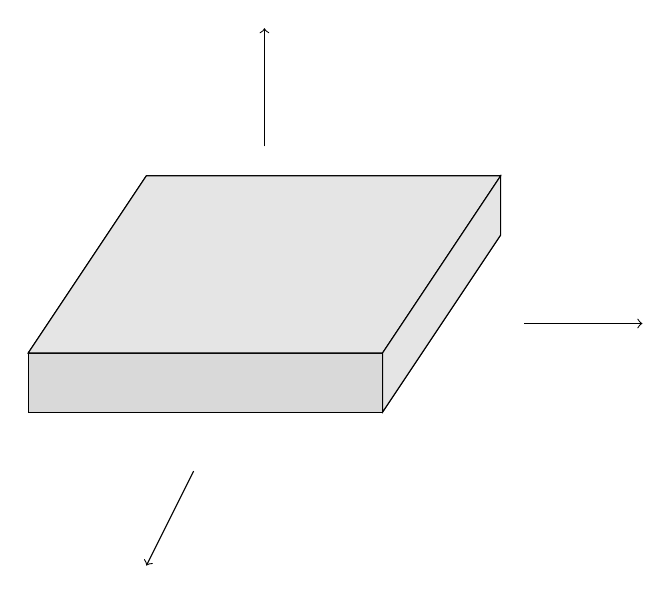
\begin{tikzpicture}[scale=1.5]
        % Face avant
        \draw[fill=gray!30] (0,0) rectangle (3,0.5);
        
        \draw (0,0.5) -- (1,2);
        \draw (3, 0.5) -- (4,2);
        \draw (3,0) -- (4,1.5);
        \draw (4,1.5) -- (4,2);
        \draw (1,2) -- (4,2);
        \draw[fill=gray!20] (0,0.5) -- (3,0.5) -- (4,2) -- (1,2) -- cycle;
        \draw[->] (2, 2.25) -- (2, 3.25);
        \draw[->] (4.2, 0.75) -- (5.2, 0.75);
        \draw[->] (1.4,- 0.5) -- (1,-1.3);
        \draw[fill=gray!20] (3,0) -- (3,0.5) -- (4,2) -- (4,1.5) -- cycle;			
    \end{tikzpicture}
    
    \captionof{figure}{LSM9DS1 axis  on this card}	
\end{center}

\subsection{Gyroscope}

The STMicroelectronics LSM9DS1 gyroscope is a  measuring instrument designed to assess rotation rates around the x, y, and z-axes. With a typical measurement range of ±245, ±500, ±2000 dps, it offers adaptability to the specific needs of the application.The gyroscope of LSM9DS1  has an acceleration sampling rate that can be modified to take the following values: 14.9 Hz, 59.5 Hz, 119 Hz, 238 Hz, 476 Hz, 952 Hz.
\bigskip

This gyroscope operates with a voltage range of 1.71 V to 3.6 V, allowing it to easily integrate into different system configurations. Furthermore, its typical operating current ranges from 1 mA to 2 mA, ensuring optimal energy efficiency for battery-powered devices.

\bigskip

Whether it's for inertial navigation, drone stabilization, or other applications requiring precise motion measurement, the gyroscope of LSM9DS1  delivers reliable and accurate performance in a compact and robust form factor, meeting the highest requirements of engineers and designers.

\begin{center}
    
    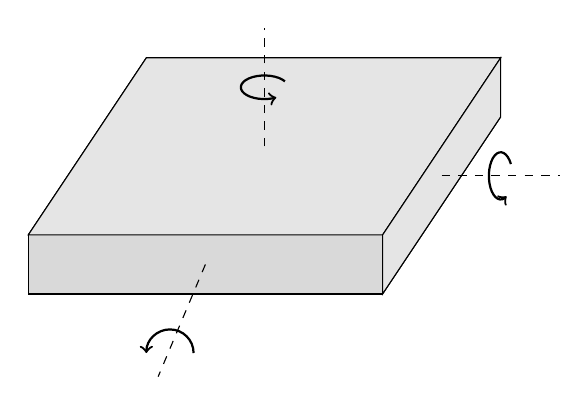
\begin{tikzpicture}[scale=1.5]
        % Face avant
        \draw[fill=gray!30] (0,0) rectangle (3,0.5);
        
        \draw (0,0.5) -- (1,2);
        \draw (3, 0.5) -- (4,2);
        \draw (3,0) -- (4,1.5);
        \draw (4,1.5) -- (4,2);
        \draw (1,2) -- (4,2);
        \draw[fill=gray!20] (0,0.5) -- (3,0.5) -- (4,2) -- (1,2) -- cycle;
        \draw[fill=gray!20] (3,0) -- (3,0.5) -- (4,2) -- (4,1.5) -- cycle;
        \draw[dashed] (2, 1.25) -- (2, 2.25);
        \draw[dashed] (3.5, 1) -- (4.5,1);
        \draw[dashed] (1.5,0.25) -- (1.1,-0.7);
        \draw[thick, ->] (1.4,-0.5) arc[start angle=0,end angle=180,radius=0.2];
        \draw [black, thick, domain=30:300, ->] plot ({2+0.2*cos(\x)}, {1.75+0.1*sin(\x)});
        \draw [black, thick, domain=30:300, ->] plot ({4+0.1*cos(\x)}, {1+0.2*sin(\x)});
    \end{tikzpicture}
    
    \captionof{figure}{LSM9DS1 axis  on this card}
    
    
\end{center}

\section{Specification}

\subsection{Accelerometer Sensor}

The accelerometer is composed by sensor type MEMS (Micro-Electro-Mechanical Systems) and they used microscopic structures like suspended beams or springs, which deform in response to acceleration. The deformation of these structures is measured using displacement sensors or changes in electrical resistance. MEMS accelerometers are commonly used due to their small size, low power consumption, and comparatively lower cost compared to other types of accelerometers.

\bigskip 

The Accelerometer sensor function by : 

\begin{itemize}
    \item Acceleration Integration for Velocity Estimation: To estimate velocity, the acceleration measured by the accelerometer is integrated over time. Integrating acceleration over time yields velocity.
    
    \item Error Compensation: However, it's crucial to note that acceleration integration is susceptible to cumulative errors. Errors stemming from sensor noise, drift, and inaccuracies can accumulate over time, leading to inaccurate or biased velocity estimates.
    
    \item Utilization of Filters and Sensor Fusion Techniques: To compensate for these errors, advanced techniques such as Kalman filters, Complementary filters, or sensor fusion techniques can be employed. These techniques combine accelerometer data with other sensors such as gyroscopes to enhance velocity estimation accuracy.
    
    \item Calibration and Adjustment: It's also vital to calibrate and adjust the IMU to correct systematic errors and ensure precise measurements. This may involve steps such as compensating for Earth's gravity, correcting gyroscope drift, and reducing sensor noise. 
    
\end{itemize}
\subsection{PIN Conncetion}

They are 4 ways to connect pin, ways depend of what they have after. 

\begin{itemize}
    \item Mode 1: You can utilize either the I\textsuperscript{2}C / MIPI I3CSM slave interface or the SPI (3- and 4-wire) serial interface.
    
    \item Mode 2: This mode supports both the I\textsuperscript{2}C / MIPI I3CSM slave interface or the SPI (3- and 4-wire) serial interface, along with an I\textsuperscript{2}C interface master for external sensor connections.
    
    \item Mode 3: Here, you have the choice of employing either the I\textsuperscript{2}C / MIPI I3CSM slave interface or the SPI (3- and 4-wire) serial interface for the application processor interface. Additionally, an auxiliary SPI (3- and 4-wire) serial interface is designated for external sensor connections, exclusively for the gyroscope.
    
    \item Mode 4: Similar to Mode 3, this mode offers the I\textsuperscript{2}C / MIPI I3CSM slave interface or the SPI (3- and 4-wire) serial interface for the application processor interface. Additionally, it provides an auxiliary SPI (3- and 4-wire) serial interface for external sensor connections, catering to both the accelerometer and gyroscope.	
    
\end{itemize}

\begin{center}
    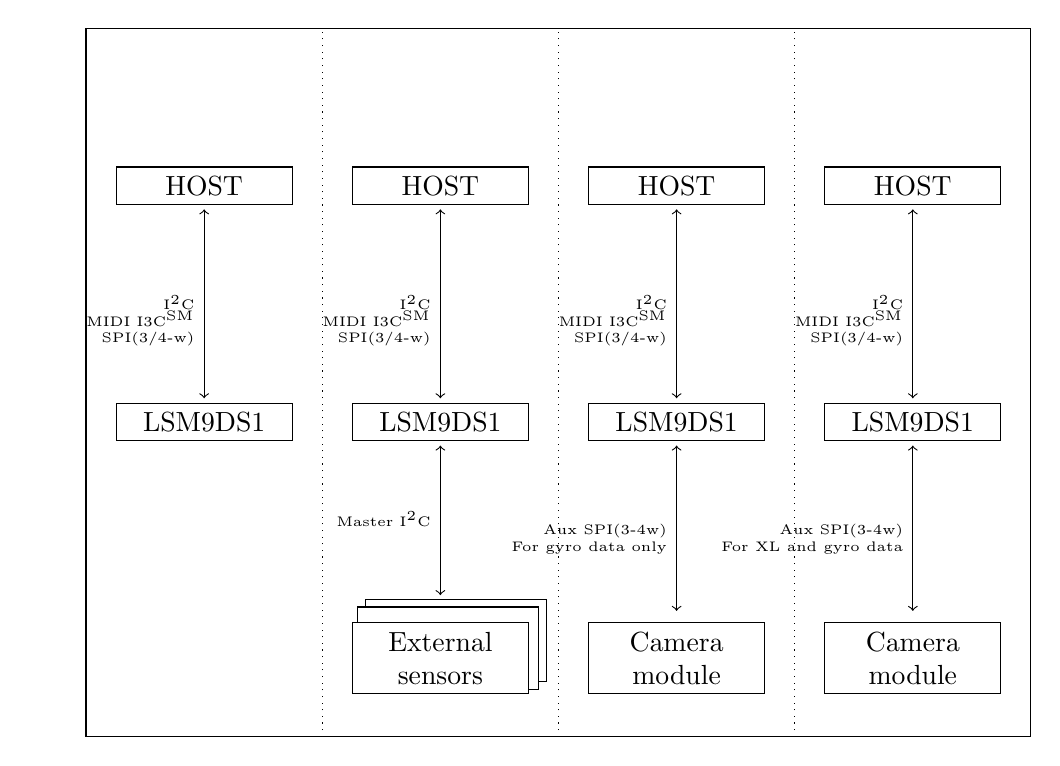
\begin{tikzpicture}
        \draw[fill=white] (0,0) rectangle++(12,9);
        \foreach \x in {3,6,9}{
            \draw[dotted] (\x, 0) -- (\x, 9);}
        \foreach \x in {1.5,4.5,7.5,10.5}{
            \node[draw, fill=white!20, text width=2cm, align=center] at (\x,7) {HOST};
            \node[draw, fill=white!20, text width=2cm, align=center] at (\x,4) {LSM9DS1};}
        \foreach \x in {1.5,4.5,7.5,10.5}{
            \draw[<->](\x,4.3) -- (\x,6.7) node[midway, anchor = mid east, align = right, text width = 2cm, font=\tiny]{I\textsuperscript{2}C\\ MIDI I3C\textsuperscript{SM}\\SPI(3/4-w)};}
        \foreach \x in {7.5,10.5}{
            \node[draw, fill=white!20, text width=2cm, align=center] at (\x,1) {Camera module};
            \draw[<->](\x,1.6) -- (\x,3.7) node[midway, anchor = mid east, align = right, text width = 2cm, font=\tiny]{Aux SPI(3-4w)};}
        \node[anchor=east, align= left, font=\tiny] at (7.5,2.4) {For gyro data only};
        \node[anchor=east,  align= left, font=\tiny] at (10.5,2.4) {For XL and gyro data};
        \draw[fill=white] (3.55,0.7) rectangle++(2.3, 1.05) ;
        \draw[fill=white] (3.45,0.6) rectangle++(2.3, 1.05) ;
        \node[draw, fill=white!20, text width=2cm, align=center] at (4.5,1) {External sensors};
        \draw[<->](4.5,1.8) -- (4.5,3.7) node[midway, anchor = mid east, align = right, text width = 2cm, font=\tiny]{Master I\textsuperscript{2}C};
        
    \end{tikzpicture}
    
    \captionof{figure}{Explication of pin mode}  
\end{center}


\section{Library}

\subsection{Library Description}

To support the project's requirements, we need 3 main libraries, each serving a specific need : 

\begin{enumerate}
    \item \FILE{Wire.h}: This library is a standard Arduino library that facilitates communication between I\textsuperscript{2}C (Inter-Integrated Circuit) devices. I\textsuperscript{2}C is a synchronous serial communication protocol used to connect microcontrollers to external devices. \FILE{Wire.h} provides functions for initializing the I\textsuperscript{2}C bus, sending and receiving data on the bus, and managing multiple devices on the same bus. With this library, developers can easily connect multiple I\textsuperscript{2}C devices, such as sensors or displays, to an Arduino board.
    
    \item \FILE{Kalman.h}: This library implements the Kalman filter algorithm. The Kalman filter is a mathematical technique used to estimate the state of a system from incomplete measurements. It is commonly used in control systems, robotics and navigation applications to improve the accuracy of sensor measurements and reduce errors. \FILE{Kalman.h} provides a simple interface for developers to implement the Kalman filter in their Arduino projects.
    
    \item \FILE{Arduino\_LSM9DS1.h}: The library \FILE{Arduino\_LSM9DS1.h} is a software library designed to facilitate interaction with the sensor accelerometer LSM9DS1, developed by STMicroelectronics. This sensor combines an accelerometer, a gyroscope and a magnetometer in a single package.The library LSM9DS1 provides an interface for accessing the sensor's functionalities, such as reading acceleration, angular velocity and magnetic field data. It can be used to configure various sensor parameters, such as measurement scales, sampling rates and operating modes.
    
    
\end{enumerate}

\subsection{Installation}

The library give some example of sketch, to use this sketch we need to download the library on ArduinoIDE. The library \FILE{Arduino LSM9DS1.h} and \FILE{Kalman.h} can be download directly on Arduino. The library \FILE{wire.h} is used if you imput :  \PYTHON{\#include <wire.h>}

\begin{center}
    \includegraphics[width = 14cm]{Arduino/IMU/wire.png}
    \captionof{figure}{Wire include } 
\end{center}


\begin{center}
    \includegraphics[width = 15cm]{Arduino/IMU/LSM6DSboard.png}
    \captionof{figure}{Board card installation}
\end{center}

\begin{center}	
    \includegraphics[width = 5cm]{Arduino/IMU/LSM9DS1.png}
    \captionof{figure}{Library choice }
\end{center}

\bigskip

\section{Function}

The library LSM9DS1 on Arduino Nano 33 BLE Sense is composed of different function. The function is different if you was on I\textsuperscript{2}C protocol or SPI protocol.

\lstdefinestyle{Arduino}{
    language=Arduino,
    basicstyle=\ttfamily\small,
    keywordstyle=\color{blue},
    stringstyle=\color{yellow!30!black},
    commentstyle=\color{green!60!blue},
    morecomment=[l]{//},
    morecomment=[s]{/*}{*/} }

\subsection{Library \FILE{Wire.h}}


This library is used to devellop communication betwin different composent of Arduino board, it's used for I\textsuperscript{2}C. The library \FILE{Wire.h} is composed by : 
\begin{itemize}
    
    \item \PYTHON{Wire.begin()}: Initializes the library \PYTHON{Wire.h} and prepares the Arduino to act as master or slave on the bus I\textsuperscript{2}C.
    \item \PYTHON{Wire.beginTransmission(address)}: Starts a transmission to a slave device with the specified address.
    \item \PYTHON{Wire.write(data)} : Sends data on the I2C bus during transmission.
    \item \PYTHON{Wire.endTransmission()} : Ends the current transmission and releases the I2C bus.
    \item \PYTHON{Wire.requestFrom(address, quantity)} : Requests data from a slave device with the specified address.
    \item \PYTHON{Wire.available()}: Checks whether data is available to be read after a request.
    \item \PYTHON{Wire.read()}: Reads data received from a slave device.
    
\end{itemize}

We can test the function with on example of the library \FILE{Wire.h}. This is an axemple to test the I\textsuperscript{2}C bus on the board. 
\begin{center}
    
    \captionof{code}{Simple sketch using the sensor LSM9DS1  detection}
    \label{TestWire}
    \ArduinoExternal{}{../../Code/Nano33BLESense/IMU/Test/WireEx.ino}
    
\end{center}
\subsection{Function \PYTHON{IMU.begin()}}


The function to initialized the IMU is \PYTHON{IMU.begin()}, they start the IMU initialization process. This step is important to configures the IMU's basic parameters, set the communications with other devices, and prepares the unit for proper operation. Accurate initialization is essential to ensure the accuracy and reliability of the data provided by the IMU.

An error during the initialization can lead to inaccurate measurements or unpredictable behavior. For example, incorrectly configured measurement parameters or sampling rates can compromise data quality, affecting overall system performance.


\begin{lstlisting}[style= Arduino]
    if (!IMU.begin()) {
        Serial.println("Failed to initialize IMU!");
        while(1){};	}
\end{lstlisting}


\subsection{Function \PYTHON{IMU.end()}} 

This function is composed without parameter. After do this function they return value of 1 if all is good and they return value of 0 if we had some problem.

This function is used to stop or deactivate the IMU once it is no longer required. It frees up the resources used by the IMU and ends its operation cleanly. When called, it ensures that all tasks associated with the IMU are properly finalized, avoiding memory leaks or other problems associated with incomplete de-initialization.

This step helps to ensure the stability and reliability of the system as a whole, by avoiding problems associated with incorrect IMU de-initialization.

The data was return at the end. 

\begin{lstlisting}[style=Arduino]
    if (!IMU.begin()) {
        Serial.println("Failed to initialize IMU!");
        while(1){}; }
\end{lstlisting}


\subsection{Function \PYTHON{IMU.readAcceleration(x,y,z) }}

The \PYTHON{IMU.readAcceleration()} is used to read the IMU accelerometer and obtain the data, this is expressed in gravity (g). This function provides information on the movements detected by the IMU's accelerometer. The resulting acceleration data can be used for a variety of applications, such as shock or motion detection, or inertial navigation. By regularly interrogating the accelerometer and analyzing variations in acceleration, it is possible to understand and react to changes in motion with precision, which is essential in many modern embedded systems and electronic devices.

The parameters x, y and z are floats giving information on the x, y or z-axis 

\begin{lstlisting}[style=Arduino]
    
    float x; 
    float y; 
    float z;
    
    if (IMU.accelerationAvailable()) {
        IMU.readAcceleration(x, y, z);
        
        Serial.print(x);
        Serial.print('\t');
        Serial.print(y);
        Serial.print('\t');
        Serial.println(z);	}
\end{lstlisting}

\subsection{Function \PYTHON{IMU.readGyroscope()}}

Retrieves data from the IMU's gyroscope and returns angular velocity in degrees per second (dps). This function provides information on the rotational movement detected by the IMU's gyroscope. The angular velocity data retrieved can be used in various applications such as robotics, motion tracking or navigation systems. By regularly interrogating the gyroscope and analyzing angular velocity variations, it becomes possible to understand and respond precisely to rotational movements, which is crucial in applications requiring precise orientation control or stabilization.

The parameters x, y and z are floats giving information on the x, y or z axis 

\begin{lstlisting}[style=Arduino]
    float x, y, z;
    
    if (IMU.gyroscopeAvailable()) {
        IMU.readGyroscope(x, y, z);
        
        Serial.print(x);
        Serial.print('\t');
        Serial.print(y);
        Serial.print('\t');
        Serial.println(z);	}
\end{lstlisting}



\subsection{Function \PYTHON{IMU.accelerationAvailable()}}

This function allows you to check the status of IMU acceleration data, indicating whether or not new data is ready to be retrieved.

In scenarios such as motion tracking, robotics or navigation systems, where the IMU continuously captures acceleration data, the availability of new data determines the system answers. Test the IMU at regular intervals is used for application and they can check for acceleration currently or non, ensuring that the system remains synchronized with object movements in real time.

When the function returns a value of 1, this means that new acceleration data is available, enabling the system to extract the data and process it further. A value of 0 indicates that there have been no recent acceleration updates.

\begin{lstlisting}[style=Arduino]
    float x, y, z;
    
    if (IMU.accelerationAvailable()) {
        IMU.readAcceleration(x, y, z);
        
        Serial.print(x);
        Serial.print('\t');
        Serial.print(y);
        Serial.print('\t');
        Serial.println(z); }
    
\end{lstlisting}


\subsection{Function \PYTHON{IMU.gyroscopeAvailable()}}

This function ask if new gyro data are available for the IMU and they returns a value 0 if no new gyro data is available, and 1 if new gyro data is ready to be retrieved.

In applications requiring real-time monitoring of rotational motion, such as drone stabilization, virtual reality systems or inertial navigation, the system can determine whether to wait for updated gyroscope readings or proceed to process available data.

A value of 1 indicates that new gyro data is available, enabling the system to retrieve and use this information for adapted the orientation tracking or motion control. Conversely, a feedback value of 0 indicates that there have been no recent updates to the gyroscope measurements, prompting the system to wait for new data to become available before proceeding.

\begin{lstlisting}[style=Arduino]
    float x, y, z;
    
    if (IMU.gyroscopeAvailable()) {
        IMU.readGyroscope(x, y, z);
        
        Serial.print(x);
        Serial.print('t');
        Serial.print(y);
        Serial.print(' t');
        Serial.println(z); }
\end{lstlisting}


\subsection{Function \PYTHON{IMU.accelerationSampleRate()}}

This function is designed to provide information on the sampling rate of the IMU's accelerometer. The function \PYTHON{IMU.accelerationSampleRate()} returns the accelerometer sampling rate, expressed in Hertz (Hz). This value represents the frequency at which the accelerometer takes measurements and provides acceleration data. It indicates how many times per second the accelerometer registers changes in acceleration along its axes.

In activities such as motion tracking, gesture recognition or vibration analysis, knowledge of the accelerometer's sampling rate ensures that the system can accurately capture and respond to changes in motion dynamics. 

\begin{lstlisting}[style=Arduino]
    Serial.print("Accelerometer sample rate = ");
    Serial.print(IMU.accelerationSampleRate());
    Serial.println(" Hz");
    Serial.println();
    Serial.println("Acceleration in g's");
    Serial.println("X \t Y  \t Z");
\end{lstlisting}



\subsection{Function \PYTHON{IMU.gyroscopeSampleRate()}}

To recover and communicate the specific rate at which the gyroscope, integrated into the inertial measurement unit (IMU), collects data samples. This frequency is usually expressed in hertz (Hz), corresponding to the number of samples acquired per second. This is the frequency at which the gyroscope takes measurements, giving an idea of its operational efficiency and performance.

\begin{lstlisting}[style=Arduino]
    Serial.print("Gyroscope sample rate = ");
    Serial.print(IMU.gyroscopeSampleRate());
    Serial.println(" Hz");
    Serial.println();
    Serial.println("Angular speed in degrees/second");
    Serial.println("X tY tZ");
    
\end{lstlisting}




}








%\Ausblenden
{

\part{Arduino Nano 33 BLE Sense - External  Sensors and Actors}

%%%
%
% $Autor: Wings $
% $Datum: 2021-05-14 $
% $Pfad: LEDExternal $
% $Dateiname: 
% $Version: 4620 $
%
% !TeX spellcheck = de_DE/GB
% !TeX program = pdflatex
% !BIB program = biber/bibtex
% !TeX encoding = utf8
%
%%%

%todo citations
%todo create tikz pictures
%todo create sketches /ino-files with the code
%todo test the code

% Farben: https://rgbcolorcode.com/color/00FF00

\chapter{External Standard LED}


\section{General}

LED stands Light-Emitting Diode. A diode is an electronic component that only allows current to pass in one direction. Most diodes are made of semiconductor materials; in the case of light-emitting diodes, it is usually silicon.

The way an \ac{led} works is known from the animal world. For example, the energetic firefly is a flying \ac{led}. The only difference is how the atoms inside are excited and thus made to glow. The fireflies achieve this through a chemical reaction. In the \ac{led}, this happens with the help of an electric current - in short: electroluminescence.

A light-emitting diode consists of an anode (positive pole) and a cathode (negative pole). A wire, the so-called bonding wire, ensures the flow of current between the two poles. The energy required for electroluminescence flows through this wire. The semiconductor crystal (also known as the \ac{led} chip) sits on the cathode. It is surrounded by a reflector trough that directs the light from the \ac{led} chip upwards. The entire structure is embedded in a protective plastic lens. It distributes the light in the room, thereby increasing both the efficiency and the luminous efficacy.

The chip is a semiconductor crystal made from two different materials that are doped differently. Doping means that there is an excess of positive or negative charge carriers. When current flows, the electrons react and energy is released in the form of light flashes (photons). The \ac{led} lights up.

The color of the light depends on the doping of the semiconductor layers. Depending on the energy level, photons with different wavelengths, i.e. light color, are released. For example, a high energy level produces short-wave blue light and a low energy level produces long-wave red light. The superposition of the three primary colors red, blue and green produces white light. The colors red and green produce yellow. Red and blue become magenta, green and blue produce cyan.

A multicolor light-emitting diode therefore contains three semiconductor crystals, each of which produces one of the three primary colors and expands the color palette in different compositions.

Depending on how the brightness of red, green and blue is controlled, white is produced in different shades between very bright cool white light (indicated on the packaging as ``5000 Kelvin'' and above) or dimmed warm feel-good light (around 3000 Kelvin). As this variant of the mixture is expensive, there is now a new manufacturing option: blue \ac{led} chips are coated with a yellowish phosphor layer.

The colors available for ac{led}s are quite diverse, ranging from the basic red, green, and blue (RGB) to a much wider spectrum depending on the technology and application. \cite{Quadrios:2020} Here's a breakdown of the different types:

\begin{description}
  \item[Red:] This is the most common LED color, achieved by using materials like gallium arsenide phosphide (GaAsP). It has a dominant wavelength around 620-750 nm and appears vibrant red to the human eye.
  \item [Green:] Another common LED color, typically made with indium gallium nitride (InGaN). Its dominant wavelength falls between 500-570 nm, producing a bright green color.
  \item [Blue:] Blue LEDs are often made with gallium nitride (GaN) and emit light with a dominant wavelength of 450-480 nm. They appear as a deep, rich blue to our eyes.
\end{description}  

\medskip
  
Combinations and White Light:

\begin{description}
   \item [White:] While not a single color, white LEDs are crucial for various applications. They are typically achieved in two ways:
     \begin{itemize}
       \item RGB combination: Combining red, green, and blue LEDs in specific ratios can create white light. This method offers flexibility in color temperature control.
       \item Phosphor conversion: A blue or ultraviolet LED is coated with a phosphor that converts part of the emitted light to longer wavelengths, generating white light. This method is more efficient but offers less color control.
     \end{itemize}
\end{description}

\medskip


Beyond the Basics:

\begin{description}
  \item [Amber:] Often used in traffic signals and indicator lights, amber LEDs have a dominant wavelength around 585-605 nm and appear yellowish-orange.
  \item [Yellow:] True yellow LEDs are less common but achievable with specific materials like aluminum gallium indium phosphide (AlGaInP). Their dominant wavelength is around 580-590 nm, appearing as a pure yellow color.
  \item [Other colors:] Specialized LEDs can produce various other colors, including violet, pink, cyan, and even deep red and green for wider spectrum applications. These often involve more complex materials and manufacturing processes.
\end{description}

It's important to note that the specific color of an ac{led} can vary slightly depending on factors like manufacturing tolerances, viewing angle, and operating conditions. Additionally, new ac{led} technologies are emerging constantly, potentially expanding the color range further in the future.
\cite{Kainka:2009, Hering:2021,Hering:2023,Baichtal:2018}




\section{Specification}    


A \ac{led} need to have a resistor placed in series with it. Otherwise, the unrestricted current will quickly burn out the \ac{led}. The resistor can be any value between 100 Ohms and about 10K Ohms. It is necessary to check the data sheet. Lower value resistors will allow more current to flow, which makes the \ac{led} brighter. Higher value resistors will restrict the current flow, which makes the \ac{led} dimmer. A typically value is 220 Ohm. Using the data sheet of the LED, the value of the resistor can be determined. \cite{Quadrios:2020,Huiyuan:2017}
The maximal current to operate an \ac{led} is 20mA. It works also using 4mA until 15 mA. \cite{Quadrios:2020}


Most \ac{led}s have polarity, which means that they need to be connected the right way around. Usually, the \ac{led}'s shortest lead connects to the ground side, see figure \ref{LED:Standard}

\begin{center}
%todo tikz picture with strip red - red - black - brown 1\%
% or red - red - black - gold 5\%
\includegraphics[width=0.8\textwidth]{Sensor/Resistor/R}
  \captionof{figure}{Resistor with 220 Ohm for an external LED.}
\end{center}


%\includegraphics[width=0.8\textwidth]{Sensor/LED/LEDDesign.jpg}

\begin{center}
%todo tikz picture  
  \includegraphics[width=0.3\textwidth]{Sensor/LED/LED.jpg}\quad
  \includegraphics[width=0.3\textwidth]{Sensor/LED/LED2.jpg}
  \captionof{figure}{Parts of a LED.}\label{LED:Standard}
\end{center}

\begin{center}
%todo tikz picture  
  \includegraphics[width=0.8\textwidth]{Sensor/LED/circuitLED}
  \captionof{figure}{Schematic Symbol for a LED.}

\end{center}  


The Arduino can control as many \ac{led}s as long as there are enough pins available. 



\section{Using Standard External LED}\index{LED!Standard LED}


\subsection{Connecting a LED to the Arduino Board}

\Mynote{create  a diagram that shows how to connect a common cathode RGB LED to the board}


\subsection{Pins}

As mentioned, the Arduino can control as many \ac{led}s as long as there are enough pins available. There two different types of output pins
The standard output pin can just switch between high and low. For some pins the \ac{pwm} is usable. Usiing such a pin, the brightness of the ac{led} can be controlled.

\Mynote{Which pins}

PWM  A0 - A7 Welche Nummer? 16-23? 19 - 26

Digital D2-D13 Welche Nummer Pin 5 -16


\Mynote{Grafik!}


\section{Bibliothek}

No special library is required to operate an external LED.



\section{Simple Code}


As soon as the ac{led} is connected, it can be used. It is not necessary to install a special library.
Programming takes place in three steps:

\begin{enumerate}
    \item In the first step, the ac{led} must be connected to a pin:
    
    {
        \captionof{code}{Defining the pin for an external LED}
        \begin{Arduino}
            #define LED_EXT 14
        \end{Arduino}
    }
    \item In the second step, the pin is configured in the function \PYTHON{setup}:
    
    {
        \captionof{code}{Defining the pin for an external LED}
        \begin{Arduino}
            pinMode(LED_EXT, OUTOUT)   
        \end{Arduino}
    }
    \item In the third step, the ac{led} can be used in the function \PYTHON{loop}. To turn OFF the \ac{led}s, write a state \PYTHON{LOW} to the \ac{led}:
    
    {
        \captionof{code}{Swichting On the LED}
        \begin{Arduino}
            // Swichting On the LED        
            digitalWrite(LED, HIGH); 
            //Waiting 1s
            delay(1000)
            // Swichting Off the LED
            digitalWrite(LED, LOW);
        \end{Arduino}
    }
    
\end{enumerate}



\section{Tests}

\subsection{Simple Function Test}

The simplest test is the flashing of the LED at 2 Hz, see sketch \ref{Nano:LEDTest}.

{
    \captionof{code}{Simple sketch to test a LED}\label{Nano:LEDTest}
    \ArduinoExternal{}{../../Code/Nano33BLESense/Test/TestLED.ino}
}



\subsection{Test all Functions}

Standard pins can be used, but pins that support pulse width modulation can also be used. One such pin is used in the example \ref{Nano:TestLEDPWM}. The brightness can then be varied.

{
    \captionof{code}{Simple sketch to test a LED with pulse width modulation}\label{Nano:TestLEDPWM}
    \ArduinoExternal{}{../../Code/Nano33BLESense/Test/TestLEDBrightness.ino}
}



%%%%%%%%%%%%%%%%%%%%%%%%%%%%%%%%%%%%%

\section{Simple Application}

In the sketch \ref{Nano:TestLEDInterrupt}, a variable is connected to pin 14.\index{Pin!Pin 14} The pin is defined as an output in the function \PYTHON{setup}.
An interrupt function is defined, changing the state of a flag. If the flag has the value \PYTHON{true}, the led is switch on for 2 seconds. After the 2 seconds, the led is switch off and the value of the flag is set to \PYTHON{false} back.


{
    \captionof{code}{Simple sketch to control an external  LED. Here, pushing the built-in button is handled by an interrupt. Then the LED switch on for 2 sec.}\label{Nano:TestLEDInterrupt}
    \ArduinoExternal{}{../../Code/Nano33BLESense/Test/TestPushButtonInterrupt.ino}
}

\bigskip

This is just a simple example. The variable \PYTHON{BUTTON\_B} is already defined, so the assignment is not necessary. The command \PYTHON{delay} should be avoided in an Arduino sketch. Instead, variables of the type \PYTHON{elapsedMillis} should be used.


\section{Further Readings}


\Mynote{citations}











%%%
%
% $Autor: Wings $
% $Datum: 2021-05-14 $
% $Pfad: LEDRGBExternal $
% $Dateiname: 
% $Version: 4620 $
%
% !TeX spellcheck = de_DE/GB
% !TeX program = pdflatex
% !BIB program = biber/bibtex
% !TeX encoding = utf8
%
%%%

%todo citations
%todo create tikz pictures
%todo create sketches /ino-files with the code
%todo test the code


% Farben: https://rgbcolorcode.com/color/00FF00

\chapter{External RGB-LED}


\section{Standard RGB-LED}\index{LED!Standard RGB-LED}

An RGB-LED is a type of \ac{led} that can emit different colors of light. RGB stands for red, green, and blue, which are the three primary colors of light. An RGB-LED consists of three individual \ac{led}s inside a single package, each with its own color and pin. By varying the brightness of each \ac{led} using \ac{pwm} signals, an RGB-LED can produce a wide range of colors by mixing the primary colors. An RGB-LED is usually active-low, which means that setting the pin to LOW will turn the \ac{led} on, and setting the pin to HIGH will turn the \ac{led} off. 


To connect a RGB-LED to an Arduino Nano 33 BLE Sense board, you need to use three resistors, one for each color pin. The value of the resistors depends on the type and specifications of the RGB \ac{led}, but a common value is 220 ohms. You also need to connect the common cathode or anode of the RGB-LED to the ground or 3.3V pin of the board, respectively. Here is a diagram that shows how to connect a common cathode RGB \ac{led} to the board:


\Mynote{create  a diagram that shows how to connect a common cathode RGB-LED to the board}




\begin{center}
    %todo tikz picture with strip red - red - black - brown 1\%
    % or red - red - black - gold 5\%
    \includegraphics[width=0.8\textwidth]{Sensor/LED/RGB}
    \captionof{figure}{External RGB-LED with Resistors \cite{Simac:2020}}
\end{center}


External RGB-LED with Resistors \cite{Simac:2020,Kingbright:2010}



\includegraphics[width=0.8\textwidth]{Arduino/Nano33BLE/arduino-nano-33-ble-sense-pinout-1024x805.png}


\begin{center}
  %todo tikz picture on RGB-LED 
  \includegraphics[width=0.8\textwidth]{Sensor/LED/RGB-LEDs-Pinout.png}
  \captionof{figure}{Connectors of a RGB-LED.}
\end{center}


\section{Specific Sensor}

\Mynote{take a LED or RGB-LED}

\Mynote{citation}




\subsection{Pins}

Here, you can define some pins for \ac{led}s. 

\Mynote{Which one}

This must be observed when using the pins.



\begin{description}
    \item [Red LED:] LEDR = Pin 22
    \item [Green LED:] LEDG = Pin 23
    \item [Blue LED:] LEDB = Pin 24
\end{description}



\section{Specification}

cite data sheet


\section{Calibration}

cite method

\section{Simple Code}


\section{Simple Application}

\section{Tests}

\subsection{Simple Function Test}


To turn ON the \ac{led}s, write a state \PYTHON{HIGH} to the \ac{led}:



\medskip

{
    \begin{Arduino}
        digitalWrite(LEDR, HIGH); //RED
        digitalWrite(LEDG, HIGH); //GREEN
        digitalWrite(LEDB, HIGH); //BLUE
    \end{Arduino}
    \captionof{code}{Swichting On the LEDs}
}

\medskip

To turn OFF the \ac{led}s, write a state \PYTHON{LOW} to the \ac{led}:

\medskip

{
    \begin{Arduino}
        digitalWrite(LEDR, LOW); //RED
        digitalWrite(LEDG, LOW); //GREEN
        digitalWrite(LEDB, LOW); //BLUE
    \end{Arduino}
    \captionof{code}{Swichting Off the LEDs}
}

\bigskip


\subsection{Test all Functions}


\subsection{Brightness of the RGB-LED}\index{LED!Brightness}

In a short cut, using values between 255 - 0 to write to the RGB-LED is possible, too. Then the brightness is defined.

\medskip

{
    \begin{Arduino}
        analogWrite(LEDR, 72);  //GREEN 
        analogWrite(LEDG, 122); //BLUE 
        analogWrite(LEDB, 234); //RED
    \end{Arduino}
    \captionof{code}{value between 255 - 0 to write to the RGB-LED}
}

\bigskip

This sketch \ref{ArduinoLEDBrightness} will make the RGB-LED change colors smoothly by varying the brightness of each \ac{led} with different speeds. You can adjust the initial brightness values and the increment/decrement values to get different effects.

{
    \begin{Arduino}
// Define the pins for the RGB-LED
#define RED_PIN 22
#define GREEN_PIN 23
#define BLUE_PIN 24
        
// Define the initial brightness values for each color (0-255)
int redBrightness = 0;
int greenBrightness = 0;
int blueBrightness = 0;
        
// Define the increment/decrement value for each color
int redStep = 5;
int greenStep = 3;
int blueStep = 7;
        
void setup() {
    // Set the LED pins as outputs
    pinMode(RED_PIN, OUTPUT);
    pinMode(GREEN_PIN, OUTPUT);
    pinMode(BLUE_PIN, OUTPUT);
}
        
void loop() {
    // Write the PWM values to the LED pins
    analogWrite(RED_PIN, redBrightness);
    analogWrite(GREEN_PIN, greenBrightness);
    analogWrite(BLUE_PIN, blueBrightness);
            
    // Update the brightness values for each color
    redBrightness += redStep;
    greenBrightness += greenStep;
    blueBrightness += blueStep;
            
    // Check if the brightness values are out of range and reverse the direction
    if (redBrightness <= 0 || redBrightness >= 255) {
        redStep = -redStep;
    }
    if (greenBrightness <= 0 || greenBrightness >= 255) {
        greenStep = -greenStep;
    }
    if (blueBrightness <= 0 || blueBrightness >= 255) {
        blueStep = -blueStep;
    }
                    
    // Wait for 10 milliseconds
    delay(10);
}
  \end{Arduino}
  \captionof{code}{Different brightness levels for the RGB-LED colors}\label{ArduinoLEDBrightness}
}
        
  \bigskip
        
        
\subsubsection{Colors}\index{LED!Colors}
        
        A RGB-LED is a device that can emit light of different colors by mixing the primary colors of red, green, and blue. The color of the light depends on the relative brightness of each \ac{led}, which can be controlled by \ac{pwm} signals. By varying the brightness of each \ac{led}, the RGB-LED can produce a wide range of colors, such as yellow, cyan, magenta, white, and more. Some examples of the colors and their corresponding brightness values are:
        
        \begin{description}
            \item [Red:] red = 255, green = 0, blue = 0
            \item [Green:] red = 0, green = 255, blue = 0
            \item [Blue:] red = 0, green = 0, blue = 255
            \item [Yellow:] red = 255, green = 255, blue = 0
            \item [Cyan:] red = 0, green = 255, blue = 255
            \item [Magenta:] red = 255, green = 0, blue = 255
            \item [White:] red = 255, green = 255, blue = 255
            \item [Black:] red = 0, green = 0, blue = 0
        \end{description}
        
        \medskip
        
        The RGB-LED can also create intermediate colors by using different brightness values for each \ac{led}. For example, to create
        
        \begin{itemize}
            \item \textbf{orange}, one can use red = 255, green = 127, blue = 0. 
            \item To create \textbf{pink}, one can use red = 255, green = 192, blue = 203. 
            \item To create \textbf{purple}, one can use red = 128, green = 0, blue = 128. 
        \end{itemize}
        
        \medskip
        
        The RGB-LED can also create gradients of colors by changing the brightness values gradually over time. This can create a smooth transition from one color to another, such as from red to green to blue and back to red.


\section{Simple Application}


\section{Further Readings}




%%%%%%%%%%%%%%%
%
% $Autor: Wings $
% $Datum: 2020-01-29 07:55:27Z $
% $Pfad: General/SensorBME280.tex
% $Version: 1785 $
%
%
%%%%%%%%%%%%%%%

%todo   url       = {https://lastminuteengineers.com/bme280-arduino-tutorial/},


	
\chapter{Sensor BME280 für Temperatur, Luftfeuchtigkeit und den Luftdruck}

\section{Beschreibung der Hardware}

Der BME280 ist ein Temperatursensor, der von Bosch Sensortec entwickelt wurde. Der Sensor bietet die Möglichkeit, die Temperatur, Luftfeuchtigkeit und den Luftdruck in der Umgebung zu messen, siehe Abbildung \ref{fig:SensorBME280}). \cite{FunduinoBME280:2023}

\begin{figure}[h]
    \includegraphics[width=\textwidth]{Sensor/BMEsensor}
    \caption{Sensor BME280}   \cite{LastMinuteEngineers:2023}
    \centering   \label{fig:SensorBME280}
\end{figure}

Bei dem BME280 handelt es sich um einen kombinierten Sensor für die Messung von Feuchtigkeit, Luftdruck und Temperatur. Dieser ist auf dem Entwicklerboard DEBO BME280 verbaut. Das Entwicklerboard hat die Maße 15,3 x 11,5 x 2,5 mm (LxBxH), wobei der Sensor BME280 die Maße 2,5 x 2,5 x 0,93 mm (LxBxH) aufweist. Die Schnittstellen I2C und SPI des Entwicklerboards ermöglichen die Kommunikation zwischen dem Arduino und dem Sensor. Die Versorgungsspannung bewegt sich zwischen 1,72 V und 3,6 V. Die gemessene Luftfeuchtigkeit erfolgt mit einer Genauigkeitstoleranz von $\pm 3$ Prozent relativer Luftfeuchtigkeit und einer Reaktionszeit von einer Sekunde. Der Druckbereich für den Luftdruck beträgt 300 bis 1100 hPa mit einer relativen Genauigkeit von $\pm 0.12$ hPa und einer absoluten Genauigkeiten von $\pm 1$ hPa. Der Temperatursensor hat einen Bereich von -40 bis +85 °C und besitzt eine voll Genauigkeit im Bereich von $0^\circ$ bis $65^\circ$ C. Der durchschnittliche Stromverbrauch des Sensors bei einer Frequenz von 1 Hz beträgt $1.8 \mu$A für die Messung von Feuchtigkeit und Temperatur, $2.8\mu$A für die Messung von Luftdruck und Temperatur und $3.6\mu$A für die Messung von Feuchtigkeit, Luftdruck und Temperatur. Der Sensor BME280 verfügt über mehrere Pins, die für verschiedene Zwecke verwendet werden. Hierbei ist es wichtig die richtige Pin-Belegung für den Sensor zu kennen. Im Allgemeinen sind die Pins wie folgt belegt: Der VCC-Pin wird mit der positiven Stromversorgung (+3.3 V oder +5 V) des Systems verbunden. Der GND-Pin muss mit dem Masseanschluss (GND) Ihres Systems verbunden werden. Der SDA-Pin ist der Datenpin für die Kommunikation I2C. Dieser wird mit dem entsprechenden SDA-Pin auf dem Mikrocontroller verbunden. Der SCL-Pin ist der Takt-/Clock-Pin für die Kommunikation I2C. Dieser muss mit dem entsprechenden SCL-Pin auf dem Mikrocontroller verbunden werden. SDI sorgt für die SPI-Kommunikation. \cite{Bosch:2015,Bosch:2021}


\section{Schaltplan des Aufbaus}

Der folgende Schaltplan stellt die Komponenten des Arduino Nano BLE Sense Lite, des Sensors BME280 und des OLED-Displays dar. Als Spannungsquelle dient ein Computer, der den Arduino Nano 33 BLE Sense über ein USB-A auf Mikro-USB Kabel versorgt. Die Komponenten sind sinngemäß miteinander verbunden und in Abbildung~\ref{fig:Schaltplan} abgebildet.

\begin{figure}[h]
    \centering
    \includegraphics[width=0.5\textwidth] {Sensor/BMECircuit}
    \caption{Stationärer Aufbau der Wetterstation}
    \label{fig:Schaltplan} \cite{ArduinoNano33Manual:2022}
\end{figure}

\subsection{Bibliothek \FILE{cactus\_io\_BME280} für den Sensor BME280}

Die Bibliothek \FILE{cactus\_io\_BME280\_I2C} ist eine spezielle Arduino Bibliothek zur Kommunikation mit dem Sensor BME280. Die Bibliothek erleichtert die Interaktion mit dem Sensor BME280 und bietet eine einfache Möglichkeit, Messwerte abzurufen und sie in Ihren Arduino-Projekten zu verwenden. Um die Bibliothek \FILE{cactus\_io\_BME280\_I2C} zu verwenden, muss sie erst als ZIP-Datei heruntergeladen und anschließend von dem Arduino Library Manager installiert werden. Mit Hilfe von \PYTHON{\#include<"cactus\_io\_BME280\_I2C">} können diese in dem Arduino-Code eingebunden werden. \cite{IotSpace:2020}

\subsection{Testen des OLED-Displays}

Für die Programmierung des Displays gibt es viele Möglichkeiten. Da es viele Librarys gibt, muss zuerst einmal überlegt werden, welche verwendet werden sollen. Um einen ersten Eindruck über die Programmierung des Displays zu bekommen, wurde zunächst ein Beispielsketch getestet. Es handelt sich hier um den Sketch ``Hello World'', welcher unter \FILE{Datei -> SSD1206Ascii -> HelloWorldWire} zu finden ist (siehe Abbildung~\ref{fig:TestprogrammDisplay}).

\begin{figure}
  \includegraphics[width=1\textwidth]{OLED/TestprogrammDisplay}
  \caption{Pfad des Testprogramms.}
  \label{fig:TestprogrammDisplay}
\end{figure}

Das Testprogramm ``Hello World''(siehe Seite \pageref{Test1}) wird dafür benutzt, um den Text Hello World auf dem Display auszugeben (siehe Abbildung \ref{fig:ErsteAusgabeDisplay}). Es wird hier verwendet, um sich mit der Software vertraut zu machen und um sicherzustellen, dass die Entwicklungsumgebung richtig eingerichtet ist. Außerdem wird getestet, ob das Programmieren funktioniert und alle Kabel richtig angesteckt sind.

\bigskip

\begin{code}
\begin{Arduino}
#include <Wire.h>
#include ``SSD1306Ascii.h''
#include ``SSD1306AsciiWire.h''
#define I2C_ADDRESS 0x3c

SSD1306AsciiWire oled;

void setup() 
{
  Wire.begin();
  Wire.setClock(400000L);
  oled.begin(\&Adafruit128x64, I2C\_ADDRESS);
}

void loop()
{
  oled.setFont(System5x7);
  oled.clear();
  oled.println(``Viel'');
  oled.print(``Erfolg!!!'');
  delay(2000);
}
\end{Arduino}\label{Test1}
  \caption{Testprogramm für ein OLED-Display}
\end{code}


Nachdem der Quellcode kompiliert und an den Arduino geschickt wurde, wurde auf dem Display der Text Viel Erfolg ausgegeben (siehe Abbildung \ref{fig:ErsteAusgabeDisplay}). Hiermit ist sichergestellt worden, dass die Entwicklungsumgebung und der Compiler korrekt funktionieren. \Mynote{citation}

\begin{figure}
  \centering
  \includegraphics[width=0.5\textwidth] {OLED/Output}
  \caption{Erste Ausgabe Display} 
  \label{fig:ErsteAusgabeDisplay} \Mynote{citation}
\end{figure}



%%%%%%%%%%%%%%%
%
% $Autor: Wings $
% $Datum: 2020-01-29 07:55:27Z $
% $Pfad: General/ServoDrive.tex
% $Version: 1785 $
%
%
%%%%%%%%%%%%%%%

	
\chapter{Servomotor JAMRA 033212}

\Mynote{Ausfühtlicher!\\ Arduino-Programm? Genauigkeit?}



Elektromotoren besitzen bei geringen Drehzahlen eine geringe Kraftentfaltung. Um Platz zu sparen, werden deshalb Getriebe verwendet. Die hohe Motordrehzahl wird in ein langsames, aber hohes Drehmoment übersetzt. Dadurch bekommen Servomotoren ihre besonderen Eigenschaften: Sehr genaue Positions- und Geschwindigkeitsregelung. \cite{Bernstein:2018} 

\bigskip

Unterteilt werden Servomotoren in zwei Kategorien: Open Loop und Closed Loop. Der Open Loop-Motor hat keine Begrenzung im Drehwinkel und kann sich um $360^\circ$ frei drehen. Dieser wird auch als Schrittmotor bezeichnet. Die realisierte Anwendung zur Sonnennachführung benötigt jedoch keine volle Kreisbahn, weshalb der ausgewählte Motor in die Kategorie Closed Loop fällt. Die in der Industrie eingesetzten Servomotoren besitzen nicht zwingend ein Getriebe, sind daher deutlich größer als ein Modellbauservo. Basierend auf einem Brushless-Motor ist Magnet und Spule sehr groß ausgelegt, um die Kräfte aufzubauen. \Mynote{Quelle fehlt!} 

\bigskip

Bei dem verwendeten Servomotor ist das Chassis aus eingefärbtem, durchsichtigem Kunststoff gefertigt, weshalb ein Blick den Aufbau und die wesentlichen Bauteile zeigt.

\begin{figure}
    \begin{flushleft}
        \includegraphics[width=10cm]{Drive/Servomotor}
        \caption{Aufbau eines Servomotors \href{https://a.pololu-files.com/picture/0J3188.450.jpg?8db0bf79b0d26db613e6730cedbc62f7}{Quelle}}
        \Mynote{Eigene Beschriftung mit overpic}
    \end{flushleft}
\end{figure}



\begin{description}
  \item[Motor:] Als Aktuator ist im JAMRA 033212 ein Gleichstrommotor verbaut. Da der Motor in der Baugruppe das schwerste Bauteil ist, muss je nach Anwendung aus Einsatzzweck und Realisierung durch Getriebe und Motor ein korrektes Verhältnis abgeleitet werden. In der Sonnennachführung verläuft die Hauptlast vertikal nach unten und wird dort gelagert. Der Servomotor muss also nur ein vergleichsweise geringes Drehmoment aufbringen.

  \item[Getriebe:] Um bei kleinen Motoren das notwendige Drehmoment aufzubringen, wird ein mehrstufiges Getriebe mit hoher Untersetzung eingesetzt. Bei hochwertigen, teuren Servomotoren besteht das Getriebe aus Metallzahnrädern und ist kugelgelagert, der vorhandene Servomotor besitzt ein kostensparendes Kunststoffgetriebe.

  \item[Positionssensor:] Bei dem Servomotor ist an der Ausgangswelle ein Potentiometer angebracht. Ein Potentiometer ist ein verstellbarer Widerstand welcher als Spannungsteiler ausgelegt ist.  Bei Drehung der Welle um einen bestimmten Winkel wird der Widerstand des Potentiometers verändert. Das mittlere Anschlussbein ist der Wischer, welcher am Schleifring entlang schleift. 

  \item [Motorsteuerung:] In der Motor Steuerung kommen Spannung, Position und externes Steuersignal zusammen. Geregelt wird abhängig von der Last die Spannung und von der externen Steuerung die Position. Unterschiede gibt es in Analog- und Digitaler Steuerung. Bei der digitalen Steuerung ist ein zusätzlicher Mikrocontroller verbaut welcher die Position exakter anfahren und halten kann. Dieser ist jedoch auch teurer, weshalb wir uns für die analoge Ausführung entschieden haben.
  
  Die Spannung aus dem Spannungsteiler (Potentiometer) wird mit der Spannung aus dem Impulswandler verglichen. Aus dem Impulswandler kommt das veränderte Signal vom Arduino. Das Signal vom Arduino kommt über eine Signalleitung mit 50 Hz. Je nachdem wie breit das Signal ist, kann die Winkelstellung durch den Motor Treiber verändert werden. Die Änderung der Signalbreite wird auch als Puls Weiten Modulation bezeichnet, kurz PWM. \cite{Dejan:2018,Ibrahim:2018}
  
  Dadurch ist es möglich den Servomotor mit nur einer Steuerleitung anzusteuern. Bei steigender Spannung erhöht sich das Impulssignal bei gleichbleibender Breite. Der Servomotor ändert mit höherer Spannung seine Position schneller und auch die Stellkraft steigt. Beim Halten der Position ist der Stromverbrauch sehr gering, weshalb Servomotoren auch als Verstelleinheit eingesetzt werden.

  \begin{figure}
    \begin{center}
        \includegraphics[width=14cm]{Drive/ServoPMW}
        \caption{PWM am Servomotor \href{https://howtomechatronics.com/wp-content/uploads/2018/03/RC-Servo-Motor-Control-Signal-768x485.png?ezimgfmt=ng:webp/ngcb2}{Quelle}}
    \end{center}\Mynote{keine geeignete Quelle, richtig zitieren; eigene Zeichnung moit tikz}
  \end{figure}

\end{description}


\section{Datenblatt JAMRA 033212} 

Die Zusatzbezeichnung 9g bezieht sich auf das Eigengewicht, welches ungefähr 9 Gramm beträgt und die Bauklasse kennzeichnet. Zum Beispiel im Flugzeugmodellbau als Klappen-oder Fahrwerkssteuerung. Wichtig ist für die Anwendung vor allem die Stellkraft. Im Vorfeld muss die aufzubringende Kraft bekannt sein, um einen Passenden Servomotor auszuwählen. Am Datenblatt wird nochmal deutlich was bei steigender Spannung passiert. Die Kraft und die Geschwindigkeit nehmen zu. Den einfachen, günstigen Servomotor erkennt man auch am Kunststoffgetriebe und an fehlenden Kugellagern.

\begin{figure}
  \begin{center}
    \includegraphics[width=12cm]{Drive/ServoDataSheet}
    \caption{Auszug aus Gebrauchsanleitung JAMRA 033212, Seite 1 \cite{Jamara:2018}}
  \end{center}\Mynote{Informationen herausziehen, eigene Tabelle}
\end{figure}



\section{Schaltplan}

\begin{figure}
    \begin{center} 
        \includegraphics[width=14cm]{Drive/ServoCircuit}
        \caption{Schaltplan zum Anschluss eines Servomotors JAMRA 033212}\Mynote{Wo ist das Grove-Kabel? Motherboard?}
    \end{center} 
\end{figure}


%%%%%%%%%%%%%%%
%
% $Autor: Wings $
% $Datum: 2020-01-29 07:55:27Z $
% $Pfad: General/OLED.tex
% $Version: 1785 $
%
%
%%%%%%%%%%%%%%%

\chapter{OLED-Display}


\Mynote{Wo sind die Programmdateien?\\
Version der Bibliothek?\\
Welche Möglichkeiten?\\
Was ist OLED?\\
Funktionsbeschreibungen?\\
Grafiken?
\ldots}


\section{OLED}

Im Folgenden wird das Display  DEBO OLED2 0.96 beschrieben. Dieses kleine Display mit einem schwarzen Hintergrund und blauer Anzeigefarbe lässt sich mit I\textsuperscript{2}C ansteuern. Die hohe Auflösung bietet ein scharfes Bild.\cite{Simac:2019}

\bigskip

Technische Daten:

\begin{itemize}
  \item Auflösung: 128 $\times$ 64 Pixel
  \item Hintergrundfarbe: Schwarz
  \item Anzeigefarbe: blau
  \item Maße: 27 mm $\times$  27 mm $\times$ 11 mm
  \item Anschluss: 4-polig Anschluss
  \item Interface: I\textsuperscript{2}C
  \item SSD-Controller: SSD1306
  \item Spannungsversorgung: 3,3 - 5 V
\end{itemize}


\Mynote{Schaltbild, Anschlüsse? Stromverbrauch? Lebensdaur?\ldots}
\section{Anschluss}

In der Abbildung \ref{OLEDCurcuit} ist einer Schaltplan  zu sehen, in dem das Display verwendet wird. Die Masse des OLED-Displays ist in der Farbe schwarz gekennzeichnet und ist  über das Arduino Shield an den Masse Port des Arduino verbunden. Die  Spannungsversorgung mit 3,3V für das OLED-Display ist in rot gekennzeichnet. Die beiden Pins für die Datenübertragung und für das OLED-Display gehen in die vorgesehen SDA und SCL Pins am Arduino.
\Mynote{Farbe und Nummer?}

\begin{figure}
    \includegraphics[width=12cm]{OLED/OLEDCircuit2}
    \caption{Gesamter Schaltplan}\label{OLEDCurcuit}
\end{figure}

\Mynote{Nur Display darstellen}

\section{Programmierung}
\subsection{\textcolor{FileColor}{Wire.h}}

Die \textcolor{FileColor}{Wire.h} Bibliothek gehört nicht zu den spezielleren Bibliotheken. Trotzdem spielt sie eine wichtige funktionale Rolle, da durch sie die Verbindung zwischen dem Arduino und dem OLED-Display ermöglicht wird. \textcolor{FileColor}{Wire.h} kommt immer dann zum Einsatz, wenn eine Kommunikation über I2C erfolgen soll. Die Datenübertragung mittels I2C geschieht über die zwei Anschlüsse SDA und SCL. SDA ist eine serielle Datenübertragungsleitung und SCL sendet die erforderlichen Taktimpulse. Diese beiden Leitungen bilden in Kombination mit der Spannungsversorgung, 3V3 und GND, alle benötigten Anschlüsse, um das Display mit dem Arduino zu verbinden.   


\subsection{OLED-Display}

Das OLED-Display benötigt, wie zuvor erwähnt, die  Bibliothek SSD1306Ascii. In ihr sind jegliche Funktionen implementiert, um das Display individuell einzurichten. Mithilfe der ebenfalls herunterzuladenden Beispiele, ermöglicht man dem Anwender so einen schnellen Funktionstest. So kann beispielsweise überprüft werden, ob das Display korrekt angeschlossen ist und ob die Ausgabe funktioniert.

\begin{figure}[H]
    \centering
    \includegraphics[width=0.7\textwidth]{OLED/OLEDBibliothek}
    \caption{Beispiele in der OLED Bibliothek}
\end{figure}

\subsection{Testen des OLED-Displays}

Auf dem OLED-Display wurde das Beispiel \FILE{HelloWorldWire} geladen, um die richtige Ausgabe des Displays zu gewährleisten. Wie in Abbildung 4.4 zu sehen ist, zeigt das Display die erwartete Ausgabe an.

\begin{figure}
    \centering
    \includegraphics[width=0.9\textwidth]{OLED/OLEDTest}
    \caption{Testausgabe des OLED Display}
\end{figure}

\section{Software}

\subsection{Verwendete Bibliotheken}

Zur Ansteuerung des Displays werden folgende Bibliotheken verwendet:

\begin{itemize}
    \item \FILE{Wire.h}: Diese Bibliothek ermöglicht die Kommunikation über den I2C-Bus, der für die Ansteuerung des OLED-Displays verwendet wird \cite{ArduinoWire:2022}
    \item \FILE{Adafruit-GFX.h}: Eine Grafikbibliothek, die von Adafruit entwickelt wurde und grundlegende Funktionen zur Darstellung von Text und Grafiken auf Displays bietet \cite{AdafruitGFX:2023} 
    \item \FILE{Adafruit-SSD1306.h}: Eine Bibliothek für das  OLED-Display SSD1306, die auf der Adafruit-GFX-Bibliothek basiert\cite{ArduinoSSD:2023} \Mynote{Ist dies kompatibel? Was ist damit möglich?}
\end{itemize}

\subsection{OLED-Display}

Ein Objekt der Klasse \PYTHON{Adafruit\_SSD1306} wird erstellt, um das OLED-Display zu steuern:

\medskip

\PYTHON{Adafruit\_SSD1306 display(SCREEN\_WIDTH, SCREEN\_HEIGHT, \&Wire, -1);}

\medskip

Das Display wird mit der Auflösung 128 Pixel $\times$ 64 Pixel initialisiert:

\medskip

\PYTHON{\#define SCREEN\_WIDTH 128}

\PYTHON{\#define SCREEN\_HEIGHT 64}


\subsection{Initialisierung und Setup}
In der setup()-Methode werden die erforderlichen Initialisierungen durchgeführt:

\begin{itemize}
    \item \PYTHON{display.begin(...)}: Initialisiert das OLED-Display
    \item \PYTHON{display.clearDisplay()}: Löscht den Displayinhalt
    \item \PYTHON{display.setTextColor(WHITE)}: Setzt die Textfarbe auf Weiß
    \item \PYTHON{display.setTextSize(2)}: Setzt die Textgröße auf 2
    \item \PYTHON{pinMode(buttonPin, INPUT\_PULLUP)}: Konfiguriert den Taster-Pin als Eingang mit Pull-Up-Widerstand
    \item \PYTHON{Serial.begin(9600)}: Initialisiert die serielle Kommunikation mit einer Baudrate von 9600
    \item \PYTHON{PDM.onReceive(onPDMdata)}: Registriert den Empfang des Mikrofonsignals als PDM-Signal
\end{itemize} 

\subsection{Messungssteuerung}
Die Funktion \PYTHON{onPDMdata()} wird aufgerufen, wenn Daten vom Mikrofon verfügbar sind. Dies liest die Daten in einen Array ein und zählt die Anzahl der gelesenen Samples:

\begin{figure}[h]
    \includegraphics[width=10cm]{OLED/OLEDCode1.png}
    \caption{Code Einlesen/Zählen}
\end{figure}



Die Hauptfunktion \PYTHON{loop()} enthält zwei Funktionen für die Messungssteuerung und die Benutzeroberfläche:

\begin{figure}[h]
    \includegraphics[width=4cm]{OLED/OLEDCode2.png}
    \caption{Code Messungssteuerung}
\end{figure}


Die Funktion \PYTHON{HandleInput()} überwacht den Zustand der beiden Taster und steuert somit den Messungsablauf:

{
    \captionof{code}{Monitoring}\label{Code:OLED:Monitoring}
    \ArduinoExternal{firstline=78,lastline=127}{../../Code/Arduino/OLED/DEBO - OLED2 0.96/TestDeboOLED.ino}
}


\begin{itemize}
    \item Zunächst wird der Zustand der beiden Taster überprüft und die Abfrage nach einem gedrückten Button ist aktiv (\PYTHON{blueButtonIsPressed}, \PYTHON{redButtonIsPressed}).
    \item Wenn der blaue Taster gedrückt wird, wird die Messung gestartet, indem \PYTHON{isMeasuring} auf \PYTHON{true} gesetzt wird und die Funktion \PYTHON{StartSampling()} aufgerufen wird.
    \item Wenn der rote Taster gedrückt wird, wird die Messung beendet, indem \PYTHON{isMeasuring} auf \PYTHON{false} gesetzt wird und die Funktion \PYTHON{StopSampling()} aufgerufen wird. Je nach vorherigem Zustand des roten Tasters wird entweder der maximale Wert SPL in dB angezeigt (\PYTHON{ShowMaxdBspl()}) oder der durchschnittliche dB SPL-Wert (\PYTHON{ShowAveragedBspl()}).
    \item \PYTHON{isDelayOver} wird auf \PYTHON{true} gesetzt, wenn die Startverzögerung (definiert durch \PYTHON{measureThresholdMilliseconds}) von 1200ms abgelaufen ist.
    \item Es gibt eine kurze Verzögerung (\PYTHON{delay(50)}) zwischen den Schleifendurchläufen, um Tastenprellungen zu vermeiden.
\end{itemize} 

\subsection{Mikrofondatenverarbeitung}
Die Funktion \PYTHON{StartSampling()} initialisiert die Datenverarbeitung:

{
    \captionof{code}{Start and stop sampling}\label{Code:Mirco:StartSampling}
    \ArduinoExternal{firstline=129,lastline=138}{../../Code/Arduino/OLED/DEBO - OLED2 0.96/TestDeboOLED.ino}
}

\PYTHON{PDM.begin(1, 16000)}: Initialisiert eine Abtastrate von 16.000 Hz.
Die Funktion \PYTHON{StopSampling()} beendet die Aufnahme von Audiodaten.


\subsection{Anzeige der Ergebnisse}
Die Funktionen \PYTHON{ShowResult()} und \PYTHON{ShowMicrophoneValues()} sind für die Anzeige der Messergebnisse auf dem OLED-Display verantwortlich. \PYTHON{ShowResult()} zeigt den aktuellen SPL-Wert in dB auf dem Display an und aktualisiert den maximalen Wert SPL in dB, wenn nach der Startverzögerung ein neuer Höchstwert erreicht wird. \PYTHON{ShowMicrophoneValues()} verarbeitet die vom Mikrofon empfangenen Signale. Der maximale Samplewert wird ermittelt und verwendet, um den Wert SPL in dB zu berechnen. Die Funktion berechnet auch einen Durchschnittswert über eine bestimmte Zeit, \PYTHON{averagingTime = 200ms}, und zeigt das Ergebnis auf dem Display an. Die Funktionen \PYTHON{ShowMaxdBspl()} und \PYTHON{ShowAveragedBspl()} zeigen den maximalen bzw. den durchschnittlichen Wert SPL in dB auf dem Display an.

\subsection{Umrechnung auf den Wert dBSPL}

Die Umrechnung des Mikrofonsignals auf den dBSPL-Wert erfolgt in der Funktion \PYTHON{getDbValueFromPMC()}:

{
    \captionof{code}{Conversion of the microphone signal} \label{Code:Mirco:StartSampling}
    \ArduinoExternal{firstline=159,lastline=163}{../../Code/Arduino/OLED/DEBO - OLED2 0.96/TestDeboOLED.ino}
}


\PYTHON{MaxSampleVoltage} wird berechnet, indem der maximale Samplewert \PYTHON{maxSampleValue} mit der Referenzspannung des Mikrocontrollers („Vref = 3,3 V“) multipliziert und durch den maximalen Wert eines 16-Bit-Signed-Integers (32767) dividiert wird. 32767 ist der maximale Wert eines 16-Bit-Signed-Integers, der der maximalen Amplitude des Audiosignals entspricht.
Der dB SPL-Wert („dBspl“) wird mit der Formel „20 * log10(Voltage / Vrms) + sensitivity“ berechnet [Quelle der Fomel: PDF Decibels Formula https://physicscourses.colorado.edu/phys3330/phys3330\_sp19/resources/Decibels\_Phys\_3330.pdf University of Colorado System], wobei „Voltage“ der berechnete „maxSampleVoltage“ ist, und „sensitivity“ die Empfindlichkeit des Mikrofons in dBV (Dezibel-Volt) ist. „Vrms“ ist die RMS-Spannung (Root Mean Square), die einem Schalldruckpegel von 94 dB SPL entspricht. Dieser Wert wurde experimentell ermittelt.



\subsection{Benutzeroberfläche}
Die Funktion \PYTHON{HandleUI()} aktualisiert OLED-Display Anzeige:

{
    \captionof{code}{OLED-Aktualisierung}\label{Code:OLED:Update}
    \ArduinoExternal{firstline=227,lastline=234}{../../Code/Arduino/OLED/DEBO - OLED2 0.96/TestDeboOLED.ino}
}

\begin{figure}[h]
    \includegraphics[width=8cm]{OLED/OLEDCode7.png}
    \caption{Code }
\end{figure}

Wenn eine Messung aktiv ist („isMeasuring == true“), werden die aktuellen Messwerte auf dem Display angezeigt. Andernfalls wird der Displayinhalt aktualisiert, ohne neue Werte anzuzeigen.


\section{Das OLED-Display SSD1306}
Das OLED-Display SSD1306 dient dazu, die Messwerte des Arduinos auszugeben. Es besitzt eine Maße von ca. 27 x 27 x 4,1 mm und ist durch seinen hohen Kontrast sehr gut lesbar. Das Display besteht aus 128x64 OLED Bildpunkten, die durch den Chip SSD1306 gesteuert werden können. Das Display benötigt eine Betriebsspannung von 3,3 V bis 5 V und hat einen Stromverbrauch von 0,04 W im normalen Betrieb. Die Betriebstemperatur von -30 °C bis +80 °C sollte dabei nicht überschritten werden. Angesteuert werden kann das Display über die Schnittstelle I2C mit den Pins VCC, GND, SCL und SDA. Mit Hilfe der beiden Bibliotheken Adafruit GFX und Adafruit SSD1306 kann das Display programmiert werden. Hierzu aber mehr in dem Kapitel \label{key}
\begin{figure}[h]
    \centering
    \includegraphics[width=0.5\textwidth] {OLED/OLEDDisplay}
    \caption{Pins des OLED-Displays.}
    \label{fig:OLEDDisplay}
\end{figure}

Das Display verfügt über vier Pins, welche in der Abbildung \ref{fig:OLEDDisplay} zu sehen sind.

Der VCC-Pin, der für die Spannungsversorgung des Geräts sorgt, wird mit dem 5V-Pin des Mikrocontrollers verbunden. Der GND-Pin des Geräts wird mit dem GND-Pin des Mikrokontrollers verbunden, um eine gemeinsame Masseverbindung herzustellen. Der SDA-Pin des Geräts muss entweder mit dem speziellen SDA-Pin oberhalb des Pin 13 oder mit dem analogen Pin A4 des Mikrocontrollers verbunden werden. Der SCL-Pin des Geräts wird entweder mit dem speziellen SCL-Pin oberhalb des Pin 13 oder alternativ mit dem analogen Pin A5 des Mikrocontrollers verbunden. \cite{AZ-Delivery:2023,FunduinoOLED:2023}

\section{Schaltplan des Aufbaus}
Der folgende Schaltplan stellt die Komponenten des Arduino Nano BLE Sense Lite, des Sensors BME280 und des OLED-Displays dar. Als Spannungsquelle dient ein Computer, der den Arduino Nano 33 BLE Sense über ein USB-A auf Mikro-USB Kabel versorgt. Die Komponenten sind sinngemäß miteinander verbunden und in Abbildung \ref{fig:Schaltplan} abgebildet.

\begin{figure}[h]
    \centering
    \includegraphics[width=0.5\textwidth] {OLED/OLEDCircuit3}
    \caption{Stationärer Aufbau der Wetterstation}
    \label{fig:Schaltplan} \cite{ArduinoNano33Manual:2022}
\end{figure}

\section{Genutzte Bibliotheken}
Bei Bibliotheken handelt es sich um Ansammlungen von dem Code und Funktionen für bestimmte Anwendungen oder Hardware. Diese werden oft genutzt um Aufgaben leichter lösen zu können und ein neu schreiben von komplexen Funktionen zu vermeiden. In unserem Fall verwenden wir Bibliotheken für den Arduino, den Sensor BME280 und das OLED-Display.

\subsection{Bibliothek Wire.h}
Die Bibliothek Wire.h ist eine Standardbibliothek für Arduino-Plattformen, welche Funktionen und Methoden für die Kommunikation zur Verfügung stellt. Mit Hilfe der Schnittstelle I2C ermöglicht die Bibliothek die Kommunikation zwischen einem Arduino und einem anderen I2C-fähigen Gerät wie z.B. Sensoren oder Displays. I2C ist ein Kommunikationsbus, der im Vergleich zu seriellen Schnittstellen den Vorteil hat, dass er mit mehr als zwei Geräten kommunizieren kann. Ein I2C-Bus benötigt zwei Leitungen: SCL für ein Taktsignal und SDA für Daten.
Um die Wire.h Bibliotek anwenden zu können, muss sie am Anfang des Sketchs eingebunden werden: \textit{\#include<….h>} \cite{W3CWire:2023}


\subsection{Bibliothek SSD1306Ascii.h für das Testprogramm}
Bei der Bibliothek SSD1306Ascii.h handelt es sich um eine benutzerdefinierte Bibliothek, die ähnlich zu der Adafruit Bibliothek SSD1306 ist. Beide sind für die Ansteuerung von OLED-Displays notwendig und basieren auf den Controller-Chip SSD1306. Sie ermöglichen das einfache Schreiben von den Text, Zeichen von Formen und Anzeigen von Bitmap-Bildern auf dem Display. 
Um die Bibliothek SSD1306Ascii.h zu verwenden, muss sie erst als ZIP-Datei heruntergeladen und anschließend von dem Arduino Library Manager installiert werden. Mit Hilfe von \textit{\#include<SSD1306Ascii.h>} kann man sie in dem Arduino-Code einbinden. \cite{FunduinoBME280:2023}


\subsection{Testen des OLED-Displays }
Für die Programmierung des Displays gibt es viele Möglichkeiten. Da es viele Librarys gibt, muss zuerst einmal überlegt werden, welche verwendet werden sollen. Um einen ersten Eindruck über die Programmierung des Displays zu bekommen, wurde zunächst ein Beispielsketch getestet. Es handelt sich hier um den Sketch \FILE{Hello World}, welcher unter Datei -> SSD1206Ascii -> HelloWorldWire zu finden ist (siehe Abbildung\ref{fig:TestprogrammDisplay}).

\begin{figure}
    \centering
    \includegraphics[width=1\textwidth] {OLED/TestprogrammDisplay}
    \captionof{figure}{Pfad des Testprogramms.}
    \label{fig:TestprogrammDisplay}
\end{figure}

Das Testprogramm \FILE{Hello World} (siehe Seite \pageref{Test1}) wird dafür benutzt, um den Text Hello World auf dem Display auszugeben (siehe Abbildung \ref{fig:ErsteAusgabeDisplay}). Es wird hier verwendet, um sich mit der Software vertraut zu machen und um sicherzustellen, dass die Entwicklungsumgebung richtig eingerichtet ist. Außerdem wird getestet, ob das Programmieren funktioniert und alle Kabel richtig angesteckt sind.

\bigskip

{
    \captionof{code}{Simple program for OLED displays}\label{Code:OLED:Sample}
    \ArduinoExternal{firstline=227,lastline=234}{../../Code/Arduino/OLED/Grove - OLED Display SSD1308/TestSSD1306.ino}\label{Test1}
}


Nachdem der Quellcode kompiliert und an den Arduino geschickt wurde, wurde auf dem Display der Text Viel Erfolg ausgegeben (siehe Abbildung \ref{fig:ErsteAusgabeDisplay}). Hiermit ist sichergestellt worden, dass die Entwicklungsumgebung und der Compiler korrekt funktionieren. \cite{FunduinoBME280:2023}

\begin{figure}
    \centering
    \includegraphics[width=0.5\textwidth] {OLED/Output}
    \captionof{figure}{Erste Ausgabe Display} 
    \label{fig:ErsteAusgabeDisplay} \cite{FunduinoOLED:2023}
\end{figure}


\section{Beispiel eines  OLED-Displays}

Zur Ausgabe unserer Messwerte verwenden wir ein 0,96 Zoll OLED Display, welches über den I\textsuperscript{2}C Port mit dem Tiny Machine Learning Shield verbunden ist. Es verfügt über die Anschlüsse SDA und SCL zur Datenübertragung, über VCC zur Spannungsversorgung und GND für die Masse. Außerdem ist es mit einem internen Spannungsregler ausgestattet, der 3,3V- und 5V-Betrieb ermöglicht.

\begin{figure}[H]
    \centering
    \includegraphics[width=0.8\textwidth]{Nano33BLESense/TinyMLKit/display.jpg}
    \caption{Das Display zur Ausgabe der Messwerte}
\end{figure}
\Mynote{Quelle fehlt, Infos, \ldots}

Quelle: \HREF{https://www.reichelt.de/arduino-display-0-96-grove-oled-display-ssd1308-grv-oled-0-96-p191252.html}{Arduino - Display 0,96'', Grove OLED-Display, SSD}


\bigskip

Allgemeines

\begin{tabular}{ll}
Typ  & OLED \\
Ausführung &  Zubehör \\
Farbe  & monochrom \\
\end{tabular}
Display

\begin{tabular}{ll}
Display  & bis 1,9 Zoll \\
Diagonale  & 1,0 Zoll \\
Auflösung, physik. &  128 x 64 Pixel \\
Diagonale  & 2,44 cm \\
\end{tabular}

Ausführung
\begin{tabular}{ll}
Modell  & Arduino \\
\end{tabular}
Besonderheiten

\begin{tabular}{ll}
Besonderheit  & - \\
\end{tabular}

Sonstiges
\begin{tabular}{ll}
Spezifikation &  SSD1308 \\
\end{tabular}

Herstellerangaben

\begin{tabular}{ll}
Hersteller &  SEEED \\
Artikelnummer des Herstellers &  104030008 \\
Verpackungsgewicht  & 0.01 kg \\
\end{tabular}



\subsection{OLED}


Als weiteren Punkt werden Klassenobjekte im Header initialisiert und Adressen von Peripheriegeräten festgelegt. In diesem Fall sind es das Objekt \textit{oled} der Klasse \textit{SSD1306AsciiWire} und die Definition der Adresse des OLED-Displays. Die Adresse wurde zuvor durch einen I$^2$-Scanner bestätigt.

\begin{Arduino}		
    #define I2C_ADDRESS 0x3C  
    SSD1306AsciiWire oled;  
\end{Arduino}

Ein weiterer Punkt ist die Initialisierung und Deklarierung von globalen Variablen. Beim Farberkennungsautomaten sind es zwei Variablen. Über Pin D11, kurz 11, wird der Messtaster abgefragt. Pin D12, kurz 12, gibt bei Bedarf ein Signal an die externe RGB-LED. Durch das Voranstellen von \textit{const} werden beide Variablen zu Konstanten und könne außer über den Source-Code nicht geändert werden. Dies ergibt Sinn, da die Verkabelung sich nicht verändern wird und somit auch nicht die gewählten Pins.

\begin{Arduino}		
    const int TasterPin = 11; 
    const int LedPin = 12;   
\end{Arduino}

\subsubsection{\PYTHON{void setup}\{\}}

In der \textit{setup()}-Funktion wird zuerst die serielle Kommunikation mit einer Baudrate von 9600 bit/s gestartet. Baudrate oder auch Bitrate beschreibt die Übertragungsdauer eines Bits. Bei einer Baudrate von 9600 dauert es 104,17 \textmu s um ein Bit zu übertragen. Je höher die Baudrate ist, desto schneller wird ein Bit übertragen. Der Empfänger tastet meist mehrmals pro gesendetem Bit ab und bildet dann nach dreimaligem Abtasten den Mittelwert, welcher dann als empfangenes Bit weiterverarbeitet wird \cite{Gehrke:2022}.Nach dem Starten der seriellen Kommunikation werden die Modi der zwei genutzten Pins definiert. 

\begin{Arduino}		
    Serial.begin(9600);
    pinMode(buttonPin, INPUT);
    pinMode(ledPin, OUTPUT);
\end{Arduino}

Manche Pins können als Input oder als Output genutzt werden. Im Fall des Arduino Nano 33 BLE Sense Lite sind die Pins D13, AREF, A0-A7, TX, RX und D2-D12 als \ac{gpio} nutzbar. Über das genutzte Shield kann auf A6, A7, D11 und D12 zugegriffen werden. Genutzt werden D11 und D12. Der Tasterpin D11 wird als Input definiert um das Signal aufnehmen zu können, welches durch Drücken des Tasters ausgelöst wird. Pin D12 wird als Output definiert um die externe \ac{rgb}-\ac{led} einzuschalten. Der Befehl \textit{pinMode()} beinhaltet zusätzlich noch die Möglichkeit einen internen Pull-Up-Widerstand einzuschalten \cite{ArduinoPinMode:2019}. 



Anschließend wird das I$^2$C-Protokoll mit dem Objekt \textit{Wire} und der Funktion \textit{begin()} gestartet. Dabei wird der Arduino als Master im I$^2$C-Protokoll angemeldet\cite{ArduinoWire:2022}. Anschließend wird die Taktfrequenz mit 400kHz festgelegt \cite{ArduinoWireClock:2022}.

\begin{lstlisting}		
    Wire.begin();
    Wire.setClock(400000L);
\end{lstlisting}

Im nächsten Schritt wird das OLED-Display gestartet. Hierfür wird mit dem Objekt \textit{oled} die Funktion \textit{begin()} aufgerufen. Dieser Befehl benötigt als Funktionsparameter eine Geräteinitialisierung und die Adresse des Displays. Für die Initialisierungsphase des Farberkennungsautomaten wird ein der Text \textit{INITIALISIERUNG!} auf dem Display ausgegeben. Hierfür wird die Schriftart und die Startposition des Textes auf dem Display festgelegt \cite{ArduinoSSD:2023}.

\begin{lstlisting}		
    oled.begin(&Adafruit128x64, I2C_ADDRESS);
    oled.setFont(System5x7);
    oled.setCursor(0, 40);
    oled.println("INITIALISIERUNG!\n");
\end{lstlisting}
Der letzte Schritt in der \textit{setup()}-Funktion ist das dreimalige Blinken der externen RGB-LED. Hierfür wird eine for-Schleife genutzt. Innerhalb dieser Schleife wird die LED nach 2 s für 0,2 ms eingeschaltet und danach wieder ausgeschaltet. Anschließend wird der Bildschirm gelöscht.

\begin{lstlisting}
    for (int zaehler = 1; zaehler < 4; zaehler = zaehler + 1) {
        delay(2000);
        digitalWrite(LedPin, HIGH);
        delay(200);
        digitalWrite(LedPin, LOW);
        delay(200);
    }
    oled.clear();
\end{lstlisting}




  \InputLanguage{Contents/General/}{CAMov2640} 

%%%
%
% $Autor: Wings $
% $Datum: 2021-05-14 $
% $Pfad: Git/MLEdgeComputer/Contents/General/Camov7675 $
% $Dateiname: CAMov2640 
% $Version: 4620 $
%
% !TeX spellcheck = de_GB
%
%%%

\chapter{Sensor ov7675}

\url{https://www.arducam.com/?s=ov7675&id=98994/}

\url{https://www.arducam.com/focal-length-calculator/}

\url{https://docs.arduino.cc/tutorials/giga-r1-wifi/giga-camera/}

\URL{https://blog.arduino.cc/2020/06/24/machine-vision-with-low-cost-camera-modules/}

\URL{https://www.instructables.com/TinyML-Image-Recognition-With-Edge-Impulse-Nano-33/}


\cite{ArduCam:2024}\cite{ArduinoCam:2021b}

\section{Code}

\begin{itemize}
  \item 
  \HREF{https://www.hackster.io/umpheki/ov7670-camera-and-image-sensor-with-nano-33-ble-497c5f}{Arduino sketch} 
   \ArduinoExternalO{../../Code/Arduino/CAM/ov7675/Nano33BLEProgramToReadov7670Data.ino}     
  \item  \HREF{https://www.hackster.io/umpheki/ov7670-camera-and-image-sensor-with-nano-33-ble-497c5f}{save as png}
    \PythonExternalO{../../Code/Arduino/CAM/ov7675/ConvertRawToRGB888AndSaveAspng.py}
  \item  \HREF{https://www.hackster.io/umpheki/ov7670-camera-and-image-sensor-with-nano-33-ble-497c5f}{save as png}
\PythonExternalO{../../Code/Arduino/CAM/ov7675/ReadCameraDataFromNano33BLEViaSerial.py}
\end{itemize}
    
    

\subsection{ OV7670 Camera and Image Sensor with Nano 33 BLE}
 
source: \URL{https://www.hackster.io/umpheki/ov7670-camera-and-image-sensor-with-nano-33-ble-497c5f}

\bigskip

The OV7670 is an image sensor that can be used to capture pictures when controlled by a microprocessor such as the Nano 33 BLE. To quote the datasheet from OmniVision:

“The OV7670/OV7171 CAMERACHIP image sensor is a low voltage CMOS device that provides the full functionality of a single-chip VGA camera and image processor in a small footprint package. The OV7670/OV7171 provides full-frame, sub-sampled or windowed 8-bit images in a wide range of formats, controlled through the Serial Camera Control Bus (SCCB) interface.”

While the OV7670 is a powerful and versatile IC, it produces only Raw pixel data. For most images to be useful, they need to be in jpeg, png, tiff or similar format. This project shows how you can capture a raw image from the camera and then convert this into a png file.

Here are the major components for this project


\begin{itemize}
  \item Arduino Nano 33 BLE
  \item OV7670 camera module
  \item Breadboard
  \item Connectors
  \item Computer with Python ver 3 installed
  
\end{itemize}

\subsubsection{OV7670 CMOS VGA Sensor}

Datasheet for the OV7670 included with this project.

The block diagram from the datasheet:

\begin{center}
  \includegraphics[width=\textwidth]{CAM/ov7675/Blockdiagramm}
  \captionof{figure}{Blockdiagram, der Kamera OV7675}
\end{center}

The image array captures the arriving light and after processing the signal, the signal is converted to a digital signal in a A/D converter. This digital signal can then be read from the data bus (D0 – D7) controlled by SIO\_C and SIO\_D

The OV7670 is capable of capturing video in addition to still images. This project will focus on still images only.

The output formats available from the OV7670 are given on the first page of the datasheet. In this project, the format used is RGB565 (more explanation later)

The image array can take pictures up to 640 x 480 pixels definition. Because of memory limitations on the Nano 33 BLE, pictures up to 320 x 240 are possible (QVGA)

The specific module used in this project includes a simple lens that focuses light on the CMOS array, the focal length of which can be manually adjusted. Loosen the small set screw and twist the lens.


\begin{center}
    \includegraphics[width=\textwidth]{CAM/ov7675/CameraModule}
    \captionof{figure}{Camera Module OV7675}
\end{center}


\subsection{Connection}

Connection between the Nano and OV7670 as follows

\begin{center}
    \includegraphics[width=\textwidth]{CAM/ov7675/ConnectionTable}
    \captionof{figure}{Connection Table of the Camera Module OV7675}
\end{center}
    
    
Completing this connection is a little tricky and results in a tangle of wires. Picture included of the final connection

\begin{center}
    \includegraphics[width=\textwidth]{CAM/ov7675/CameraConnected}
    \captionof{figure}{Camera Module OV7675 connected to the Arduino Nano 33 BLE Sense}
\end{center}
    
    
RGB Formats
In this project, the RGB565 raw format will be used.

If you are interested in a complete explanation of all possible formats, consult the Wikipedia article:

\URL{https://en.wikipedia.org/wiki/List_of_monochrome_and_RGB_color_formats}

Or read this article:

\URL{https://support.touchgfx.com/docs/basic-concepts/color-formats}

RGB565 uses a total of 16 bits as shown    
    
\begin{center}
    \includegraphics[width=\textwidth]{CAM/ov7675/RGB565}
    \captionof{figure}{RGB565}
\end{center}
    
Green is allocated 6 bits because the human eye is more sensitive to graduations in green than red or blue.

This format was used in the early days of computing when processing and memory was at a premium. Most systems today use RGB888, where each color is allocated 8 bits for a total of 24 bits (so called true color).

This project requires the RGB565 format to be converted to RGB888 format. This is done by a combination of bit shifting and binary masking. The formula to achieve the conversion below:

p = original 16 bit raw 565 pixel information

red component of RGB888 = r = (p >> 11 \& 0b00011111) << 3

green component of RGB888 = g = (p >> 5 \& 0b00111111) << 2

blue component of RGB888 = b = (p >> 0 \& 0b00011111) << 3

To show a specific example, assume a pixel in RGB565 representation which is only red:

p = 11111000 00000000

right shift 11 bits p = 00000000 00011111

bit mask with 0b00011111 p = 00000000 00011111

left shift 3 and drop leading eight bits r = 11111000

Note that the result is not 100\% accurate because low information content cannot be converted to high information content. (However, high information content can always be converted to low information content.)

\subsection{Arduino OV7670 library}
    Before using the OV7670, the Arduino library must be installed.
    
    For Arduino IDE 2.x, search for OV7670 and install the library    
    
\begin{center}
    \includegraphics[width=\textwidth]{CAM/ov7675/ArduinoLib}
    \captionof{figure}{Installtion of the Arduino Library}
\end{center}

\subsection{Testing the OV7670}
        
The python program used to read data from the Nano 33 BLE requires that the python library pySerial be installed. This can be installed with the command

\SHELL{pip install pyserial }

(or sudo pip install pyserial, depending on how your computer is configured)

To check if the library is installed use

\SHELL{pip show pyserial}

To test the OV7670, two programs are required. Here are the steps:

\begin{enumerate}
  \item Upload the program “RawCameraCapture.ino” to the Nano 33 BLE
  \item Close the Arduino IDE; the serial monitor in the IDE prevents the python program from communicating with the Nano
  \item Place the camera to point at the subject. Some experimentation with lighting and distance from subject may be required
  \item Navigate to the directory containing the Python program “ReadCamera2.py”
  \item Run the the program with the command
  
        \SHELL{python3 ReadCamera2.py}
  \item Once the process is finished, a message “image transfer complete” will print in the terminal
  \item The program creates a file called “camera” which contains the raw pixel data
  \item Navigate to the website \URL{http://rawpixels.net} in a browser
  \item Upload the file \FILE{camera}
  \item Settings as follows:
    \begin{itemize}
      \item width: 176
      \item height: 144
      \item offset: 0
      \item Predefined Format: RGB565
      \item Pixel Format: RGBA
      \item Ignore Alpha checked
      \item Little Endian not checked
    \end{itemize}
\end{enumerate}

\begin{center}
    \includegraphics[width=\textwidth]{CAM/ov7675/RawPixelNet}
    \captionof{figure}{Dialogue of RawPixel}
\end{center}
    
The picture should display in the raw pixels interface.

\subsection{Final Step}

Once the test is successful, the final step is to create the PNG image file. Really simple:

\begin{itemize}
  \item Navigate to the directory containing the Python program \FILE{ConvertToPNG.py}
  \item Run the the program with the command
  
       \SHELL{python3 ConvertToPNG.py}
  \item This program creates a temporary RGB888 file called \FILE{imagefile}
  \item A file called \FILE{finalpic.png} will be created    
\end{itemize}
    
\section{Kameramodul OV7675}

\begin{figure}[H]
    \centering
    \includegraphics[width=7cm]{CAM/ov7675/modulOV7675}
    \caption{Kameramodul OV7675}
    \label{fig:KameramodulOV7675}
\end{figure}

Um einen Prozess zu überwachen oder ein System zu automatisieren, bietet sich im Rahmen eines Arduino Prozesses das “Arducam 0,3 MP OV7675” Kameramodul \ref{fig:KameramodulOV7675} an, da dieses mit den Arduino Bibliotheken kompatibel ist. Hierbei ist OV7675 die Modellnummer. Der Senor des Moduls verfügt über eine Auflösung von 640 x 480 Pixeln. Die Pixelgröße, die vom Sensor eingefangen werden kann, beträgt 2,5 µm x 2,5 µm. Das Signal-Rausch-Verhältnis, ein Kennwert für die Klarheit des Bildes, beträgt 38 dB. Der Dynamikbereich, welcher angibt, wie Helligkeitsunterschiede erfasst werden können, hat einen Wert von 71 dB. Um Belichtungszeiten zu steuern, verfügt das Modul über elektrische Rollladen. Des Weiteren beinhaltet der Sensor  RGB-Farbfilter (Rot, Grün, Blau).
Daten können über die Formate RAW/YUV/RGB ausgegeben werden. Dies geschieht über einen 20-poligen DVP (Digital Video Port). Verwendet werden darf und kann der Senor in einem Temperaturbereich von –30 °C bis +70 °C. Die Geometrie des Moduls spiegelt sich in der Brettgröße von 30,5 mm x 30,5 mm wider. \cite{Arduino:2024a}


\section{Kamera Modul OV7675}
Um das Kameramodul OV7675 nutzen zu können, muss die Funktion des Bauteils vor Gebrauch getestet werden. Hierzu wird der Sketch TestCameraRawBites320x240x2 \ref{Code:Python:File:TestCameraRawBites320x240x2} ausgeführt.
Folgende Headerdateien werden zum Durchführen des Tests benötigt: $TinyMLShield.h$; $Arduino_OV7675.h$.
Im Test können unterschiedliche Funktionen der Kamera überprüft werden. Dazu gehört der „single“ Befehl. Die Kamera nimmt ein einzelnes Bild auf, wenn im Nachhinein der Befehl capture geschrieben wird. Dadurch gibt das Programm Hexadezimalwerte für jeden Pixel des Bildes aus. In diesem Fall muss der ausgegebene Text in Google Colab eingefügt werden, sodass aus der Sequenz im serieller Monitor ein Bild konvertiert werden kann.
Die Funktion „live“ streamt die Bytes der aufgenommenen Bilder über die serielle Schnittstelle.
Der Befehl „capture“ löst im single-Modus eine einzelne Bildschirmaufnahme aus.

Um live Übertragungen des Kamera-Moduls streamen zu können, was für unser Projekt essentiell  ist, wird ein weiteres Programm „Processing“ benötigt. Dieses wird auf dem Endgerät installiert.

\section{header}
Der Header dieses Codes \ref{Code:Python:File:TestENCheader} richtet die Ethernet Verbindung mit den Bibliotheken <SPI.h> und <EthernetENC.h> ein. Außerdem werden die Makros ON und OFF deklariert. Die Ip Adresse wird zugewiesen und der Server, über den HTTP-Anfragen empfangen und Antworten gesendet werden, wird auf Port 80 gesetzt.

\begin{code}
    \lstinputlisting[language=c++]{../../Code/Arduino/CAM/ov7675/TestENCheader.ino}    
    \caption[Sketch  \FILE{TestENCheader.ino}]{Der Sketch  \FILE{TestENCheader.ino} in Arduino für das Microcontroller Board}
    \label{Code:Python:File:TestENCheader}    
\end{code} 

\section{\PYTHON{void setup()}}

Im Void Setup \ref{Code:Python:File:TestENCVoidSetup} wird eine Sequenz für die LED festgelegt, um den Betriebsstatus sichtbar zu machen. Die Ethernet-Verbindung wird aufgebaut und mögliche Fehler werden im seriellen Monitor ausgegeben.

\begin{code}[H]
    \lstinputlisting[language=c++]{../../Code/Arduino/CAM/ov7675/TestENCVoidSetup.ino}    
    \caption[Sketch  \FILE{TestENCVoidSetup.ino}]{Der Sketch  \FILE{TestENCVoidSetup.ino} in Arduino für das Microcontroller Board}
    \label{Code:Python:File:TestENCVoidSetup}    
\end{code} 

\section{\PYTHON{void loop()}}

In der Funktion \PYTHON{loop} \ref{Code:Python:File:TestENCVoidLoop} befindet sich der Hauptteil des einfachen Webservers, der über HTTP kommuniziert und zur Funktionsprüfung eine LED ansteuert.

\begin{code}
    \lstinputlisting[language=c++]{../../Code/Arduino/CAM/ov7675/TestENCVoidLoop.ino}    
    \caption[Sketch  \FILE{TestENCVoidLoop.ino}]{Der Sketch  \FILE{TestENCVoidLoop.ino} in Arduino für das Microcontroller Board}
    \label{Code:Python:File:TestENCVoidLoop}    
\end{code} 




\section{Test der Bildaufnahme} 
Mit diesem Code \ref{Code:Python:File:TestCameraRawBites320x240x2} und der dazugehörigen Bibliothek <Arduino OV767X.h> wird die Kamera angesteuert. Bei jedem aufgenommenen Bild überträgt die Kamera 1.228.800 Bits kontinuierlich über die serielle Schnittstelle an den Computer. Außerdem wurde die grüne LED mit implementiert, um den Betriebsstatus anzuzeigen und eine mögliche Fehlersuche zu vereinfachen.
\begin{code}
    \lstinputlisting[language=c++]{../../Code/Arduino/CAM/ov7675/TestCameraRawBites320x240x2.ino}
    \caption[Sketch \FILE{TestCameraRawBites320x240x2.ino}]{Der Sketch \FILE{TestCameraRawBites320x240x2.ino} in Arduino für das Microcontroller Board}
    \label{Code:Python:File:TestCameraRawBites320x240x2}   
\end{code}

\section{Bildverarbeitung} 

In der Processing Anwendung werden die seriell übertragenen Daten vom Processing Skript \ref{Code:Python:File:CameraVisualizerHochkant320x240x2} verarbeitet und um 90 Grad nach links gedreht. Somit wird das live Bild in einem kleinen Fenster gestreamt \ref{fig:Bildschirmaufnahme} .

\begin{figure}
    \centering
    \includegraphics[width=10cm]{CAM/ov7675/Screenshot}
    \caption{Bildschirmaufnahme}
    \label{fig:Bildschirmaufnahme}
\end{figure}

\begin{code}
    \lstinputlisting[language=python]{../../Code/Arduino/CAM/ov7675/CameraVisualizerHochkant320x240x2.ino}
    \caption[Sketch \FILE{CameraVisualizerHochkant320x240x2.ino}]{Der Sketch \FILE{CameraVisualizerHochkant320x240x2.ino} in Arduino für das Microcontroller Board}
    \label{Code:Python:File:CameraVisualizerHochkant320x240x2}   
\end{code}


%%%%%%%%%%%%%%%%%%%%%%%%%%%%%%%%%%%%%%%%%%%%%%%%%%%%%%%%%%%%%%%%%%%%%%%%

\section{Produktbeschreibung}

Arducam-M-2MP ist eine optimierte Version von Arducam Shield Rev.C und ist eine hochauflösende 2MP-SPI-Kamera, die die Komplexität der Kamerasteuerung verringert. Sie verfügt über einen 2-MP-CMOS-Bildsensor OV2640 und hat eine Miniaturgröße sowie eine einfach zu bedienende Hardware-Schnittstelle und die Open-Source-Code-Bibliothek. Die Arducam Mini-Kamera kann auf allen Plattformen wie Arduino, Raspberry Pi, Maple, Chipkit, Beaglebone Black verwendet werden, solange sie über eine SPI- und I2C-Schnittstelle verfügen und mit Standard-Arduino Boards verbunden werden können. Die Arducam Mini-Kamera bietet nicht nur die Möglichkeit, eine Kamera-Schnittstelle hinzuzufügen, die in einigen Mikrocontrollern nicht vorhanden ist, sondern bietet auch die Möglichkeit, mehrere Kameras zu einem einzigen Mikrocontroller hinzuzufügen.
\Mynote{Plagiat! cite!}
\bigskip

Anwendung:

\begin{itemize}
  \item IoT-Kameras.
  \item Roboterkameras.
  \item Wildlife-Kameras.
\end{itemize}

Andere batteriebetriebene Produkte.

Kann auf Plattformen wie MCU, Raspberry Pi, ARM, DSP, FPGA verwendet werden.

\bigskip

Eigenschaften:

\begin{itemize}
  \item 2-Megapixel-Bildsensor OV2640.
  \item M12-Mount- oder CS-Mount-Objektivhalter mit wechselbaren Objektivoptionen.
  \item IR-empfindlich mit entsprechender Objektivkombination.
  \item I2C-Schnittstelle für die Sensorkonfiguration.
  \item SPI-Schnittstelle für Kamera-Befehle und Datenstrom.
  \item Alle E/A-Anschlüsse sind für 5 V/3,3 V geeignet.
  \item Unterstützt JPEG-Komprimierungsmodus, Einzel- und Mehrfachaufnahmemodus, einmaliges Erfassen mehrerer Lesevorgänge, Burst-Lese-Operation, Niedrige-Energie-Modus usw..
  \item Kann mit Standard-Arduino-Boards verbunden werden.
  \item Open-Source-Code-Bibliothek für Arduino, STM32, Chipkit, Raspberry Pi, BeagleBone Black.
  \item Schlanke Form.
\end{itemize}

\bigskip

Lieferumfang:

1 x Arducam Mini-Modul Kameraschutz mit OV2640 2 MP, Objektiv, für Arduino UNO Mega2560 Board.

Hinweis: Arduino UNO ist nicht enthalten.

\bigskip


\url{https://www.amazon.com/dp/B07D58GDDV/ref=sr_1_17_sspa?__mk_de_DE=ÅMÅŽÕÑ&dchild=1&keywords=arducam&qid=1622358684&sr=8-17-spons&psc=1&spLa=ZW5jcnlwdGVkUXVhbGlmaWVyPUEyWUdNSVhJSFNUQUtLJmVuY3J5cHRlZElkPUEwNjI4NTQxM0RNQ0I2NDJDNzdUTCZlbmNyeXB0ZWRBZElkPUEwMjEyMjUwNTFSVjM2SzZFM1VCJndpZGdldE5hbWU9c3BfYXRmX25leHQmYWN0aW9uPWNsaWNrUmVkaXJlY3QmZG9Ob3RMb2dDbGljaz10cnVl0}

    
Raspberry Pi Kamerakabel, iUniker 15-poliges Flachbandkabel, Pi Kamera Flex Kabel, Flex CSI Kabel 50 cm/1 m/2 m für Raspberry Pi 3B+, 3B, 2B (nicht für Pi Zero)
    
\begin{figure}
    \begin{center}
        \includegraphics[scale=0.13]{CAM/ov2640/ov2640}
        \quad 
        \includegraphics[scale=0.15]{CAM/ov2640/ov2640B4}
        
        \caption{Kamera IMX477 der Firma Arducam; \cite{Arducam:2021}}
    \end{center}    
\end{figure}



\section{ArduCAM Library Introduction}

\url{https://github.com/ArduCAM/Arduino}


Dies ist eine Open-Source-Bibliothek für die Aufnahme von hochauflösenden Standbildern und kurzen Videoclips auf Arduino-basierten Plattformen unter Verwendung der Kameramodule von ArduCAM.
Die Kamera-Breakout-Boards sollten vor dem Anschluss an die Arduino-Boards mit dem ArduCAM-Shield funktionieren.
ArduCAM-Kameramodule der Mini-Serie wie Mini-2MP, Mini-5MP(Plus) können direkt an Arduino-Boards angeschlossen werden.
Zusätzlich zu Arduino kann die Bibliothek auf beliebige Hardware-Plattformen portiert werden, solange sie über eine I2C- und SPI-Schnittstelle verfügen, die auf dieser ArduCAM-Bibliothek basiert.

\bigskip

Now Supported Cameras

\begin{itemize}
  \item OV7660 0.3MP
  \item OV7670 0.3MP
  \item OV7675 0.3MP
  \item OV7725 0.3MP
  \item MT9V111 0.3MP
  \item MT9M112 1.3MP
  \item MT9M001 1.3MP
  \item MT9D111 2MP
  \item OV2640 2MP JPEG
  \item MT9T112 3MP
  \item OV3640 3MP
  \item OV5642 5MP JPEG
  \item OV5640 5MP JPEG
\end{itemize}

Supported MCU Platform

Theoretically support all Arduino families

\begin{itemize}
  \item Arduino UNO R3 (Tested)
  \item Arduino MEGA2560 R3 (Tested)
  \item Arduino Leonardo R3 (Tested)
  \item Arduino Nano (Tested)
  \item Arduino DUE (Tested)
  \item Arduino Genuion 101 (Tested)
  \item Raspberry Pi (Tested)
  \item ESP8266-12 (Tested) (\url{http://www.arducam.com/downloads/ESP8266_UNO/package_ArduCAM_index.json})
  \item Feather M0 (Tested with OV5642)
\end{itemize}


Note: ArduCAM library for ESP8266 is maintained in another repository ESP8266 using a json board manager script.


\section{Libraries Structure}

Die Basisbibliotheken bestehen aus zwei Unterbibliotheken: \FILE{ArduCAM} und \FILE{UTFT4ArduCAM\_SPI}. Diese beiden Bibliotheken sollten direkt unter die Bibliotheken des Arduino-Verzeichnisses kopiert werden, damit sie von der Arduino-IDE erkannt werden.

Die ArduCAM-Bibliothek ist die Kernbibliothek für ArduCAM-Shields. Sie enthält unterstützte Bildsensortreiber und Benutzerland-API-Funktionen, die Befehle zum Erfassen oder Lesen von Bilddaten erteilen. Es gibt auch ein Beispielverzeichnis innerhalb der ArduCAM-Bibliothek, das die meisten Funktionen der ArduCAM-Shields illustriert. Die vorhandenen Beispiele sind Plug-and-Play, ohne dass eine einzige Zeile Code geschrieben werden muss.

Die Bibliothek \FILE{UTFT4ArduCAM\_SPI} ist eine modifizierte Version von UTFT, die von Henning Karlsen geschrieben wurde. Wir haben sie portiert, um das ArduCAM-Shield mit LCD-Bildschirm zu unterstützen. Daher wird die Bibliothek \FILE{UTFT4ArduCAM\_SPI} nur benötigt, wenn das ArduCAM-LF-Modell verwendet wird.




\section{How to use}

Die Bibliotheken sollten vor dem Ausführen von Beispielen konfiguriert werden, andernfalls erhalten Sie eine Fehlermeldung beim Kompilieren.

\subsection{1. Edit \FILE{memorysaver.h} file}

Öffnen Sie die Datei \FILE{memorysaver.h} im ArduCAM-Ordner und aktivieren Sie die Hardwareplattform und das Kameramodul, das zu Ihrer Hardware passt, indem Sie die Makrodefinition in der Datei auskommentieren oder auskommentieren. Wenn Sie zum Beispiel eine ArduCAM-Mini-2MP haben, sollten Sie die Zeile \PYTHON{\#define OV2640\_MINI\_2MP} auskommentieren und alle anderen Zeilen auskommentieren. Und wenn Sie ein ArduCAM-Shield-V2 und ein OV5642-Kameramodul haben, sollten Sie die Zeile \PYTHON{\#define ARDUCAM\_SHIELD\_V2} und die Zeile \PYTHON{\#define OV5642\_CAM} auskommentieren und dann alle anderen Zeilen.

\subsection{2. Choose correct CS pin for your camera}

Öffnen Sie eines der Beispiele und verdrahten Sie die SPI- und I2C-Schnittstelle, insbesondere die CS-Pins, entsprechend den Beispielen mit dem ArduCAM-Shield. Hardware und Software sollten konsistent sein, um die Beispiele korrekt auszuführen.

\subsection{3. Upload the examples}


Im Beispielordner befinden sich sieben Unterverzeichnisse für verschiedene ArduCAM-Modelle und die Host-Anwendung. Der Ordner Mini ist für die Module ArduCAM-Mini-2MP und ArduCAM-Mini-5MP.

\begin{enumerate}
  \item Der Ordner \FILE{Mini\_5MP\_Plus} ist für ArduCAM-Mini-5MP-Plus (OV5640/OV5642) Module.
  \item Der Ordner \FILE{RevC} ist für ArduCAM-Shield-RevC oder ArduCAM-Shield-RevC+ Shields.
  \item Der Ordner \FILE{Shield\_V2} ist für das ArduCAM-Shield-V2 Schild.
  \item Der Ordner \FILE{host\_app} ist die Host-Erfassungs- und Anzeigeanwendung für alle ArduCAM-Module.
  \item Der Ordner \FILE{RaspberryPi} ist eine Beispielanwendung für die Raspberry Pi-Plattform, siehe weitere Anleitung.
  \item Der Ordner \FILE{ESP8266} ist für ArduCAM-ESP8266-UNO-Board-Beispiele für Bibliothekskompatibilität. Bitte versuchen Sie stattdessen, ESP8266 mit dem Skript josn board manager zu repositoryen.
\end{enumerate}


Selecting correct COM port and Arduino boards then upload the sketches.

\bigskip

     
Arducam MINI Kamera Demo Tutorial für Arduino

Arducam Kamera-Schild V2 Demo Tutorial für Arduino

\subsection{4. How To Connect Bluetooth Module}
Mit dieser Demo

\url{https://github.com/ArduCAM/Arduino/blob/master/ArduCAM/examples/mini/ArduCAM_Mini_Video_Streaming_Bluetooth}

So laden Sie den Host V2:

% \Ausblenden
{

\begin{itemize}
  \item For ArduCAM\_Host\_V2.0\_Mac.app, please refer to this link:
  
         \url{www.arducam.com/downloads/app/ArduCAM_Host_V2.0_Mac.app.zip}
  \item For ArduCAM\_Mini\_V2.0\_Linux\_x86\_64bit, Please refer to this link:
       
       \url{www.arducam.com/downloads/app/ArduCAM_Mini_V2.0_Linux_x86_64bit.zip}
\end{itemize}

}

  
  \input{../../Contents/General/LensCalibrationTool} % deutsch

%%%%%%%%%%%%%%%
%
% $Autor: Wings $
% $Datum: 2020-01-29 07:55:27Z $
% $Pfad: General/BlueTooth.tex
% $Version: 1785 $
%
%
%%%%%%%%%%%%%%%

\chapter{BlueTooth}

\begin{itemize}
  \item \url{https://www.instructables.com/Arduino-NANO-33-Made-Easy-BLE-Sense-and-IoT/}
  \item \url{https://www.hackster.io/sridhar-rajagopal/control-arduino-nano-ble-with-bluetooth-python-331e33}
  \item \url{https://docs.arduino.cc/tutorials/nano-33-ble-sense/ble-device-to-device}
  \item \url{https://projecthub.arduino.cc/8bitkick/sensor-data-streaming-with-arduino-a6b9f9}
  \item \url{https://www.okdo.com/getting-started/get-started-with-arduino-nano-33-sense/}
  \item \url{https://rootsaid.com/arduino-ble-example/}
\end{itemize}


\begin{figure}
    \includegraphics[width=\textwidth]{Bluetooth/BleBulletinBoardModel}
    \caption{BLE Devices -- Peripheral and Central Devices}    
\end{figure}


\section{Quick Start}

This tutorial shows you how to use the free \href{https://www.forward.com.au/pfod/pfodDesigner/index.html}{pfodDesignerV3} V3.0.3774+ Android app to create a general purpose Bluetooth Low Energy (BLE) and WiFi connection for Arduino NANO 33 boards without doing any programming. There are three (3) Arduino NANO 33 boards, the NANO 33 BLE and NANO 33 BLE Sense, which connect by BLE only and the NANO 33 IoT which can connect via BLE or WiFi.
    
Connecting using pfodApp is the most flexible way to connect via BLE (or WiFi). See

Using pfodApp to connect to the NANO 33 BLE (Step 4) and

Using pfodApp to connect to the NANO 33 IoT via BLE (Step 7) and

Using pfodApp to connect to the NANO 33 IoT via WiFi (Step 9) below.
    
owever simple sketches are also provided to send user defined command words via Telnet, for WiFi, or via the free \href{https://play.google.com/store/apps/details?id=com.nordicsemi.nrfUARTv2&hl=en&pli=1}{Nordic nRF UART 2.0} for BLE. See

Using the Nordic nRF UART 2.0 app to connect to NANO 33 BLE (Step 5) and

Using the Nordic nRF UART 2.0 app to connect to the NANO 33 IoT via BLE (Step 8) and

Using a Telnet terminal program to connect to the NANO 33 IoT via WiFi (Step 10) below
    
This tutorial is also available on-line at \href{https://www.forward.com.au/pfod/BLE/Nano33/index.html}{Arduino NANO 33 Made Easy}.


\section{Supplies}

Arduino NANO 33 -- either BLE or Sense or IoT

optionally \href{https://www.forward.com.au/pfod/pfodDesigner/index.html}{pfodDesignerV3} and \href{https://www.forward.com.au/pfod/index.html}{pfodApp}

\section{Step 1: Introduction}

 There are a number of problems with BLE. See this page for \href{https://www.forward.com.au/pfod/BLE/BLEProblems/index.html}{BLE problems and solutions} and there are some \href{https://www.forward.com.au/pfod/BLE/index.html#TroubleShooting}{BLE trouble shooting tips}. The learning curve is steep and the specification has hundreds of specialise connect services each of which requires its own mobile application to connect to. This tutorial shows you how to generate Arduino code for a general purpose Nordic UART BLE connection over which you can send and receive a stream of commands and data to a general purpose BLE UART mobile application. The free \href{https://www.forward.com.au/pfod/pfodDesigner/index.html}{pfodDesignerV3} Android application is used to generate the Arduino code. The output is designed to connect to the paid \href{https://www.forward.com.au/pfod/index.html}{pfodApp} Android application which can display menus, send command, log data and show charts. No Android programming is required. The Arduino code has complete control over what is displayed by pfodApp.
    
For the NANO 33 IoT you can also connect via WiFi. Again the pfodDesignerV3 generates all the Arduino code and by default is designed to connect to pfodApp with optional 128bit security.
    
However you do not need to use pfodApp, you can connect to the generated code using the free Nordic \href{https://play.google.com/store/apps/details?id=com.nordicsemi.nrfUARTv2&hl=en}{nRF UART 2.0} or a Telnet programs (for the WiFi connection). Sketches are included which provide command words to control the boards.
    
The free pfodDesigner V3.0.3774+ will generate Arduino code for a wide range of boards and connection types including Serial connections, Bluetooth Low Energy (BLE), WiFi, SMS, Radio/LoRa, Bluetooth Classic and Ethernet. For examples Arduino code for of a wide range of BLE boards see \href{https://www.forward.com.au/pfod/BLE/index.html}{Bluetooth Low Energy (BLE) made simple} with pfodApp. Here we will be using a BLE connection for NANO 33 BLE, Sense and IoT and a WiFi connection for the IoT.
    
Each of the NANO 33 boards has extra sensor components that differ between the three (3) boards. The pfodDesignerV3 generates code to read/write the digital outputs and perform analogReads and analogWrites. In the examples below we will turn the board LED on and off and read the voltage at A0 and log and plot it. Once that sketch is running you can add each board's specialised sensor libraries and sent their data in place of the analogRead(A0).
    
pfodDesigner generates simple menus and charts, however you can also program custom graphical interfaces in your Arduino sketch. Above is an example of slider control adjusting a guage. All the code for this control is in your Arduino sketch. No Android programming necessary. See \href{https://www.forward.com.au/pfod/pfodControls/index.html}{Custom Arduino Controls} for more examples.
    
\section{How pfodApp is optimised for short BLE style messages}

Bluetooth Low Energy (BLE) or Bluetooth V4 is a completely different version of Bluetooth. BLE has been optimised for very low power consumption. pfodApp is a general purpose Android app whose screens, menus, buttons, sliders and plots are completely defined by the device you connect to.
    
BLE only sends 20 bytes in each message. Fortunately the pfod Specification was designed around very small messages. Almost all of pfod's command are less then 20 bytes. The usual exception is the initial main menu message which specifies what text, menus, buttons, etc. pfodApp should display to the user, but the size of this message is completely controlled by you and you can use sub-menus to reduce the size of the main menu.
    
The \href{https://www.forward.com.au/pfod/pfodSpecification.pdf}{pfod specification} also has a number of features to reduce the message size. While the BLE device must respond to every command the pfodApp sends, the response can be as simple as {} (an empty response). If you need to update the menu the user is viewing in response to a command or due to a re-request, you need only send back the changes in the existing menu, rather then resending the entire menu. These features keep the almost all messages to less than 20 bytes. pfodApp caches menus across re-connections so that the whole menu only needs to be sent once. Thereafter short menu updates can be sent.


\section{Step 2: Creating the Custom Android Menus and Generating the Code}
\begin{figure}
    \includegraphics[width=\textwidth]{Bluetooth/AndroidMenu}
    \caption{Step 2: Creating the Custom Android Menus and Generating the Code}    
\end{figure}

Before looking at each of these BLE modules, pfodDesignerV3 will first be used to create a custom menu to turn a Led on and off and plot the voltage read at A0. pfodDesignerV3 can then generate code tailored to the particular hardware you select.

You can skip over this step and come back to it later if you like. The section on each module, below, includes the completed code sketch for this example menu generated for that module and also includes sketches that do not need pfodApp

The free pfodDesignerV3 is used to create the menu and show you an accurate preview of how the menu will look on your mobile. The pfodDesignerV3 allows you to create menus and sub-menus with buttons and sliders optionally connected to I/O pins and generate the sketch code for you (see the pfodDesigner example tutorials) but the pfodDesignerV3 does not cover all the features pfodApp supports. See the pfodSpecification.pdf for a complete list including data logging and plotting, multi- and single- selections screens, sliders, text input, etc.

Create the Custom menu to turn the Arduino LED on and off and Plot A0
Start a new menu and select as a target Bluetooth Low Energy (BLE) and then select NANO 33 BLE (and Sense). pfodDesignerV3.0.3770+ has support for NANO 33 boards.

Then follow the tutorial Design a Custom menu to turn the Arduino Led on and off for step by step instructions for creating a LED on/off menu using pfodDesignerV3.

If you don't like the colours of font sizes or the text, you can easily edit them in pfodDesignerV3 to whatever you want and see a WYSIWYG (What You See Is What You Get) display of the designed menu.

Now we will add a Chart button to display the A0 reading. The steps to does this in pfodDesignerV3 are shown in Adding a Chart and Logging Data The AtoD range is 0 to 1023 for 0 to 3.3V

Generating the code from pfodDesignerV3 gives the this sketch \FILE{Nano33BLE\_Led\_A0.ino}

% Hier weiter: https://www.instructables.com/Arduino-NANO-33-Made-Easy-BLE-Sense-and-IoT/

\section{BLE Mobile App ``Nordic Semiconductors nRF Connect''}

\begin{itemize}
  \item On your mobile, install the App ``Nordic Semiconductors nRF Connect''. There are Android and IOS versions.
  \item In the Arduino IDE open Serial Monitor by clicking on the magnifying glass icon on the top right.
\end{itemize}

The Nano will start sending BLE advertising packets and wait for a Central (Mobile Phone) to connect.

\begin{center}
  \includegraphics[width=\textwidth]{BlueTooth/BlueToothApp01}
  \captionof{figure}{App nRF  is searching the Arduino Nano BLE Sense}
\end{center}

\medskip



In the App nRF on your mobile select \textbf{Scan} and you should see \textbf{Nano33BLE} as a device you can connect to.

Attention: BLE Peripherals can only connect to one device at a time -- if the Nano33BLE is already connected it could be to another device nearby.

\begin{center}
  \includegraphics[scale=0.3]{BlueTooth/BlueToothApp02}
  \captionof{figure}{App nRF  is searching the Arduino Nano BLE Sense}
\end{center}

\medskip

Connect to the Nano and select the Unknown Service.

\begin{center}
  \includegraphics[scale=0.3]{BlueTooth/BlueToothApp03}
  \captionof{figure}{App nRF  is getting data the Arduino Nano BLE Sense}
\end{center}

\medskip

Touch the \textbf{down arrow} next to the characteristic \textbf{Digital}  and it will read the message ``Hello World!'' being broadcast by the Nano33BLE.


\section{Arduino BLE Example -- Explained Step by Step}


\subsection{Arduino BLE Example Code Explained}

In this tutorial series, I will give you a basic idea you need to know about Bluetooth Low Energy and I will show you how you can make Arduino BLE Chipset to send and receive data wirelessly from mobile phones and other Arduino boards. Let's Get Started.


Arduino Nano 33 BLE Sense, Nano with BLE connectivity focussing on IOT, which is packed with a wide variety of sensors such as 9 axis Inertial Measurement Unit, pressure, light, and even gestures sensors and a microphone.

 It is powered by Nina B306 module that supports BLE as well as Bluetooth 5 connection. The inbuilt Bluetooth module consumes very low power and can be easily accessed using Arduino libraries. This makes it easier to program and enable wireless connectivity to any of your projects in no time. You won’t have to use external Bluetooth modules to add Bluetooth capability to your project. Save space and power.
 
\subsection{Arduino BLE – Bluetooth Low Energy Introduction}

BLE is a version of Bluetooth which is optimized for very low power consuming situations with very low data rate. We can even operate these devices using a coin cell for weeks or even months.
 
 Arduino have a wonderful \href{https://www.arduino.cc/reference/en/libraries/arduinoble/}{introduction to BLE} \Mynote{cite} but here in this post, I will give you a brief introduction for you to get started with BLE communication.
 
 Basically, there are two types of devices when we consider a BLE communication block.
 
\begin{itemize}
  \item The Peripheral Device
  \item The Central Device
\end{itemize}

Peripheral Device is like a Notice board, from where we can read data from various notices or pin new notices to the board. It posts data for all devices that needs this information.

\begin{figure}
  \includegraphics[width=\textwidth]{Bluetooth/BleBulletinBoardModel}
  \caption{BLE Devices -- Peripheral and Central Devices}    
\end{figure}


Central Devices are like people who are reading notices from the notice board. Multiple users can read and get data from the notice board at the same time. Similarly multiple central devices can read data from the peripheral device at the same time. 

The information that is given by the Peripheral devices are structured as Services. And These services are further divided into characteristics. Think of Services as different notices in the notice board and services as different paragraphs in each notice board.

If Accelerometer is a service, then their values X, Y and Z can be three characteristics.

Now let's take a look at a simple Arduino BLE example. 

\subsection{Arduino BLE Example 1 -- Battery Level Indicator}

In this example, I will explain how you can read the level of a battery connected to pin A0 of an Arduino using a smartphone via BLE. This is the code here. This is pretty much the same as that of the example code for Battery Monitor with minor changes. I will explain it for you.

First you have to install the library ArduinoBLE from the library manager.

Just go to \FILE{Sketch -> Include Library -> Manage Library} and Search for \PYTHON{ArduinoBLE} and simply install it.

\subsection{Arduino BLE Tutorial Battery Level Indicator Code}

\begin{code}
\begin{Arduino}
#include <ArduinoBLE.h>
BLEService batteryService("1101");
BLEUnsignedCharCharacteristic batteryLevelChar("2101", BLERead | BLENotify);

void setup() {
    Serial.begin(9600);
    while (!Serial);
    
    pinMode(LED_BUILTIN, OUTPUT);
    if (!BLE.begin()) 
    {
        Serial.println("starting BLE failed!");
        while (1);
    }
    
    BLE.setLocalName("BatteryMonitor");
    BLE.setAdvertisedService(batteryService);
    batteryService.addCharacteristic(batteryLevelChar);
    BLE.addService(batteryService);
    
    BLE.advertise();
    Serial.println("Bluetooth device active, waiting for connections...");
}

void loop() 
{
    BLEDevice central = BLE.central();
    
    if (central) 
    {
        Serial.print("Connected to central: ");
        Serial.println(central.address());
        digitalWrite(LED_BUILTIN, HIGH);
        
        while (central.connected()) {
            
            int battery = analogRead(A0);
            int batteryLevel = map(battery, 0, 1023, 0, 100);
            Serial.print("Battery Level % is now: ");
            Serial.println(batteryLevel);
            batteryLevelChar.writeValue(batteryLevel);
            delay(200);
            
        }
    }
    digitalWrite(LED_BUILTIN, LOW);
    Serial.print("Disconnected from central: ");
    Serial.println(central.address());
}
\end{Arduino}
\caption{Arduino BLE Tutorial Battery Level Indicator Code}

\end{code}


\subsection{Arduino Bluetooth Battery Level Indicator Code Explained}

\begin{lstlisting}
#include <ArduinoBLE.h>
BLEService batteryService("1101");
BLEUnsignedCharCharacteristic batteryLevelChar("2101", BLERead | BLENotify);
\end{lstlisting}

The first line of the code is to include the file \FILE{ArduinoBLE.h}. Then we will declare the Battery Service as well the battery level characteristics here. Here we will be giving two permissions  -- \PYTHON{BLERead} and \PYTHON{BLENotify}. 

\PYTHON{BLERead} will allow central devices (Mobile Phone) to read data from the Peripheral device (Arduino).  And BLENotify allows remote clients to get notifications if this characteristic changes. 

Now we will jump on to the Setup function.

\begin{lstlisting}
Serial.begin(9600);
while (!Serial);
pinMode(LED_BUILTIN, OUTPUT);
if (!BLE.begin()) {
    Serial.println("starting BLE failed!");
    while (1);
}
\end{lstlisting}

Here it will initialize the Serial Communication and BLE and wait for serial monitor to open. 

Set a local name for the BLE device. This name will appear in advertising packets and can be used by remote devices to identify this BLE device.

\begin{lstlisting}
BLE.setLocalName("BatteryMonitor");
BLE.setAdvertisedService(batteryService);
batteryService.addCharacteristic(batteryLevelChar);
BLE.addService(batteryService);
\end{lstlisting}

Here we will add and set the value for the Service UUID and the Characteristic.

\begin{lstlisting}
BLE.advertise();
Serial.println("Bluetooth device active, waiting for connections...");
\end{lstlisting}

And here, we will Start advertising BLE.  It will start continuously transmitting BLE advertising packets and will be visible to remote BLE central devices until it receives a new connection.

\begin{lstlisting}
BLEDevice central = BLE.central();
if (central) {
    Serial.print("Connected to central: ");
    Serial.println(central.address());
    digitalWrite(LED_BUILTIN, HIGH);
\end{lstlisting}

And here, the loop function. Once everything is setup and have started advertising, the device will wait for any central device. Once it is connected, it will display the MAC address of the device and it will turn on the builtin LED.
    
\begin{lstlisting}
    while (central.connected()) {
        int battery = analogRead(A0);
        int batteryLevel = map(battery, 0, 1023, 0, 100);
        Serial.print("Battery Level % is now: ");
        Serial.println(batteryLevel);
        batteryLevelChar.writeValue(batteryLevel);
        delay(200);
    }
\end{lstlisting}

Now, it will start to read analog voltage from A0, which will be a value in between 0 and 1023 and will map it with in the 0 to 100 range. It will print out the battery level in the serial monitor and the value will be written for the batteryLevelchar charecteristics and waits for 200 ms. After that the whole loop will be executed again as long as the central device is connected to this peripheral device.
    
\begin{lstlisting}
    digitalWrite(LED_BUILTIN, LOW);
    Serial.print("Disconnected from central: ");
    Serial.println(central.address());
    Once it is disconnected, a message will be shown on the central device and LED will be turned off. 
\end{lstlisting}

\subsection{Installing the App for Android}

In your Android smartphone, install the app ``nRF Connect''. Open it and start the scanner. You will see the device ``Battery Monitor'' in the device list. Now tap on connect and a new tab will be opened. 

\begin{figure}
  \includegraphics[width=\textwidth]{Bluetooth/BatteryApp}
  \caption{Battery app ``nRF Connect''}    
\end{figure}


Go to that and you will see the services and characteristics of the device.Tap on Battery service and you will the battery levels being read from the Arduino.

%\begin{figure}
%  \includegraphics[width=\textwidth]{Bluetooth/BatteryAppAttention}
%  \caption{Arduino BLE with ``nRF Connect''}    
%\end{figure}


\subsection{Example 2 -- Arduino BLE Accelerometer Tutorial}

I showed you a very easy example to show you jpw you can send simple data via Bluetooth. If you are new to this, try this example first. It will help to give you a better understanding of the BLE.

\subsubsection{Step 1 -- Installing Libraries}

For this example, we will need two libraries 

\begin{itemize}
  \item \FILE{ArduinoBLE} -- To Send Data via Bluetooth
  \item \FILE{LSM9DS1} -- To Read data from inbuilt Accelerometer
\end{itemize}

Both these libraries are available in library manager. Simply search for that using the name and click on install.

\subsubsection{Step 2 -- Test Accelerometer Code (Optional)}

Now we will try running the accelerometer code to make sure that these data are being read properly. For that, use the below code.


\begin{lstlisting}
#include <Arduino_LSM9DS1.h>

void setup() {
    Serial.begin(9600);
    while (!Serial);
    Serial.println("Started");
    
    if (!IMU.begin()) {
        Serial.println("Failed to initialize IMU!");
        while (1);
    }
    
    Serial.print("Accelerometer sample rate = ");
    Serial.print(IMU.accelerationSampleRate());
    Serial.println(" Hz");
    Serial.println();
    Serial.println("Acceleration in G's");
    Serial.println("XtYtZ");
}

void loop() {
    float x, y, z;
    
    if (IMU.accelerationAvailable()) {
        IMU.readAcceleration(x, y, z);
        
        Serial.print(x);
        Serial.print('t');
        Serial.print(y);
        Serial.print('t');
        Serial.println(z);
    }
}
\end{lstlisting}

Once uploaded, start the serial monitor. You will see the data being populated. Try tilting the board in all direction and you will see the value changes accordingly.

\subsubsection{Step 3 -- Upload the Code}

Now its time to upload the complete code. Copy the code below and paste it in the IDE.

\begin{lstlisting}
#include <ArduinoBLE.h>
#include <Arduino_LSM9DS1.h>

int accelX=1;
int accelY=1;
float x, y, z;

BLEService customService("1101");
BLEUnsignedIntCharacteristic customXChar("2101", BLERead | BLENotify);
BLEUnsignedIntCharacteristic customYChar("2102", BLERead | BLENotify);

void setup() {
    IMU.begin();
    Serial.begin(9600); 
    while (!Serial);
    
    pinMode(LED_BUILTIN, OUTPUT);
    
    if (!BLE.begin()) {
        Serial.println("BLE failed to Initiate");
        delay(500);
        while (1);
    }
    
    BLE.setLocalName("Arduino Accelerometer");
    BLE.setAdvertisedService(customService);
    customService.addCharacteristic(customXChar);
    customService.addCharacteristic(customYChar);
    BLE.addService(customService);
    customXChar.writeValue(accelX);
    customYChar.writeValue(accelY);
    
    BLE.advertise();
    
    Serial.println("Bluetooth device is now active, waiting for connections...");
}


void loop() {
    
    BLEDevice central = BLE.central();
    if (central) {
        Serial.print("Connected to central: ");
        Serial.println(central.address());
        digitalWrite(LED_BUILTIN, HIGH);
        while (central.connected()) {
            delay(200);
            read_Accel();
            
            customXChar.writeValue(accelX);
            customYChar.writeValue(accelY);
            
            Serial.print("At Main Function");
            Serial.println("");
            Serial.print(accelX);
            Serial.print(" - ");
            Serial.println(accelY);
            Serial.println("");
            Serial.println("");
        }
    }
    digitalWrite(LED_BUILTIN, LOW);
    Serial.print("Disconnected from central: ");
    Serial.println(central.address());
}

void read_Accel() {
    
    if (IMU.accelerationAvailable()) {
        IMU.readAcceleration(x, y, z);
        accelX = (1+x)*100;
        accelY = (1+y)*100;
        
    }
}
\end{lstlisting}

Select the right port and board. Click on upload.

\subsubsection{Step 4 -- Testing Arduino BLE Accelerometer}

In your Android smartphone, install the app ``nRF Connect''. Open it and start the scanner. You will see the device “Arduino Accelerometer” in the device list. Now tap on connect and a new tab will be opened.

\begin{figure}
    \centering
    \includegraphics[width=0.6\textwidth]{Bluetooth/BatteryAppAcc}
    \caption{nRF Connect Screen}    
\end{figure}

\begin{figure}
    \centering
    \includegraphics[width=0.6\textwidth]{Bluetooth/BatteryAppAcc2}
    \caption{Accelerometer Values Read from Arduino Using BLE}    
\end{figure}

Go to that and you will see the services and characteristics of the device.

Tap on Unknown Service and you will see the accelerometer values being read from the Arduino.

In the next post, I will show you how you can send inbuilt sensor values such as accelerometer, gyroscope, color sensor and gesture sensor from the Arduino to your phone as well as another Arduino via BLE.









\section{Arduino Library \PYTHON{BLEAK}}

Low Energy (BLE) protocol. BLE allows you to exchange data between devices wirelessly and efficiently. You can use the bleak library in Python to interact with \HREF{https://www.hackster.io/sridhar-rajagopal/control-arduino-nano-ble-with-bluetooth-python-331e33}{BLE devices}.

To get started, you need to install the bleak library using pip:

\medskip

\SHELL{pip install bleak}


\medskip

Then, you need to write a Python program that can scan for BLE devices, connect to the Arduino Nano 33 BLE 33 Sense, and read or write data to its characteristics. Characteristics are the attributes that define the data and behavior of a BLE device. \HREF{https://docs.arduino.cc/tutorials/nano-33-ble-sense/cheat-sheet/}{For example, the Arduino Nano 33 BLE 33 Sense has a characteristic for each color of its RGB LED}.

You can find an example of a Python program that can control the RGB LED of the Arduino Nano 33 BLE 33 Sense using bleak here3. You can also find the corresponding Arduino sketch that sets up the BLE service and characteristics for the Nano 33 BLE 33 Sense here4.


\section{Test}


\section{Test with Bluetooth Module Connection}

The same procedure we need to follow for making the successful bleutooth coonection, the one we follow for on-board sensors. Below figure \ref{fig:testsoftware-fur-bluetooth} shows the ArduinoBLE library in the example section of Arduino IDE.

\begin{center}
    \includegraphics[width=0.7\linewidth]{Nano33BLESense/TestsoftwareBluetooth}
    \captionof{figure}{Bluetooth Connection}
    \label{fig:testsoftware-fur-bluetooth}
\end{center}

Bluetooth wireless technology allows us to share the data, the voice, the music, the video, and a lot of information between paired devices, It is built into many products, from mobile phones, cars to medical devices and computers. It has lower power consumption. It is easily upgradeable. It has range better than Infrared communication. Bluetooth is used for voice and data transfer, we can communicate by recieving and sending the data with other bluetooth connected devices. It is also possible to output a value on the phone side or also on the laptop by making the proper pairing. 





\section{BLEStack}


\begin{center}
    \begin{tikzpicture}
        % First Rectangle
        \draw[black, fill=LightBlue!50, rounded corners] (1,0) rectangle (12,2);
        \node[black, align=center] at (6.5,1) {%
            Application \\
            Profiles and Services
        };
        
        % 2nd Rectangle
        \draw[black!90, fill=LightBlue, rounded corners] (0,-1.5) rectangle (14,-15.5);
        
        
        
        % First Inner Rectangle
        \draw[black!90, fill=LightBlue, rounded corners] (0.5,-2.5) rectangle (13.5,-10);
        \node[black, align=center] at (13,-3) {%
            Host
        };
        
        % First Row
        % First Inner Rectangle
        \draw[black!90, fill=LightBlue!50, rounded corners] (2.5,-3) rectangle (5.5,-5);
        \node[black, align=center] at (4,-4) {%
            Generic Attribute \\
            Profile (GATT)
        };
        
        % Second Inner Rectangle
        \draw[black!90, fill=LightBlue!50, rounded corners] (6,-3) rectangle (12,-5);
        \draw[black!90, fill=LightBlue!50, rounded corners] (9.5,-3) rectangle (12,-9.5);
        \draw[LightBlue!50, fill=LightBlue!50 ] (9.4,-3.01) rectangle (9.6,-4.99);
        \node[black, align=center] at (9,-4) {%
            Generic Access Profile \\
            (GAP)
        };
        
        % Second Row
        % Third Inner Rectangle
        \draw[black!90, fill=LightBlue!50, rounded corners] (2.5,-5.5) rectangle (5.5,-7.5);
        \node[black, align=center] at (4,-6.5) {%
            Attribute Protocol \\
            (ATT)
        };
        
        % Fourth Inner Rectangle
        \draw[black!90, fill=LightBlue!50, rounded corners] (6,-5.5) rectangle (9,-7.5);
        \node[black, align=center] at (7.5,-6.5) {%
            Security Manager \\
            (SM)
        };
        
        % Third Row
        % Fifth Inner Rectangle
        \draw[black!90, fill=LightBlue!50, rounded corners] (1,-8) rectangle (9,-9.5);
        \node[black, align=center] at (5,-8.75) {%
            Logical Link COntrol and Application Layer \\
            Protocol (L2CAP)
        };
        
        
        
        % Second Inner Rectangle
        \draw[black!90, fill=LightBlue, rounded corners] (0.5,-10.5) rectangle (13.5,-15);
        \node[black, align=center] at (12.5,-11) {%
            Controller
        };
        
        %2.0 First Inner Rectangle
        \draw[black!90, fill=LightBlue!50, rounded corners] (0.8,-11) rectangle (11.5,-12.5);
        \node[black, align=center] at (6,-11.75) {%
            Link Layer (LL)
        };
        %2.0 First Inner Rectangle
        \draw[black!90, fill=LightBlue!50, rounded corners] (0.8,-13) rectangle (11.5,-14.5);
        \node[black, align=center] at (6,-13.75) {%
            Physical Layer (PHY)
        };
        
        % Add arrow
        % \draw [<->, >=Stealth, black!10] (1.75,0) -- (1.75,-8);
        \draw [line width=4pt, black!20, <->, >=Stealth, fill=black!10] (1.75,0) -- (1.75,-8);
        \draw [line width=4pt, black!20, <->, >=Stealth, fill=black!10] (4,0) -- (4,-3);
        \draw [line width=4pt, black!20, <->, >=Stealth, fill=black!10] (9,0) -- (9,-3);
        
        
    \end{tikzpicture}
    
\end{center}



%%%
%
% $Autor: Wings $
% $Datum: 2021-05-14 $
% $Pfad: GitLab/MLEdgeComputer $
% $Dateiname: EthernetENC28J60.tex
% $Version: 4620 $
%
% !TeX spellcheck = de_DE/GB
% !TeX program = pdflatex
% !BIB program = biber/bibtex
% !TeX encoding = utf8
%
%%%






\chapter{Ethernetschnittstelle ENC28J60}

\begin{figure}
    \centering
    \includegraphics[width=7cm]{EthernetENC28J60/NetzwerkschnittstelleENC28J60}
    \caption{Netzwerkschnittstelle ENC28J60}
    \label{fig:NetzwerkschnittstelleENC28J60}
\end{figure}
Die ARD NET ENC28J60 Netzwerk- Schnittstelle \ref{fig:NetzwerkschnittstelleENC28J60} erweitert den Arduino über eine 10-Pin Buchsenleiste um eine Netzwerkschnittstelle für Ethernet- LAN. Dadurch wird es möglich einen Webserver aufzubauen oder Daten mit anderen Geräten auszutauschen. Das Modul kommuniziert mit dem Arduino über die SPI-Schnittstelle. In der SPI-Kommunikation werden Daten gleichzeitig übertragen und empfangen, wobei die synchronen Taktflanken das Timing für das Senden und Empfangen der Daten steuern. Aufgrund von Taktsignalen bis in den MHz Bereich, ist eine sehr hohe Rate der Datenübertragung möglich.  Damit die Schnittstelle benutzt werden kann, wird ein Arduino, wie der 33 BLE Sense, benötigt. Außerdem bedarf es Steckbrücken und ein Netzwerkkabel zum Router oder Switch. Über Stiftkontakte wird die Verbindung zum Arduino hergestellt. Diese Kontakte dienen zum einem dem Datenaustausch über die SPI-Schnittstelle, sowie der Spannungsversorgung und dem Massenanschluss. Damit das Modul betrieben werden kann, muss zusätzlich eine zugehörige “ENC28J60”- Bibliothek in Arduino IDE heruntergeladen und installiert werden. Die Bibliothek beinhaltet zugehörigen Beispiel Code, der unter “Examples” hinzugefügt wird. Dort müssen dann lediglich die Anschlusspins angepasst werden. \cite{Conrad:2024} \cite{Dhaker:2021}

\section{Netzadapter}

\begin{figure}[H]
    \centering
    \includegraphics[width=7cm]{EthernetENC28J60/NetzadapterPA0217}
    \caption{Netzadapter PA0217}
    \label{fig:NetzadapterPA0217}
\end{figure}

Damit das automatisierte System mit Strom versorgt werden kann, benötigt es ein Netzadapter bzw. USB-Ladegerät. \ref{fig:NetzadapterPA0217} In diesem Fall handelt es sich um das “XTAR 5VWA USB-Ladegerät 5V 2,1A”. Die 5V im Titel beziehen sich auf den Output des Netzadapters. Dabei wird eine Stromstärke von 2100mA ausgegeben. Die Input-Spannung darf sich zwischen 100 V und 240 V Wechselstrom befinden. Bei dem Adapter handelt es sich um einen Eurostecker vom Typ C auf der einen Seite und einem weiblichen USB-Port vom Typ A auf der anderen Seite. Das Netzteil hat eine Tiefe von 80 mm, eine Höhe von 25 mm und eine Breite von 39 mm. \cite{LogiLink:2019}

\section{Test des  Ethernet-Shield ENC28J60} 

Der Code \FILE{LinkStatus.ino} \ref{Code:Python:File:LinkStatus}  überprüft die Verbindung zum ENC28J60 Ethernet Shield, welches per SPI Datenbus angeschlossen wird. Der Status wird jede Sekunde überprüft und über die serielle Schnittstelle ausgegeben. Der Sketch gibt $"$Unknown$"$ aus, wenn der Verbindungsstatus nicht bestimmt werden kann, $"$ON$"$ wenn das Kabel angeschlossen ist und $"$OFF$"$, wenn das Kabel nicht angeschlossen ist.

\begin{code}
    \lstinputlisting[language=c++]{../../Code/Arduino/EthernetENC28J60/LinkStatus.ino}
    \caption[Sketch \FILE{LinkStatus.ino}]{Der Sketch \FILE{LinkStatus.ino} in Arduino für das Microcontroller Board}
    \label{Code:Python:File:LinkStatus}   
\end{code}

\section{Test des Web Servers} 

Dieser Code \ref{Code:Python:File:TestENC} implementiert einen Webserver auf dem Arduino. Die Kommunikation zwischen Client und Server basiert auf dem HTTP-Protokoll. Er ermöglicht es dem Arduino Anfragen zu empfangen, zu verarbeiten und entsprechend zu antworten.
Zunächst wurde die Funktion durch Eingabe in der Adresszeile die LED anzusteuern hinzugefügt. Danach wurden Buttons auf der Website \ref{fig:GUI} per HTML Formular eingefügt. Nachdem dieser Schritt erfolgreich war, wurde der Code erweitert. Durch Betätigen der Schaltfläche $"$Bildschirmaufnahme$"$, soll der Void Capture aktiviert werden. Überprüft wurde dies zunächst durch das Aufleuchten der LED. Nachdem überprüft wurde, dass der Void Capture im Skript ausgeführt wird, sollte der Livestream erfolgen. Bevor die übertragenen Bytes ausgewertet wurden, trat das Problem auf, dass durch die große Datenmenge der Arbeitsspeicher im Arduino überlastet wurde. Im nächsten Schritt sollte dann die Datenübertragung als einzelne Bilder per Hexadezimal-String realisiert werden.

\begin{figure}
    \centering
    \includegraphics[width=10cm]{EthernetENC28J60/GUI}
    \caption{GUI}
    \label{fig:GUI}
\end{figure}

\begin{code}
    \lstinputlisting[language=c++]{../../Code/Arduino/EthernetENC28J60/TestENC.ino}
    \caption[Sketch \FILE{TestENC.ino}]{Der Sketch \FILE{TestENC.ino} in Arduino für das Microcontroller Board}
    \label{Code:Python:File:TestENC}   
\end{code}

\section{Datenübertragung} 

Um die Datenübertragung zu realisieren, muss die Datenmenge
verkleinert oder komprimiert werden \ref{Code:Python:File:CaptureSingleHexImage} . Zunächst wurde die Auflösung
auf 176x144 Pixel reduziert. Bei einer Farbtiefe von 16 Bit pro Pixel
entspricht das 405.504 Bits. Danach wurde von der seriellen Übertragung einzelner Bits auf die Übertragung eines
Hexadezimal-Strings umgestellt. Hexadezimalzeichenfolgen sind für Menschen besser lesbar und einfacher zu debuggen als Binärdaten. Jedes
Hexadezimalzeichen repräsentiert dabei 4 Bit, was zu einer kompakteren
und effizienteren Darstellung von Binärdaten führt.

\begin{code}
    \lstinputlisting[language=c++]{../../Code/Arduino/EthernetENC28J60/CaptureSingleHexImage.ino}
    \caption[Sketch \FILE{CaptureSingleHexImage.ino}]{Der Sketch \FILE{CaptureSingleHexImage.ino} in Arduino für das Microcontroller Board}
    \label{Code:Python:File:CaptureSingleHexImage}   
\end{code}

%%%
%
% $Autor: Wings $
% $Datum: 2021-05-14 $
% $Pfad: GitLab/MLEdgeComputer $
% $Dateiname: HeartRate.tex
% $Version: 4620 $
%
% !TeX spellcheck = de_DE/GB
% !TeX program = pdflatex
% !BIB program = biber/bibtex
% !TeX encoding = utf8
%
%%%

\chapter{\textcolor{red}{Martens: Herzschlagsensor}}

\section{Der Herzschlag}
{
    \subsection{Einführung}

    Der Herzschlag, auch als Puls oder Herzrhythmus bezeichnet, ist ein zentrales Element des menschlichen Kreislaufsystems. Das Herz ist ein muskuläres Hohlorgan, das etwa die Größe einer Faust hat und sich im Thorax zwischen den Lungen befindet. Es besteht aus vier Kammern: den beiden Vorhöfen (Atrien) und den beiden Herzkammern (Ventrikeln). Diese Anatomie ermöglicht es dem Herzen, Blut effizient durch den Körper zu pumpen, um Gewebe und Organe mit Sauerstoff und Nährstoffen zu versorgen und Abfallprodukte abzutransportieren. \cite{Gesenberg:2017}
    
    \subsection{Herzzyklus}

    Der Herzschlag erfolgt in einem regelmäßigen Zyklus, der als Herzzyklus bekannt ist. Dieser Zyklus besteht aus zwei Hauptphasen: der Diastole und der Systole. In der Diastole entspannt sich das Herz und füllt sich mit Blut aus den Vorhöfen. Während der Systole kontrahieren sich die Vorhöfe, um das Blut in die Ventrikel zu pumpen, und anschließend kontrahieren sich die Ventrikel, um das Blut aus dem Herzen in den Kreislauf zu pumpen. Dieser rhythmische Wechsel zwischen Kontraktion und Entspannung ermöglicht einen effizienten Blutfluss im Körper. \cite{Gesenberg:2017}
    
    \subsection{Elektrische Aktivität}
    
    Die elektrische Aktivität des Herzens spielt eine entscheidende Rolle bei der Regulation des Herzschlags. Der Sinusknoten, auch als natürlicher Schrittmacher des Herzens bezeichnet, befindet sich im rechten Vorhof und sendet elektrische Signale aus, die die Kontraktion des Herzmuskels initiieren. Diese elektrischen Impulse breiten sich über spezialisierte Leitungsbahnen im Herzen aus, wie dem AV-Knoten und dem His-Bündel, und stimulieren die synchronisierte Kontraktion des gesamten Herzmuskels.\cite{Gesenberg:2017}
    
    \subsection{Herzfrequenz}
    
    Die Herzfrequenz, gemessen in \ac{bpm}, variiert je nach Alter, Fitnesszustand und anderen individuellen Faktoren. Die durchschnittliche Ruhe-Herzfrequenz für Erwachsene liegt normalerweise zwischen 60 und 100 Schlägen pro Minute. Eine niedrigere Herzfrequenz kann ein Zeichen für eine gute Herzgesundheit und eine effiziente Herzfunktion sein, während eine erhöhte Herzfrequenz auf verschiedene Faktoren wie Stress, körperliche Aktivität oder Krankheit hinweisen kann.\cite{Sammito:2021}
    
    In Abbildung 6.1 kann eine Beispielfrequenz betrachtet werden. Auf der x-Achse ist die Zeit in Sekunden (s) aufgetragen und auf der y-Achse die Frequenz in \ac{bpm}. Der RR-Abstand ist der Abstand zwischen zwei R-Zacken in den Messdaten. Aus ihm lässt sich mathematisch die \ac{hr} ableiten:
    
    \[
    \text{HF} \left[\frac{1}{\text{min}}\right] = \frac{60}{\text{RR-Abstand} \left[\text{s}\right]}
    \]
    
    \begin{figure}[h]
        \centering
	\begin{tikzpicture}[scale=6,]
    
    \draw (0.6,0.1) -- (1.8,0.1);
    \draw (0.6,0.1) -- (0.6,0.9);
    \draw [fill=black](0.58,0.9) -- (0.62,0.9) -- (0.6,0.95) -- cycle;
    \draw [fill=black](1.8,0.08) -- (1.8,0.12) -- (1.85,0.1) -- cycle;
    
    \draw[red] (0.6,0.45)--(0.7,0.45);
    \draw[red] (0.7,0.45)--(0.72,0.41);   
    \draw[red] (0.72,0.41)--(0.75,0.47);
    \draw[red] (0.75,0.47)--(0.77,0.43);
    \draw[red] (0.77,0.43)--(0.83,0.55);
    \draw[red] (0.83,0.55)--(0.93,0.35);
    \draw[red] (0.93,0.35)--(0.98,0.45);
    \draw[red] (0.98,0.45)--(1.05,0.45);     
    \draw[red] (1.05,0.45)--(1.065,0.48);
    \draw[red] (1.065,0.48)--(1.08,0.45);
    
    \draw[red] (1.08,0.45)--(1.3,0.45);
    \draw[red] (1.3,0.45)--(1.32,0.41);   
    \draw[red] (1.32,0.41)--(1.35,0.47);
    \draw[red] (1.35,0.47)--(1.37,0.43);
    \draw[red] (1.37,0.43)--(1.43,0.55);
    \draw[red] (1.43,0.55)--(1.53,0.35);
    \draw[red] (1.53,0.35)--(1.58,0.45);
    \draw[red] (1.58,0.45)--(1.65,0.45);     
    \draw[red] (1.65,0.45)--(1.665,0.48);
    \draw[red] (1.665,0.48)--(1.68,0.45);
    \draw[red] (1.68,0.45)--(1.7,0.45);
    
    \node at (0.83,1){Frequenz in spm};
    \node at (1.7,0.05) {Zeit in s};
    
    \draw (0.83,0.6)--(1.43,0.6);
    \draw (0.83,0.58)--(0.83,0.62);
    \draw (1.43,0.58)--(1.43,0.62);
    
    \node at (1.13,0.65){R-R-Abstand};
    
\end{tikzpicture}

       \caption{Beispielfrequenz eines Herzschlags}
        \label{fig:Beispielfrequenz}	
    \end{figure}
    
    \subsection{Regulation des Herzschlags}

    Der Herzschlag wird durch verschiedene Einflussfaktoren reguliert. Neben dem autonomen Nervensystem, das die Herzfrequenz je nach Bedarf erhöht oder senkt, können auch Hormone wie Adrenalin und Noradrenalin sowie bestimmte Medikamente den Herzschlag beeinflussen. Emotionen wie Angst oder Aufregung können ebenfalls Auswirkungen auf den Herzschlag haben, indem sie das sympathische Nervensystem aktivieren und zu einer Erhöhung der Herzfrequenz führen.\cite{Gesenberg:2017}
    
    \subsection{Abweichungen im Herzschlag}

    Abweichungen im Herzschlag können auf Herzprobleme oder andere Gesundheitszustände hinweisen. Arrhythmien, unregelmäßige Herzrhythmen, können durch verschiedene Ursachen verursacht werden, darunter Herzkrankheiten, Elektrolytstörungen oder Medikamente. Ein schneller Herzschlag (Tachykardie) oder ein langsamer Herzschlag (Bradykardie) können ebenfalls Anzeichen für medizinische Probleme sein und erfordern möglicherweise eine ärztliche Untersuchung und Behandlung.
    \cite{Gesenberg:2017}
    
    
}


\section{Funktionsweise des Herzschlagsensors}
{	
    Der Sensor ``GRV Heart Rate 3'' ist ein optischer Herzfrequenzsensor, der die \ac{ppg} verwendet, um die Herzfrequenz zu messen. \cite{Gitman:2023}
    
    
    \begin{figure}[h]
        \centering
	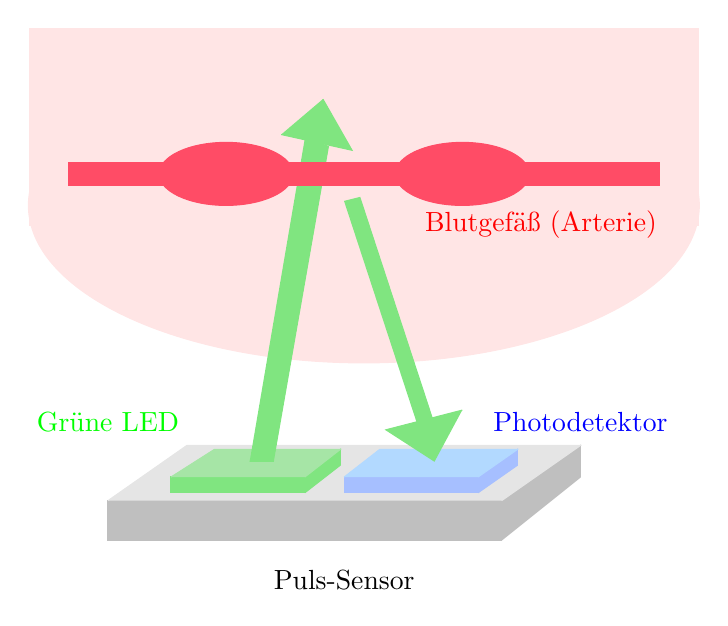
\begin{tikzpicture}
    \draw [fill=lightgray, draw=lightgray] (-2,0) rectangle (3,0.5);
    \draw [fill=lightgray, draw=lightgray] (3,0)--(4,0.8)--(4,1.2)--(3,0.5);
    \definecolor{verylightgray}{gray}{0.9};
    \draw [fill=verylightgray, draw=verylightgray] (-2,0.5)--(-1,1.2)--(4,1.2)--(3,0.5);
    
    \definecolor{lightgreen}{rgb}{0.5, 0.9, 0.5};
    \draw [fill=lightgreen, draw=lightgreen] (-1.2,0.6) rectangle (0.5,0.8);
    \draw [fill=lightgreen, draw=lightgreen] (0.5,0.8)--(0.95,1.15)--(0.95,0.95)--(0.5,0.6);
    
    \definecolor{hautfarbe}{rgb}{1, 0.9, 0.9};
    \draw [fill=hautfarbe, draw=hautfarbe] (-3,4) rectangle (5.5,6.5);
    \draw [fill=hautfarbe, draw=hautfarbe] (1.25,4.25) ellipse (4.26cm and 2cm);
    
    \definecolor{verylightgreen}{rgb}{0.65, 0.9, 0.65};
    \draw [fill=verylightgreen, draw=verylightgreen] (-1.2,0.8)--(-0.65,1.15)--(0.95,1.15)--(0.5,0.8);
    
    \definecolor{lightblue}{rgb}{0.65, 0.75, 1};
    \draw [fill=lightblue, draw=lightblue] (1,0.6) rectangle (2.7,0.8);
    \draw [fill=lightblue, draw=lightblue] (2.7,0.8)--(3.2,1.15)--(3.2,0.95)--(2.7,0.6);
    
    \definecolor{verylightblue}{rgb}{0.7, 0.85, 1};
    \draw [fill=verylightblue, draw=verylightblue] (1,0.8)--(1.45,1.15)--(3.2,1.15)--(2.7,0.8);
    
    \draw [fill=lightgreen, draw=lightgreen] (-0.2,1)--(0.1,1)--(0.8,5)--(0.5,5.1);
    \draw [fill=lightgreen, draw=lightgreen] (0.2,5.15)--(1.1,4.95)--(0.73,5.6);
    \draw [fill=lightgreen, draw=lightgreen] (1,4.3)--(1.2,4.35)--(2.2,1.3)--(2,1.25);
    \draw [fill=lightgreen, draw=lightgreen] (2.15,1)--(1.53,1.4)--(2.5,1.65);
    
    \definecolor{lightred}{rgb}{1, 0.3, 0.4};
    \draw [fill=lightred, draw=lightred] (0,4.5) rectangle (2,4.8);
    \draw [fill=lightred, draw=lightred](-0.5,4.65) ellipse (0.85cm and 0.4cm);
    \draw [fill=lightred, draw=lightred](2.5,4.65) ellipse (0.85cm and 0.4cm);
    \draw [fill=lightred, draw=lightred] (3,4.5) rectangle (5,4.8);
    \draw [fill=lightred, draw=lightred] (-0.5,4.5) rectangle (-2.5,4.8);
    
    \node[green] at (-2,1.5){Grüne LED};
    \node[blue] at (4,1.5){Photodetektor};
    \node at (1,-0.5){Puls-Sensor};
    \node[red] at (3.5,4){Blutgefäß (Arterie)};	
    
  \end{tikzpicture}

        \caption{Photoplethysmographie}
        \label{fig:Photoplethysmographie}	
    \end{figure}
    
    \begin{itemize}
        \item \textbf{Lichtquelle und Fotodetektor:} Der Sensor besteht aus \ac{led}s (meist grünes Licht) und einem Fotodetektor. Die LEDs senden Licht in die Haut.
        \item \textbf{Messung der Lichtreflexion:} Das Licht durchdringt die Haut und wird von den Blutgefäßen reflektiert. Der Fotodetektor misst die Menge des reflektierten Lichts.
        \item \textbf{Erkennung von Blutflussänderungen:} Bei jedem Herzschlag ändert sich die Menge des reflektierten Lichts aufgrund des veränderten Blutflusses in den Blutgefäßen. Diese Änderungen werden vom Fotodetektor erfasst.
        \item \textbf{Berechnung der Herzfrequenz:} Die Änderungen in der Lichtreflexion, die durch den Puls verursacht werden, werden zur Berechnung der Herzfrequenz genutzt.
    \end{itemize}
    
    \subsection{Der Photodetektor}
    
    \begin{itemize}[label={}]
        \item Der Photodetektor nutzt den Photoeffekt, auch als photoelektrischer Effekt bekannt. Der Photoeffekt ist ein physikalisches Phänomen, bei dem Elektronen aus einem Material (meist einem Metall) freigesetzt werden, wenn es mit Licht bestrahlt wird \cite{Traenkler:2014}.
        
        
        \begin{figure}[h]
            \centering
	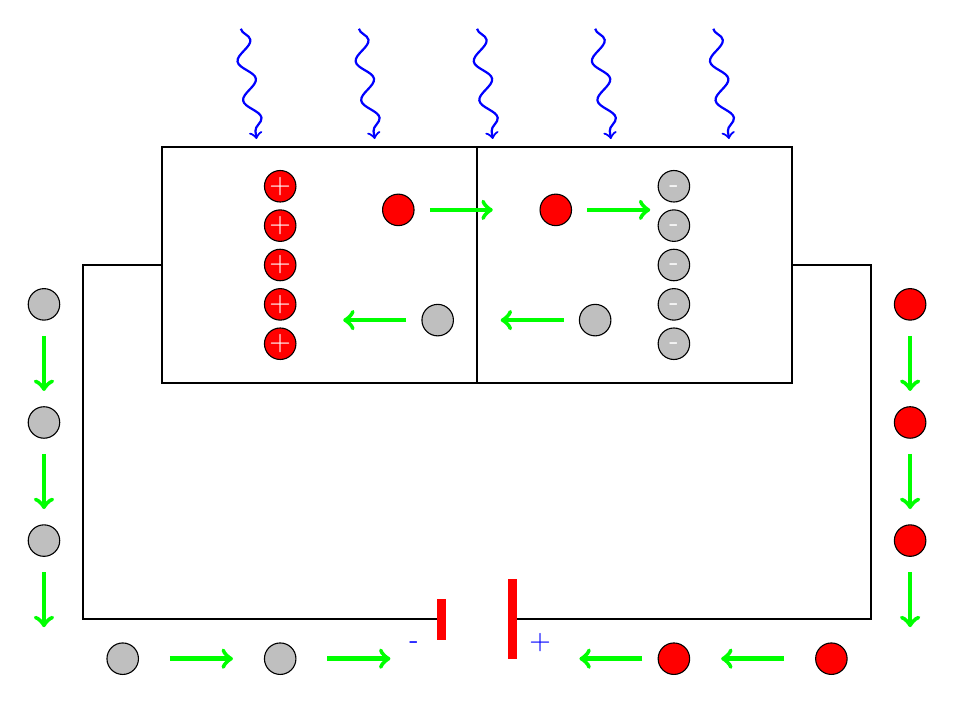
\begin{tikzpicture}
    \draw [thick] (0,0)rectangle(8,3);
    \draw (4,3)--(4,0);
    \draw [thick] (0,1.5)--(-1,1.5)--(-1,-3)--(3.5,-3);
    \draw [thick] (8,1.5)--(9,1.5)--(9,-3)--(4.5,-3);
    \draw [fill=red, draw=red] (3.5,-3.25) rectangle (3.6,-2.75);
    \draw [fill=red, draw=red] (4.5,-3.5) rectangle (4.4,-2.5);
    \node [thick,blue] at(3.2,-3.3){-};
    \node [thick,blue] at(4.8,-3.3){+};
    
    \draw[fill=lightgray] (6.5,0.5) circle (0.2cm);
    \draw[fill=lightgray] (6.5,1) circle (0.2cm);
    \draw[fill=lightgray] (6.5,1.5) circle (0.2cm);
    \draw[fill=lightgray] (6.5,2) circle (0.2cm);
    \draw[fill=lightgray] (6.5,2.5) circle (0.2cm);
    
    \draw[fill=red] (1.5,0.5) circle (0.2cm);
    \draw[fill=red] (1.5,1) circle (0.2cm);
    \draw[fill=red] (1.5,1.5) circle (0.2cm);
    \draw[fill=red] (1.5,2) circle (0.2cm);
    \draw[fill=red] (1.5,2.5) circle (0.2cm);
    
    \draw[fill=lightgray] (5.5,0.8) circle (0.2cm);
    \draw[fill=lightgray] (3.5,0.8) circle (0.2cm);
    
    \draw[->,ultra thick,green](5.1,0.8) -- (4.3,0.8);
    \draw[->,ultra thick,green](3.1,0.8) -- (2.3,0.8);
    
    \draw[fill=red] (3,2.2) circle (0.2cm);
    \draw[fill=red] (5,2.2) circle (0.2cm);
    
    \draw[->,ultra thick,green](3.4,2.2) -- (4.2,2.2);
    \draw[->,ultra thick,green](5.4,2.2) -- (6.2,2.2);
    
    \draw[fill=lightgray] (-1.5,-2) circle (0.2cm);
    \draw[fill=lightgray] (-1.5,1) circle (0.2cm);
    \draw[fill=lightgray] (-1.5,-0.5) circle (0.2cm);
    \draw[fill=lightgray] (-0.5,-3.5) circle (0.2cm);
    \draw[fill=lightgray] (1.5,-3.5) circle (0.2cm);
    
    \draw[->,ultra thick,green](-1.5,0.6) -- (-1.5,-0.1);
    \draw[->,ultra thick,green](-1.5,-0.9) -- (-1.5,-1.6);
    \draw[->,ultra thick,green](-1.5,-2.4) -- (-1.5,-3.1);
    \draw[->,ultra thick,green](0.1,-3.5) -- (0.9,-3.5);
    \draw[->,ultra thick,green](2.1,-3.5) -- (2.9,-3.5);
    
    \draw[fill=red] (9.5,-2) circle (0.2cm);
    \draw[fill=red] (9.5,1) circle (0.2cm);
    \draw[fill=red] (9.5,-0.5) circle (0.2cm);
    \draw[fill=red] (8.5,-3.5) circle (0.2cm);
    \draw[fill=red] (6.5,-3.5) circle (0.2cm);
    
    \draw[->,ultra thick,green](9.5,0.6) -- (9.5,-0.1);
    \draw[->,ultra thick,green](9.5,-0.9) -- (9.5,-1.6);
    \draw[->,ultra thick,green](9.5,-2.4) -- (9.5,-3.1);
    \draw[->,ultra thick,green](7.9,-3.5) -- (7.1,-3.5);
    \draw[->,ultra thick,green](6.1,-3.5) -- (5.3,-3.5);
    
    \draw[thick,blue,->, decorate, decoration={snake, amplitude=1mm, segment length=5mm}] (1,4.5) -- (1.2,3.1);
    \draw[thick,blue,->, decorate, decoration={snake, amplitude=1mm, segment length=5mm}] (2.5,4.5) -- (2.7,3.1);
    \draw[thick,blue,->, decorate, decoration={snake, amplitude=1mm, segment length=5mm}] (4,4.5) -- (4.2,3.1);
    \draw[thick,blue,->, decorate, decoration={snake, amplitude=1mm, segment length=5mm}] (5.5,4.5) -- (5.7,3.1);
    \draw[thick,blue,->, decorate, decoration={snake, amplitude=1mm, segment length=5mm}] (7,4.5) -- (7.2,3.1);
    
    \node [thick,white] at (6.5,0.5) {-};
    \node [thick,white] at (6.5,1) {-};
    \node [thick,white] at (6.5,1.5) {-};
    \node [thick,white] at (6.5,2) {-};
    \node [thick,white] at (6.5,2.5) {-};
    
    \node [thick,white] at (1.5,0.5) {+};
    \node [thick,white] at (1.5,1) {+};
    \node [thick,white] at (1.5,1.5) {+};
    \node [thick,white] at (1.5,2) {+};
    \node [thick,white] at (1.5,2.5) {+};
    
\end{tikzpicture}

            \caption{Der Photoeffekt}
            \label{fig:Photoeffekt}	
        \end{figure}
        
        \item \textbf{Ausgabe des Photodetektors}
        
        Der Photodetektor gibt eine Spannung aus, die über die Zeit gemessen wird. Diese Spannung variiert periodisch in Abhängigkeit von der Menge des reflektierten Lichts, das durch die Blutvolumenänderung aufgrund des Herzschlags beeinflusst wird.
        
        Die Spannungsänderung des Photodetektors ist also gleichzusetzen mit der Frequenz unseres Herzschlags \cite{Traenkler:2014}. 
    \end{itemize}
    
    
    \subsection{Spannungsdatenverarbeitung}
    
    Der Sensor ``GRV Heart Rate 3'' gibt analoge Spannungswerte im Bereich von 0 bis 3,3 Volt aus. Diese Spannungen werden vom Arduino über einen Analogeingang erfasst. Der Arduino nutzt seinen integrierten \ac{adc}, um diese analogen Spannungen in digitale Werte umzuwandeln.
    
    Der \ac{adc} des Arduino hat eine Auflösung von 10 Bit, was bedeutet, dass er Spannungen im Bereich von 0 bis 3,3 Volt in 1024 Schritte unterteilt. Somit wird eine Spannung von 0 Volt als digitaler Wert 0 und eine Spannung von 3,3 Volt als digitaler Wert 1023 dargestellt. Zwischen diesen beiden Extremen werden die Spannungswerte proportional in entsprechende digitale Werte umgewandelt.\cite{Parthier:2016}
    
    Diese Umwandlung ermöglicht es dem Arduino, die vom Sensor ausgegebenen analogen Spannungen als leicht verarbeitbare digitale Werte darzustellen. So kann der Arduino präzise Messungen durchführen und die Herzfrequenzdaten weiterverarbeiten. Im Code werden diese digitalen Werte dann verwendet, um die Herzfrequenz zu berechnen, indem die Anzahl der Spitzenwerte in den Spannungsdaten über eine bestimmte Zeitperiode gezählt und in Schläge pro Minute umgewandelt wird.
    
    \bigskip
    
    \begin{figure}[h]
        \hspace*{-2.5cm} % Verschiebt den Inhalt nach links
        \begin{adjustbox}{valign=t}
	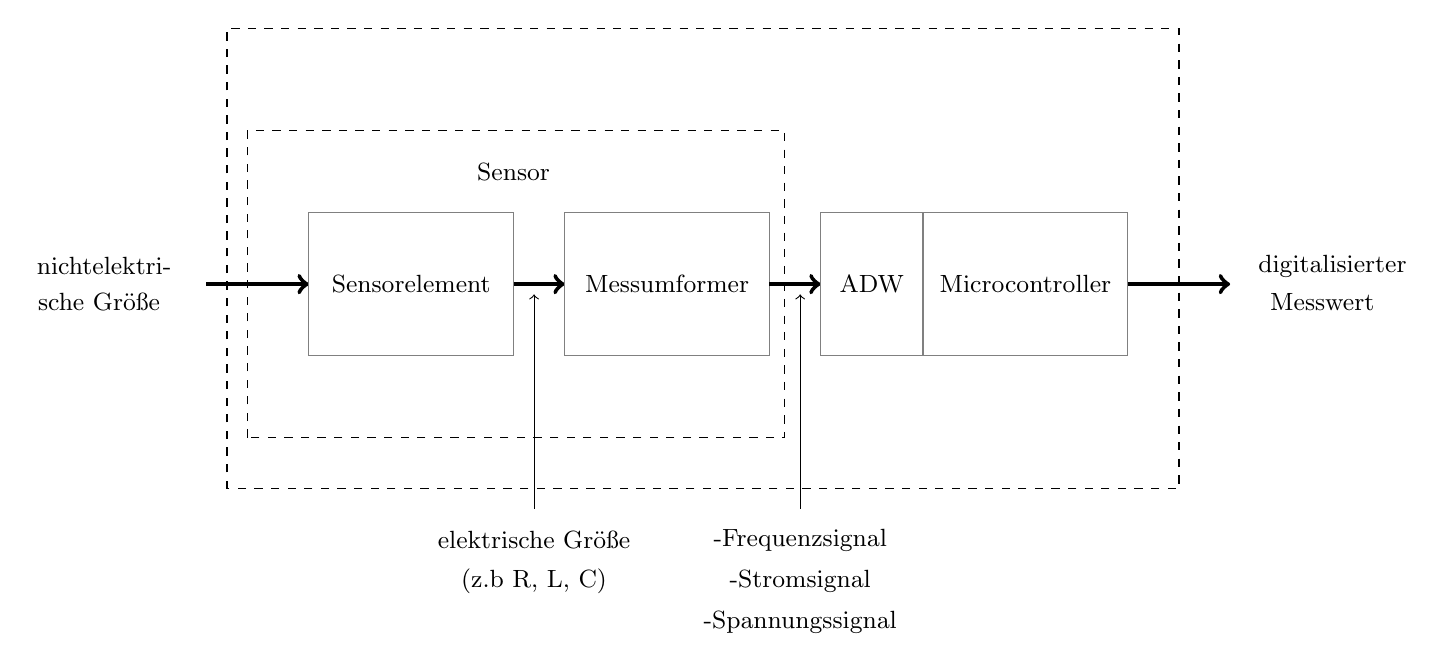
\begin{tikzpicture}[scale=1.3]
    \draw[->,ultra thick](0,0)--(1,0);
    \draw[gray] (1,-0.7) rectangle (3,0.7);
    \draw[->,ultra thick](3,0)--(3.5,0);
    \draw[gray] (3.5,-0.7) rectangle (5.5,0.7);
    \draw[->,ultra thick](5.5,0)--(6,0);
    \draw[gray] (6,-0.7) rectangle (9,0.7);
    \draw[gray] (7,-0.7)--(7,0.7);
    \draw[->,ultra thick](9,0)--(10,0);
    \draw[dashed](0.2,-2)rectangle(9.5,2.5);
    \draw[dashed](0.4,-1.5)rectangle(5.65,1.5);
    
    \draw[<-](3.2,-0.1)--(3.2,-2.2);
    \draw[<-](5.8,-0.1)--(5.8,-2.2);
    
    \node at (3.2,-2.5){\small elektrische Größe};
    \node at (3.2,-2.9){\small (z.b R, L, C)};
    
    \node at (5.8,-2.5){\small -Frequenzsignal};
    \node at (5.8,-2.9){\small -Stromsignal};
    \node at (5.8,-3.3){\small -Spannungssignal};
    
    \node at (3,1.1){\small Sensor};
    \node at (2,0){\small Sensorelement};
    \node at (4.5,0){\small Messumformer};
    \node at (6.5,0){\small ADW};
    \node at (8,0){\small Microcontroller};
    \node at (-1,0.175){\small nichtelektri-};
    \node at (-1.05,-0.175){\small sche Größe};
    
    \node at (11,0.175){\small digitalisierter};
    \node at (10.9,-0.175){\small Messwert};
\end{tikzpicture}

        \end{adjustbox}
        \centering
        \caption{Struktur eines Sensors}
        \label{fig}
    \end{figure}
    
    
    \subsection{Drift und Messungenauigkeiten}
    
    Drift kann eine wichtige Rolle beim Herzschlagsensor spielen. Drift bezieht sich auf die allmähliche Veränderung der Messwerte eines Sensors über die Zeit, die nicht auf tatsächliche Veränderungen des gemessenen Parameters zurückzuführen ist. Im Kontext eines Herzschlagsensors können verschiedene Arten von Drift auftreten.
    
    Ein Herzschlagsensor wandelt physiologische Messgrößen, wie die Blutflussänderungen, in elektrische Signale um, damit diese ausgewertet werden können. Allerdings kann es vorkommen, dass die Messwerte variieren, obwohl die Herzfrequenz konstant bleibt. Diese unerwünschte Veränderung der Messwerte wird als Drift bezeichnet \cite{Traenkler:2014}. Drift ist zeitabhängig und tritt aufgrund von Alterungsprozessen und inhärenten Ungenauigkeiten des Sensors auf. Im schlimmsten Fall kann Drift zu einem funktionalen Ausfall des Sensors führen.
    
    \begin{itemize}[label={}]
        \item  \textbf{Elektronische Drift} bezieht sich auf Veränderungen in der Elektronik des Sensors oder des Arduino-Boards selbst. Elektronische Komponenten können aufgrund von Temperaturänderungen, Alterung oder anderen Faktoren im Laufe der Zeit ihre Eigenschaften verändern, was zu einer Drift der Ausgangswerte führt.
        \item  \textbf{Optische Drift} tritt bei Herzschlagsensoren auf, die auf der Basis von Photoplethysmographie (PPG) arbeiten, indem sie die Lichtabsorption durch das Blut messen. Änderungen in den optischen Komponenten, wie LEDs oder Photodetektoren, können zu Drift führen, beispielsweise durch Verschmutzungen, Alterung der \ac{led}s oder Änderungen in der Durchlässigkeit des Gewebes.
        \item  \textbf{Mechanische Drift} kann durch mechanische Veränderungen oder Verschiebungen des Sensors auf der Haut verursacht werden. Eine schlechte oder sich ändernde Platzierung des Sensors kann die Genauigkeit der Messungen beeinträchtigen.
        \item  \textbf{Kalibrierungsdrift} tritt bei Herzschlagsensoren auf, die regelmäßige Kalibrierungen erfordern, um genaue Messungen zu gewährleisten. Ohne regelmäßige Kalibrierung kann der Sensor anfangen zu driften und ungenaue Messwerte liefern.
    \end{itemize}

    Um die Auswirkungen der Drift zu minimieren, können mehrere Maßnahmen ergriffen werden:
    
    \begin{itemize}[label={}]
        \item \textbf{Regelmäßige Kalibrierung}: Falls der Sensor eine Kalibrierung benötigt, sollte diese regelmäßig durchgeführt werden, um sicherzustellen, dass die Messungen genau bleiben.
        \item \textbf{Kontinuierliche Überwachung}: Durch kontinuierliche Überwachung der Ausgangswerte und Vergleich mit bekannten Referenzwerten (z.B. Vergleich mit einem klinisch validierten Gerät) kann Drift erkannt und korrigiert werden.
        \item \textbf{Platzierung des Sensors}: Eine konsistente und stabile Platzierung des Sensors am Körper kann mechanische Drift minimieren. Idealerweise sollte der Sensor an einer Stelle befestigt werden, die wenig Bewegung ausgesetzt ist, wie das Ohrläppchen.
        \item \textbf{Umgebungskontrolle}: Durch Kontrolle der Umgebungstemperatur und -bedingungen kann elektronische Drift reduziert werden.
    \end{itemize}
    
    Durch die Berücksichtigung dieser Maßnahmen kann die Genauigkeit und Zuverlässigkeit der Herzfrequenzmessungen mit dem Herzschlagsensor verbessert werden \cite{Traenkler:2014}.
    
}


\section{Herzschlagsensor mit Grove-Schnittstelle und Ohr-Clip}

Das Kit ``GRV HEART RATE3 Ear Clip'' besteht aus einem Ohrclip und einem Empfängermodul und ist speziell für die Messung der Herzfrequenz bei Patienten und Sportlern konzipiert. Die gemessenen Daten können entweder in Echtzeit auf einem Monitor über einen seriellen Port angezeigt oder für spätere Analysen gespeichert werden. Das System zeichnet sich durch seine hohe Empfindlichkeit, geringen Stromverbrauch und hohe Mobilität aus. \Mynote{werbung}

\begin{figure}[h]
    \begin{center}
        \includegraphics[width=12cm]{HeartRate/HeartRateSensor}
        \caption{Grove-Herzschlag-Sensor mit Ohr-Clip\cite{Seeed:2015}}
        \label{fig:Herzschlagsensor}
    \end{center}
\end{figure}


\subsubsection{Technische Merkmale}

\begin{description}
    \item{Niedriger Stromverbrauch}
    \item{Große Bandbreite beim Eingangsstrom:} 3 - 5 V (Gleichstrom)
    \item{Bequeme Verwendung}
    \item{Hohe Empfindlichkeit}
\end{description}

\subsubsection{Technische Daten}

\begin{description}
    \item{Anschlusstyp:} Steckverbinder JST-VH
    \item{Anschlusssystem:} Grove-Schnittstelle
\end{description} 
\cite{Seeed:2015}



\subsection{Testen des Herzschlagsensors}

Um den Herzschlagsensor zu testen, wird ein einfaches Programm verwendet, mit dem man die Peaks erkennt. Der Herzfrequenzsensor wird an den analogen Pin A0 angeschlossen und der gemessene Wert alle 500 Millisekunden über die serielle Schnittstelle an den Computer gesendet wird. Die serielle Ausgabe über den Plotter wird in einem Diagramm dargestellt, das periodische Herzfrequenzsignale zeigt. Die Werte schwanken zwischen 0 und 1023, was auf die erkannten Peaks des Herzschlagsensors hinweist. Dies bestätigt, dass der Sensor ordnungsgemäß funktioniert und die Herzfrequenzdaten erfolgreich erfasst und visualisiert werden.


\begin{figure}[h]
    \begin{center}
        \includegraphics[width=10cm]{HeartRate/HeartRateTestDiagramm}
        \caption{Herzschlag Diagramm (Test)}
        \label{fig:HerzschlagDiagramm}	
    \end{center}
\end{figure}

\begin{code}[h]
    \pythonexternal[language=c++]{../../Code/Arduino/HeartRate/TestHeartRateSensor.ino}
    \caption{Testprogramm Herzschlagsensor} 
    \label{Code:Arduino:HeartRateSensor}
\end{code}


\subsection{Programmcode und Dokumentation}
% Code block with proper placement

\begin{code}[h]
    \
    external[language=c++, linerange={1-11}, firstnumber=1]{../../Code/Arduino/HeartRate/HeartRate.ino}
\end{code}

Zu Beginn des Codes werden die notwendigen Bibliotheken eingebunden. \FILE{Arduino.h} wird für die allgemeine Programmierung auf der Arduino-Plattform benötigt. \FILE{U8g2lib} ist eine Bibliothek für die Ansteuerung von \ac{oled}-Displays, \FILE{SPI.h} und \FILE{SD.h} ermöglichen die Kommunikation mit der SD-Karte. Zusätzlich wird durch bedingte Kompilierung (\PYTHON{\#ifdef U8X8\_HAVE\_HW\_SPI} und \PYTHON{\#ifdef U8X8\_HAVE\_HW\_I2C}) geprüft, ob die Hardware-Schnittstellen \ac{spi} und \ac{i2c} verfügbar sind und die entsprechenden Bibliotheken werden eingebunden, falls sie vorhanden sind. Diese bedingten Einbindungen sind wichtig, um sicherzustellen, dass die richtigen Bibliotheken nur dann geladen werden, wenn die entsprechende Hardware tatsächlich vorhanden ist.

\begin{code}[h]
    \pythonexternal[language=c++, linerange={12-18}, firstnumber=12]{../../Code/Arduino/HeartRate/HeartRate.ino}
\end{code}

In diesen Zeilen wird das Display initialisiert. \PYTHON{U8G2\_SH1106\_128X64\_NONAME\_F\_HW\_I2C u8g2(U8G2\_R0, U8X8\_PIN\_NONE, A5, A4);} erstellt ein Objekt \PYTHON{u8g2} für das OLED-Display, das über \ac{i2c} kommuniziert. Die Pins für den Herzfrequenzsensor (\PYTHON{heartRatePin}), die Batterie (\PYTHON{batteryPin}) und das \ac{sd}-Karten Modul(\PYTHON{chipSelect}) werden ebenfalls definiert.



\begin{code}[h]
    \pythonexternal[language=c++, linerange={19-31}, firstnumber=19]{../../Code/Arduino/HeartRate/HeartRate.ino}
\end{code}

Hier werden verschiedene Variablen definiert, die zur Speicherung und Verarbeitung der Herzfrequenzdaten verwendet werden. \PYTHON{heartRateValue} und \PYTHON{lastHeartRateValue} speichern die aktuellen und vorherigen Herzfrequenzwerte. \PYTHON{lastPeakTime} und \PYTHON{lastHeartbeatTime} speichern die Zeitpunkte der letzten Peaks und Herzschläge. \PYTHON{peakDetected} ist ein boolescher Wert, der angibt, ob ein Peak erkannt wurde. \PYTHON{threshold} ist der Schwellenwert zur Erkennung eines Herzschlags. \PYTHON{heartRate}, \PYTHON{heartRateArray}, \PYTHON{heartRateIndex}, \PYTHON{heartRateSum} und \PYTHON{previousHeartRate} werden zur Berechnung und Speicherung der Herzfrequenz verwendet. \PYTHON{errorTimeout} und \PYTHON{errorState} dienen zur Fehlerüberwachung.


\begin{code}[h]
    \pythonexternal[language=c++, linerange={32-41}, firstnumber=31]{../../Code/Arduino/HeartRate/HeartRate.ino}
\end{code}

\noindent Dieser Abschnitt definiert weitere Variablen zur Steuerung des Anzeigemodus und zur Speicherung der Graphdaten. \PYTHON{lastSwitchTime} und \PYTHON{switchInterval} werden zur Verwaltung des Anzeigemodus verwendet, \PYTHON{showGraph} gibt an, ob der Graph angezeigt wird. \PYTHON{graphData} speichert die Herzfrequenzdaten für die Darstellung im Graphen. \PYTHON{sdCardFull} überprüft, ob die \ac{sd}-Karte voll ist, \PYTHON{startTime} speichert die Startzeit des Arduino und \PYTHON{initialMeasurement} ist ein boolescher Wert, der anzeigt, ob sich das Programm in der initialen Messperiode befindet.



\begin{code}[h]
    \pythonexternal[language=c++, linerange={42-76}, firstnumber=42]{../../Code/Arduino/HeartRate/HeartRate.ino}
\end{code}

Die Funktion  \PYTHON{setup()} initialisiert die serielle Kommunikation mit einer Baudrate von 9600, setzt die Pins für den Herzfrequenzsensor und die Batterie als Eingänge und initialisiert das Display. Zudem wird die \ac{sd}-Karte initialisiert und,  falls die Initialisierung fehlschlägt, wird dies über die serielle Schnittstelle ausgegeben. Anschließend wird ein Startbildschirm auf dem Display angezeigt und die Startzeit gespeichert.

\begin{code}[h]
    \pythonexternal[language=c++, linerange={77-135}, firstnumber=77]{../../Code/Arduino/HeartRate/HeartRate.ino}
\end{code}


\begin{code}[h]
    \pythonexternal[language=c++, linerange={135-173}, firstnumber=135]{../../Code/Arduino/HeartRate/HeartRate.ino}
\end{code}


In der Funktion \PYTHON{loop()} wird die Hauptlogik des Programms ausgeführt. Zunächst wird eine initiale Wartezeit von 5 Sekunden implementiert, um sicherzustellen, dass das System stabil ist, bevor Messungen durchgeführt werden. Falls die \ac{sd}-Karte voll ist, wird die Schleife beendet. Es werden die Herzfrequenz- und Batteriespannungswerte gelesen und die Spannung auf dem seriellen Monitor ausgegeben. Wird ein Herzfrequenzpeak erkannt, wird die Zeit seit dem letzten Peak berechnet und die Herzfrequenz daraus abgeleitet. Diese Werte werden dann auf dem Display angezeigt und auf der \ac{sd}-Karte gespeichert. Zusätzlich werden Graphdaten aktualisiert und Fehlerzustände überwacht. Die Anzeige wechselt alle 10 Sekunden zwischen Text- und Graphmodus, sofern kein Fehlerzustand vorliegt.

\begin{code}[h]
    \pythonexternal[language=c++, linerange={173-183}, firstnumber=173]{../../Code/Arduino/HeartRate/HeartRate.ino}
\end{code}

Die Funktion \PYTHON{drawBattery(float voltage)} zeichnet die Batteriestandsanzeige auf das Display, basierend auf der gemessenen Spannung. Die Spannung wird in einen Wert zwischen 0 und 4 umgewandelt, um den Ladezustand der Batterie darzustellen.


\begin{code}[h]
    \pythonexternal[language=c++, linerange={184-193}, firstnumber=184]{../../Code/Arduino/HeartRate/HeartRate.ino}
\end{code}


In der Funktion \PYTHON{updateGraph(int heartRate)} werden die Herzfrequenzdaten aktualisiert. Die alten Daten werden nach links verschoben und die neue Herzfrequenz wird am Ende des Arrays gespeichert. Falls die Herzfrequenz unter 40 Schläge pro Minute fällt, wird der Wert auf 0 gesetzt. Diese Funktion stellt sicher, dass der Graph immer aktuelle Daten anzeigt und alte Daten kontinuierlich durch neue ersetzt werden.

\begin{code}[h]
    \pythonexternal[language=c++, linerange={195-217}, firstnumber=195]{../../Code/Arduino/HeartRate/HeartRate.ino}
\end{code}

Die Funktion \PYTHON{drawGraph()} zeichnet den Verlauf der Herzfrequenz als Graph auf das Display. Dazu werden die Herzfrequenzdaten über die Zeit aufgetragen und als Liniengraph dargestellt. Die Achsen und Beschriftungen werden ebenfalls gezeichnet. 


\begin{code}[h]
    \pythonexternal[language=c++, linerange={218-237}, firstnumber=218]{../../Code/Arduino/HeartRate/HeartRate.ino}
\end{code}

Die Funktion \PYTHON{saveToSD(int heartRate)} speichert die Herzfrequenzdaten auf der \ac{sd}-Karte. Wenn ein Fehler beim Öffnen der Datei auftritt, wird dies auf dem Display angezeigt und das Programm erkennt, dass die \ac{sd}-Karte voll sein könnte. Dies stellt sicher, dass alle Daten sicher gespeichert werden und der Benutzer informiert wird, falls ein Speicherproblem auftritt.



\section{Kalibrierung}

Wir haben den Herzschlagsensor kalibriert, indem wir die von ihm ausgegebenen Werte gleichzeitig mit den Herzschlagwerten einer Person auf einer Apple Watch abgeglichen und verglichen haben. Erstaunlicherweise stimmten die Werte genau überein, was die Genauigkeit des Sensors bestätigte.



%%%
%
% $Autor: Wings $
% $Datum: 2021-05-14 $
% $Pfad: GitLab/MLEdgeComputer $
% $Dateiname: Grove
% $Version: 4620 $
%
% !TeX spellcheck = de_DE/GB
% !TeX program = pdflatex
% !BIB program = biber/bibtex
% !TeX encoding = utf8
%
%%%

\chapter{Grove}

Grove, ein Produkt von Seeed Studio, ist eine Hardware-Schnittstelle für Technikinteressierte. Es vereinfacht die Kommunikation zwischen Mikrocontrollern und Sensoren und reduziert das Löten. Diese Schnittstelle wurde im Jahr 2010 von Seeed Studio entwickelt, um die Zusammenarbeit zwischen verschiedenen Technologien zu vereinfachen und die Entwicklung neuer Projekte zu erleichtern.\cite{Seeed:2012,Seeed:2013}

Mit der Verfügbarkeit eines Steckverbinder-Typs bietet diese Schnittstelle eine Vielzahl von Möglichkeiten für die Integration von Sensoren, Aktuatoren und Mikrocontrollern. Diese einfachen Kommunikationsverbindungen ermöglichen es den Nutzern, ihre Projekte ohne großen Zeitaufwand zu realisieren und zu testen. \cite{Seeed:2016} Mit jedem neuen Sensor, der mit der Grove-Familie auf dem Markt erscheint, wird die Flexibilität und kreative Möglichkeit für die Entwicklung von Projekten weiter gesteigert. 




Die meisten Mikrocontroller verfügen nicht unmittelbar über die Grove-Schnittstelle. Damit Komponenten, die die Grove-Schnittstelle haben, werden häufiger Shields eingesetzt, die diese dann zur Verfügung stellt. Zum Beispiel verfügt  der Arduino Nano 33 BLE Sense Lite über keine Grove-Anschlüsse. Das Tiny Machine Learning Shield ermöglicht die Verwendung von Grove-Komponenten für den Arduino Nano 33 BLE Sense, indem es als Schnittstelle zwischen dem Mikrocontroller und den Grove-Modulen fungiert. Der Arduino Nano 33 BLE Sense wird direkt auf das Shield gesteckt, welches über standardisierte Grove-Anschlüsse verfügt. Auf der Abbildung~\ref{GroveMikrocontrollerShield} ist dargestellt, wie der Mikrocontroller Arduino Nano 33 BLE Sense mit dem Shield verbunden ist.

    \begin{center}
        \includegraphics[width=\textwidth]{Grove/Shield.jpg}
        \captionof{figure}{Mikrocontroller gesteckt auf dem Shield}
        \label{GroveMikrocontrollerShield}
    \end{center}


\section{Grove-Universal-Kabel}

Üblicherweise werden Sensoren und Mikrocontroller über ein Grove-Universal-Kabel verbunden. In der Abbildung~\ref{GroveUniversalCable}, vom Hersteller \textit{seeed studio} ermöglicht die Verbindung mit allen Modulen des Grove-Systems. Für ein Grove-System wird somit nur eine Kabelart benötigt. Die Schnittstellen des Kabels sind beidseitig \ac{jst}-VH-Stecker. In der Abbildung~\ref{GroveUniversalCable} beträgt beispielsweise die Kabellänge  50 mm \cite{Seeed:2016}. 

\begin{figure}[h]
    \begin{center}
        \includegraphics[width=3in]{Grove/UniversalCable.jpg}
        \caption{Grove-Universal-Kabel\cite{Reichelt:2024b}}
        \label{GroveUniversalCable}
    \end{center}
\end{figure}

\section{Verbindung Grove-Schnittstelle zu 4-Pin-Lösungen}

Da nicht alle Sensoren und Mikrocontroller über eine Grove-Schnittstelle verfügen, existieren Kabel, die einseitig die Grove-Schnittstelle haben. In der Abbildung~\ref{GroveJumperZuGrove4PinKabel} ist das Kabel dargestellt, das auf einer Seite die Grove-Schnittstelle zur Verfügng stellt und auf der anderen Seite 4 Pins. In diesem Beispiel hat das Kabel  eine Länge von 30 cm \cite{Reichelt:2024g}.

    \begin{center}
        \includegraphics[width=3in]{Grove/Grove2Pin}
        \captionof{figure}{Grove Jumper zu Grove 4 Pin-Kabel\cite{Reichelt:2024g}}
        \label{GroveJumperZuGrove4PinKabel}
    \end{center}


\section{Pinbelegung}

Die Pinbelegung ist von seeed studio standardisiert. In der Tabelle~\ref{PinBelegungGrove} ist die Belegung erläutert. \cite{Seeed:2016}

    \begin{center}
        \captionof{table}{Pinbelegung der Grove-Schnittstelle}
        \begin{tabular}{l|l|l}
            Farbe & Pin & Funktion \\ \hline
            Gelb    & 1   & frei belegbar, D0 oder A0 \\
            Weiß    & 2   & frei belegbar, D1 oder A1 \\
            Rot     & 3   &   VCC,  3,3V oder 5V \\
            Schwarz & 4   & \acs{gnd} \\
            
        \end{tabular}
        \label{PinBelegungGrove}
    \end{center}

Grove stellt über Pin 3 und 4 die Stromversorgung sicher. Der gelbe und der weiße Pin ist in Abhängigkeit vom Sensor belegt. Falls der Sensor nur einen Pin benötigt, so wird Pin 1 verwendet.  Als Schnittstelle zum Mikrocontroller muss die Belegung für jede Anwendung definiert werden. 

Für Protokolle, wie zum Beispiel I\textsuperscript{2}C und \ac{spi}, sind die Belegung eindeutig festgelegt. Die Tabelle\ref{GrovePinBelegungI2C} listet die Pinbelegung der Grove-Schnittstelle für I\textsuperscript{2}C-Grove-Stecker auf.

\begin{center}
    \captionof{table}{Pinbelegung der Grove-Schnittstelle für I\textsuperscript{2}C-Grove-Stecker}
    \begin{tabular}{l|l|l}
        Farbe & Pin & Funktion \\ \hline
        Gelb    & 1   & frei belegbar, zum Beispiel SCL auf I\textsuperscript{2}C-Grove-Steckern \\
        Weiß    & 2   & frei belegbar, zum Beispiel SDA auf I\textsuperscript{2}C-Grove-Steckern \\
        Rot     & 3   &   VCC,  3,3V oder 5V \\
        Schwarz & 4   & \acs{gnd} \\
        
    \end{tabular}
    \label{GrovePinBelegungI2C}
\end{center}

Die Tabelle~\ref{GrovePinBelegungUART} enthält die Pinbelegung für die serielle Schnittstelle UART.

    \begin{center}
    \captionof{table}{Pinbelegung der Grove-Schnittstelle für UART}
    \begin{tabular}{l|l|l}
        Farbe & Pin & Funktion \\ \hline
        Gelb    & 1   & RX\\
        Weiß    & 2   & TX \\
        Rot     & 3   & VCC,  3,3V oder 5V \\
        Schwarz & 4   & \acs{gnd} \\
        
    \end{tabular}
    \label{GrovePinBelegungUART}
\end{center}




%%%
%
% $Autor: Wings $
% $Datum: 2021-05-14 $
% $Pfad: GitLab/MLEdgeComputer $
% $Dateiname: SensorHCSR04
% $Version: 4620 $
%
% !TeX spellcheck = de_DE/GB
% !TeX program = pdflatex
% !BIB program = biber/bibtex
% !TeX encoding = utf8
%
%%%

\chapter{Ultraschallsensor HC-SR04}


Introduction
\Mynote{cite books, applications, board}

\section{Domänenwissen}
Im folgenden Abschnitt wird der namensgebende Sensor für diese Arbeit näher betrachtet. Dazu zählen seine physikalischen Grundlagen, seine Funktionsweise und Anwendungsbeispiele aus Industrie und Medizin.

\section{Grundlagen zur Verwendung eines Ultraschallsensors}

\subsection{Grundlagen Schall}

Als Schall bezeichnet man die Ausbreitung von lokalen Druckschwankungen in einem elastischen Medium. Die Schallwelle breitet sich dabei longitudinal aus, die Auslenkung der Moleküle erfolgt also in Ausbreitungsrichtung \cite{Tippler:2024}.
Die Einteilung der Schallbereiche erfolgt auf Grundlage der Frequenz:

\begin{itemize}
    \item \textit{Infraschall:} bis 16 Hz,
    \item \textit{Hörbarer Schall:} von 16 Hz bis 20 kHz,
    \item \textit{Ultraschall:} von 20 kHz bis 1 GHz,
    \item \textit{Hyperschall:} über 1 GHz \cite{Hering:2023}.
\end{itemize}

\Mynote{Grafik fehlt}


\subsection{Schallgeschwindigkeit und Wellenlänge}\label{AbschnittVschall}

Die Geschwindigkeit, mit der sich Schall in Luft ausbreitet, ist von der Lufttemperatur $T$ und der Luftfeuchtigkeit $\varphi$ abhängig. Da die Luftfeuchtigkeit einen erheblich geringeren Einfluss auf den Wert hat 

\begin{equation}
    \Delta v_{Schall,\varphi}\approx1,2\:\dfrac{\text{m}}{\text{s}}; \:0<\varphi<1, \:T_{C}=20 \:\text{\textcelsius},
    \label{Vphi}
\end{equation}

\cite{Hering:2023} lässt sich die Schallgeschwindigkeit mit ausreichender Genauigkeit mit der Formel \ref{Vschall}

\begin{equation}
    v_{Schall}=\sqrt{\kappa R T}
    \label{Vschall}
\end{equation} 

und der Annahme $\varphi=0$ berechnen \cite{Tippler:2024}. 
Dabei ist $\kappa = 1{,}4$ der Adiabatenexponent von Luft, $R=287$ \(\dfrac{\text{J}}{\text{kg K}}\) die spezifische Gaskonstante von Luft und $T$ die absolute Temperatur in Kelvin \cite{Tippler:2024,Willems:2022}.
Für eine angenommene Temperatur von $T_{C} = 20\:\text{\textcelsius}$ ergibt sich damit eine Geschwindigkeit von $v_{Schall}=343,2\:\dfrac{\text{m}}{\text{s}}$.
In Abb. \ref{schallfunktion} ist die Schallgeschwindigkeit in Luft im Temperaturbereich von $T_{C} = -10 \:\text{\textcelsius \:bis} \:60 \:\text{\textcelsius}$ dargestellt.

\begin{figure}[h]
    \begin{center}
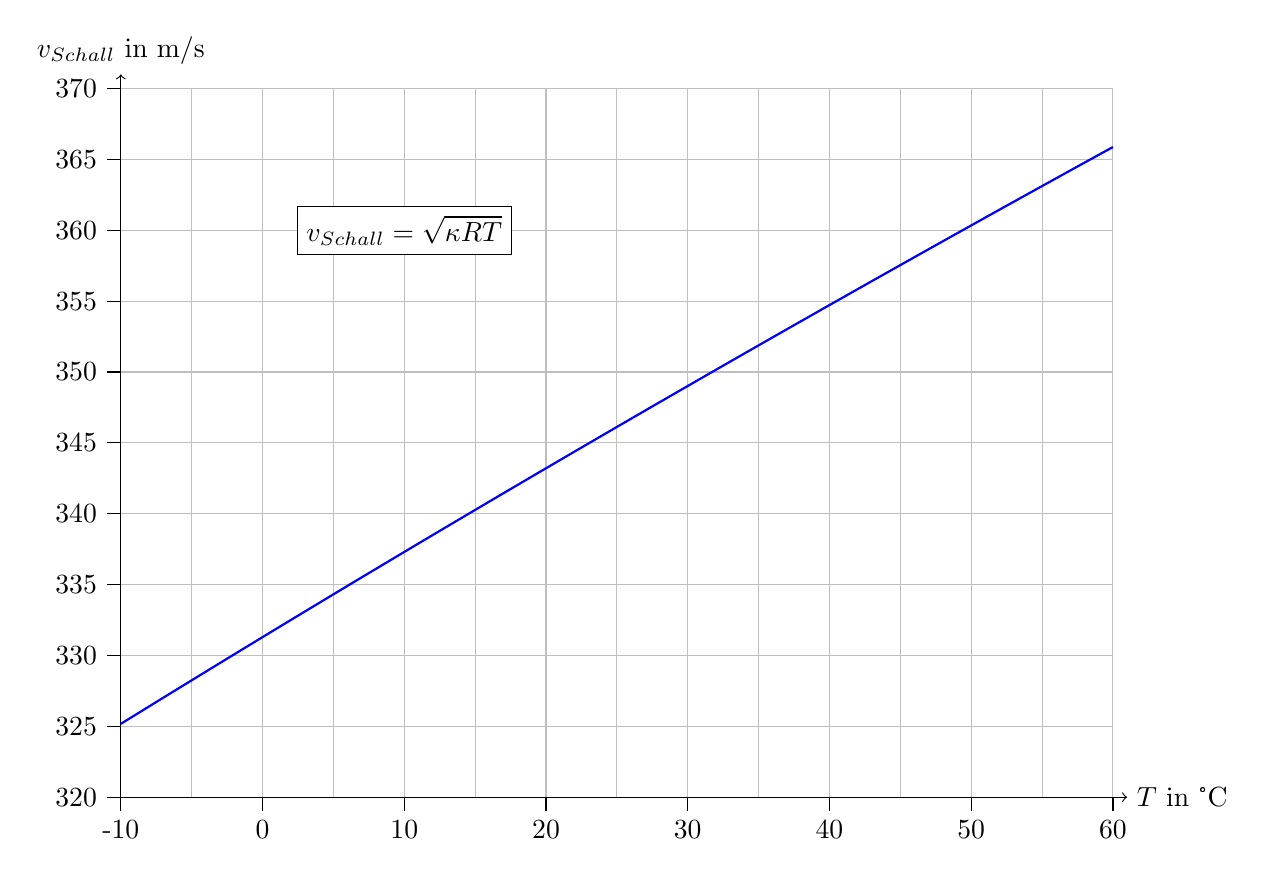
\begin{tikzpicture}
    \begin{scope}[scale=.9]
        %Gitter im Hintergrund
        \draw[lightgray] (-2,4) grid (12,14); 
        
        %Achsen
        \draw[thin, ->] (-2,4) -- (12.2,4) node[right] {$T$ in °C}; %x-Achse
        \draw[thin, ->] (-2,4) -- (-2,14.2) node[above] {$v_{Schall}$ in m/s}; %y-Achse
        %Beschriftung
        \foreach[count=\x] \a in {-10, 0, 10, 20, 30, 40, 50, 60} {
            \draw[thin] (2*\x-4,4) -- (2*\x-4,3.8) node [below] {\a};
        }%x-Achse
        \foreach[count=\x] \a in {320, 325, ..., 370} {
            \draw[thin] (-2,\x+3) -- (-2.2,\x+3) node [left] {\a};
        }%y-Achse
        
        %Funktion
        \draw[scale=2, thick, domain=26.316:33.316, variable=\T, blue] plot ({\T-27.316}, {sqrt(\T*40.18)-30});
        \node at(2,12) [rectangle,fill=white, draw] {$v_{Schall}=\sqrt{\kappa R T}$};
        
        %Vergleichsfunktion
        %\draw[gray] plot coordinates {(-2,5) (12,13.2)};
    \end{scope}
\end{tikzpicture}        \caption{Ausbreitungsgeschwindigkeit von Schall in Luft}
        \label{schallfunktion}
    \end{center}
\end{figure}

Über den Formelzusammenhang \ref{Wellenlaenge}

\begin{equation}
    v_{Schall}=\lambda f
    \label{Wellenlaenge}
\end{equation}

lässt sich bei gegebener Frequenz $f$ und mit der berechneten Schallgeschwindigkeit $v_{Schall}$ die Wellenlänge des Schalls berechnen \cite{Willems:2022}. Diese beträgt bei einer angenommenen Frequenz von $f=40 \:\text{kHz}$ und der in Abschnitt \ref{AbschnittVschall} berechneten Schallgeschwindigkeit $\lambda=8{,}58*10^{-3} \:\text{m}$.

\subsection{Absorption und Reflexion}

Absorption beschreibt die Abnahme der Intensität $I$ einer Schallwelle, während sie Weg durch das sie leitenden Medium zurücklegt. Sie ist vom Quadrat der Frequenz $f$ des Schalls und den Absorptionseigenschaften $a$ des Ausbreitungsmediums abhängig und lässt sich über die Formel \ref{Absorption}

\begin{equation}
    I(x)=I_0\times\exp(-\alpha x); \:\alpha=af^2
    \label{Absorption}
\end{equation}

berechnen \cite{Hering:2023,Hering:2021b}.
In Abbildung~\ref{DiagrammIntensitaet} ist die Abhängigkeit des Verhältnisses der Intensität $I$ zu $I_0$ von der Frequenz dargestellt. Die Wegstrecke von einem Meter und die Umgebungsbedingungen sind entsprechend konstant.

Für eine Frequenz von $f=40 \:\text{kHz}$ ergibt sich ein Verhältnis von 0,95.

\begin{figure}[h]
    \begin{center}
%Diagramm Intensität
%Abstandssensor\Entwicklerdokumentation\tikz
%tikz-Diagramm für die Abhängigkeit der Intensität von der Frequenz (qualitativ)
%Bestandteil der Entwicklerdokumentation "Abstandssensor" (Automatisierungstechnik SS24)

\begin{tikzpicture}
    \begin{scope}[scale=.85]	
        %Achsen
        \draw[thin, ->] (0,0) -- (10.2,0) node[right] {$f$ in KHz}; %x-Achse
        \draw[thin, ->] (0,0) -- (0,8.2) node[above] {$I/I_0$}; %y-Achse
        %Beschriftung
        \foreach[count=\x] \a in {0, 20, ..., 200} {
            \draw[thin] (\x-1,0) -- (\x-1,-0.2) node [below] {\a};
        }%x-Achse
        \foreach[count=\x] \a in {0.0001, 0.0010, 0.0100, 0.1000, 1.0000} {
            \draw[thin] (0,\x*2-2) -- (-0.2,\x*2-2) node [left] {\a};
        }%y-Achse
        
        %Funktion, qualitativ!
        \draw[thick, domain=0:10, variable=\x, blue] plot ({\x}, {-0.0741*\x^2+8});
    \end{scope}
\end{tikzpicture}
        \caption{Abnahme der Schallintensität in Abhängigkeit der Frequenz bei einem Meter, nach \cite{Hering:2023}}
        \label{DiagrammIntensitaet}
    \end{center}
\end{figure}

Trifft die Schallwelle auf die Grenzschicht zweier Medien mit verschiedenen Schallkennimpedanzen $Z_n$, wird sie zum Teil reflektiert und zum anderen Teil transmittiert. Der Reflexionsgrad ist bei großen Differenzen zwischen den Impedanzen $\left(Z_1 \ll Z_2 \:\text{oder} \:Z_1 \gg Z_2\right)$ der Medien besonders hoch. Sind die Impedanzen hingegen ähnlich $\left(Z_1 \approx Z_2\right)$ ist der Absorptionsgrad sehr hoch \cite{Hering:2021b}. 
Da viele Flüssigkeiten und feste Stoffe eine um den Faktor $10^4 \:\text{bis} \:10^5$ höhere Impedanz im Vergleich zu Luft vorweisen, ist der Reflexionsgrad in diesen Fällen $\gg 99\%$ \cite{Hering:2021b,Hering:2023}.

\subsection{Weg- und Abstandsmessung mit Ultraschall}

Um eine Entfernung oder einen Abstand eines Objekts zu dem Sensor zu ermitteln, wird der Sensor im sog. \textit{Tastbetrieb mit Echo-Laufzeit-Messung}, wie in Abb. \ref{TastbetriebELM} zu sehen, verwendet. Dabei sendet der Sensor zunächst ein Schallpuls in Richtung des zu messenden Objekts aus (Lautsprecher), welche zum Teil von diesem reflektiert wird und somit zurück zum Sensor gelangt (Echo). Dieses Echo kann der Sensor detektieren (Mikrofon) und über die gemessene Laufzeit des Echos sowie die Schallgeschwindigkeit im dem den Sensor umgebenden Medium die Distanz berechnen \cite{Hering:2023}.

\begin{figure}[h]
    \begin{center}
%Funktionsweise
%Abstandssensor\Entwicklerdokumentation\tikz
%tikz-Diagramm zur Funktionsweise eines Ultraschallsensors (qualitativ)
%Bestandteil der Entwicklerdokumentation "Abstandssensor" (Automatisierungstechnik SS24)

\begin{tikzpicture}
    %Achsen
    \draw[thin, ->] (0,0) -- (10.2,0) node[right] {$t$}; %x-Achse
    \draw[thin, ->] (0,0) -- (0,4.2) node[above] {$U$}; %y-Achse
    
    %Funktion, qualitativ!
    \draw[thick, blue] plot [smooth] coordinates{(1,0) (2,3) (4,3.5) (4.5,1) (5,0.1) (6,0)};
    \draw[thick, blue] plot [smooth] coordinates{(8,0) (8.3,0.1) (9,0.8) (9.7,0.1) (10,0)};
    
    %Beschriftung
    \node at (1,0) [anchor=south east] {$t_0$};
    \node at (8,0) [anchor=south east] {$t_1$};
    \draw[dotted] (4.5,1) -- (5,2) node[anchor=south west]{Sendeimpuls}; 
    \draw[dotted] (9,0.8) -- (9.5,2) node[anchor=south]{Echo}; 
    \draw (1,0) -- (1,-2.2);
    \draw (8,0) -- (8,-2.2);
    \draw[<->] (1,-2) -- (4.5,-2) node[anchor=south]{Echolaufzeit} -- (8,-2);
    \draw (4,0) -- (4,-1.2); 
    \draw (6,0) -- (6,-1.2); 
    \draw[<->] (1,-1) -- (2.5,-1) node[anchor=south]{$\delta t$} -- (4,-1);
    \draw[<->] (4,-1) -- (5,-1) node[anchor=south]{\tiny{Ausschwingzeit}} -- (6,-1);
\end{tikzpicture}
        \caption{Spannungsverlauf Schallwandler bei einer Echo-Laufzeit-Messung, nach \cite{Hering:2023}}
        \label{TastbetriebELM}
    \end{center}
\end{figure}

In der Anwendung einköpfiger Sensoren ist für die Messung sehr kleiner Distanzen auf die Ausschwingzeit des Wandlers sowie die Umschaltzeit vom Lautsprecher- in den Mikrofonbetrieb zu achten, da in dieser Zeit kein Echosignal aufgenommen werden kann. Bei zweiköpfigen Systemen, also je einem dedizierten Lautsprecher und Mikrofon, sind die Öffnungswinkel der Schallkeulen in Verbindung mit dem radialen Abstand maßgeblich für die minimale Distanz.  

Bei großen Distanzen sind sowohl die Genauigkeit der Ausrichtung des Sensors $\left(\text{bei kleinen Öffnungswinkeln der Schallkeulen}\right)$ als auch die Absorption der Schallintensität in dem Ausbreitungsmedium relevant \cite{Hering:2023}. 

Ebenfalls störend auswirken können sich die Geometrie des zu messenden Objektes $\left(\text{z. B. bei stark konkaven oder konvexen Oberflächen}\right)$, absorbierendes/diffus reflektierendes Material $\left(\text{Filz, Watte, Schaumstoff}\right)$ oder Umwelteinflüsse orthogonal zur Messrichtung wirkender Wind. Verunreinigungen wie Staub und Rauch oder leichter Niederschlag in Form von Regen und Schnee beeinträchtigen die Messung hingegen nicht \cite{Hering:2023}.

\subsection{Anwendungen}

Ultraschallsensoren haben in der Praxis ein breites Einsatzgebiet \cite{Hering:2023}. Basierend auf dem Ausbreitungsmedium lassen sie sich in drei Kategorien einteilen.

Die erste Kategorie wird dem Luftschall zugeschrieben. Typische Anwendungsbeispiele sind Füllstandsensoren, Durchmessererfassung für Auf- und Abwickelsteuerung oder Kollisionsschutz/Objekterkennung \cite{Hering:2023}.

Bei Sensoren der zweiten Kategorie breitet sich der Schall über Flüssigkeiten aus, wodurch diese vor allem im maritimen Bereich anzutreffen sind. Als Beispiele sind Sonarsysteme zum Orten von Unterseebooten oder Fischschwärmen und das Echolot zur Kartografie des Meeresbodens zu nennen \cite{Hering:2021b}.

Die dritte Kategorie umfasst Körperschallsensoren. Viel verwendetes Beispiel in der Industrie sind Sensoren zur zerstörungsfreien Materialprüfung. In der Medizin ist die bildgebende Ultraschalldiagnostik ein wichtiges Werkzeug zur Überprüfung von Organen oder Föten \cite{Hering:2021b}.


\subsection{Herausforderungen}

Dadurch, dass die Schallgeschwindigkeit von der Umgebungstemperatur abhängig ist, muss diese für die Berechnung der Distanz mit einbezogen werden, wenn der Sensor in einem größeren Temperaturbereich eingesetzt werden soll. In Abbildung~\ref{schallfunktion} ist zu erkennen, dass die Differenz der Geschwindigkeit in dem Temperaturbereich, in dem alle Komponenten des Sensors betrieben werden könnten $\left(-10 \:\text{\textcelsius}\leq T_{C}\leq55 \:\text{\textcelsius}\right)$, etwa $38 \:\dfrac{\text{m}}{\text{s}}$ beträgt. Dies entspricht, ausgehend von dem Standardwert für die Schallgeschwindigkeit $v_{Schall,20}=343,2\:\dfrac{\text{m}}{\text{s}}$, einer Streuung von $-5,2\% \:\text{und} \:+5,8\%$. Hinzu kommt die Unsicherheit aufgrund der Luftfeuchtigkeit. Hier liegt die Streuung, bezogen auf die Schallgeschwindigkeiten bei $\varphi=0$, in einem Bereich zwischen $+0,37\% \:\text{für} \:T_{C}=-10\:\text{\textcelsius} \:\text{und} \:+0,33\% \:\text{für} \:T_{C}=55 \:\text{\textcelsius}$.

Physikalische Effekte wie die Absorption, welche unter Laborbedingungen maßgeblich die Reichweite des Sensors einschränkt, oder einen schlechten Reflexionsgrad bestimmter Materialien, schränken das System in seiner Vielseitigkeit ein. Selbiges gilt für Attribute des Sensors wie die Ausschwingzeit des Schallwandlers oder die geometrische Anordnung der Schallkeulen bei zweiköpfigen Systemen.
Auch die genannten Umwelteinflüsse können dafür sorgen, dass eine Messung fehlschlägt oder ein falsche Ergebnis liefert.

\subsection{Lösungsansätze}

Um große mögliche Messfehler aufgrund einer fest hinterlegten Schallgeschwindigkeit zu vermeiden, soll die Temperatur von dem internen Temperatursensor des Arduino Nano 33 BLE Sense Lite bei einer Abstandsmessung erfasst und auf dessen Grundlage die Schallgeschwindigkeit berechnet werden. Da der Sensor jedoch auf der Platine ist, diese sich bei Benutzung selbst erwärmt und zusätzlich in einem Gehäuse verbaut ist, dessen Material gute wärmeisolierende Eigenschaften hat, ist die von ihm gemessene Temperatur zeitabhängig. Daraus folgt, dass seine Messwerte nicht für die Berechnung der Schallgeschwindigkeit verwendet werden können.
Die Verwendung eines zusätzlichen Temperatursensors wäre eine mögliche Lösung. Daher wird, um eine zu große Abweichung des angezeigten Messwertes zu verhindern, der für den Sensor zugelassene Temperaturbereich eingeschränkt. Ein möglicher Temperaturbereich ist zwischen $17 \:\text{\textcelsius \:und} \:23 \:\text{\textcelsius}$. In diesem Bereich liegt die Abweichung der Schallgeschwindigkeit bei unter $0,5\%$. Ob diese Genauigkeit ausreichend ist, ist von der Anwendung abhängig.


\section{Ultraschall Abstandsensor}

Der Ultraschallabstandssensor in Abbildung~\ref{Ultraschall Abstandssensor} vom Hersteller JOY-it enthält den Sensor HC-SR04. Er ist als zweiköpfiger Sensor ausgeführt, wodurch er über je einen Lautsprecher und ein Mikrofon verfügt.

 und ist  zur Erfassung von Abständen in einem Bereich von 3 bis 400 cm spezifiziert. Dafür nutzt er eine Schallfrequenz von 40 kHz. Er ist als zweiköpfiger Sensor ausgeführt, wodurch er über je einen Lautsprecher und ein Mikrofon verfügt.  Die Abmessungen des Sensors betragen in der Breite 43 mm, in der Höhe 15 mm und in der Tiefe 20 mm. Die Auflösung des Sensors beträgt $\pm 1$ mm. Angeschlossen wird der Abstandssensor über den \ac{vcc}-Pin, Trig/\ac{scl}-Pin, Echo/\ac{sda}-Pin und dem \ac{gnd}-Pin. Der Sensor kann über die drei Schnittstellen \ac{gpio}, \ac{uart} und \ac{i2c} verbunden werden \cite{Simac:2017}. 

    \begin{center}
        \includegraphics[width=3in]{Sensor/HCSR04/HCSR04}
        \captionof{figure}{Ultraschallabstandssensor der Marke JOY-IT\cite{Simac:2017}}
        \label{Ultraschall Abstandssensor}
    \end{center}


\section{Specification}

 Der Sensor HC-SR04 ist  zur Erfassung von Abständen in einem Bereich von 3 bis 400 cm mit einer Auflösung von $\pm 1$mm spezifiziert. Dafür nutzt er eine Schallfrequenz von 40 kHz.   Die Abmessungen des Sensors betragen in der Breite 43 mm, in der Höhe 15 mm und in der Tiefe 20 mm. 
 
 Angeschlossen wird der Abstandssensor über den \ac{scl}-Pin für das Triggersignal, den \ac{sda}-Pin fürs Echo, den \ac{vcc}-Pin zur Stromversorgung und dem \ac{gnd}-Pin. 
 
 Der Sensor kann über die drei Schnittstellen \ac{gpio}, \ac{uart} und \ac{i2c} verbunden werden \cite{Simac:2017}. 


Bei den folgenden Beispielprogrammen wird der Arduino Nano 33 BLE Sense verwendet. In den Beispielen werden die Pins D6 und D9 für die Datenübertragung verwendet. In der Tabelle~\ref{PinBelegungUltraschall}  ist dies für die Grove-Schnittstelle festgehalten.

    \begin{center}
        \captionof{table}{Pinbelegung für den Ultraschallabstandssensor \cite{Simac:2017}}
        \begin{tabular}{c|c}
            Arduino Pin & Ultraschall Abstandssensor\\ \hline
            D9 & Trig\\
            D6 & Echo\\
            3V3 & \acs{vcc}\\
            \acs{gnd} & \acs{gnd}\\
        \end{tabular}
        \label{PinBelegungUltraschall}
    \end{center}



\section{Bibliothek}

\subsection{Description}


\subsection{Installation}

\subsection{Functions}

\subsection{Example - Manual}

\subsection{Example}

\subsection{Example - Code}

\subsection{Example - Files}



\section{Calibration}

\section{Kalibrierung}
Der Ultraschallabstandssensor wird für die Verwendung bei der Temperatur von 20 °C ausgelegt. Die  berechnete Schallgeschwindigkeit $v_{Schall}=343,2\:\dfrac{\text{m}}{\text{s}}$ bei 20 °C wird für die Umrechnung der Schalldauer in die Distanz zur Reflexionsfläche verwendet.

\Mynote{cite method}


\section{Simple Code}

\section{Einfacher Bespiel zur Verwednung des Ultraschallabstandsensors}

Mit dem Sketch \FILE{TestHCSR04 UltraschallsensorTest.ino} wird die Funktionalität des Ultraschallsensors getestet.

\begin{code}
    \pythonexternal[language=c++]{../../Code/Arduino/UltraSonicHCSR04/TestHCSR04.ino}
\end{code}


\subsection{Durchführung}

Für den Test werden die folgenden Hardware-Komponenten benötigt:

\begin{itemize}
    \item Arduino Nano 33 BLE Sense Lite
    \item Tiny Machine Learning Shield
    \item USB-A auf USB-Mikro Verbindungskabel
    \item Grove Jumper zu Grove 4 Pin Kabel
    \item Ultraschallsensor
\end{itemize}

Die Hardware-Komponenten werden verbunden und anschließend der  Arduino Nano 33 BLE Sense Lite mit einem Computer verbunden. Dann wird der Sketch \FILE{TestHCSR04.ino} auf den Arduino Nano 33 BLE Sense Lite geladen und der serielle Monitor in der Arduino \acs{ide} geöffnet. Ein Gegenstand wird ungefähr 20 cm orthogonal vor den Ultraschallsensor gehalten.

\subsection{Ergebnisse}

Der gemessene Abstand wird in Abbildung~\ref{BildUltraschallsensorTest} dargestellt und liegt in dem erwarteten Bereich. 

    \begin{center}
        \includegraphics[width=\textwidth]{Sensor/HCSR04/HCSR04Test}
        \captionof{figure}{Testoutput des Ultraschallsensors}
        \label{BildUltraschallsensorTest}
    \end{center}

\section{Simple Application}



\section{Tests}

\subsection{Simple Function Test}

\subsection{Test all Functions}

\section{Simple Application}


\section{Further Readings}




%%%%%%%%%%%%%%%
%
% $Autor: Wings $
% $Datum: 2020-01-29 07:55:27Z $
% $Pfad: General/Battery.tex
% $Version: 1785 $
%
%
%%%%%%%%%%%%%%%

%source: https://projecthub.arduino.cc/paulsb/temp-and-humidity-monitor-with-graphs-and-battery-monitor-cd011a

% https://www.az-delivery.de/products/az-delivery-laderegler-tp4056-mini-usb?variant=12239811084384
%https://www.az-delivery.de/products/cd60l-batterieladecontroller
%https://www.az-delivery.de/products/mini-solarpanel?variant=39475872792672

\chapter{Battery}

\section{Checking the Battery Voltage}

We use an analog input pin to read the voltage. As we are running from a 3.7V volt battery, we need to adjust the reference voltage used by the pin as otherwise it would be comparing the voltage to itself. The statement \PYTHON{analogReference(INTERNAL)} sets the pin to compare the input voltage to a regulated 1.1V. We therefore need to reduce the voltage on the input pin to less than 1.1V for this to work. This is done by dividing the voltage using 2 resistors, 1m and 330k ohms. This divides the voltage by approximately 4 so when the battery is fully charged, which is 4.2V, the voltage at the pin input is 4.2/4 = 1.05V. 

\begin{lstlisting}[language=python]
// Battery Monitor
#define MONITOR_PIN  A0              // Pin used to monitor supply voltage
const float voltageDivider  = 4.0;   // Used to calculate the actual voltage fRom the monitor pin reading
                                     // Using 1m and 330k ohm resistors divids the  voltage by approx 4
                                     // You may wany to substitute  actual values of resistors in an equation (R1 + R2)/R2
                                     // E.g. (1000 + 330)/330 = 4.03
                                     // Alternatively  take the voltage reading across the battery and from the joint between 
                                     //  the 2 resistors to ground and divide one by the other to get the value.
    
// Read the monitor pin and calculate the voltage 
float BatteryVoltage()
{ 
    float reading = analogRead(MONITOR_PIN); 
    // Calculate voltage - reference voltage is 1.1v 
    return 1.1 * (reading/1023) * voltageDivider; 
} 
\end{lstlisting}

The function \PYTHON{BatterVoltage()}, reads the analog pin, which will range from 0 for 0V to 1,023 for 1.1V and using this reading calculates the actual voltage coming form the battery. 

The function \PYTHON{DrawScreenSave()} function calls this then selects the appropriate bitmap to display based on the following: 

\begin{itemize}
    \item If voltage is greater then 3.6V - full 
    \item Voltage between 3.5 and 3.6V - 3/4 
    \item Voltage between 3.4 and 3.5V - half 
    \item Voltage between 3.3 and 3.4V - 1/4 
    \item Voltage < 3.3V - empty 
\end{itemize}



\section{Batterieclip}
Der Batterieclip in Abb. \ref{Batterieclip für 9-Volt-Block}, der vom Hersteller \textit{reichelt} ist, kann vertikal an einen 9-Volt-Block angeschlossen werden. Die dazugehörigen Anschlussdrähte haben eine Länge von 150 mm. Der Anschlussclip ist in der I-Form ausgeführt, weshalb er sich platzsparend ins Gehäuse einbinden lässt \cite{Reichelt:2011}.

\begin{figure}[h]
    \begin{center}
        \includegraphics[width=3in]{Battery/clip.jpg}
        \caption{Batterieclip für 9-Volt-Block\cite{Reichelt:2024a}}
        \label{Batterieclip für 9-Volt-Block}
    \end{center}
\end{figure} 

\section{Spannungssensor}
Der Spannungssensor in Abb. \ref{Spannungssensor} von dem Hersteller \textit{Shenzhen Global Technology Co., Ltd} kann bei der Versorgungsspannung von 3,3 V Spannungen in dem Bereich von 0 V bis 16,5 V messen. Dieser wird genutzt, um den Ladestand der Batterie zu überwachen. Die analoge Auflösung des Sensors liegt bei 10 Bit. Damit kann bei dem angegebenen Messbereich die Spannung mit der Auflösung von 0,016 V gemessen werden. Zur Eingangsschnittstelle gehört der \ac{vcc}-Anschluss und der \ac{gnd}-Anschluss \cite{Shenzhen:2015}. Die Bauteilmaße betragen 13 mm x 27 mm.

\section{Spannungssensor}
Mit dem Sketch \FILE{TestBattery.ino} soll der Spannungssensor getestet werden.

\begin{code}[h]
    \pythonexternal[language=c++]{../../Code/Arduino/Battery/TestBattery.ino}
\end{code}

\subsection{Durchführung}

Für den Test werden die folgenden Hardware-Komponenten benötigt:

\begin{itemize}
    \item Arduino Nano 33 BLE Sense Lite
    \item Tiny Machine Learning Shield
    \item USB-A auf USB-Mikro Verbindungskabel
    \item Grove Jumper zu Grove 4 Pin Kabel
    \item Spannungssensor
    \item Batterie
    \item Batterieclip
\end{itemize}

Die Hardware-Komponenten werden  zusammengebaut, aber die Batterie wird noch nicht angeschlossen. Dann wird der Arduino Nano 33 BLE Sense Lite mit einem Computer verbunden. Anschließend wird der Sketch \FILE{TestBattery.ino} auf den Arduino Nano 33 BLE Sense Lite geladen und der serielle Monitor in der Arduino \acs{ide} geöffnet. Die Batterie wird während des Tests an den Batterieclip angeschlossen und der gemessene Wert bei dem seriellen Monitor ausgelesen.

\subsection{Ergebnisse}

Zu Beginn des Tests zeigt der serielle Monitor die Spannung 0 V an. Nach dem Anschließen der Batterie an den Spannungssensor wird die Spannung 9,6 V angezeigt.  Abbildung~\ref{BildSpannungTest} zeigt den gemessenen Spannungsverlauf. Die angezeigte Spannung liegt in dem erwarteten Bereich einer 9 V Batterie.

\begin{figure}[h]
    \begin{center}
        \includegraphics[width=\textwidth]{Battery/BatteryTest.png}
        \caption{Testoutput des Spannungssensors}
        \label{BildSpannungTest}
    \end{center}
\end{figure}



%%%
%
% $Autor: Wings $
% $Datum: 2021-05-14 $
% $Pfad: GitLab/MLEdgeComputer $
% $Dateiname: L298N
% $Version: 4620 $
%
% !TeX spellcheck = de_DE/GB
% !TeX program = pdflatex
% !BIB program = biber/bibtex
% !TeX encoding = utf8
%
%%%



\chapter{Entwicklerboard - Motorsteuerung DEBO MotoDriver2 L298N}

Um die zwei verwendeten Motoren ansteuern zu können, wird die Erweiterungsplatine DEBO MotoDriver2 L298N benutzt. Diese erlaubt die Steuerung und Versorgung von bis zu zwei Gleichstrommotoren. Die Motoren können mit Spannungen zwischen 5V und 35V angetrieben werden. Der verwendete Chipsatz ist L298N. Es wird auf dem Logiklevel von 5V gearbeitet. Die Ausgangsleistung beträgt 25W bei einem maximalen Treiberstrom von bis zu 2A. Die Abmaße der Platine sind 43mm $\times$ 43mm $\times$ 27mm. In der folgenden Abbildung \ref{fig:L298N} ist die Erweiterungsplatine zu sehen.


\begin{figure}
    \centering
    \includegraphics [width=70mm] {L298N/L298N}
    \caption{Motorsteuerung DEBO MotoDriver2 L298N}
    \label{fig:L298N}
\end{figure}

In der folgenden Abbildung \ref{fig:driverpin} sind die Pins des Treibers beschriftet und in der Tabelle \ref{tab:driver_pin} ist die Pinbelegung dargestellt. \cite{Simac:2019b}

\begin{figure}
    \centering
    \includegraphics [width=70mm] {L298N/AnschlussDriver}
    \caption{Treiber mit Beschriftung}
    \label{fig:driverpin}
\end{figure}
\begin{table}[h]
    \centering
    \begin{tabular}{|c|c|}
        \hline
        \textbf{PIN}           & \textbf{Belegung}                          \\ \hline
        1                          & DC Motor 1 / Stepper Motor +       \\ \hline
        2                          & DC Motor 1 / Stepper Motor GND      \\ \hline
        3                          & 12V Jumper       \\ \hline
        4                          & Stromversorgung +       \\ \hline
        5                          & Stromversorgung GND      \\ \hline
        6                          & 5V Ausgang (wenn Jumper 3 gesetzt)     \\ \hline
        7                          & DC Motor 1 Jumper       \\ \hline
        8                          & Input 1       \\ \hline
        9                          & Input 2      \\ \hline
        10                          & Input 3       \\ \hline
        11                         & Input 4       \\ \hline
        12                          & DC Motor 2 Jumper      \\ \hline
        13                          & DC Motor 2 / Stepper Motor +       \\ \hline
        14                          & DC Motor 2 / Stepper Motor GND       \\ \hline
    \end{tabular}
    \caption{Pinbelegung des Treibers}
    \label{tab:driver_pin}
\end{table}



%%%
%
% $Autor: Wings $
% $Datum: 2021-05-14 $
% $Pfad: GitLab/MLEdgeComputer $
% $Dateiname: AdapterBoard
% $Version: 4620 $
%
% !TeX spellcheck = de_DE/GB
% !TeX program = pdflatex
% !BIB program = biber/bibtex
% !TeX encoding = utf8
%
%%%



\chapter{Terminal Adapter Board mit Schraubklemmen kompatibel mit Nano V3 und Arduino}

Das verwendete Shield führt alle Anschlüsse des Arduinos auf außenliegende Schraubklemmen. Dies ermöglicht die Nutzung aller Anschlüsse durch das Verwenden von Jumper-Kabeln. Das Shield ist in der folgenden Abbildung \ref{fig:shield} zu sehen. Die Abmessungen des Shields sind 54x43x13mm und es hat ein Gewicht von 21 Gramm. \cite{AZ-Delivery:2024}

\begin{figure}
    \centering
    \includegraphics [width=70mm] {AdapterBoard/shield}
    \caption{Terminal Adapter Board mit Schraubklemmen kompatibel mit Nano V3 und Arduino}
    \label{fig:shield}
\end{figure}


%%%
%
% $Autor: Wings $
% $Datum: 2021-05-14 $
% $Pfad: GitLab/MLEdgeComputer $
% $Dateiname: GearDrive
% $Version: 4620 $
%
% !TeX spellcheck = de_DE/GB
% !TeX program = pdflatex
% !BIB program = biber/bibtex
% !TeX encoding = utf8
%
%%%



\chapter{Getriebemotor mit Rad}

Für den Antrieb werden zwei Getriebemotoren mit Rädern von JOY-IT verwendet. Es handelt sich um einen Getriebemotor mit großem Spannungsbereich und beidseitiger Welle. Der Motor ist in Abbildung \ref{fig:motor} zu sehen. Die technischen Daten sind in den Tabellen \ref{tab:general_info_gear_motor} und \ref{tab:gear_motor_specs} dargestellt. \cite{Simac:2018}

\begin{figure}
    \centering
    \includegraphics [width=70mm] {GearDrive/GearDrive}
    \caption{Getriebemotor}
    \label{fig:motor}
\end{figure}


\begin{table}
    \centering
    \begin{tabular}{|l|l|}
        \hline
        \textbf{Eigenschaft}           & \textbf{Wert}                          \\ \hline
        Welle                          & 3,6mm beidseitig mit Loch 1,9mm        \\ 
        Spannungsversorgung            & 3 - 9V DC (empfohlen: 4,5V)            \\ 
        \begin{tabular}[c]{@{}l@{}}Abmessungen (Rad)\\ Durchmesser\\ Breite\end{tabular} & \begin{tabular}[c]{@{}l@{}}65mm\\ 27mm\end{tabular} \\ 
        Abmessungen (Motor)            & 37,6 x 64,2 x 22,5mm                   \\ \hline
    \end{tabular}
    \caption{Allgemeine Informationen des Getriebemotors mit Rad}
    \label{tab:general_info_gear_motor}
\end{table}
\begin{table}
    \centering
    \begin{tabular}{|l|c|c|c|c|}
        \hline
        \textbf{Spannung DC (V)}&4,5  & 6 &7,2&9  \\ \hline
        \textbf{Stromstärke im Leerlauf (mA)}&190&160&180&200       \\ \hline
        \textbf{Drehzahl pro Min. im Leerlauf (± 10\%)}& 90&190&230&300  \\ \hline 
        \textbf{Drehmoment (gf/cm)} &800 &800  &1000&1200 \\ \hline
    \end{tabular}
    \caption{Technische Daten des Getriebemotors mit Rad}
    \label{tab:gear_motor_specs}
\end{table}

\section{Funktion Motoren}

Nachdem der Roboter nach Anleitung aufgebaut ist, kann durch Laden des folgenden Codes \ref{motortest} auf den Arduino getestet werden, ob die Motoren richtig angeschlossen sind und funktionieren. Es ist wichtig, dass beide Motoren in die selbe Richtung drehen, ansonsten ist die Verkabelung zu überprüfen.



\begin{lstlisting}[caption=Arduino Motor Test, label=motortest, language=C++]
    // Motorsteuerungs-Pins
    const int in1 = 6;
    const int in2 = 9;
    const int in3 = 10;	const int in4 = 11;
    
    // Funktion zum Vorwaertsfahren der Motoren
    void forward(int geschw) {
        analogWrite(in1, geschw);
        analogWrite(in2, 0);
        analogWrite(in3, geschw);
        analogWrite(in4, 0);
        
        Serial.print("Motoren vorwaerts: Geschwindigkeit = ");
        Serial.println(geschw);
    }
    
    // Funktion zum Rueckwaertsfahren der Motoren
    void backward(int geschw) {
        analogWrite(in1, 0);
        analogWrite(in2, geschw);
        analogWrite(in3, 0);
        analogWrite(in4, geschw);
        
        Serial.print("Motoren rueckwaerts: Geschwindigkeit = ");
        Serial.println(geschw);
    }
    
    // Funktion zum Stoppen der Motoren
    void stopMotors() {
        analogWrite(in1, 0);
        analogWrite(in2, 0);
        analogWrite(in3, 0);
        analogWrite(in4, 0);
        
        Serial.println("Motoren gestoppt");
    }
    
    void setup() {
        // Initialisierung der seriellen Kommunikation 
        // fuer Debugging
        Serial.begin(9600);
        
        // Konfigurieren der Motorsteuerungspins als Ausgaenge
        pinMode(in1, OUTPUT);
        pinMode(in2, OUTPUT);
        pinMode(in3, OUTPUT);
        pinMode(in4, OUTPUT);
    }
    
    void loop() {
        // Motoren fuer 5 Sekunden vorwaerts fahren
        Serial.println("Motoren fahren vorwaerts");
        forward(255); // Volle Geschwindigkeit
        delay(5000);  // 5 Sekunden warten
        
        // Motoren fuer 5 Sekunden rueckwaerts fahren
        Serial.println("Motoren fahren rueckwaerts");
        backward(255); // Volle Geschwindigkeit
        delay(5000);   // 5 Sekunden warten
        
        // Motoren fuer 5 Sekunden anhalten
        Serial.println("Motoren anhalten");
        stopMotors();
        delay(5000);   // 5 Sekunden warten
    }
    
\end{lstlisting}


%%%%%%%%%%%%
%
% $Autor: Wings $
% $Datum: 2019-03-05 08:03:15Z $
% $Pfad: Encoder.tex $
% $Version: 4250 $
% !TeX spellcheck = en_GB/de_DE
% !TeX encoding = utf8
% !TeX root = filename 
% !TeX TXS-program:bibliography = txs:///biber
%
%%%%%%%%%%%%

\chapter{Drehwinkel-Encoder}

Der Demonstrator soll mehrere Programme fahren können, deswegen wurde ein Drehwinkel-Encoder der Steuerung hinzugefügt. Dieser wird über drei Pins am Arduino angeschlossen und über zwei weitere Pins wird er mit Spannung versorgt. Durch drehen des Drehschalters werden nacheinander drei Kontakte geschlossen oder geöffnet (ein Kontakt ist immer geschlossen). Dieser dadurch entstehende Signalfluss, bestehend aus zwei um 90 Grad versetzte Sinus bzw. Cosinusschwingungen werden ausgewertet. Daraus wird bestimmt, in welche Richtung (im oder gegen Uhrzeigersinn) und wie weit (inkrementell) gedreht wurde. Mithilfe dieser Logik kann durch ein Menü eine Bewegungsstufe ausgewählt werden, die der Schrittmotor fahren soll.\cite{Basler:2016} Bei einer Drehung im Uhrzeigersinn wird im Menü eine Bewegungsstufe höher und bei einer Drehung gegen den Uhrzeigersinn eine Bewegungsstufe niedriger ausgewählt. Zusätzlich zum Drehwinkel-Encoder ist auch noch ein Schaltfunktion im Bauteil selbst integriert. Durch eindrücken des Encoders wird ein Taster betätigt, durch denn der eingestellte Wert bestätigt und an den Arduino zur weiteren Verarbeitung weitergegeben wird. Zur Besseren Handhabung des Drehwinkel-Encoders wurde noch ein Drehgriff angefertigt und auf dem Drehgeber montiert.
Weitere Details: 
\begin{itemize}
    \item \textbf{Abmessungen ($b \times l \times h$):} $18 \ mm \times 31 \ mm \times 30 \ mm$
    \item \textbf{Betriebsspannung:} 3,3 - 5\ V
    \cite{Simac:2019c}
\end{itemize}

\section{Encoder}

Die  Library Encoder ermöglicht das Zählen von Impulsen aus bestimmten Signalen, die häufig von Drehknöpfen, Motor- oder Wellensensoren sowie anderen Positionsgebern stammen. Diese Bibliothek ist für Arduino und Teensy Boards optimiert und bietet verschiedene Zählmodi, darunter 4X counting für präzise Positionserfassung. Die Verwendung erfolgt durch die Initialisierung eines Encoder-Objekts mit zwei Pins, wobei der erste Pin idealerweise über Interruptfähigkeit verfügt für optimale Leistung. Die Bibliothek unterstützt sowohl I2C- als auch SPI-Schnittstellen und bietet verschiedene Hardware- und Softwareoptionen zur Anpassung an die Anforderungen des Benutzers. Sie wird in diesem Projekt in der Version 1.4.4 verwendet.\cite{Stoffregen:2024}

\section{Drehwinkel-Encoder}

Um die Funktion und korrekte Ansteuerung des Drehwinkel-Encoders zu testen, wird das Testprogramm \ref{Code:Testprogramm für den Encoder} verwendet. Das Programm wertet die Drehung des Encoders aus und gibt den neuen Zustand im seriellen Monitor der Arduino IDE aus \cite{Stoffregen:2024}.

\begin{code}[H]
    \begin{lstlisting}[language=c++]
        #include <Encoder.h>
        
        const int CLK = 9;
        const int DT = 2;
        const int SW = 3;
        long altePosition = -999;
        
        Encoder meinEncoder(DT, CLK);
        
        void setup()
        {
            Serial.begin(9600);
            pinMode(SW, INPUT);
        }
        
        void loop()
        {
            long neuePosition = meinEncoder.read();
            
            if (neuePosition != altePosition)
            {
                altePosition = neuePosition;
                Serial.println(neuePosition);
            }
            
            int StatusTaster = digitalRead(SW);
            if (StatusTaster == 0) {
                Serial.println("Switch betaetigt");
                Serial.println("Switch betaetigte");
            }
        }
    \end{lstlisting}      
    
    \caption[Testprogramm für den Encoder]{Testprogramm für den Encoder}\label{Code:Testprogramm für den Encoder}    
\end{code}



%%%%%%%%%%%%
%
% $Autor: Wings $
% $Datum: 2019-03-05 08:03:15Z $
% $Pfad: SDCard $
% $Version: 4250 $
% !TeX spellcheck = en_GB/de_DE
% !TeX encoding = utf8
% !TeX root = filename 
% !TeX TXS-program:bibliography = txs:///biber
%
%%%%%%%%%%%%

\chapter{Arduino - SD-Karten-Modul}

Ein \ac{spi}-Lesegerät ist eine Art Modul, das die Kommunikation zwischen einem Mikrocontroller und einer Speicherkarte, z. B. einer \ac{sd}- oder \ac{tf}-Karte, ermöglicht. Das Modul verwendet das \ac{spi}-Protokoll, um Daten zwischen den beiden Geräten zu übertragen. Das \ac{sd}/\ac{tf}-Card-Shield-Modul ist ein spezieller Typ von \ac{spi}-Leser, der für die Verwendung mit Mikrocontroller-Boards konzipiert ist. Es ermöglicht einen einfachen Zugriff auf die auf der Speicherkarte gespeicherten Daten und kann für eine Vielzahl von Anwendungen wie Datenprotokollierung, Dateispeicherung und Multimedia-Projekte verwendet werden. Das Shield wird über die \ac{spi}-Schnittstelle mit dem Mikrocontroller verbunden.

\begin{figure}[h]
    \begin{center}
        \includegraphics[width=12cm]{SDCard/SDCardSlot.png}
        \caption{SD/TF-Card-Shield-Modul}
        \label{fig:SD_Slot}
    \end{center}
\end{figure}

\section{Eigenschaften}

\begin{description}
    \item[Leichte und kostengünstige Erweiterung:] Der \ac{sd}-Karten Slot ermöglicht eine einfache und kostengünstige Erweiterung des Speicherplatzes für Ihr Arduino-Projekt mittels \ac{sd}-Karte.
    \item[Einfache Kommunikation:] Das Modul kommuniziert mit dem Mikrocontroller über das \ac{spi}-Protokoll, welches eine zuverlässige und schnelle Datenübertragung gewährleistet.
    \item[Unterstützung von Speicherkarten:] Es unterstützt sowohl Micro-SD-Karten (bis zu 2GB) als auch Micro-SDHC-Karten (bis zu 32GB), inklusive High-Speed-Karten.
    \item[Spannungsunterstützung:] Das Modul ist kompatibel mit einer Versorgungsspannung von 3,3-5V, was die Integration in verschiedene Projekte erleichtert.
\end{description}

\section{Technische Spezifikationen}

\begin{description}
    \item[Schnittstelle:] \ac{spi}
    \item[Unterstützte Karten:] Micro-SD-Karte (2GB), Micro-SDHC-Karte (bis zu 32GB)
    \item[Versorgungsspannung:] 3,3-5V
    \item[Kompatibilität:] Arduino und andere Mikrocontroller-Boards
\end{description}
\cite{AZ-Delivery:2021}



\section{Bibliothek \FILE{SD.h}}

Die SD.h Bibliothek ist eine essenzielle Bibliothek für Arduino-Entwickler, die es ermöglicht, \ac{sd}-Karten in ihren Projekten zu verwenden. Sie bietet eine einfache und effiziente Möglichkeit, Daten auf \ac{sd}-Karten zu speichern und zu lesen. Die Bibliothek unterstützt das FAT16 und FAT32 Dateisystem, was sie kompatibel mit den meisten \ac{sd}-Karten macht. Mit der SD.h Bibliothek können Dateien erstellt, gelöscht, umbenannt und bearbeitet werden. Zudem gibt es Funktionen zum Lesen und Schreiben von Daten in Dateien. Die Bibliothek ermöglicht das Erstellen und Löschen von Verzeichnissen (Ordnern) und unterstützt das Navigieren durch Verzeichnisse, was das Arbeiten mit komplexen Dateistrukturen erleichtert.

Die SD.h Bibliothek ist kompatibel mit den meisten Arduino-Boards, einschließlich Arduino Uno, Mega, Nano und anderen. Sie unterstützt sowohl Standard-\ac{sd}-Karten als auch microSD-Karten mit einem geeigneten Adapter. Die Integration der Bibliothek in Arduino-Sketches ist einfach und erfolgt durch leicht verständliche Methodenaufrufe. Die Arduino \ac{ide} enthält zudem Beispiele und umfangreiche Dokumentation, die den Einstieg in die Nutzung der SD.h Bibliothek erleichtern.


\section{Testen des SD-Karten Moduls}

Um das \ac{sd}-Karten Modul zu testen, haben wir ein Beispiel erstellt, das zeigt, wie man mit einem Arduino Daten auf einer \ac{sd}-Karte speichert und wieder ausliest. Basierend auf der Anleitung Funduino - Das \ac{sd}-Karten Modul haben wir den dortigen Beispielcode leicht angepasst \cite{AZ-Delivery:2021}. Zunächst wird die \ac{sd}-Karte initialisiert, um sicherzustellen, dass sie ordnungsgemäß funktioniert. Danach wird eine Testdatei erstellt, in die ein kurzer Text geschrieben wird. Anschließend wird der Inhalt dieser Datei ausgelesen und über den seriellen Monitor angezeigt.

\begin{code}[h]
    \pythonexternal[language=python]{../../Code/Arduino/SDCard/TestSDCard.ino}
    \caption{Testprogramm SD-Karten-Modul} 
    \label{Code:Test_SD_Karten_Modul}
\end{code}

\begin{figure}[h]
    \centering
    \includegraphics[width=10cm]{SDCard/SDCardTest}
    \caption{Ausgabe SD-Kartentest Serieller Monitor}
    \label{fig:SD_Kartentest_Serieller_Monitor}	
\end{figure}


%%%%%%%%%%%%
%
% $Autor: Wings $
% $Datum: 2019-03-05 08:03:15Z $
% $Pfad: SensorDHT22.tex $
% $Version: 4250 $
% !TeX spellcheck = en_GB/de_DE
% !TeX encoding = utf8
% !TeX root = filename 
% !TeX TXS-program:bibliography = txs:///biber
%
%%%%%%%%%%%%

\chapter{Sensor DEBO DHT22 }

Der Sensor DEBO DHT22 wird verwendet, um den fehlenden Sensor im Arduino Nano 33 BLE Sense Lite auszugleichen. Der DHT22 Sensor ermittelt die Temperatur und Luftfeuchtigkeit. Angeschlossen wird der Sensor mit einem 4.7KOhm Pull-Up Widerstand. Angeschlossen wird der Sensor mit Steckbrückenkabel, welche in einen Grovestecker übergehen und mit dem TMLS verbunden sind. Er verfügt über die Anschlüsse GND für die Masse, VCC zur Spannungsversorgung und einen Datenpin zur Datenübertragung. Der Widerstand wird parallel zum Sensor geschaltet.

\begin{center}
    \includegraphics[width=3cm]{Sensor/DHT22/DHT22.png}
    
    \captionof{figure}{Sensor DHT22}
\end{center} 


\section{Luftdruck}

Der Luftdruck wird durch einen ultrakompakten piezoresistiven Absolutdrucksensor ermittelt. Für die elektronische Druckmessung ist ein Sensor erforderlich, der den zu messenden absoluten Luftdruck aufnimmt und in ein elektrisches Signal umwandelt. Unterschieden wird hier zwischen der resistiven und piezoresistiven Druckmessung. 

\subsection{Resistive Druckmessung}

Die resistive Druckmessung ist die klassische Druckmessung und funktioniert über einen dünnen Metallstreifen, dessen Widerstandswert sich bei Verformung ändert. Bei Dehnung wird der Streifen länger und dünner, sodass der elektrische Widerstand steigt. Umgekehrt folgt daraus, dass bei Stauchung der Streifen kürzer wird und der Querschnitt steigt, was wiederum einen verringerten Widerstand aufweist. Um den zu messenden Druck in eine Kontrollierte mechanische Verformung zu Übersetzen, wird der Dehnungsmessstreifen (DMS) auf eine elastische Membran mittels Klebstoff aufgebracht. 
Wirkt nun auf einer Seite dieser Membran ein Überdruck, so verformt sich diese und führt je nach Position zur Stauchung oder Dehnung des DMS, siehe \ref{fig:DMS}.

\begin{figure}[H]	
    \centering
\begin{tikzpicture}[scale=1.0]
    \tikzstyle{every node}=[font=\LARGE]
    
    % Vertikale und horizontale Linien
    \draw (2.25,10.75) -- (2.25,7.5);
    \draw (2.25,7.5) -- (3.25,7.5);
    \draw (3.25,7.5) -- (3.25,10.25);
    \draw (3.25,10.25) -- (6.25,10.25);
    \draw (6.25,10.25) -- (6.25,7.5);
    \draw (6.25,7.5) -- (7.25,7.5);
    \draw (7.25,7.5) -- (7.25,11);
    \draw (7.25,11) -- (2.25,11);
    \draw (2.25,11) -- (2.25,10.75);
    
    % Zusätzliche Linien
    \draw (4.75,11) -- (4.75,11.25);
    \draw (4.75,11.25) -- (5.25,11.25);
    \draw (5.25,11.25) -- (5.25,11);
    \draw (6,11) -- (6,11.25);
    \draw (6,11.25) -- (6.5,11.25);
    \draw (6.5,11.25) -- (6.5,11);
    \draw (5,11.75) -- (6.5,12.5);
    \draw (6.25,11.5) -- (6.5,12.5);
    % Beschriftung
    \node[align=center, anchor=south, font=\small] at (8.4, 12.4) {Dehnungsmessstreifen};
\end{tikzpicture}
    \caption{Positionierung der DMS auf Membran}
    \label{fig:DMS}
\end{figure}

\subsection{Piezorestistive Druckmessung}

Die piezorestistive Druckmessung basiert auf einem ähnlichem Prinzip. Auch hier bewirkt eine Verlängerung oder Verkürzung eine Änderung des Widerstandes. Zusätzlich führt in einem piezorestiven Material die mechanische Spannung, die bei Dehnung oder Stauchung auftritt, auch zu einer Änderung der elektrischen Leitfähigkeit. Dieser Effekt basiert auf Verschiebungen der Atompositionen zueinander, welche sich direkt auf den elektrischen Ladungstransport auswirken. Die aus der Änderung der elektrischen Leitfähigkeit resultierende Widerstandsänderung kann deutlich größer ausfallen als jene, die durch reine Verformung bedingt ist. Grundlage für einen piezoresistiven Sensorchip sind weniger als einen Millimeter dünne, kristalline Siliziumscheiben, sogenannte Wafer. In dessen Oberfläche werden an bestimmten Stellen Fremdatome eingebracht, die örtlich gezielt die Leitfähigkeit beeinflussen. Dieser Prozess ist das sogenannte Dotieren, und diese dotierten Gebiete im Silizium bilden die piezoresistiven Widerstände. 

In einem nachfolgenden Prozessschritt wird dann das Siliziumwafer örtlich so abgedünnt, dass Membranen direkt im Silizium entstehen und die piezoresistiven Widerstände, ähnlich wie in \ref{fig:DMS} gezeigt, an bestimmen Positionen liegen. Wirkt nun auf eine Seite dieser Membran ein Druck, verformt sich diese und bewirkt so eine mechanische Spannung in den piezoresistiven Widerständen. Je nach Position nimmt der Widerstandswert zu oder ab. Über die Dicke der verbleibenden Membran lässt sich die Druckempfindlichkeit des Sensorchips einstellen. Anschließend wird die Rückseite des Siliziums fest mit einem Glas verbunden, siehe \ref{fig:PIEZO}. Dabei entsteht für Absolutdrucksensoren ein abgeschlossener Referenzraum unter Vakuum. Für die Messung eines Relativdrucks enthält das rückseitige Glas ein Referenzloch.

\begin{figure}[H]	
    \centering
    
%\usetikzlibrary {arrows.meta}

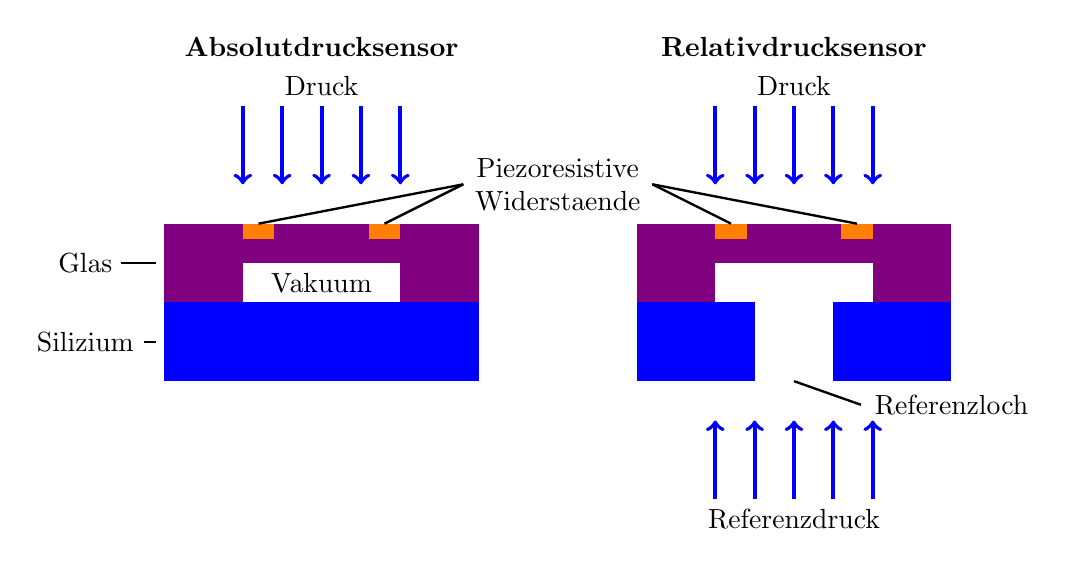
\begin{tikzpicture}
    % Absolutdrucksensor:
    
    % Zeichnen der Rechtecke
    \fill [blue] (0,0) rectangle ++(4,1);
    \fill [violet] (0,1) rectangle ++(4,1);
    \fill [white] (1,1) rectangle ++(2,0.5);
    \fill [orange] (1,2) rectangle ++(0.4,-0.2);
    \fill [orange] (3,2) rectangle ++(-0.4,-0.2);
    
    % Zeichnen der Beschriftungslinien
    \draw [black, line width=0.3mm] (-0.1,0.5) -- (-0.25,0.5);
    \draw [black, line width=0.3mm] (-0.1,1.5) -- (-0.55,1.5);
    
    % Zeichnen der Pfeile
    \foreach \i in {0,1,...,4}
    {
        \draw[blue, line width=0.5mm,->] ({1+\i*0.5},3.5) -- +(0,-1);
    }
    
    % Einfuegen der Beschriftungen
    \draw   (2,1.25) node {Vakuum}
    (2,3.75) node {Druck}
    (-1,0.5) node {Silizium}
    (-1,1.5) node {Glas}
    [font=\bfseries](2,4.25) node {Absolutdrucksensor};
    
    %%%%%%%%%%%%%%%%%%%%%%%%%%%%%%%%%%%%%%%%%%%%%%%%%%%%%%%%%%%%%%%%%%%%%%%%%%%%%%%%%%%%%
    % Relativdrucksensor:
    
    % Zeichnen der Rechtecke
    \fill [blue] (6,0) rectangle ++(4,1);
    \fill [violet] (6,1) rectangle ++(4,1);
    \fill [white] (7,1) rectangle ++(2,0.5);
    \fill [white] (7.5,0) rectangle ++(1,1);
    \fill [orange] (7,2) rectangle ++(0.4,-0.2);
    \fill [orange] (9,2) rectangle ++(-0.4,-0.2);
    
    % Zeichnen der Beschriftungslinien
    \draw [black, line width=0.3mm] (8,0) -- (8.85,-0.3);
    
    \draw [black, line width=0.3mm] (1.2,2) -- (3.8,2.5);
    \draw [black, line width=0.3mm] (2.8,2) -- (3.8,2.5);
    \draw [black, line width=0.3mm] (7.2,2) -- (6.2,2.5);
    \draw [black, line width=0.3mm] (8.8,2) -- (6.2,2.5);
    
    % Zeichnen der Pfeile
    \foreach \i in {0,1,...,4}
    {
        \draw[blue, line width=0.5mm,->] ({7+\i*0.5},3.5) -- +(0,-1);
        \draw[blue, line width=0.5mm,->] ({7+\i*0.5},-1.5) -- +(0,1);
    }
    
    % Einfuegen der Beschriftungen
    \draw   (8,3.75) node {Druck}
    (8,-1.75) node {Referenzdruck}
    (10,-0.3) node {Referenzloch}
    [align=center](5,2.5) node {Piezoresistive \\ Widerstaende}
    [font=\bfseries](8,4.25) node {Relativdrucksensor};
    
\end{tikzpicture}
    \caption{Aufbau des piezoresistiven Sensorchips}
    \label{fig:PIEZO}
\end{figure}

Bei piezoresistiven Druckmesszellen sind die Messwiderstände also im Gegensatz zum DMS in die Membran integriert. Bei dieser Technologie entfällt somit das Aufkleben, was eine wichtige Voraussetzung für Alterungs- und Temperaturbeständigkeit sowie Hysteresefreiheit (Hysterese = Nachwirkung des vorherigen Verformungszustands) ist. Das piezoresistive Messprinzip wird auch in dem DHT22-Sensor verwendet, was zu guten und genauen Messwerten führt \cite{Keller:2019}.

\section{Temperatur}

Die Temperaturmessung kann auf unterschiedliche Weise Erfolgen. Die verbreitetste ist das Flüssigkeitsthermometer, welches aus einem Vorratsgefäß und einem angeschlossenen Steigrohr, auch Kapillare genannt, besteht. Das Vorratsgefäß ist mit einer thermometrischen Flüssigkeit gefüllt, welche sich bei steigender Temperatur ausdehnt und das Steigrohr füllt.

Als alternative Möglichkeiten werden NTC- und PTC-Thermistoren verwendet. Auch genannt Heißleiter und Kaltleiter. Der NTC-Thermistor ist ein variabler elektrischer, wärmeempfindliche Widerstand, dessen Wert sich mit der Temperatur reproduzierbar ändert. Die Widerstände sind nicht linear und der Widerstand nimmt bei steigender Temperatur ab. Die Art und Weise, wie der Widerstand abnimmt, hängt mit einer Konstante zusammen, welche in der Elektroindustrie als Beta bekannt ist. Beta wird in Kelvin gemessen. Ein NTC ist also ein elektronisches Bauteil, welches den Widerstand temperaturabhängig verändert. Diese elektrischen Signale können dann Aufschluss über die Temperatur geben. Der PCT funktioniert vom Prinzip her gleich, jedoch steigt der Widerstand mit zunehmender Temperatur.

Leider wurde auf keiner Seite und in keinem Datenblatt veröffentlicht, um welches Prinzip es sich beim DHT22-Sensor handelt. Jedoch wurde nach der Recherche angenommen, dass ein NTC-Thermistor verbaut ist.  Dies wird dadurch begründet, dass keine Flüssigkeit im Sensor ist, und somit die erste Möglichkeit entfällt. Die Entscheidung gegen den PTC-Thermistor wurde getroffen, da PTC-Thermistoren Verhältnismäßig sehr teuer sind, und da der Sensor gerade einmal 7€ kostet, es sehr unwahrscheinlich ist, dass das Prinzip des PTC verwendet wurde \cite{Ametherm:2024}.

\section{Feuchtigkeit}

Es gibt vier Arten von Feuchtigkeitssensoren, die auf den Funktionsprinzipien und Sensormaterialien basieren: Kapazitiv, resistiv, Wärmeleitfähigkeit, psychometrisch. 

\subsection{Kapazitive Feuchtigkeitssensoren}

Kapazitive Feuchtigkeitssensoren gehören zu den am häufigsten verwendeten Arten. Dieses Prinzip ist auch im DHT22-Sensor verbaut. Die Sensoren funktionieren, indem sie Änderungen der Dielektrizitätskonstante eines Materials als Reaktion auf Änderung der Luftfeuchtigkeit messen. Die Dielektrizitätskonstante  misst die Fähigkeit eines Materials, elektrische Energie in einem elektrischen Feld zu speichern. 

Sie bestehen aus zwei Elektronen, wovon eins mit hygroskopischen Material beschichtet ist, dass Wasserdampf aus der Luft absorbiert. Wenn das hygroskopische Material Wasserdampf aufnimmt, führt dies zu einer Änderung der Dielektrizitätskonstante zwischen den beiden Elektroden, die vom Sensor gemessen wird. 

\subsection{Resistive Feuchtigkeitssensoren}

Resistive Feuchtigkeitssensoren, auch Hygrometer genannt, messen Änderungen im elektrischen Widerstand eines Materials als Reaktion auf der Änderung der Luftfeuchtigkeit. Die gebräuchlichste Art von Widerstandsfeuchtigkeitssensoren ist der polymerbasierte Sensor, welcher aus einem leitfähigen Polymerfilm besteht, der seinen Widerstand ändert, wenn er Wasserdampf ausgesetzt wird. 

Wenn der Polymerfilm Wasserdampf aus der Luft aufnimmt, schwillt er an und wird leitfähiger, wodurch der durch den Sensor fließende elektrische Strom zunimmt. Die Widerstandsänderung ist proportional zur Wasserdampfmenge in der Luft und kann zur Bestimmung der Luftfeuchtigkeit gemessen werden. Dieser Sensortyp ist auch in dem DHT22-Sensor verbaut und basiert auf diesem System. 

\subsection{Wärmeleitfähigkeits Feuchtigkeitssensor}

Wärmeleitfähigkeits-Feuchtigkeitssensoren messen die Wärmeleitfähigkeit eines Gasgemisches als Reaktion auf Änderungen der Luftfeuchtigkeit.Sie bestehen aus einem beheizten Sensorelement und einem Temperatursensor, der den Temperaturunterschied zwischen den Beiden misst. Wenn das Sensorelement Wasserdampf absorbiert, verringert es seine Wärmeleitfähigkeit, was zu einer Temperaturänderung führt, die der Temperatursensor messen kann. Diese Temperaturänderung ist proportional zur Menge an Wasserdampf in der Luft und kann zur Bestimmung der Luftfeuchtigkeit verwendet werden.

\subsection{Psychrometrische Feuchtigkeitssensoren}

Psychrometrische Feuchtigkeitssensoren, auch Taupunktspiegelsensoren genannt, messen die Temperatur, bei der Wasserdampf auf einer Oberfläche kondensiert.Sie bestehen aus einem gekühlten Spiegel, bis sich auf seiner Oberfläche Tau oder Reif bildet. Die Temperatur, bei der diese Kondensation auftritt, ist eine Funktion der relativen Luftfeuchtigkeit der Luft um den Spiegel \cite {Hengko:2024}.


\section{Sensor DHT22}

Der extern angeschlossene Sensor DHT22 ist für die Temperatur- und Luftfeuchtigkeitsmessung verantwortlich. Für den Betrieb wird die Bibliothek \FILE{DHT.h} benötigt, welche von Adafruit angeboten wird. Sie ermöglicht das starten und stoppen des Sensors, sowie das Auslesen der Temperatur und der Luftfeuchtigkeit. Die Bibliothek ist geeignet für die Sensoren vom Type DHT11 und DHT22.

\section{Schaltplan}

\begin{figure}[H]
    \begin{flushleft} 
        \centering
        \includegraphics[width=12cm]{Sensor/DHT22/Schaltplan.jpeg}
        \caption{Schaltplan des Raumklimamessgeraets}
        \label{fig:SP}
    \end{flushleft}
\end{figure}


\section{Testen des Sensors  DHT22}

Um die Funktion des LPS22HB-Sensors zu gewährleisten, wurde dieser an den Arduino angeschlossen und mit dem folgenden Programm getestet. Die gemessenen Werte werden seriell an den Computer weitergegeben und im Serial Monitor in der Arduino IDE angezeigt. Dieses Programm wurde zudem zur Kalibrierung verwendet.

\begin{lstlisting}[language=Arduino]
    // Einbinden von verwendeten Bibliotheken
    #include <DHT.h>
    
    // Einstellen des DHT22-Sensors
    #define DHTPIN D11   
    #define DHTTYPE DHT22    
    DHT dht(DHTPIN, DHTTYPE);
    
    void setup() {
        // Einschalten des Sensors
        pinMode(DHTPIN, INPUT);
        dht.begin();
    }
    
    void loop() {
        // Einstellen der Verzoegerung zwischen den Messvorgaengen
        delay(5000);
        
        // Auslesen der Messwerte durch den Sensor
        float humidity = dht.readHumidity(); 
        float temp = dht.readTemperature(); 
        
        // Messwerte seriell ausgeben
        Serial.print("Luftfeuchte: ");
        Serial.println(humidity);
        Serial.println();
        
        Serial.print("Temperatur: ");
        Serial.println(temp);
        Serial.println();
    }
\end{lstlisting}





\section{Kalibrierung}

\subsection{Opus20 THI} 

Das Opus 20 THI ist ein hochpräziser LAN-Datenlogger, der speziell zur Überwachung des Gebäudeklimas und zur Kontrolle klimasensitiver Produktionsprozesse entwickelt wurde. Es wird in EDV-Rechenzentren, Schaltschränken, Windturbinen, Lagerräumen und Museen eingesetzt. Das Gerät zeichnet sich durch seine Genauigkeit, Zuverlässigkeit und einfache Bedienung aus, siehe \ref{fig:Opus20THI}.

\begin{figure}[H]
    \centering
    \includegraphics[width=9cm]{Sensor/DHT22/Opus20THI.jpg}
    \caption{Opus 20 THI}
    \label{fig:Opus20THI}
\end{figure}

\subsection{Funktionen}

\subsubsection{Messparameter}

\begin{itemize}
    \item Temperatur
    \item Relative Feuchte
\end{itemize}

\subsubsection{Messtechnologie}

\begin{itemize}
    \item Temperatur: NTC 
    \item Relative Feuchte: Kapazitive Messung
\end{itemize}

\subsubsection{Produkt-Highlights}

\begin{itemize}
    \item LAN-Datenlogger mit eingebauten Sensoren
    \item Höchste Messgenauigkeit
    \item Firmware online aktualisierbar
    \item Verschiedene Stromversorgungsoptionen (USB, Batterien, PoE)
    \item Inklusive Auswertungssoftware SmartGraph3
\end{itemize}

\subsection{Schnittstellen}
\begin{itemize}
    \item USB (inkl. Kabel und SmartGraph3 Software)
    \item LAN
\end{itemize}

\subsection{Technische Daten}

\subsubsection{Allgemeine Daten}

\begin{itemize}
    \item Abmessungen: 166 x 78 x 32 mm
    \item Gewicht: ca. 250 g
    \item Gehäusematerial: Kunststoff
    \item Datenspeicher: 16 MB (3.200.000 Messwerte)
    \item Betriebsdauer mit Batterie: > 1 Jahr
    \item LC-Display: 90 x 64 mm
    \item Abtastintervalle: 10/30s, 1/10/12/15/30min, 1/3/6/12/24h
    \item Speicherintervalle: 1/10/12/15/30min, 1/3/6/12/24h
    \item Stromversorgung: 4 x LR6 AA Mignon, USB
    \item Betriebstemperaturbereich: -20 bis 50 °C
    \item Relative Feuchte: 0 bis 100 r.F., < 20g/m³ (nicht kondensierend)
    \item Maximale Höhe: 10.000m über Normal Null
\end{itemize}

\subsubsection{Temperaturmessung}

\begin{itemize}
    \item Messprinzip: NTC
    \item Messbereich: -20 bis 50 °C
    \item Einheit: °C
    \item Genauigkeit: ±0,3 °C (0 bis 40 °C), sonst ±0,5 °C
    \item Auflösung: 0,1 °C
\end{itemize}

\subsubsection{Feuchtemessung}

\begin{itemize}
    \item Messprinzip: Kapazitiv
    \item Messbereich: 0 bis 100 r.F.
    \item Einheit: r.F.
    \item Genauigkeit: ±2 r.F.
    \item Auflösung: 0,1 r.F.  \cite{Lufft:2018}
\end{itemize}

\subsection{Anwendung}

Das Opus 20 THI ist ideal für die Überwachung und Aufzeichnung von Klimadaten in kritischen Umgebungen, um optimale Bedingungen zu gewährleisten und Abweichungen frühzeitig zu erkennen. Die hohe Genauigkeit und die umfangreichen Schnittstellenoptionen machen es zu einem vielseitigen Werkzeug in der Klimakontrolle. Dies haben wir als Vorteil gesehen, um Referenzwerte für unser Gerät zu erlangen, um Anhand dessen unser Programm anpassen zu könne, um Korrekte Werte messen zu können. Unsere Kalibrierung erfolgte also auf Basis des hier genannten Opus 20 THI Datenloggers \cite{Daten:2024}.

\subsection{Kalibrierung}

Für die Kalibrierung des Raumklimamessgeräts wurden vorerst die Testprogramme für den DHT22- und den LPS22HB-Sensor verwendet. Es wurde in Abständen von ca. einer Stunde die Werte des OPUS20 THI und die des Raumklimamessgeräts abgelesen und in einer Tabelle gesammelt. Die Messergebnisse befinden sich in Documents/Messergebnisse\_OPUS.xlsx. Bei einer ausreichenden Anzahl an Werten wurde eine mittlere Abweichung der Messwerte berechnet und ausgegeben. Zudem wurden für die Messreihen Graphen erstellt. Es ist zu erkennen, dass in den vorliegenden Messbereichen eine relativ gleichbleibende Abweichung besteht, daher wurde die berechnete mittlere Abweichung einfach mit den gemessenen Werten der Sensoren addiert. Für die Messung der Temperatur wurde zusätzlich ein Messgerät von Philips verwendet, welches aber nicht weiter berücksichtigt wurde.

\begin{figure}[H]
    \centering
    \includegraphics[width=9cm]{Sensor/DHT22/AbweichungFeuchte}
    \caption{Graph für Abweichung der Luftfeuchtigkeit}
    \label{fig:ABWH}
\end{figure}

\begin{figure}[H]
    \centering
    \includegraphics[width=9cm]{Sensor/DHT22/AbweichungTemperatur}
    \caption{Graph für Abweichung der Temperatur}
    \label{fig:ABWT}
\end{figure}

\begin{figure}[H]
    \centering
    \includegraphics[width=9cm]{Sensor/DHT22/AbweichungDruck}
    \caption{Graph für Abweichung des Luftdrucks}
    \label{fig:ABWP}
\end{figure}
}

%\Ausblenden
{
\part{Anhang}

%  %%%%%%
%
% $Autor: Wings $
% $Datum: 2020-01-18 11:15:45Z $
% $Pfad: WuSt/Skript/Produktspezifikation/powerpoint/ImageProcessing.tex $
% $Version: 4620 $
%
%%%%%%


\chapter{Materialliste}



%\begin{table}
	\begin{longtable}{cp{6.1cm}p{2.5cm}c}
      \textbf{Anzahl} & \textbf{Bezeichnung} & \textbf{Link} & \textbf{Preis} \\ \hline      
      \multicolumn{4}{c}{\includegraphics[width=0.2\textwidth]{Nano33BLESense/ArduinoKit}} \\
      1      & ARD KIT TINYML Arduino - Lern-Kit Tiny Machine
             & \href{https://www.reichelt.de/arduino-lern-kit-tiny-machine-ard-kit-tinyml-p304338.html}{www.reichelt.de -  ARD Kit TinyML } 
             &  52{,}40 \euro{} \\ \hline 
      \multicolumn{4}{c}{\includegraphics[width=0.2\textwidth]{CAM/LensCalibrationTool/LensCalibrationTool}} \\
      1      & Arducam B0226 Lens Calibration Tool
& \href{https://www.welectron.com/Arducam-B0226-Lens-Calibration-Tool}{www.welectron.com -  Arducam B0226 Lens Calibration Tool } 
&  11{,}90 \euro{} \\ \hline
    \end{longtable}

Stand: 22.02.2023

%  \caption{Materialliste für die Applikation Bilderkennung}
%\end{table}




  %%%%%%
%
% $Autor: Wings $
% $Datum: 2020-01-18 11:15:45Z $
% $Pfad: WuSt/Skript/Produktspezifikation/powerpoint/ImageProcessing.tex $
% $Version: 4620 $
%
%%%%%%


\chapter{Datenblätter}

\section{Datenübersicht}

\newcounter{mycounter}

\setcounter{mycounter}{1}

\whiledo {\value{mycounter} < 4}
{
	\includegraphics[width=1\textwidth,page=\themycounter]{../../MLbib/Arduino/Nano33BLESense/ABX00031_ENG_TDS.pdf}
	\stepcounter{mycounter}
	\newpage
}



\setcounter{mycounter}{1}

\whiledo {\value{mycounter} < 2}
{
  \includegraphics[width=1\textwidth,page=\themycounter]{../../MLbib/Arduino/Nano33BLESense/Pinout-NANOsense_latest.pdf}
  \stepcounter{mycounter}
  \newpage
}

\setcounter{mycounter}{1}

\whiledo {\value{mycounter} < 2}
{
	\includegraphics[width=1\textwidth,page=\themycounter]{../../MLbib/Arduino/Nano33BLESense/NANO33BLE_V2.0_sch.pdf}
	\stepcounter{mycounter}
	\newpage
}
%
%\setcounter{mycounter}{1}
%
%\whiledo {\value{mycounter} < 12}
%{
%	\includegraphics[width=1\textwidth,page=\themycounter]{../../MLbib/Arduino/Portenta_H7_Web.pdf}
%	\stepcounter{mycounter}
%	\newpage
%}
%
%

  %%%%%%
%
% $Autor: Wings $
% $Datum: 2020-01-18 11:15:45Z $
% $Pfad: WuSt/Skript/Produktspezifikation/powerpoint/ImageProcessing.tex $
% $Version: 4620 $
%
%%%%%%


\chapter{\TRANS{Data Sheets}{Datenblätter} Arduino Vision Shield}


\newcounter{VScounter}
\setcounter{VScounter}{1}

\whiledo {\value{VScounter} < 9}
{
	\includegraphics[width=1\textwidth,page=\theVScounter]{../../MLbib/Arduino/ArduCAM/ArduCAM_Mini_2MP_Camera_Shield_DS.pdf}
	\stepcounter{VScounter}
	\newpage
}

\setcounter{VScounter}{1}

\whiledo {\value{VScounter} < 8}
{
	\includegraphics[width=1\textwidth,page=\theVScounter]{../../MLbib/Arduino/ArduCAM/ArduCAM_Mini_2MP_Camera_Shield_Hardware_Application_Note.pdf}
	\stepcounter{VScounter}
	\newpage
}

}

%\Ausblenden
{
  %%%%%%%%%%%%
%
% $Autor: Wings $
% $Datum: 2019-03-05 08:03:15Z $
% $Pfad: Batch.tex $
% $Version: 4250 $
% !TeX spellcheck = en_GB/de_DE
% !TeX encoding = utf8
% !TeX root = filename 
% !TeX TXS-program:bibliography = txs:///biber
%
%%%%%%%%%%%%


\section{Batch File}

\section{Batch File}

A batch file is a text file that contains a sequence of commands intended to be executed by the command-line interpreter. On Windows operating systems, these files typically have the extension \FILE{.bat} or \FILE{.cmd}. Batch files are used to automate repetitive tasks, perform complex sequences of commands, and streamline system administration processes. The results can be documented in a log file. 

\section{List Batch File}

A ``list batch file`` refers to a batch file designed to list specific items, such as files in a directory, the contents of a directory, or any other listable resources. In the context of Arduino CLI, a list batch file might include commands to list available Arduino boards, libraries, or sketches.

\begin{center}
    \begin{lstlisting}
@echo off
:: List available Arduino boards
arduino-cli board list
    \end{lstlisting}
\end{center}

\SHELL{@echo off} command is used at the beginning of the batch file to suppress the display of each command as it executes. By default, batch files echo each command to the console as they execute, but \SHELL{@echo off} prevents this behavior, making the output cleaner. 
\SHELL{:: List available Arduino boards} is a comment in the batch file. In batch scripting, comments start with :: or rem, and they are ignored by the command interpreter.
\SHELL{arduino-cli board list} command executes the arduino-cli command-line tool with the board list subcommand. This subcommand lists all available Arduino boards connected to the system

\subsection{Explanation of Batch commands}

This section describes how the batch script works.

{\small 
    \begin{lstlisting}
@echo off
echo log file Arduino setup, %time% clock, %date% > setup-log.txt
echo. >> setup-log.txt
echo. >> setup-log.txt
    \end{lstlisting}
}

The command \SHELL{\@echo off} prevents the script content from being output during execution. This enables more appealing front-end programming. The log file is created in the second line. When it is created, the first line of the log is given the heading \SHELL{Logfile Arduino setup} and the system time \SHELL{\%time\%} and date \SHELL{\%date\%} are read out. For later clarity of the log file, two empty lines \SHELL{echo. >> setup-log.txt}. If the greater than operator \SHELL{> setup-log.txt} is used once, a new file is created or an existing file with the same name is overwritten. If the greater than operator \SHELL{>> setup-log.txt} is used twice, the left-hand content is appended to an existing file in a new line. In this way, the log file is written line by line and not once completely at the end of the batch script.

\begin{center}
    \begin{lstlisting}
:: If necessary, the core is installed
echo core status: >> setup-log.txt
arduino-cli core install arduino:mbed_nano >> setup-log.txt
    \end{lstlisting}
\end{center}

Comments in the batch script are identified by two consecutive colons \SHELL{:: If necessary, the core is installed} and are intended to increase traceability within the script. The command \SHELL{echo core status: >> setup-log.txt} is used in the log file to indicate that the next line contains information about the core to be installed for the Arduino Nano 33 BLE Sense Lite. The Arduino CLI already has the intelligence to check whether the specified core is already installed. If this is the case, the corresponding documentation is included in the log file. The installation of the core is initialized with the line \SHELL{arduino-cli core install arduino:mbed\_nano >> setup-log.txt}. The core required for the Arduino Nano 33 BLE Sense Lite is specified with the name \SHELL{arduino:mbed\_nano}. The return value of the function for core installation is saved in the log file.

\begin{lstlisting}
echo A search is made for connected boards...
:: List the connected Arduinos
echo The following boards are connected to the PC: >> setup-log.txt
echo.
echo. >> setup-log.txt
arduino-cli board list >> setup-log.txt
arduino-cli board list
echo.
\end{lstlisting}

At the beginning of this script section, the user of the software is first informed about the search for the connected Arduino boards \SHELL{echo A search for connected boards is performed...}. The following command \SHELL{echo The following boards are connected to the PC: >> setup-log.txt} informs the user about the content of the next line in the log file. Information about which Arduinos are connected to the PC can be obtained with the command \SHELL{arduino-cli board list}, which is executed twice here. In the first execution, the return of the Arduino-CLI is saved in the log file \SHELL{>> setup-log.txt}, the second execution is used for display in the currently executed script. The user needs the information about the connected Arduinos for an input in the next step.

\begin{lstlisting}
:: Query the port name for later upload 
:: of the sensor test file
set /p port="Please enter the port name of the Sense-Lite and confirm: "
echo The port %port% was selected. >> setup-log.txt
\end{lstlisting}

In the line \SHELL{set /p port="Please enter the port name of the Sense-Lite and confirm:"} a user query is displayed. The command \SHELL{set} allows the variable \SHELL{port} to be set to a specific value. With the addition \SHELL{/p}, this specific value is set to the following user input. Execution of the script is stopped until the user input is successful. The user input contains the port of the connected Arduino Nano 33 BLE Sense Lite. For later traceability, the selected port is entered in the log file with the line \SHELL{echo The port \%port\% was selected. >> setup-log.txt} is documented. 

\begin{lstlisting}
:: Create the folder for the compiled sensor test
set folder=SensorTestCompiledData
mkdir %folder%
\end{lstlisting}
The variable \SHELL{ordner} is assigned the value \SHELL{SensorentestCompiledData}. In the next line \SHELL{mkdir \%folder\%} the folder with the name \PYTHON{SensorentestCompiledData} is created for saving the compiled sketch later.

\begin{lstlisting}
:: If necessary, the required libraries for 
:: the sensor test are installed
:: Bib for IMU
echo Bib for IMU >> setup-log.txt
arduino-cli lib install Arduino_LSM9DS1 >> setup-log.txt
echo. >> setup-log.txt
    
:: Bib for color sensor
echo Bib for color sensor >> setup-log.txt
arduino-cli lib install Arduino_APDS9960 >> setup-log.txt
echo. >> setup-log.txt
    
:: Bib for pressure and temperature sensor
echo Bib for pressure and temperature sensor >> setup-log.txt
arduino-cli lib install Arduino_LPS22HB >> setup-log.txt
echo. >> setup-log.txt
\end{lstlisting}

The log file documents which library is involved in the following line \SHELL{SensorentestCompiledData}. Then use the command \SHELL{arduino-cli lib install Arduino\_LSM9DS1 >> setup-log.txt} to install the library and save the return value of the installation in the log file. A library that has already been installed is recognized by the Arduino CLI and a corresponding return value is written to the log file. The procedure is identical for all three libraries to be installed.

\begin{lstlisting}
:: Compiling the sensor test sketch
echo Compiling the sensor test sketch: >> setup-log.txt
echo. >> setup-log.txt
arduino-cli compile -b arduino:mbed_nano:nano33ble 
%cd%\SensortestLite 
--build-path %cd%\%folder% >> setup-log.txt
\end{lstlisting}

Once the necessary libraries have been installed, the previously created sketch for testing the sensors can be compiled. The sketch for the Arduino Nano 33 BLE Sense Lite is compiled with the command \SHELL{arduino-cli compile -b arduino:mbed\_nano:nano33ble \%cd\%/SensortestLite}. The last part of the command specifies the memory path of the sketch to be compiled. Furthermore, the target folder for the compiled sketch can be defined with the addition \SHELL{--build-path \%cd\%/\%folder\% >> setup-log.txt}. The return value of compiling with the Arduino CLI is saved in the log file.

\begin{lstlisting}
:: Upload the compiled sketch to the Arduino
echo Upload the compiled sketch to the Arduino >> setup-log.txt
arduino-cli upload -p %port% --input-dir %cd%\%folder% 
>> setup-log.txt
\end{lstlisting}

The compiled sketch is stored in the line \SHELL{arduino-cli upload -p \%port\% --input-dir}  \SHELL{\%cd\%/\%folder\% >> setup-log.txt} to the Arduino Nano 33 BLE Sense Lite connected via \SHELL{port}. The storage path of the compiled data is specified with the addition \SHELL{--input-dir \%cd\%/\%folder\%}.

\begin{lstlisting}
:: Opening the serial monitor
start monitor_log
:: Automatic closing of the serial monitor after 4 seconds 
:: (n-1 seconds, with n=5)
ping 127.0.0.1 -n 5 > nul
taskkill /im serial-monitor.exe /F
\end{lstlisting}

The command \SHELL{start monitor\_log} calls another batch script to read out the serial monitor. The line \SHELL{ping 127.0.0.1 -n 5 > nul} stops the execution of the software for four seconds. Five requests are sent to the local computer and one second is waited between each request. With \SHELL{> nul}, the output of the responses is directed to the void and not displayed. Once the four-second period has elapsed, the serial monitor for reading the sensor data is automatically closed with the command \SHELL{taskkill /im serial-monitor.exe /F}. The window to be closed can be named \SHELL{serial-monitor.exe} using the suffix \SHELL{/im}. The forced closing of the serial monitor takes place with the appendix \SHELL{/F}. After the serial monitor has been read out and closed, the software can be closed. The results of the sensor test can then be found in the log file.

The serial monitor is opened in the script \FILE{monitor\_log.bat}.

\begin{lstlisting}
echo Sensor data: >> setup-log.txt
echo. >> setup-log.txt
    
echo The serial monitor is opened, the sensor data is 
read out and saved in the log file...
    
arduino-cli monitor -p %port% >> setup-log.txt
\end{lstlisting}	

The serial monitor can be activated using the Arduino CLI command \SHELL{arduino-cli monitor} \SHELL{-p \%port\% >> setup-log.txt} to open it. The connection for the specified port is established with \SHELL{-p \%port\%}. With the addition \SHELL{>> setup-log.txt} the received data is written to the log file.

}

%\addcontentsline{toc}{chapter}{Literaturverzeichnis}

\printbibliography[
heading=bibintoc,
title={Literaturverzeichnis}
]


\newpage

\addcontentsline{toc}{chapter}{Stichwortverzeichnis}
\printindex

%\part{Anhang}


%%\input{todo}
%


\end{document}
